\documentclass[
  11pt,
	colorful,
	raggedright,
  % boxey,
  % oneside % screws things up because of spacing
  % raggedbottom,
]{tufte-style-thesis-flip}

\usepackage[
  autocite  = superscript,
  backend   = biber,
  citestyle   = numeric-comp,
  style     = numeric,
  sorting   = none,
  bibencoding = utf8,
]{biblatex}

%!TEX root = paper.tex
%% FLIP’S PREAMBLE; 
%% Use FlipAdditionalHeader for project-specific packages & macros

% \pdfoutput=1 % for JHEP

%%%%%%%%%%%%%%%%%%%%%%%%%%
%%%  COMMON PACKAGES  %%%%
%%%%%%%%%%%%%%%%%%%%%%%%%%

\usepackage{amsmath}
\usepackage{amssymb}
\usepackage{amsfonts}
\usepackage{graphicx}
% \usepackage[utf8]{inputenc}     % inspire bibs
\usepackage{aas_macros}				  % ads bibs
\usepackage{bm}      
\usepackage{fix-cm}            % \boldsymbol
\usepackage{amsthm}
\usepackage{microtype}

%%%%%%%%%%%%%%%%%%%%%%%%%%%
%%%  UNUSUAL PACKAGES  %%%%
%%%%%%%%%%%%%%%%%%%%%%%%%%%

%% MATH AND PHYSICS SYMBOLS
%% ------------------------
\usepackage{slashed}				% \slashed{k}
\usepackage{mathrsfs}				% Weinberg-esque letters
\usepackage{bbm}					  % \mathbbm{1} conflict: XeLaTeX 
\usepackage{cancel}					
\usepackage[normalem]{ulem} % for \sout
\usepackage{youngtab}	    	% Young Tableaux
% \usepackage{isomath}            % for styling vectors

%% CONTENT FORMAT AND DESIGN
%% -------------------------
% \usepackage[dvipsnames]{xcolor} % OPTION CLASH
% \usepackage[hang,flushmargin]{footmisc} % OPTION CLASH

% \usepackage{fancyhdr}		% preprint number
\usepackage{lipsum}			% block of text 
\usepackage{framed}			% boxed remarks / Next time: use mdframed
                        % https://github.com/marcodaniel/mdframed/blob/master/mdframed.pdf
% \usepackage{subcaption}	% subfigures
% \usepackage{cite}			  % group cites
\usepackage{xspace}			% macro spacing


%% TABLES IN LaTeX
%% ---------------
\usepackage{booktabs}		% professional tables
\usepackage{nicefrac}		% fractions in tables,
\usepackage{multirow}		% multirow elements in a table
\usepackage{arydshln}		% dashed lines in arrays

%% ARRAY STRETCH: vertical spacing between rows
% \renewcommand{\arraystretch}{1.5} %% put this in main text

%% Other Packages and Notes
%% ------------------------
% \usepackage[font=small]{caption} 	% caption font is small
% \usepackage{float}         			  % for strict placement e.g. [H]


%%%%%%%%%%%%%%%%%%%%%%%%%%%%%%
%%%  DOCUMENT PROPERTIES  %%%%
%%%%%%%%%%%%%%%%%%%%%%%%%%%%%%

% \usepackage[margin=2.5cm]{geometry} % margins
\graphicspath{{figures/}}			      % figure folder
% \numberwithin{equation}{section}    % set equation numbering
% \usepackage{marginnote}             % for \marginnote{comment}
% \usepackage{mparhack}               % fix for \marginnote
% \usepackage{marginfix}              % fix for \marginnote
% \usepackage{adjustbox}              % to rescale elements



%% References in two columns, smaller
%% http://tex.stackexchange.com/questions/20758/
% \usepackage{multicol}
% \usepackage{etoolbox}
% \usepackage{relsize}
% \patchcmd{\thebibliography}
%   {\list}
%   {\begin{multicols}{2}\smaller\list}
%   {}
%   {}
% \appto{\endthebibliography}{\end{multicols}}


% % Change list spacing (instead of package paralist)
% % from: http://en.wikibooks.org/wiki/LaTeX/List_Structures#Line_spacing
% % alternative: enumitem package
% \let\oldenumerate\enumerate
% \renewcommand{\enumerate}{
%   \oldenumerate
%   \setlength{\itemsep}{4pt}
%   \setlength{\parskip}{0pt}
%   \setlength{\parsep}{0pt}
% }

% \let\olditemize\itemize
% \renewcommand{\itemize}{
%   \olditemize
%   \setlength{\itemsep}{4pt}
%   \setlength{\parskip}{0pt}
%   \setlength{\parsep}{0pt}
% }

%% FOR DRAFT EDITING AND DISCUSSION
\usepackage{lineno}
% \linenumbers          %% put this in main text


%%%%%%%%%%%%%%%%%%%%%%%%%%%
%%%  (RE)NEW COMMANDS  %%%%
%%%%%%%%%%%%%%%%%%%%%%%%%%%

%% FOR `NOT SHOUTING' CAPS (e.g. acronyms)
%% ---------------------------------------
\usepackage{scalefnt} 
\newcommand\acro[1]{{\footnotesize #1}}           % acronyms in footnote size


%% COMMON PHYSICS MACROS
%% ---------------------
% \renewcommand{\tilde}{\widetilde}   % tilde over characters
%% doesn't seem to work with the default tufte-thesis font
\renewcommand{\text}{\textnormal}	% text in equations 
% \renewcommand{\vec}[1]{\mathbf{#1}} % vectors are italic boldface
\renewcommand{\vec}[1]{\boldsymbol{#1}} % vectors are italic boldface
% \renewcommand{\vec}[1]{\mathbfit{#1}} % using isomath; buggy

%% For ISO tensor guidelines
\DeclareMathAlphabet{\mathsfit}{T1}{\sfdefault}{\mddefault}{\sldefault}
\SetMathAlphabet{\mathsfit}{bold}{T1}{\sfdefault}{\bfdefault}{\sldefault}
\newcommand{\tensor}[1]{\mathsfit{#1}} % vectors are boldface

% \newcommand{\dbar}{d\mkern-6mu\mathchar'26}    % for d/2pi
\newcommand{\dbar}{d\mkern-6mu\mathchar'26\hspace{-.1em}}    % fixed spacing
\renewcommand{\ket}[1]{\left|#1\right\rangle}    % <#1|
\renewcommand{\bra}[1]{\left\langle#1\,\right|}    % |#1>

%% COMMANDS FOR TEMPORARY COMMENTS
%% -------------------------------
\newcommand{\comment}[2]{\textcolor{red}{[\textbf{#1} #2]}}
\newcommand{\flip}[1]{{
	\color{green!50!black}
  \footnotesize
  [\textbf{\textsf{Flip}}: \textsf{#1}]
	}}


%% COMMANDS FOR TOP-MATTER
%% -----------------------
\newcommand{\email}[1]{\href{mailto:#1}{#1}}
\newenvironment{institutions}[1][2em]{\begin{list}{}{\setlength\leftmargin{#1}\setlength\rightmargin{#1}}\item[]}{\end{list}}


%% COMMANDS FOR LATEXDIFF
%% ----------------------
%% see http://bit.ly/1M74uwc
\providecommand{\DIFadd}[1]{{\protect\color{blue}#1}} %DIF PREAMBLE
\providecommand{\DIFdel}[1]{{\protect\color{red}\protect\scriptsize{#1}}}

%% REMARK: use latexdiff option --allow-spaces
%% for \frac, ref: http://bit.ly/1iFlujR
%% Errors with environments? https://tex.stackexchange.com/q/73224

%% USAGE: latexdiff draft.tex revision.tex > diff.tex

% %%%%%%%%%%%%%%%%%%%%%
% %%%  TITLE DATA  %%%%
% %%%%%%%%%%%%%%%%%%%%%

% %% PREPRINT NUMBER USING fancyhdr
% %% Don't forget to set \thispagestyle{firststyle}
% %% ----------------------------------------------
% \renewcommand{\headrulewidth}{0pt} 	% no separator
% \setlength{\headheight}{15pt} 		% min to avoid fancyhdr warning
% \fancypagestyle{firststyle}{
% 	\rhead{\footnotesize%
% 	\texttt{\FlipTR}%
% 	}}

% %% TOC overwrites fancyhdr, here's a fix
% %% http://tex.stackexchange.com/questions/167828/
% \usepackage{etoc}
% \renewcommand{\etocaftertitlehook}{\pagestyle{plain}}
% \renewcommand{\etocaftertochook}{\thispagestyle{firststyle}}
\newtheorem{exercise}{Exercise}[section]
\newtheorem{example}{Example}[section]

% Flip's stuff
% This doesn't work with the default Linux Libertine font :()
% \renewcommand{\dbar}{d\mkern-6mu\mathchar'26\hspace{-.1em}}    % for d/2pi
% Hack: https://tex.stackexchange.com/a/203511
\renewcommand{\dbar}{d\hspace*{-0.08em}\bar{}\hspace*{0.1em}}  
% See discussion in stackexchange

% For matrices
\newcommand{\aij}[2]{^{#1}_{\phantom{#1}#2}}
\newcommand{\mat}[3]{#1\aij{#2}{#3}}

% Bold italic math: https://tex.stackexchange.com/a/82747/8094
\DeclareMathAlphabet{\mathbfsf}{\encodingdefault}{\sfdefault}{bx}{n}
\newcommand{\tens}[1]{\mathbfsf{#1}}


%	package inclusions for this specific documentation file. the .cls does not neet them.
\usepackage{lipsum}		% the chad package
\usepackage{textgreek}	% for greek
\usepackage{imakeidx}	% for index
\usepackage{multicol}
% \usepackage{bibentry}
\makeindex[columns=3]

\addbibresource{refs.bib} % for biblatex
% NOTE: sometimes biber has problems
% https://tex.stackexchange.com/a/135496/8094 clearing cache helps

% INFO : used in the titlepage, copyright and stuff.
\author{Flip Tanedo}
\title{Physics 231: Methods of Theoretical Physics}
\subtitle{A mathematical methods course for first-year graduate students in physics \& astronomy}
\university{University of California, Riverside}
\lab{Physics 231, Fall 2022}
\logo{figures/FlipAmbigram.png}
\type{Lecture Notes}

\begin{document}

\maketitle

\frontmatter

\chapter{Abstract}
Physics 231 is a crash course on mathematical methods necessary to succeed in the first-year physics graduate curriculum at \acro{UC~R}iverside. 
%
The focus is how to solve differential equations using Green's functions. This version is revised for Fall 2022. Last Compiled: \today




\tableofcontents
% \listoffigures
% \listoftables
% \listoflistings


\mainmatter

\chapter{Mathematical Methods}

This is a \emph{crash course} on the mathematical toolkit necessary for graduate courses in electrodynamics, quantum mechanics, and statistical mechanics. The emphasis is physical intuition rather than mathematical rigor. Let us be clear: as a student you are \emph{expected} to be as mathematically rigorous as your discipline requires. Fortunately, there are plenty of excellent textbooks pitched at various levels of rigor and you can find the one most appropriate for you. This course is meant to complement those references, not to replace them.\footnote{In other words, this is \emph{your} \acro{Ph.D}, craft it appropriately.}

Unfortunately for you, it is unlikely that the choice of topics in this course will be either necessary or sufficient for your training. If anyone asks, you should say that the theme of this course is to solve the types of linear differential equations that will show up in your physics coursework (\emph{ugh! Boring!}). The actual choice of topics is meant to highlight big, unifying themes in mathematical physics sprinkled with topics of current research significance.

\section{Green's functions and this course}

Our goal is to solve linear differential equations:
\begin{align}
  \mathcal O f(x) = s(x) \ .
  \label{eq:greens:function:equation}
\end{align}
In this equation, $\mathcal O$ is a \emph{differential operator}\index{differential operator} that encodes some kind of physical dynamics\footnote{A \textbf{differential operator} is just something built out of derivatives that can act on a function. The differential operator may contain coefficients that depend on the variable that we are differentiating with respect to; for example, $\mathcal O = (d/dx)^2 + 3x\,(d/dx)$.}, $s(x)$ is the \emph{source} of those dynamics, and $f(x)$ is the system's physical \emph{response} that we would like to determine. The solution to this equation is:
\begin{align}
  f(x) &= \mathcal O^{-1} s(x) \ .
\end{align}
This statement is trivial and deeply unsatisfying. We will think carefully about what $\mathcal O^{-1}$ actually means and how to calculate it. $\mathcal O^{-1}$ is the \textbf{Green's function}\index{Green's function} for the differential operator $\mathcal O$. %In this course, we use the quest to understand Green's functions to guide our study of mathematical physics.

\begin{exercise}
Consider the differential operator $\mathcal O = (d/dx)^2 + 3x\,(d/dx)$. A colleague tells you that $(d/dx)^2$ is squared, therefore it is not a linear operator. Explain why the colleague is mistaken. 
\end{exercise}

To make sense of $\mathcal O^{-1}$, we appeal to linear algebra. A linear transformation---that is, a \textbf{matrix}---$A$ acts on a vector $\vec{v}$ to give equations like
\begin{align}
  A \vec{v} = \vec{w} \ ,
\end{align}
whose solution is
\begin{align}
  \vec{v} = A^{-1} \vec{w} \ .
\end{align}
In this course, we think of linear differential operators $\mathcal O$ as infinite-dimensional matrices. $\mathcal O^{-1}$ is the inverse of this matrix. At this point, you should feel a bit nervous because you remember that inverse of a $3\times 3$ matrix is tricky... say nothing of the \emph{infinite} dimensional limit. We remember, however, that calculus is infinite-dimensional linear algebra. Complex analysis extends the real line to the complex plane. In so doing, the \emph{analytic structure} of our theories offer both a method to calculate challenging integrals and their own physical significance. 

Our simple example through this journey is the humble harmonic oscillator. In subsequent chapters we extend this to higher-dimensions and, indeed, to \emph{infinite} dimensions. Along the way we reflect on the nature of all of these infinities we bandy about. We close by connecting our study of Green's functions to statistics, non-perturbative methods, and the burgeoning connections of physics to machine learning.

\section{This is not what I expected}


This is a course in mathematical methods for \emph{physicists}.
%
We do not solve \emph{every} class of differential equation that is likely to pop up in your research careers---that would be a course on mathematical methods for \emph{engineers}. (I recommend Carl Bender's 2011 lectures at \acro{PSI} for an insightful course along those lines.\sidecite{pirsa_11110040}) Instead, we methodically dissect a physically motivated example---the harmonic oscillator---to emphasize how we think about mathematical problems. 

We weave together ideas that are not often connected explicitly in undergraduate physics courses: linear algebra, differential equations, complex analysis, statistics. I expect that you have had some formal training in these topics so that we may focus on the interconnections between these ideas and how those interconnections come up over and over again in our study of nature.

Do not be surprised if we only mention Bessel functions in passing. Do not think less of our efforts if we do not calculate Wronksians or go beyond a single Riemann sheet. As graduate students, it is \emph{your} responsibility to be able to grab your favorite reference to apply mathematics as needed to \emph{your} research. \emph{This} course is about the larger narrative that is not often shared explicitly in those books. It is about that which makes physicists employable in Silicon Valley while simultaneously terrible at splitting the bill at a restaurant. 

\begin{example}
Our cavalier attitude towards mathematical rigor should not make you think that mathematical rigor is not necessary. For a nice, visual example, see ``How to lie using visual proofs'' by 3Blue1Brown.\cite{3Blue1Brown_2022}
% https://youtu.be/VYQVlVoWoPY
\end{example}
 


\section{The non-mathematical idea  of mathematical niceness}
\label{sec:niceness}

I find it useful to appeal to the notion of a \textbf{nice}\index{nice} mathematical situation. This is not a formal idea. In fact, it is one many things that mathematicians find ridiculous about me. But as a physicist, the concept of mathematical \emph{niceness} is remarkably helpful.

The physical systems that we spend the most time thinking about are all \emph{nice}. 
%
While our mathematical cousins spend years proving every exceptional case to a theorem, we tend to be happy to push onward as long as mathematical results are true for the \emph{nice} cases. 
%
In fact, nature often admits an \emph{approximately} nice mathematical description.\footnote{This is not because nature is kind, but rather because we are only clever enough to build simple theories. What is important to appreciate as a student is \emph{why} simple theories can so nearly approximate nature.}

%
Nice mathematical models make tidy predictions. Then we can Taylor expand about these nice predictions to make better predictions.
%
We sometimes chant \emph{perturbation theory}\index{perturbation theory} out loud several times in case someone watching us does not think we are being rigorous enough.\footnote{Sometimes our Taylor expansions have zero radius of convergence. ``\emph{E pur si muove},'' as Galileo would say.}
% We make Taylor expansions without anguishing about the radius of convergence\footnote{\url{https://johncarlosbaez.wordpress.com/2016/09/21/struggles-with-the-continuum-part-6/}} and validate it post-facto because it \emph{works}.


This is not to say that nature cares at all about our physical models. 
%
Every once in a while, we \emph{do} have to worry about the exceptional cases because our models fail to accommodate what is \emph{actually} happening in nature.\footnote{Full disclosure? Your \acro{Ph.D} will likely depend on finding a clever solution to one of these cases.} Those scenarios are the most exciting of all: that is when our mathematical formalism grabs us by the collar and says, \emph{listen to me---something important is happening!} This often happens when a calculation tells us that a physical result is infinite. 

\begin{exercise}\label{ex:hydrogen:problem}
Consider the potential that an electron feels in the hydrogen atom:
\begin{align}
  V(r) &= -\frac{\alpha}{r} \ .
\end{align}
As the electron--proton separation goes to zero, $r\to 0$, the potential goes to infinity. Classical electrodynamics is telling us that something curious is happening. What actually happens? (And why didn't you ask this question when you were in high school?)
\end{exercise}

We focus on \emph{nice} functions and \emph{nice} operators and \emph{nice} boundary conditions, and so forth. We often only need the \emph{nice} math to make progress on our \emph{nice} physical models. It is worth spending our time learning to work with these \emph{nice} limits. Leave the degenerate cases to the mathematicians for now. Eventually, you will find yourself in a situation where physics demands \emph{not nice} mathematics. In that case---and only when the physics demands it---you will be ready to poke and prod at the mathematical curiosity until the underlying \emph{physics} reason for the not-niceness is apparent. All this is to say: if you object to this course because we do not start with proofs about open sets or convergence, then you are missing the point of an education in physics.

\section{The unbearable arrogance of physicists}
\label{sec:obvious}

Sometimes we, as physicists, have a reputation for arrogance. The most generous interpretation is that we must have some Promethean \emph{chutzpah} to seek to comprehend/invent/discover an underlying mathematical organizing principle for the universe. On the other side of this is the damaging ways in which scientists can mistreat each other in academia. Somewhere in between are footnotes poking fun at mathematicians, or being a bit of a bore at parties. But these are lecture notes about mathematical physics; it is up to you to figure out how to be the best version of you-as-physicist-and-human-being that you can realize.\footnote{There are plenty of excellent pieces to reflect on this. For example, \emph{The Disordered Cosmos}, \emph{The Only Woman in the Room}, and \emph{Beamtimes and Lifetimes}.}

What is within the scope of a set of lecture notes on mathematical physics is the apparent arrogance about the way we speak and write about technical ideas. In particular, the arrogance of phrases like \emph{it is obvious that$\ldots$}. In colloquial conversation, these phrases are smug or aggressive: \emph{look how smart I am that I comprehend this so easily!}\footnote{In my youth I would often curse at my textbooks: \emph{If it's so obvious, then why don't you explain it, you lazy asshole!}} In a graduate course, however, this sentiment means something very specific with pedagogical value. When these notes say that something is \emph{obvious}\index{obvious} or \emph{clear}, what we really mean is the following:
\begin{quote}
If you think about this idea with a certain perspective, then the idea is self-evident in a way that is illuminating. However, there are many other perspectives in which the idea is unclear. If you find the idea unclear, do \emph{not} assume that the idea itself is esoteric or that you are somehow deficient. Instead, take a step back to see if the idea is a natural consequence of a different approach. 
\end{quote}
Any time that these notes refer to being \emph{obvious}, it is a checkpoint. When something is not obvious, it is an invitation to reflect and perhaps backtrack a bit. In fact, when something is not obvious, it is an \emph{opportunity} to understand the idea more deeply---for now you have seen how the idea can become apparently complex, but you are being assured that in this complexity there is a underlying simple organizing principle. What can be more tantalizing than that?

There is a complementary idea that students have a secret superpower that they can exercise in the classroom. It is terrifying to ask questions in public---after all, what if your peers decide that you must be \emph{stupid}? There is didactic armor against this. Whenever you are confused, and at the first appropriate moment after you are confused, raise your hand and phrase your question as follows:
\begin{quote}
\emph{Is it obvious that} $\ldots$ ?
\end{quote}
Linguistically, this is a trick of the passive voice: it removes \emph{you} from the query. It does not insist that you are incapable of comprehending something, it simply asks if there is some intuitive understanding that you want to make sure you do not miss. After all, developing your physics intuition is one of the goals of your first-year graduate courses. Any self-respecting instructor will respond sympathetically, either:
\begin{itemize}
  \item \emph{no}, it is not obvious. Perhaps then you work through the idea carefully. Or,
  \item \emph{yes}, it is obvious---but only when we remember some previous key step, which your instructor should then highlight.
\end{itemize}
Either way, the result is wisdom rather than risking how you look in front of your peers. 

By the way, \emph{how you look in front of your peers} is not a good reason to do anything. It is almost as bad as not asking questions because you do not want to look stupid in front of your advisor. Here is some free advice: your adviser knows \emph{exactly} how stupid you are. Most likely your advisor does not think you are stupid, but if you are convinced that you are stupid, then rest assured that your advisor knows this and has still chosen to invest their time into you. Make the most of this time: ask questions.


\section{Footnotes}

I tend to be verbose with foot/margin-notes.\footnote{\emph{Pale Fire}, V.~Nabokov.} There are a few types of marginalia:
\begin{itemize}
  \item References, so you do not have to flip back to a bibliography at the end of the document.
  \item Enigmatic hints of how ideas interconnect. This document's main narrative focuses on first-year graduate physics, but because so many of the ideas here reappear in more advanced topics, I cannot help but mention a few of them in passing. These notes seem more mysterious than pedagogical to those who have not studied those topics; please take this as an invitation to dig deeper into the topic if it excites you.
  \item Miscellaneous examples or observations that are not germane to the specific topic in the main text, but are worth highlighting for the eager student.
  \item Miscellaneous personal reflections with no pedagogical value other than to remind the reader that the human being writing these notes was once a beginner student as well.
\end{itemize}

\section{One last piece of advice}

It took me way too long to appreciate the crucial significance of homework and exercises in learning physics. Your job in your \acro{Ph.D} is to answer questions where no previous answer had ever existed in the history of humanity. You will be guided by your advisor and your mentors, but you will be the discover-er of truth. This is a tall order, something like completing a marathon or climbing Everest. And like those physical feats, the only way to succeed in your intellectual pursuit is to \emph{train}. And the best training we have in physics are practice problems. These are problems that are crafted to hone your skills. They are examples that are assured to be \emph{solvable}\footnote{The fact that they are solvable does not mean that you are entitled to a solution set other than the solution that you earn by deriving it yourself.} and with a framework (like a course with peers) to guide you through the challenges. Do not squander the opportunity to \emph{train}. My undergraduate advisor used to say, \emph{you should do every problem in the book---but especially the ones that you cannot do.}



\chapter{Physics versus Mathematics} 

Let us make one point clear:
\begin{align}
  \text{Physics} \neq \text{Mathematics} \ .
\end{align}
This is a truth in many different respects\footnote{The astronomer Fritz Zwicky would perhaps call this a \emph{spherical truth}; no matter how you look at it, the statement is still true.}:
\begin{itemize}
  \item Physicists are rooted in experimental results. {Even theorists? \emph{Especially} theorists.}
  
  \item Physicists Taylor expand to their hearts’ content. Even when it is sometimes not mathematically valid.~\sidecite{Baez_Azimuth_2016}

  \item Physicists pick a basis, use coordinates, and decorate every tensor with indices. {Equations in physics appear intimidating because of the indices decorating our variables. Ironically, physicists are often intimidated by mathematics because of the conspicuous absence of any indices.}.

  \item Physicists seek truths about \emph{this} universe.

  \item Physicists have a fast and loose relationship to the concept of infinity and the related concept of the infinitesimal---on this, I recommend Jim Holt's essay ``The Dangerous Idea of the Infinitesimal.''~\sidecite{holt2018einstein}
  At the same time, many of our tools seem to \emph{beg} questions about the infinite.
\end{itemize}
My friends, we are not doing mathematics. 

\section{The most important binary relation}

When we write equations, the symbol that separates the left-hand side from the right-hand side is a binary relation. We use binary relations like $=$ or $\neq$. Sometimes to make a point we write $\cong$ or $\equiv$ or $\dot =$ to mean something like `definition’ or `tautologically equivalent to’ or some other variant of \emph{even more equal than equal}. 

 \begin{figure}[h]
      \sidecaption{Mathematical symbol fight from \acro{XKCD}.~\cite{xkcd_2343} \acro{CC BY-NC 2.5} \label{fig:xkcd:symbol}} % put this on top
      % \label HAS to be inside the \sidecaption
      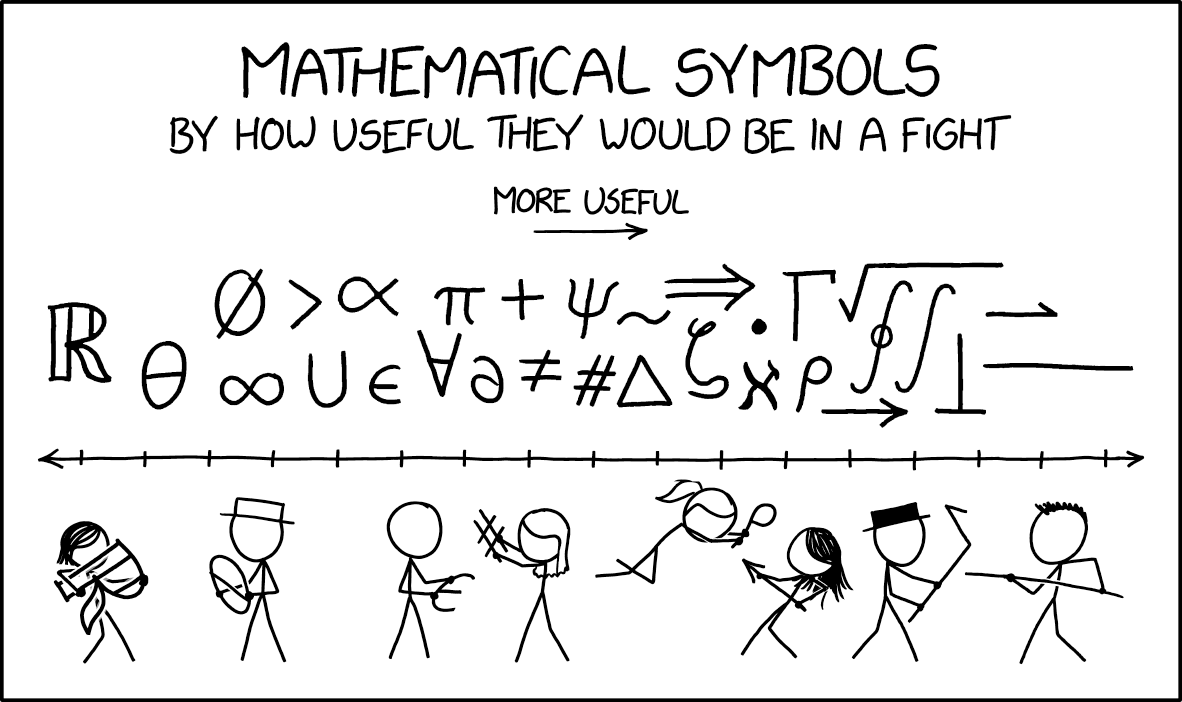
\includegraphics[width=\textwidth]{mathematical_symbol_fight_2x.png} % or tikz or anything
  \end{figure}
% xkcd_2343

As physicists the most important binary relation is none of those things\footnote{I thank Yuval Grossman teaching me this.}. What we usually care about is  $\sim$.\footnote{I use this the same way as $\propto$, which is completely different from `approximately,’ $\approx$.} The symbol $\sim$ tells us how how something \emph{scales}. If I double a quantity on the right-hand side, how does the quantity on the left-hand side scale? Does it depend linearly? Quadratically? Non-linearly? The answer encodes something important about the underlying physics of the system. The symbol $\sim$ the reason why \emph{imagine the cow is a sphere} is a popular punchline in a joke about physicists. 


Implicit in this discussion is the pragmatic policy that we will not care about stray factors of 2 in this class. As my adviser used to say, if you are worried about a factor of 2, then you have addition homework to figure out that factor of 2.\footnote{That being said, you are reading these notes and find an error, do let me know about it.} 

\section{Units}

There is another way in which physics is different from mathematics. It is far more prosaic. \emph{Quantities in physics have units}. We do deal in simply numbers, we deal with kilograms, electron volts, meters. It turns out that dimensional analysis is a big part of what we do as physicists. 

\begin{exercise}
Explain, in words, why the quantity $\sin(3~\text{cm})$ is absolute nonsense in any context. What about $\text{exp}(2~\text{kg})$?
\end{exercise}

\chapter{Dimensional Analysis}

You may be surprised how far one can go in physics by thinking deeply about dimensional analysis. Here we only get started. To take the next step, you may read more about the Buckingham Pi theorem or applications in physics. I recommend any of the following:
\begin{itemize}
  \item \fullcite{doi:10.1119/1.1987069}
  \item \fullcite{doi:10.1119/1.4902882}
  \item \fullcite{doi:10.1119/1.3535586}
  \item \fullcite{Stevenson:1980ga}.
\end{itemize}
\textbf{Dimensional analysis}\index{dimensional analysis} is simply the idea that by keeping track of the units of physical quantities, we can learn quite a bit about how those quantities must show up in our physical laws.


\section{Converting Units}

Imagine that you have three apples. This is a number (three) and a unit (apple). The meaning of the unit depends on what you're using it to measure. For example, if apples are \$1 each, then you could use an apple as a unit of currency. The way to do this is to simply \emph{multiply by one}:
\begin{align}
  (3\text{ apples}) \times \left(\frac{\text{\$ 1}}{\text{apple}}\right)
  &= \$ 3 \ .
\end{align}
We have used the fact that the exchange rate is simply the statement that
\begin{align}
  1\text{ apple} &= \$1
  & \Rightarrow &&
  1 &= \frac{\$ 1}{1\text{ apple}} \ .
\end{align}
You can do a similar thing for [kilo-]calories or any other conversion rate. 

All that matters is that the conversion factor is a constant. The constants of nature make very good `exchange rates.' For example, high-energy physicists use \textbf{natural units}\index{natural units}:
\begin{align}
  \hbar = c = 1 \ .
\end{align}
At face value, this does not make sense. $\hbar$ has units of action, $c$ is a speed, and 1 is dimensionless. In more conventional units,\footnote{For the most part, we are happy with one significant figure in this course.}
\begin{align}
  c &= 3 \times 10^{10}~\text{cm}/\text{s} 
  &
  \hbar &= 10^{-34}~\text{kg}~\text{m}^2/s
  \ .
\end{align}
However, because nature gives us a \emph{fundamental} unit of action and a \emph{fundamental} unit of speed, we may use them as conversion factors (exchange rates). If $c=1$, then 
\begin{align}
  1~\text{s} &=  3 \times 10^{10}~\text{cm} \ .
\end{align}
This connects a unit of time to a unit of distance. By measuring time, the constant $c$ automatically gives an associated distance. The physical relevance of the distance is tied to the nature of the fundamental constant: one second (or `light-second') is the distance that a photon travels in one second. Observe that this only works because $c$ is a constant. 

\section{Quantifying units}

We use the notation that a physical quantity $Q$ has \textbf{dimension}\index{dimension} $[Q]$ that can be expressed in terms of units of length, mass, and time:
\begin{align}
  [Q] = L^a M^b T^c \ .
\end{align}
The {dimension} is the statement of the powers $a$, $b$, and $c$. You may want to also include units of, say, electric charge. Sticklers may pontificate about whether electric charge formally carries a new unit or not. 


\begin{example}
What are the units of force? We remember that $\vec{F} = m\vec{a}$, so 
\begin{align}
  [\vec F] &= [m][\vec{a}] = M\times L T^{-2} = L^1 M^1 T^{-2} \ .
  \label{eq:02:force:units}
\end{align}
\end{example}

\begin{exercise}
What are the units of the fine structure constant?
\end{exercise}


When working in \textbf{natural units}, $c=1$ means that units of length and time are the same and $\hbar = 1$ means that units of time and energy (mass) are inversely related. In natural units, one simply writes $[Q]$ to mean the mass-dimension of a quantity. To revert back to conventional units, one simply multiplies by appropriate factors of $1=c$ and $1=\hbar$. 

\begin{example}
What are the units of force in natural units? From \eqref{eq:02:force:units} we multiply by one to convert length and time into mass dimensions:
\begin{align}
  [\vec F] &= [c^{-3} \hbar \vec{F}] = M^2 \ .
\end{align}
In natural units we say $[\vec F] = 2$. Recall that energy and mass have the same dimension, which you may recall from the Einstein relation $E^2 = m^2c^4 + p^2c^2$.
\end{example}

\section{Dimensional analysis at work}


\subsection{Sanity Check}

The simplest use of dimensional analysis is to check your work. The following expression is obviously wrong:
\begin{align}
  1 + (3~\text{cm}) \ .
\end{align}
This does not make sense. You cannot sum terms with different dimensions. Similarly, $\sin(3\text{ cm})$ does not make sense. What about $e^{5~\text{cm}}$? This doesn't make sense because
\begin{align}
  e^x = 1 + x + \frac{1}{2!} x^2 +  \cdots
\end{align}
Since each term comes with a different power of $x$, the argument of the exponential must be dimensionless. 

\begin{example}
As pointed out by Matta et al.\footnote{\emph{J.~Chem.~Educ.} 2011, 88, 1, 67–70. \url{https://doi.org/10.1021/ed1000476}}, this argument is not quite correct. Each term in the Taylor expansion of a function $f(x)$ maintains the dimensions of $f(x)$, as is obvious when written out carefully:
\begin{align}
  f(x_0+\Delta x) = f(x_0) + \left.\frac{df}{dx}\right|_{x_0}\Delta x + \frac{1}{2}\left.\frac{d^2f}{dx^2}\right|_{x_0}\Delta x^2 + \cdots \ .
\end{align}
The units of every $dx^2$ in the `denominator' of $d^{(n)}f/dx^n$ is canceled by the units in $\Delta x^n$, no matter what the dimensions of $\Delta x$ are.
%
The real issue is that for many functions, $f(x_0)$ is simply not defined for dimensionful arguments. This is certainly true for trigonometric functions. For the exponential, one may fall back to the limit definition:
\begin{align}
  e^x = \lim_{n\to\infty} \left(1+ \frac{x}{n}\right)^n \ ,
\end{align}
where it is now an issue of different terms having different dimensions. Note that the right-hand side is not a Taylor expansion. The exponential definition above is handy because it makes sense even when $x$ is a matrix or operator.
\end{example}

\begin{exercise}
Sometimes you may think it is useful to keep track of radians (or degrees) as a dimensionful quantity. This, by the way, is a slippery slope because then you may want to think of $\pi$ as some unit of circles... whatever that means. Following the exercise above, show that (1) each term in the Taylor expansion of $f(x) = \sin(x)$ has the same dimensions, and (2) that there is no issue with trigonometric functions being defined as having `dimensionful' arguments in this way.
\end{exercise}

\begin{exercise}
Consider the energy spectrum of light emitted from some constant source---a distant star, the ongoing annihilation of dark matter in the galactic center, or a high-intensity laser. The spectrum encodes how many photons are emitted per unit time. We can plot this spectrum as a curve on a graph. We can even normalize the curve so that it integrates to one photon. This means we only care about the distribution of energy, not the absolute amount. The horizontal axis of such a plot is the photon energy. What are the units of the vertical axis?
\end{exercise}


\subsection{Solving problems}

Here is a common problem in introductory physics. Assume you have a pendulum with some sufficiently small initial displacement $\theta_0$. What’s the period, $\tau$ of the pendulum? We draw a picture like Fig~\ref{fig:simple_pendulum}.
%
\marginfig{figures/lec01_pendulum.pdf}{Sketch of a simple pendulum.}{fig:simple_pendulum}
%
%
From dimensional analysis, we know that the period has dimensions of time, $[\tau] = T$. The problem gives us a length $[\ell]=L$ and the gravitational acceleration, $[g]=LT^{-2}$. Note that $[\theta_0] = 1$ is dimensionless. This means that the only way to form a quantity with dimensions of time is to use $g^{-1/2}$. This leaves us with a leftover $L^{-1/2}$, which we can fix by inserting a square root of $\ell$:
\begin{align}
  \tau \sim g^{-1/2} \ell^{1/2} \ .
\end{align}
If we want to be fancy, we can make this an equal sign by writing a function of the other dimensionless quantities in the problem:
\begin{align}
  \tau = f(\theta_0) \sqrt{\frac{\ell}{g}} \ .
\end{align}

\flip{To do: include problems from R.W.~Robinett \emph{American Journal of Physics} \textbf{8}3, 353 (2015); \url{https://doi.org/10.1119/1.4902882}.}


\subsection{Scaling}

A key theme in physics is scaling relations. We present a somewhat contrived example of how this works adapted from section 11 of V.\ I.\ Arnold's \emph{Mathematical Methods of Classical Mechanics}.\footnote{This is one of my favorite differential geometry textbooks because it is disguised as a book on mechanics.}. Suppose you have some static, central potential $U(\vec r)$. Maybe it’s some planet orbiting a star. 
%
\textfig[1]{figures/lec01_orbit.pdf}{A orbital trajectory, $\vec{r}_0(t)$.}{fig:simple_orbit}
%
The force law gives:
\begin{align}
  m 
  \ddot{\vec{r}} = - \frac{\partial U}{\partial\vec{r}} \ .
  \label{eq:scaling:eg}
\end{align}
Suppose we are given a solution, $\vec r_0(t)$. Perhaps this is a trajectory that is experimentally verified. Dimensional analysis gives us a way to scale this solution into other solutions. For example, let us scale time by defining a new variable $t'$:
\begin{align}
  t \equiv \alpha t' \ .
\end{align}
Because the potential is static, then only the left-hand side of the force law changes. Even though the right-hand side formally has dimensions of time, $T^{-2}$, it does not transform because those units are carried in a constant, perhaps $G_N$, not a $(d/dt)^2$ like the left-hand side. The left-hand side of the force law gives:
\begin{align}
  m\left(\frac{d}{dt}\right)^2 \vec r_0(t) 
  &=
  m\alpha^{-2} \left(\frac{d}{dt'}\right)^2 \vec r_0(\alpha t') \ .
\end{align}
This begs us to define a new mass $m' = m\alpha^{-2}$ so that
\begin{align}
   m' \left(\frac{d}{dt'}\right)^2 {\vec{r}_0}(\alpha t')
  = - \frac{\partial U}{\partial\vec{r}_0} \ .
\end{align}
What this tells us is that we may define a new trajectory, $\vec r_1(t') \equiv \vec{r}_0(\alpha t')$, which is a solution in the same potential that traces the same trajectory but at $\alpha$ times the speed and with mass $m'$. Changing labels $t'\to t$ for a direct comparison:
\begin{align}
   m' \left(\frac{d}{dt}\right)^2 {\vec{r}_1}(t)
  = - \frac{\partial U}{\partial\vec{r}_1} \ ,
\end{align}
which is indeed\footnote{We were able to swap $\vec r_0$ with $\vec r_1$ simply because $U$ only depends on the position.} \eqref{eq:scaling:eg} with a new mass $m'$ and a trajectory $\vec r_1(t') \equiv \vec{r}_0(\alpha t')$. For example, if $\alpha = 2$, then $\vec r_1(t)$ traces the same trajectory at double the velocity with one fourth of the mass.

\begin{exercise} 
I missed something in the example above. In order for a planet of mass $m'$ to have trajectory $\vec r_1(t')$, what is the mass of the star compared to the original mass $M_\star$?\footnote{Thanks to Eric Zhang (2021) for pointing this out.} 
\end{exercise}

\begin{example} 
Business-y people like to quantify effort using words like `person--hour' or `person--years.' This is the idea that a 10 person--hour task would take 10 people one hour to complete, or one person 10 hours to complete, or 5 people two hours to complete, etc.  As you can see, this choice of units implies that effort has a linear scaling in both the number of people and the amount of time needed. Anyone who has worked on a group project knows that this linear scaling is bullshit. Frederick Brooks reflects on this in the 1974 essay, ``Myth of the Man--Month.''\sidecite{Brooks1975}
\end{example}

\subsection{Error Estimates}

This section is based on a lovely \emph{American Journal of Physics} article by Craig Bohren.\sidecite{doi:10.1119/1.1574042}%\footnote{\url{https://doi.org/10.1119/1.1574042}} 
Let us go back to another high school physics problem: we drop a ball of mass $m$ from height $h$. See Fig.~\ref{fig:simple_drop}. The task is to find the time $t_0$ for the ball to hit the ground.
%
\marginfig{figures/lec01_drop.pdf}{Dropping a ball of mass $m$.}{fig:simple_drop}

% Suppose you drop a mass $m$ from height $h$ that is initially at rest. How long before this hits the ground? 
You can integrate the force equation to get
\begin{align}
  t_0 = \sqrt{\frac{2h}{g}} \ .
\end{align}
This is the \emph{exact} answer \emph{within our model} of the system. The model made several assumptions: the mass is a point mass, the gravitational acceleration is constant at all positions, there is no air resistance, etc. In fact, we \emph{know} that if we do an experiment, our result will almost certainly \emph{not} be $t_0$. All we know is that $t_0$ is probably a good approximation of the actual answer. What we would like to to know is: \emph{how good of an approximation is it?}

One way to check this is to do the next-to-leading order (\acro{NLO}) calculation, taking into account a more realistic model and then compare to $t_0$. Of course, ``more realistic'' is also code for ``more complicated.'' Take a moment to appreciate that doing this is \emph{stupid}. Why do we need to do a \emph{hard} calculation to justify doing an \emph{easy} one? If we are going to do the hard calculation anyway, what was the point of ever doing the easy one?

What we really want is an error \emph{estimate}. The error\index{error} is
\begin{align}
  \epsilon &= \frac{t_1 - t_0}{t_0} \ .
\end{align}
This is a dimensionless quantity that determines how far off $t_0$ is from a more realistic calculation, $t_1$. Ideally we should not actually have to do much work to estimate $t_1$. 

Let us assume that we are not completely nuts and that we are in a regime where the error is small\footnote{Note the error has to be dimensionless in order for us to be able to call it `small,` otherwise it begs the question of `small with respect to what?'}. Then the error is a function of some dimensionless parameters, $\xi$, in the system. We define these $\xi$ so that as $\xi \to 0$, $\epsilon(\xi) \to 0$. In other words, the approximation gets better as the $\xi$ are made smaller. By Taylor expansion:
\begin{align}
  \epsilon(\xi) = \epsilon(0) + \epsilon'(0) \xi + \mathcal O(\xi^2) \ .
\end{align}
By assumption, $\epsilon(0) = 0$ and $\mathcal O(\xi^2)$ is  small. We can then make a reasonable \emph{assumption} that the dimensionless value $\epsilon'(0)$  is $\mathcal O(1)$. This tells us that the error goes like $\epsilon(\xi) \sim \xi$.

By the way $\mathcal O(1)$ is read ``order one'' and is fancy notation for the order of magnitude. Numbers like 0.6, 2, and $\pi$ are all $\mathcal O(1)$. A number like $4\pi$, on the other hand, is $\mathcal O(10)$.  The assumption that a dimensionless number is $\mathcal O(1)$ is reasonable. When nature gives you a dimensionless parameter that is both (a) important and (b) very different from $\mathcal O(1)$, then there's a good chance that it's trying to tell you something about your model. Good examples of this are the cosmological constant, the strong \acro{CP} phase, and the electroweak hierarchy problem.\footnote{There are also `bad' examples. The ratio of the angular size of the moon to the angular size of the sun is unity to very good approximation. This is quite certainly a coincidence. Our universe appears to be in an epoch where the density of matter, radiation, and dark energy all happen to be in the same ballpark. Our cosmological models imply that this is purely a coincidence. It would be very curious if this were not the case. As an exercise, you can critically explore the use of the anthropic principle in physics.} 

Here is how it works in practice. One effect that we miss in our toy calculation of $t_0$ is that the earth is round with radius $R$. This means that assuming a constant $g$ is an approximation. We have two choices for a dimensionless parameter $\xi$:
\begin{align}
  \xi &= \frac{h}{R}
  &\text{or}&&
  \xi &= \frac{R}{h} \ .
\end{align}
There is an obvious choice: $\xi = h/R$, because we know that as $h$ is made smaller (drop the ball closer to the ground) or $R$ becomes bigger (larger radius of Earth) then the constant $g$ approximation gets better. We thus expect that the corrections from the position-dependence of $g$ go like $\mathcal O(h/R)$.
 
% Exercise: check by explicit calculation, 2017 lec 1
\begin{exercise}
Check by explicit calculation that the correction to the constant $g$ approximation is linear in $h/R$. Start by writing the force law for a point source of at distance $r=R+h$ from the center of the Earth. Taylor expand to find a second order differential equation that is difficult to solve:
\begin{align} 
  \ddot{h} = \frac{-g}{\left(1+\frac{h}{R}\right)^2} \ .
\end{align}
Taylor expand to reduce this to an equation of the form
\begin{align}
  \frac{d^2 q}{ds^2} = -1 + 2q \ ,
\end{align}
Here we define the natural dimensionless variables, $q = h/R$ and $s = \left(g/R\right)^{1/2} t$. If the choice of $s$ is not obvious, please do everything in terms of $t$ and then observe that one can conveniently absorb a factor of $g/R$ into dimensionless time variables.\footnote{You should find an equation of the form $\ddot q = -(g/R)(1-\cdots)$.} Plug the dimensionless differential equation into \emph{Mathematica} or your favorite symbolic solver to obtain 
\begin{align}
  q(s) = c_1 e^{\sqrt{2}s} + c_2 e^{-\sqrt{2} s} + \frac{1}{2} \ .
\end{align}
Argue that the initial condition $\left.\dot h(t)\right|_{t=2} = 0$ implies that the coefficients satisfy $c_1 = c_2$ so that you can combine the exponentials into a hyperbolic cosine. 
% If $q_0$ is the value of $q(s)$ at $t=0$, show that $c_1 = (q_0  - 1/2)/2$.
Show that one obtains:
\begin{align}
  \frac{2q(s) - 1}{2q(0) -1} = \cosh(\sqrt{2}s) \ .
\end{align}
Argue why you can Taylor expand the right-hand side about small argument; that is, explain why $s \ll 1$. (Hint: use $h\ll R$.) Perform the Taylor expansion of the hyperbolic cosine to find that the leading correction to the fall time is
\begin{align}
  s_1 = \frac{2q_0}{1-2q_0} \ .
\end{align}
The zeroth order approximation was $s_0 = (g/R)^{1/2} t_0 = \sqrt{2q_0}$. Calculate $(s_1 - s_0)/s_0$ to confirm that this is $\mathcal O(h/R)$. 
\end{exercise}

\subsection{Bonus: Allometry}

There is a fun topic called \textbf{allometry}.\index{allometry} This is basically dimensional analysis applied to biology. A typical example is to consider two people who have roughly the same shape but different characteristic lengths, $\ell$ and $L$, Fig.~\ref{fig:lec1_allometry}.
\marginfig{figures/lec01_allometry.pdf}{Two mathematically similar people.}{fig:lec1_allometry}

% \begin{center}
% 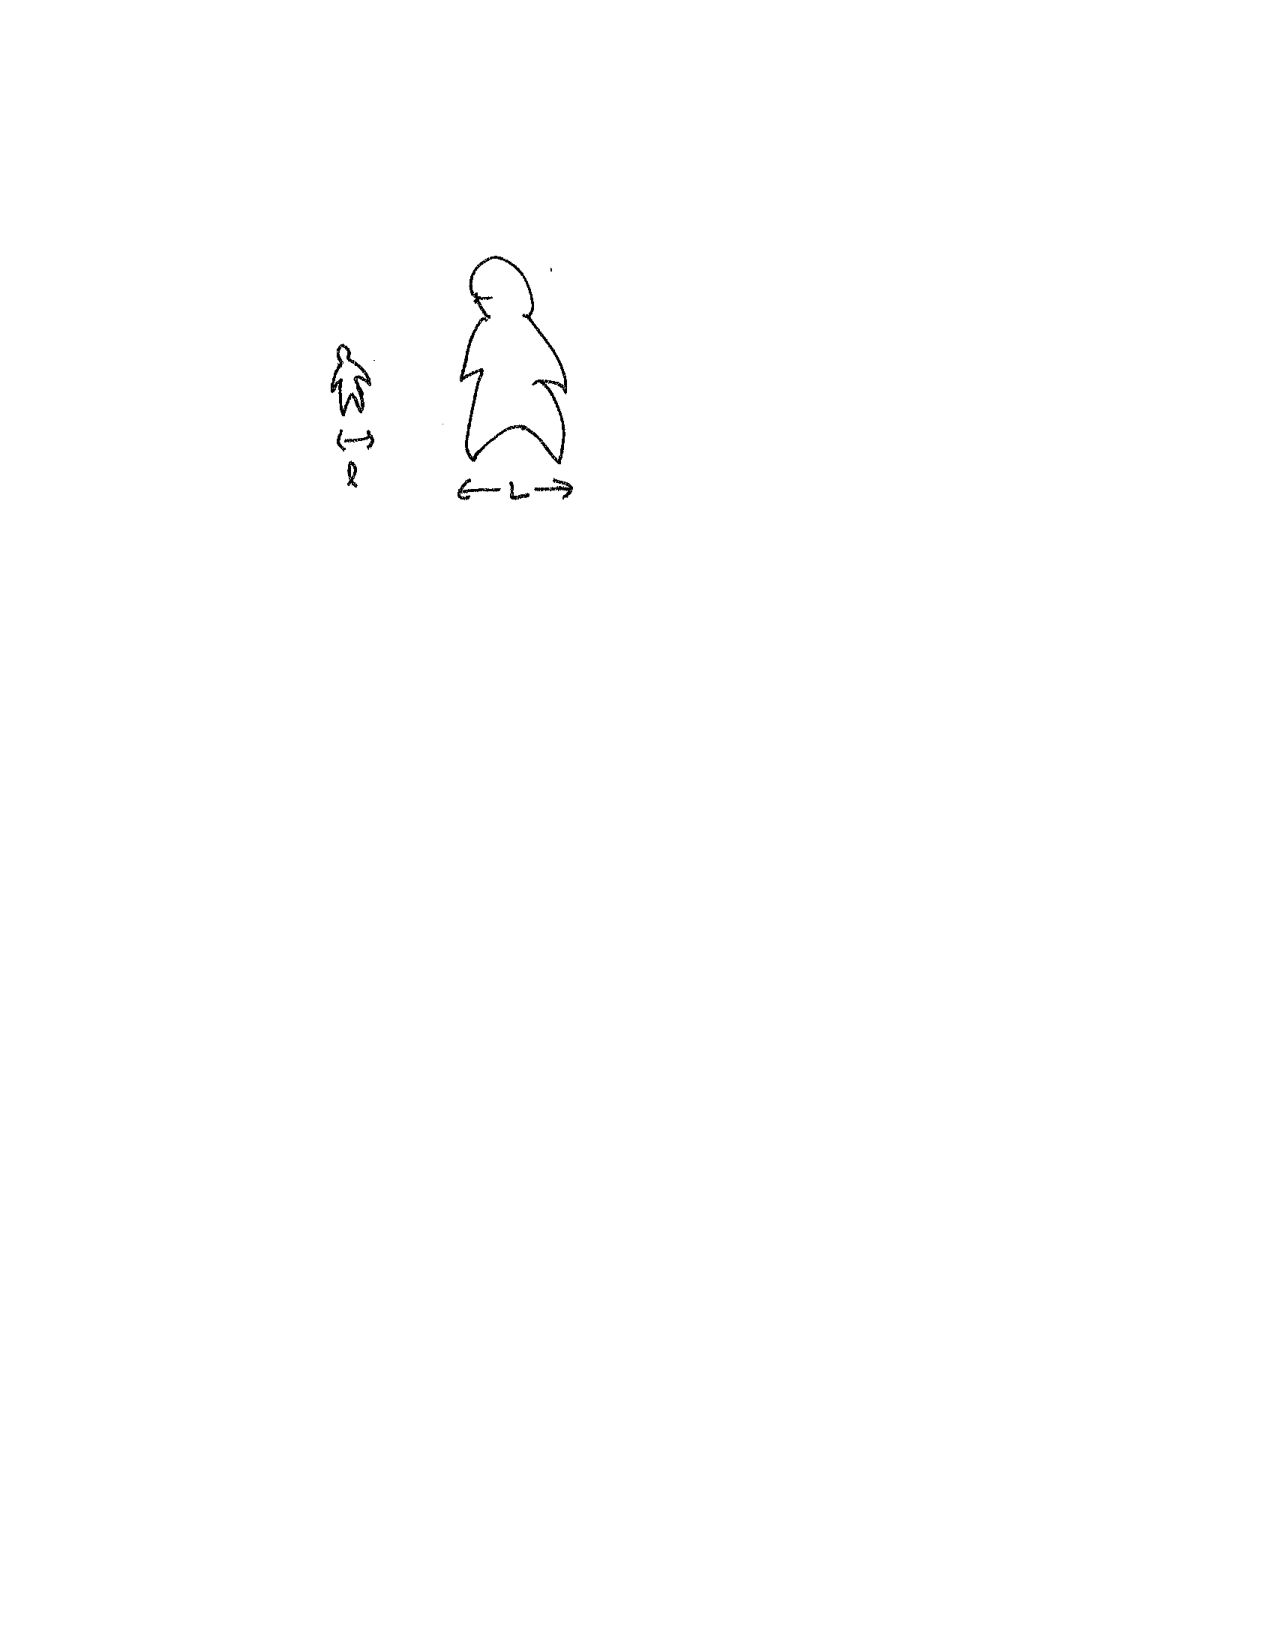
\includegraphics[width=.4\textwidth]{figures/lec01_allometry.pdf}
% \end{center}

\begin{exercise}
If both people exercised at the same rate, which one loses more absolute weight? By how much? Let us assume that weight loss is primarily from the conversion of organic molecules into carbon dioxide. 
\end{exercise}

\begin{exercise}
David Hu won his first IgNobel prize for determining that mammals take about 21 seconds to urinate, largely independently of their size\footnote{I learned about this in his excellent popular science book, \emph{How To Walk on Water and Climb Up Walls}.}. Can you use dimensional analysis to argue why this would be the case? It may be helpful to refer to the paper\sidecite{doi:10.1073/pnas.1402289111}. As you read it, figure out which terms are negligible (and in what limits), identify the assumptions of the mathematical model (scaling of the bladder and urethra), and prove the approximate scaling relation. Make a note to yourself of which steps were non-trivial and where one may have naively mis-modeled the system. By the way, David Hu won a second IgNobel prize for understanding wombats' cubical poop.
\end{exercise}

The above exercise on mammalian urination is a good example of \emph{modeling}.\index{model} As physicists, we must identify and make a mathematical model for the most salient features of a problem. We must also be able to quantify the error from neglecting sub-leading contributions. As a rough model for scaling purposes, we can ignore viscosity and surface tension effects on human-sized mammals. For much smaller mammals, these effects become larger---the authors of the study note that mice tend to urinate droplets---in which case one can ignore the `inertial' $\frac{1}{2} \rho v^2$ term in Bernoulli's equation. For human-sized mammals, we may assume that steady state urination is given by Bernoulli's equation:
\begin{align}
  P + \rho g h = \frac{1}{2}\rho v^2 \ ,
\end{align}
where $P$ is the pressure from the bladder, $h$ is the column height of the urethra, $\rho$ is the mass density of urine, and $v$ is the velocity of the urine at the end of the urethra. Let us simplify to the condition where urination is purely driven by gravity---that is, the bladder does not exert any additional pressure, $P=0$. You can now show that the total urination time scales like the mass of the mammal to the one-sixth power, $\tau \sim M^{1/6}$. That is, the urination time has a very weak scaling dependence on how massive the mammal is.

\begin{exercise}
In August 2021, Ezra Klein interviewed Dr.~C\'eline Goudner about the \acro{COVID-19} variant.~\sidecite{klein_2021} In the interview, Klein cited the statement that the Delta variant has $\mathcal O(1000)$ times the viral load than prior \acro{COVID} strains. Goudner then interprets this in the following way: if the \acro{CDC} defined `close contact' for prior strains as 15 minutes of being indoors with an infected invdividual without a mask, then the equivalent `close contact' time for the Delta variant is around \emph{one second}. What scaling assumptions go into that estimate? Some of these assumptions are not obvious to me: for example, parts of the respiratory have a fractal-like structure that would lead me to suspect fractal scaling dimensions for surface area. \acro{Remark}: Just because you know dimensional analysis, that does not make you a medical, healthcare, or public policy expert.\footnote{Early in the \acro{COVID-19} pandemic, many physicists became armchair  modelers of epidemics. Some of this was driven by hubris about our mathematical intuition. Many of the physicists lost interest when their models aligned poorly with what actually happened.} 
\end{exercise}

The following exercises draw from an article by Nicole Meyer-Verneta and Jean-Pierre Rospars in the American Journal of Physics\sidecite{doi:10.1119/1.4917310} and the references therein.
 \begin{exercise}
 Estimate the expected velocity of an All Terrain Armored Transport (\acro{AT}-\acro{AT})\footnote{\url{https://starwars.fandom.com/wiki/All_Terrain_Armored_Transport}} of characteristic height $L$. You can assume that the walking behavior is based on a pendulum. \acro{Answer}: $v \sim \sqrt{Lg}/2\pi$.
 \end{exercise}

 \begin{exercise}
 Based on the density $\rho$, the force-per-cross-sectional area $\sigma$, and the maximum rate of energy consumption per unit mass $b$, one may estimate the `sprint' velocity of an animal of length $L$. This sprint velocity is conveniently described with respect to the dimensionless `body lengths per time,' $v_\text{spr}/L$.

Remarkably, for over 20 orders of magnitude in animal length $L$, the value of $v_\text{spr}/L$ is within an order of magnitude of 10/sec:
% \begin{center}
%  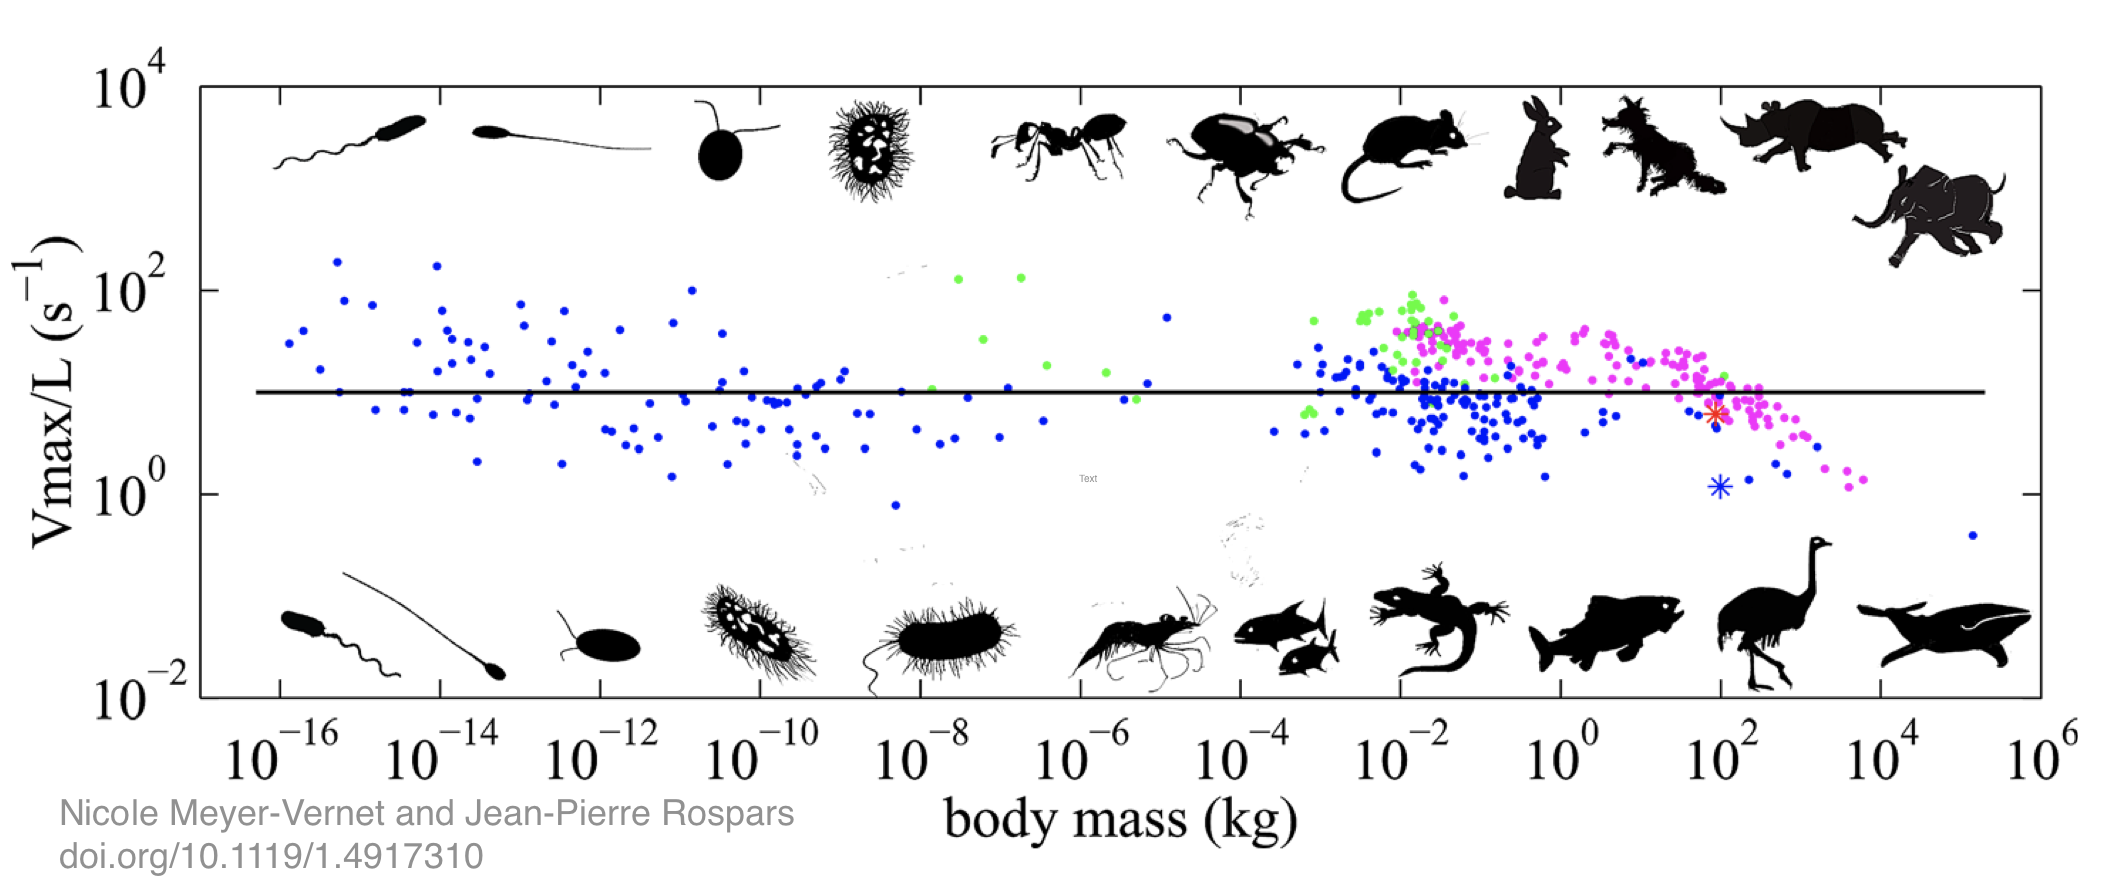
\includegraphics[width=.7\textwidth]{figures/allometry_meyer-verneta.png}
% \end{center}
\textfig[1]{figures/allometry_meyer-verneta.png}{Image from Meyer-Verneta and Rospars.~\cite{doi:10.1119/1.4917310}}{fig:allometry_meyer-verneta}


Argue from dimensional analysis that $v_\text{spr}/L \sim b\rho/\sigma$. (This is the easy part.) It turns out that there are simple physical principles for each of these terms to be roughly constant for all life on Earth (this is the more subtle part); see the article for a discussion.
\end{exercise}

\begin{exercise}
The height of trees. How does the maximum height of a tree, $L$ scale with the diameter of its cross section, $d$? For an argument that $L\sim d^{3/2}$, see Thomas McMahon's article ``The Mechanical Design of Trees'' in \emph{Scientific American} volume 233 (1975)\footnote{\url{https://www.jstor.org/stable/24949846}}. McMahon was the first to propose a physical explanation for the observed scaling law that the metabolic rate of an animal scales like the characteristic size to the 3/4 power. A nice bibliography of his work can be found in \emph{Annual Review of Biomedical Engineering}.~\sidecite{doi:10.1146/annurev.bioeng.3.1.0}
\end{exercise}


\part{Linear Algebra}

\chapter{Finite-Dimensional Linear Algebra}

\section{Yet another review of linear algebra}

Linear algebra is part of our physics \acro{DNA}. So why should we patronize ourselves with yet another review of linear algebra?
%
We want to understand Green’s functions as a matrix inverse. The `matrix' in question is the differential operator $\mathcal O$ in \eqref{eq:greens:function:equation}.
%
The identification boils down to the following:
\begin{align}
  \text{differential operator}
  &=
  \infty\text{-dimensional matrix} \ .
\end{align}
This is a poetic equal sign; for example, not every infinite dimensional matrix is a differential operator.\footnote{But by causality and locality these are the ones we care about in physics.} You may know matrices as a block of numbers that act on columns of numbers---\emph{vectors}---to produce another vector.
If differential operators are matrices, are vectors on which they act? These matrices act on a space of functions, which turns out to be a vector space:
\begin{align}
  \text{function space} &= \infty\text{-dimensional vector space} \ .
\end{align}
Again, the equal sign is poetic. 
Do not be intimidated by terminology like \emph{function space}; this is just an abstract place where functions live. Just recall back to your intuition from \acro{3D} Euclidean vector space, $\mathbb{R}^3$: any 3-vector $\vec{v}$ lives in the vector space $\mathbb{R}^3$. If we transform $\vec{v}$ by a linear transformation ${A}$, you get a new vector  $\vec{w} = {A}\vec{v} \in \mathbb{R}^3$ that is also in the vector space.

%
Weird things can happen when we extend our intuition from finite things to infinite things\footnote{For example, the Hilbert Hotel puzzle.}, but for this course we try to draw as much intuition as we can from finite dimensional linear algebra to apply it to infinite dimensional function spaces.



\section{What is Linear?}

A function\index{function}, $f(x)$, takes some kind of input $x$ and produces some kind of output. When the inputs and outputs are real numbers, $x,f(x)\in \mathbbm{R}$, then we can plot this relation between inputs and outputs on the $\mathbbm{R}^2$ by the mapping $(x,f(x))$. The curve $f(x)$ is the set of all points $(x,y) \in \mathbbm{R}^2$ such that $y=f(x)$. Said in yet another way, $y=f(x)$ is a constraint on $\mathbbm{R}^2$ that slices it into a one-dimensional subspace. To emphasize that $f$ takes in real numbers and spits out real numbers, we can write $f: \mathbbm{R}\to\mathbbm{R}$.

Before we end up getting too pedantic about what a curve is, recall that even children can tell you that the equation $f(x) = mx+b$ defines a line in the two dimensional plane. In this relation, $m$ is the slope and $b$ is the intercept of the line with the $y$-axis. We must be more restrictive: we set $b=0$ and impose that a linear relation between two numbers $x$ and $f(x)$ takes the form $f(x)=mx$. 

The reason for our apparent pedantry is to generalize the definition of {linearity} to extend beyond the picture of curves on $\mathbbm{R}^2$. A relation $f(x)$ is linear if the following are true:
\begin{align}
  f(\alpha x) &= \alpha f(x)\\
  f(x+y) &= f(x) + f(y) \ .
\end{align}
We assume that $x$ and $y$ are two objects of the same type, and $\alpha$ is simply some number.
\begin{exercise}
Confirm that $f(x)=mx$ is a linear function between real numbers for any value of $m\in \mathbbm{R}$.
\end{exercise}
We can state this all more formally. Suppose there is some collection of objects that we call $V$. Let $x$ and $y$ be two such objects: $x,y\in V$. Further, let $\alpha$ and $\beta$ be two numbers: $\alpha,\beta\in\mathbbm{R}$. Then a function $f:V\to W$ is \textbf{linear}\index{linear} if and only if\footnote{One can also write ``$\Leftrightarrow$'' to mean `if and only if.'}
\begin{align}
  f(\alpha x + \beta y) = \alpha f(x)+\beta f(y)
  \label{eq:def:linear}
\end{align}
Let us dissect this a bit. We stated that $x$ and $y$ have to be the same type of object, members of the class $V$. This echoes our discussion of dimensional analysis: if $x$ are apples and $y$ are Pokemon, then $2.5x+7y$ is nonsensical and so any function of such an object is nonsensical. We defined $\alpha$ and $\beta$ to be numbers\footnote{More generally, these are elements of a \textbf{field}: sets of objects with addition and multiplication defined.}: these just count how many objects in $V$ are being fed into our function. For now we assume that these are real numbers, but we will soon generalize to complex numbers. 

We wrote $f:V\to W$, which means that the output of the function $f(x)$ is an object of class $W$. In our toy example $f(x)=mx$, $V=W=\mathbbm{R}$. In general, $W$ and $V$ could be two totally different classes of objects. $W$ could be real numbers, something with units, a mathematical object with more structure, or any other class of objects. No matter what $V$ and $W$ are, the relation \eqref{eq:def:linear} tells us when a function is linear. 

\begin{example}
Let $f$ be a function that maps angles $\theta$ to rotation matrices,
\begin{align}
  R(\theta) = 
  \begin{pmatrix}
    \phantom{+}\cos\theta & \phantom{+}\sin\theta \\
    -\sin\theta & \phantom{+}\cos\theta
  \end{pmatrix} \ .
\end{align}
This map is not linear because
\begin{align}
  R(\theta_1 + \theta_2) \neq R(\theta_1) + R(\theta_2) \ ,
\end{align}
as you can check for the trivial case of $\theta_1 = \theta_2 = 0$.
\end{example}
\begin{exercise}
Let $f$ be a function that maps driving speed to the probability of being pulled over by the police or highway patrol. Explain why $f$ cannot be linear.
\end{exercise}

We can diagnose the linearity of a function, even when that function inputs and outputs objects that are more general than simply numbers. Thus far, we have been rather coy what it means to be an ``object in class $V$.'' This leads us to the notion of a vector space. 

\section{Vectors and Vector Spaces}

For our purposes in this course, we consider functions of \textbf{vectors}. Not all objects of interest are vectors, for example, coordinates are decidedly not vectors. The term \emph{position vector} is thus a faux pas.\footnote{Mathematicians chuckle at freshman physics textbooks.} On the contrary, infinitesimal differences of coordinates are vectors called \textbf{tangent vectors}. So what are vectors and vector spaces?

We focus on an imprecise, but physically intuitive working definition. For those who prefer a more mathematical discussion that is still tied to physical intuition, see \emph{Geometry, Topology, and Physics} by Nakahara.\sidecite{Nakahara:206619} A \textbf{vector}\index{vector} is an element of a vector space. That is, a \textbf{vector space}\index{vector space} is the `complete' collection of a given type of vector. 

We have already assumed that you can add vectors and rescale them by numbers; that is, we can take \textbf{linear combinations}\index{linear combination} of vectors. The assumption is implicit in our definition of linearity, \eqref{eq:def:linear}. Let $\vec{v}$ and $\vec{w}$ be any two vectors in the vector space $V$; we write this as $\vec{v},\vec{w}\in V$. Further, let $\alpha, \beta$ be numbers. We have the following rules:
\begin{itemize}
  \item The sum $\alpha\vec v + \beta\vec w$ is a vector in $V$. 
  \item The zero vector $\vec 0$ is a vector in $V$ such that $\vec 0 + \vec v = \vec v$. 
\end{itemize}
Formally there are other rules, but you probably already assumed them.\footnote{Please refer to your favorite linear algebra book.} These include the fact that vector addition is commutative, $\vec v + \vec w = \vec w + \vec v$, and associative, $(\vec v + \vec w) + \vec u = \vec v + (\vec w + \vec u)$. 
\begin{example}
The existence of a meaningful zero vector is one example why `position space' or coordinate space is not a vector space. The zero vector $\vec 0$ is the one that leaves other vectors unchanged upon addition: $\vec 0 + \vec x = \vec x$. Clearly this depends on the coordinate system and violates our intuition that physics should be independent of the choice of coordinates. Further, the notion of `adding positions' is physically nonsensical. On the contrary, differences of positions $\Delta{x} = \vec{x}_1-\vec{x}_2$ \emph{are} meaningful. For example, the force between two non-relativistic point particles depends the vector that is the difference between the particle positions.
\end{example}

\begin{exercise}\label{ex:color:space} \textbf{Color Space}. Colors for digital media have many representations. One popular representation is \acro{RGB} where the intensity of red, green, and blue components are specified. For example, $(25,174,40)$ is a pleasant shade of green. This triplet of numbers certainly looks like a vector: it is an ordered collection of numbers. Is the space of \acro{RGB} colors a vector space? \emph{Answer: no. Make a list of reasons why.} Like all meaningful questions, this rabbit hole runs deep; for example, see articles on the geometry of colors~\sidecite{weinberg1976geometry} or the overlapping sciences of physics and neurological perception of color~\sidecite{Logvinenko:2022}.
\end{exercise}

\section{Notation for Vectors}
\label{sec:vector:notation}

Physicists use a few different notations for vectors depending on the context. In these notes we also use whichever notation is most convenient for the task and we are not ashamed to change notation as needed. Students should be nimble to be able to make use of different notations.\footnote{As a student I was once very because a textbook introduced the notation $\overleftrightarrow{\partial}$. Only much later would I come to appreciate the perspicacity of that symbol.} It is absolutely critical that even though we can refer to a mathematical object with different notation, the underlying idea is the same. This insight is the key to never getting lost in the forest of special functions (Bessel, Legendre, spherical harmonics, etc.) that appear in physics.

\subsection{Bold/over-arrow notation} Thus far we refer to vectors with a boldfaced and italicized symbol,\footnote{See \acro{ISO 80000-2:2019} from the International Organization for Standardization.} $\vec{v}$. For the author this is a comfortable and familiar notation from school. On the board in a classroom, we sometimes write the vector with an underline $\underline{v}$ since boldfaced can be difficult to write freehand. A related notation uses arrows, $\overrightarrow{v}$. %Tensor $\tensor{T}$. ISO 80000-2:2019

\subsection{Ket notation} Another popular notation in physics is the bra--ket notation. Vectors are kets, $\ket{v}$. We we review below, there are also `row vectors' that we call bras, $\bra{w}$. This is all a tongue-in-cheek joke because you can combine a bra and a ket to form a \emph{braket}, $\langle w \,|\, v\rangle$, which we identify as the inner product (dot product) of two vectors $\langle w, v\rangle = \vec{w}\cdot\vec{v}$. 

\subsection{Index notation} A common metaphorical extension\footnote{\url{https://en.wikipedia.org/wiki/Metaphorical_extension}} in physics is the notation $v^i$. Technically, $v^i$ refers to the $i^\text{th}$ component of the vector $\vec{v}$.\footnote{$i^\text{th}$ component with respect to what? See the following section on basis vectors.} However, since physicists often write their equations component-wise, we often slip into the shorthand of using $v^i$ to mean either a given component or the entire vector. The appropriate meaning is usually clear from context. 

\subsection{Unadorned notation} We identify functions as vectors in an infinite dimensional space. In this case, it is often sufficient to avoid any additional adornment, so we write a function as $f$. The analog of a component of a vector, $v^i$, is the function at a point, $f(x)$.


\section{Basis Vectors}



The number of vectors in a vector space is formally infinite. If $\vec v$ is a vector, then so is $2v$ and $3v$, not to mention $0.999\vec{v}$, ad nauseum. Fortunately we can pick a standard set of reference vectors and define any other vector with respect to those reference vectors. We call those reference vectors \textbf{basis vectors} $\hat{\vec{e}}_{(i)}$ and the entire set a \textbf{basis}\index{basis} for the vector space.\footnote{Please humor the unusual notation with a lower index in parenthesis. We explain this unusual choice in Section~\ref{sec:indices}.} We may express any vector $\vec v$ in the vector space as a linear combination of basis vectors:
\begin{align}
  \vec{v} = \sum_i v^i\hat{\vec{e}}_{(i)} \ .
\end{align}
\begin{example}
In two dimensional Euclidean space, $\mathbbm{R}^2$ we have a canonical basis
\begin{align}
 \hat{\vec{e}}_{(1)} \equiv 
  \begin{pmatrix}
    1\\0
  \end{pmatrix}
  &&
 \hat{\vec{e}}_{(2)} \equiv 
  \begin{pmatrix}
    0\\1
  \end{pmatrix} \ .
\end{align}
\emph{Canonical} is just a fancy way to say \emph{the obvious choice}. The first basis vector points in the $x$ direction, the cond points in the $y$ direction. We can thus represent a vector $\vec{v}$ as a linear combination,
\begin{align}
  \vec{v} = 
  \begin{pmatrix}
    v^1 \\ v^2
  \end{pmatrix}
  =
  v^1\hat{\vec{e}}_{(1)} + v^2\hat{\vec{e}}_{(2)} \ .
\end{align}
We could have defined a different basis, for example
\begin{align}
 \hat{\vec{e}}_{(1)}' \equiv 
  \frac{1}{\sqrt{2}}
  \begin{pmatrix}
    1\\1
  \end{pmatrix}
  &&
 \hat{\vec{e}}_{(2)}' \equiv 
  \frac{1}{\sqrt{2}}
  \begin{pmatrix}
    \phantom{+}1\\-1
  \end{pmatrix} \ .
\end{align}
In this primed basis the vector $\vec{v}$ would have different components,
\begin{align}
  \vec{v} = v'^1\hat{\vec{e}}_{(1)}' + v'^2\hat{\vec{e}}_{(2)}' \ ,
\end{align}
where clearly $v'^i \neq v^i$.
\end{example}
\begin{exercise}
Suppose $v^1 = 3$ and $v^2 = -4.5$ in the unprimed basis from the example above. Find the corresponding primed components $v'^1$ and $v'^2$. You do not have to do this in any fancy systematic way. \emph{Suggestion}: just draw the vectors on $\mathbbm{R}^2$. You do not often get to do this, especially with more abstract vectors. But when you can do something the simple way, you should do it that way and then think about how to generalize `the simple way.'
\end{exercise}

The number of basis vectors required to describe any vector is called the \textbf{dimension}\index{dimension} of the vector space. The dimension of $\mathbbm{R}^2$ is two. If you specify fewer basis vectors than the dimension of the vector space, then there are vectors that you cannot describe. If you specify more basis vectors than the dimension of the vector space, then there is not a unique way to specify the vector components.\footnote{\emph{Then shalt thou count to three, no more, no less. Three shall be the number thou shalt count, and the number of the counting shall be three. Four shalt thou not count, neither count thou two, excepting that thou then proceed to three. Five is right out.} (\emph{Monty Python \& The Holy Grail}, 1975)}
\begin{example}
In $\mathbbm{R}^2$, suppose we specified \emph{three} basis vectors,
\begin{align}
 \hat{\vec{e}}_{(1)} \equiv 
  \begin{pmatrix}
    1\\0
  \end{pmatrix}
  &&
 \hat{\vec{e}}_{(2)} \equiv 
  \begin{pmatrix}
    0\\1
  \end{pmatrix} 
  &&
 \hat{\vec{e}}_{(3)} \equiv 
  \frac{-1}{\sqrt{2}}
  \begin{pmatrix}
    1\\1
  \end{pmatrix}
  \ .
\end{align}
The vector $\vec{v} =\hat{\vec{e}}_{(1)} +\hat{\vec{e}}_{(2)}$ can equivalently be written as $\vec{v} = -\sqrt{2}\vec{e}_{(3)}$.
\end{example}
\begin{exercise}
In the example above, write $\vec{v}$ with respect to the three basis vectors in a way that has not yet been specified. Repeat this exercise until it is obvious that there are an infinite number of ways of writing $\vec{v}$ with respect to the three basis vectors. Contrast this to the case where we restrict to any pair of the basis vectors, in which case the components of $\vec{v}$ are unique.
\end{exercise}

\section{Nice basis vectors}
\label{sec:nice:basis}

You have likely been trained to \emph{assume} that a basis is \emph{nice}, following the notion of assumed \emph{niceness}\footnote{Section~\ref{sec:niceness}.} in physics. As we move towards abstract vector spaces, it is worth explicitly stating these assumptions so that we can make a note of where they may break and what other mathematical structure we need to define them. The two assumptions are linear independence and orthonormality.

\subsection{Linear independence}

Two vectors $\vec{v}$ and $\vec{w}$ are \textbf{linearly independent}\index{linear independence} if they are not proportional to each other: $\vec{v} \neq \alpha \vec{w}$ for any number $\alpha$. The basis vectors for any reasonable basis are linearly independent---any given basis vector $\vec{e}_{(i)}$ cannot be written as a linear combination of the other basis vectors:
\begin{align}
\hat{\vec{e}}_{(i)} \neq \sum_{i\neq j}\hat{\vec{e}}_{(j)} \ ,
\end{align}
where the sum is over all basis vectors $\vec{e}_{(j)}$ except the $i^\text{th}$ basis vector. It should be obvious\footnote{In the sense of Section~\ref{sec:obvious}.} that a proposed basis with a linearly dependent basis vector
\begin{enumerate}
  \item Does not uniquely define the components of some vectors $\vec{v}$ in the vector space.
  \item Either has more basis vectors than the dimension of the space, or there are vectors in the space that cannot be described by the basis.
\end{enumerate}
Thus every basis vector in any reasonable basis is linearly independent from the other basis vectors.

\subsection{Orthonormality}

Okay, this is actually two different conditions: orthogonal and normal. The basis vectors of a nice basis are \emph{orthogonal} to every other basis vector and \emph{normalized} to have unit length. \textbf{Orthogonal} means that the vectors are perpendicular\index{orthogonal}. 

\emph{Eh...} then what do we mean by \emph{perpendicular}? We certainly have some notion of two directions being perpendicular from everyday life: north is perpendicular to west because if we move five steps north we are stationary in the east--west direction. But how do we define this mathematically? In fact, while we are at it: how do we define `unit length' with respect to these vectors?\footnote{From a physics perspective: in what units?} 

\begin{example}
Orthogonality and linear independence are related but are not the same. Orthogonal vectors are linearly independent, but linear independence does not imply orthogonality. For example, consider the basis of $\mathbbm{R}^2$:
\begin{align}
 \hat{\vec{e}}_{(1)} \equiv 
  \begin{pmatrix}
    1\\0
  \end{pmatrix}
  &&
 \hat{\vec{e}}_{(2)} \equiv 
  \begin{pmatrix}
    1\\1
  \end{pmatrix} 
  \label{eq:nice:basis:eg:e1e2}
  \ .
\end{align}
These vectors are obviously linearly independent. Assuming the usual Euclidean inner product, the are also \emph{not} orthogonal. The observant student will notice that linear independence does not require one to define an inner product, whereas orthogonality is only defined with respect to some inner product.
\end{example}
\begin{exercise}
Let $\vec{v}$ be the vector that is pointing in the $\hat{\vec{x}}$ direction of $\mathbbm{R}^2$.  What are the components of $\vec{v}$ with respect to the basis in \eqref{eq:nice:basis:eg:e1e2}? Similarly, let $\vec{w}$ be the vector that is pointing in the $\hat{\vec{y}}$ direction of $\mathbbm{R}^2$. What are the components of $\vec{w}$ with respect to the basis in \eqref{eq:nice:basis:eg:e1e2}?
\end{exercise}
Unlike linear independence, orthonormality is not a strictly necessary condition for having a basis---though it is hard to imagine a scenario where one would \emph{not} use an orthonormal basis. However, the notions of orthogonality and normalization depend on \emph{additional} mathematical structure that we have to impose/assume/invent for our vector space. Formally, we say that we promote the vector space to a \textbf{metric space}\index{metric space}. The additional structure that we define is a machine that takes two vectors and tells us something about the `distance' between them. We call this machine the \textbf{metric}\index{metric}, \textbf{inner product}\index{inner product}, or \textbf{dot product}\index{dot product}; each phrase refers to the same thing. Once we have a metric, the Gram--Schmidt procedure assures us that we can construct an orthonormal basis from a linearly independent basis, see Exercise~\ref{ex:gram:schmidt}. 


At this point we should take a deep breath and state explicitly that we’ve been assuming an orthonormal basis. In this course we will continue to use an orthonormal basis. You may object to this and say that you used to believe in orthonormal bases until you were forced to write down the gradient (or worse, the Laplacian) in spherical coordinates.

\begin{exercise}
Are polar coordinates an orthonormal basis? You can generalize this to spherical or cylindrical coordinates. Take a moment to think about this. Do vectors in polar coordinates even make sense as vectors? Do we have a sensible addition rule? These questions are unfair because they make the assumption that the vector space described by these coordinates is ``the same'' as the coordinate space. This seems perfectly innocuous until you have learned ab it differential geometry or general relativity. If this piques your interest, I encourage you to read more about this.\footnote{A good reference that presents both the physical intuition and mathematical formalism is Sean Carroll's \emph{Spacetime and Geometry}; Carroll's appendices are an excellent crash course in differential geometry.}
\end{exercise}


There are many things to be said about non-Cartesian (``curvilinear'') coordinate systems and orthonormality. None of them are particularly edifying without a full discussion. With no apologies, I make the following [perhaps perplexing] remarks, illustrated in a figure below:
\begin{enumerate}
\item There is no such thing as a `position vector.' Positions refer to some base space, whereas vectors (like differential operators) act on the tangent space at a point of that base space. 
\item A given tangent space is `nice’ and has a nice orthonormal basis. 
\item That basis may not be the same for neighboring tangent spaces (perhaps due to coordinates, perhaps due to intrinsic curvature). 
\end{enumerate}
In this course these nuances will not come up. In the rest of your life you will still have to deal with curvilinear coordinates.\footnote{There is an excellent discussion of non-coordinate bases and curvilinear coordinates in Bernard Schutz's \emph{A First Course in General Relativity}. See Chapter 5.6 (in the first edition), ``Noncoordinate bases.''} Suffice it to say that our study of function space will be nice an orthonormal. %We haven’t yet given an adequate definition of `orthonormality,’ so let's take \eqref{eq:basis:dual:vec:act:on:vec} as a working definition.

\begin{center}
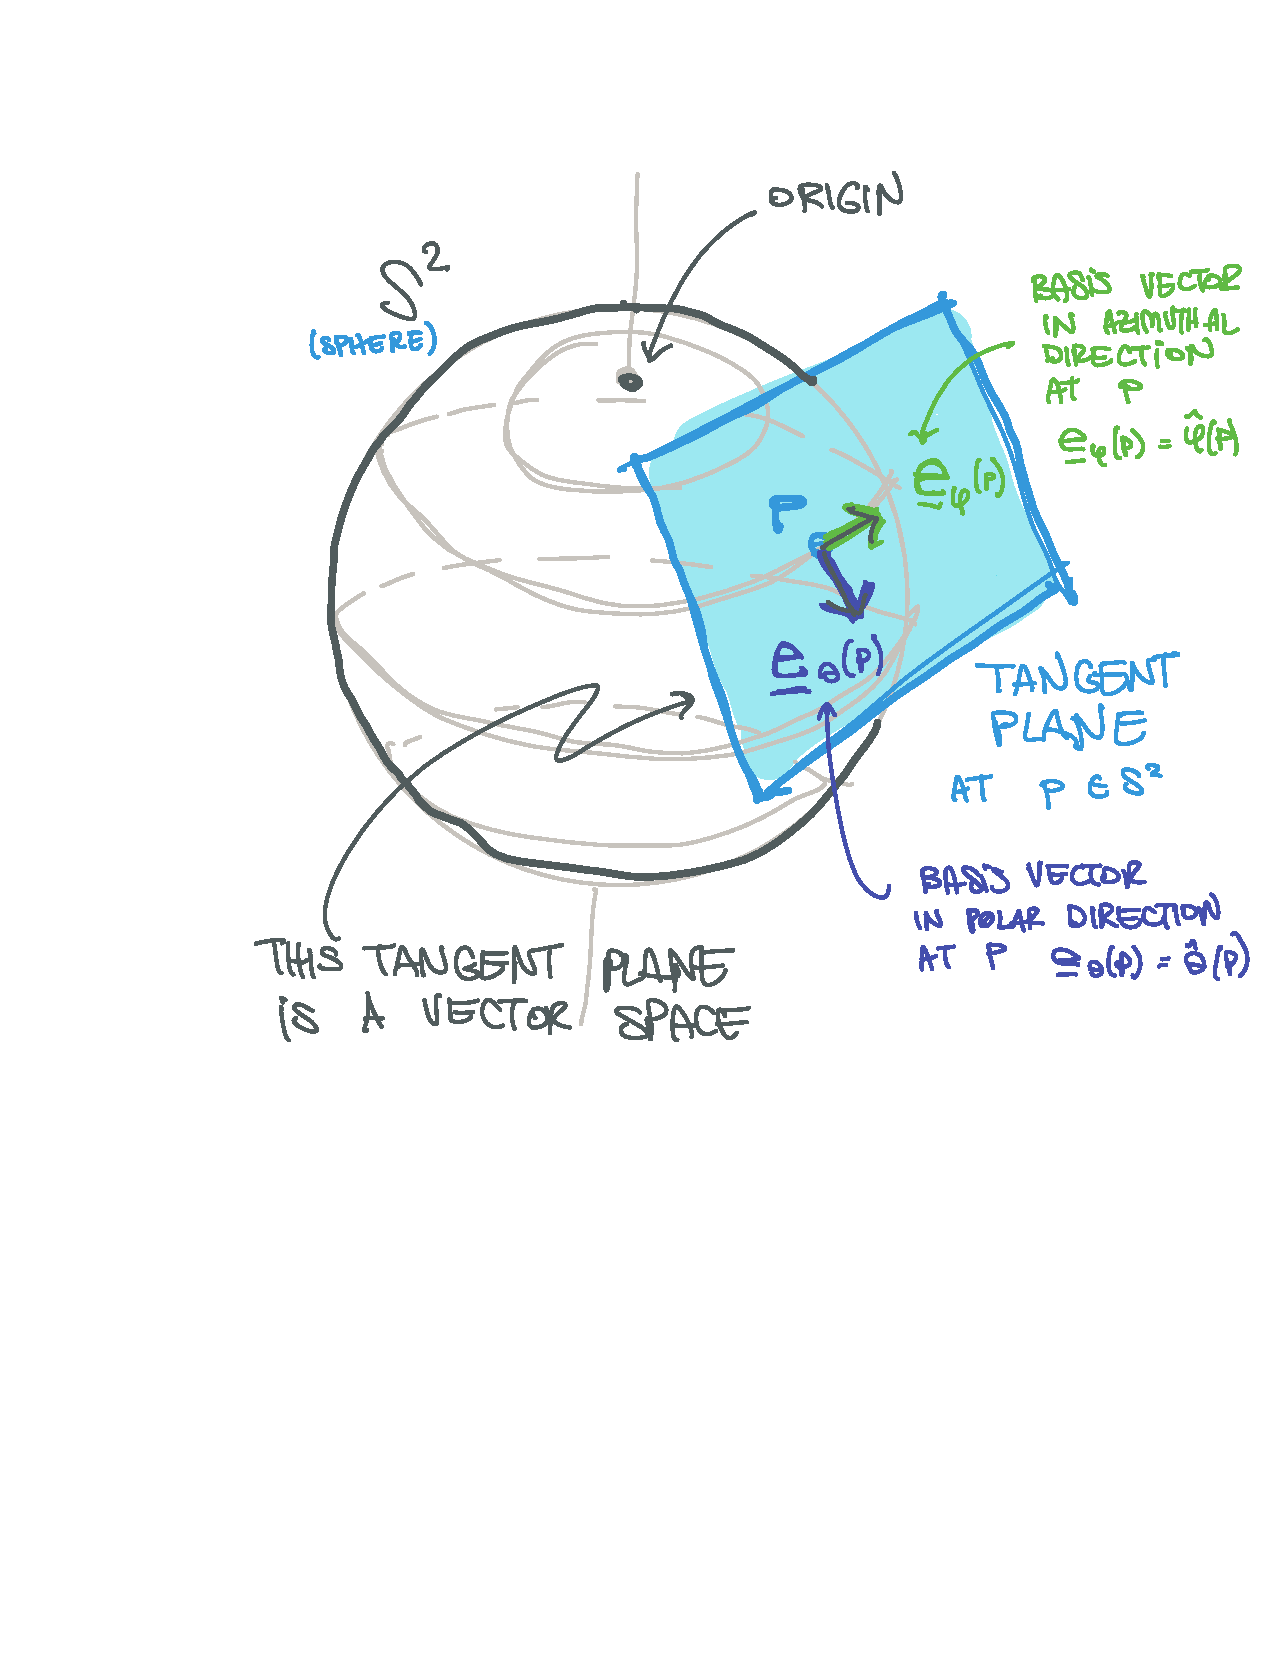
\includegraphics[width=.7\textwidth]{figures/Lec_2021_tangentS2.pdf}
\end{center}




\section{Examples of Finite-Dimensional Vector Spaces}

\subsection{Space and spacetime vectors}
There are some obvious examples of vector spaces. The one you are most used to is $\mathbbm{R}^3$, the `ordinary' (Cartesian) three-dimensional space. The components of $\vec{v}\in \mathbbm{R}^3$ are simply three real numbers $v^i$ multiplying the `obvious' basis vectors:
\begin{align}
   v^i \hat{\vec{e}}_{(i)} 
   = 
   v^1 
   \begin{pmatrix}
     1 \\ 0 \\ 0
   \end{pmatrix}
   +
   v^2 
   \begin{pmatrix}
     0 \\ 1 \\ 0
   \end{pmatrix}
   +v^3 
   \begin{pmatrix}
     0 \\ 0 \\ 1
   \end{pmatrix} \ .
 \end{align}
 We can generalized to $\mathbbm{R}^n$ with $n$ basis vectors. From special relativity you may be familiar with four-vectors with components $(p^0, p^1, p^2, p^3)$. We index starting with a zero for historical conventions, but it serves to indicate that the \emph{timelike} component $p^0$ is special. At this level, it looks like spacetime is $\mathbbm{R}^4$. An indeed, at this level that would be accurate. We will see in the next section that when we extend from a vector space to a \emph{metric space}, there is an important distinction and spacetime is in fact $\mathbbm{R}^{1,3}$.

This is a good place to remind ourselves that there is no such thing as a `position vector.' What people really mean by a position vector is the vector between some arbitrarily chosen origin and a given point on space.


There are more abstract versions of vector spaces.

\subsection{Matrices}
  The space of $2\times 2$ Hermitian\footnote{A complex matrix $A$ is Hermitian if $A^\dag = (A^\text{T})^* = A$.} matrices is a vector space with basis elements
 \begin{align}
   \mathbbm{1} &= 
   \begin{pmatrix}
     1 & 0 \\
     0 & 1 
   \end{pmatrix}
   &
   \sigma^1 &= 
   \begin{pmatrix}
     0 & 1 \\
     1 & 0 
   \end{pmatrix}
   &
   \sigma^2 &= 
   \begin{pmatrix}
     0 & -i \\
     i &  0
   \end{pmatrix}
   &
   \sigma^3 &= 
   \begin{pmatrix}
     1 & 0 \\
     0 & -1 
   \end{pmatrix} \ .
 \end{align}
 Convince yourself that you can form any Hermitian $2\time 2$ matrix out of these four basis matrices. You may recognize the familiar Pauli matrices $\sigma^i$ from quantum mechanics. 

\subsection{Quantum states}

While we have mentioned quantum mechanics, the space of quantum mechanical states is a kind of vector space. This is why the bra-ket notation that we usually learn in quantum mechanics is equally applicable to linear algebra. In fact, the big \emph{aha!} moment of the first time you learned quantum mechanics should have been when you realized that quantum mechanics is simply physicists doing linear algebra. As a bonus, quantum mechanics has primed us to already be comfortable with \emph{complex} vector spaces.

There are a few caveats. In quantum mechanics two states that differ by a phase are equivalent. This means that a state is not just a given vector $\ket\psi$ in the complex vector space, but a \emph{ray} where $\ket\psi$ is identified\footnote{We use the symbol $\cong$ to mean `identified with.'} with all rephasings, $\ket\psi \cong e^{i\theta}\ket\psi$. This identification simply means that two vectors that only differ by a phase correspond to the same quantum state: for example, they correspond to the same observable (if the states are directly observable).

\subsection{Functions}

This is a powerful idea hidden behind a trivial idea. Functions are vectors in a vector space that we call \emph{function space}\index{function space}. I am pretty sure that mathematicians do not call it that, but we use this terminology anyway.  This should be \emph{obviously} true. Consider two functions $f$ and $g$. Maybe $f(x) = x^3$ and $g(x) = x + 2$, it does not matter. Clearly you can take a linear combination of the two and the result is a function:
\begin{align}
  \alpha f(x) + \beta g(x) = \alpha x^3 + \beta x + 2\beta \ .
\end{align}
This is a totally valid function that we could call $(\alpha f + \beta g)(x)$. 

\begin{exercise}
What are some possible bases for function space?
\end{exercise}

A judicious choice of basis for function space can make our lives much easier. This is a central theme of this course and justifies the beastiary of special functions that you meet in graduate school. Let us ignore the subtleties of defining a function space for now---we get to this soon enough. The following example gives a taste of what it means to work with functions as vectors.


\begin{exercise}
%https://math.stackexchange.com/questions/942263/really-advanced-techniques-of-integration-definite-or-indefinite/943212

Here is a cute two-dimensional function space that gives us a shortcut to calculate a particular \emph{indefinite} integral.  Consider a two dimensional vector space spanned by the functions
\begin{align}
  \left|f_1\right\rangle
  &= f_1(x) = 
  e^{ax} \cos bx
  &
  \left|f_2\right\rangle
  &=
  f_2(x) = 
  e^{ax} \sin bx \ ,
\end{align}
where $a$ and $b$ are constants. Forget orthonormality or boundary conditions for this problem. The derivative $d/dx$ is a linear operator that acts on this space. Write down the derivative as a $2\times 2$ matrix in the above basis, $D$.

Invert $D$ in the usual way that you learned to invert $2\times 2$ matrices during your childhood\footnote{Stuck? Here's a life pro tip: \url{http://bfy.tw/KG2Z}}. Call this matrix $D^{-1}$. 

Now stop and think: the inverse of a derivative is an indefinite integral\footnote{Ignore the constant term.}. Thus acting with $D^{-1}$ on the vector $|f_1\rangle$ should be understood as an integral of $f_1(x)$. Show that, indeed,
\begin{align}
  D^{-1} |f_1\rangle = \int dx\, e^{ax} \cos bx \ .
\end{align}
Feel free to use \emph{Mathematica} to do the indefinite integral on the right-hand side. Pat yourself on the back if you can do it without a computer.
\end{exercise}

\subsection{More exotic examples}
 
We saw in Example~\ref{ex:color:space} that color space is almost---but not quite---a vector space. There are, however, plenty of unusual vector spaces. 

One fun example is the space of Fibbonacci sequences. These are sequences of numbers $\{x_1, x_2, x_3, \cdots \}$ such that $x_n = x_{n-1} + x_{n-2}$. You generate a Fibbonacci sequence by picking some $x_1$ and $x_2$ and determining all subsequent values using the defining rule. 
\begin{exercise}
Show that the Fibbonacci sequences form a vector space. What is the dimension of this vector space? Hint: the dimension is \emph{not infinite}.
\end{exercise}

Another example that shows up in mathematical physics is something called a \textbf{root space}. This is a space spanned by a finite number of lattice basis vectors. The space is defined so that vectors are \emph{integer} multiples of the basis vectors. Surprisingly, root space has an intimate connection to the study of continuous symmetries---the representation theory of Lie groups. 

Along these lines, you could consider the vector space of $n$-bits, $(\mathbbm{Z}_2)^n$. The bits are either zero or one and you impose modular arithmetic. 
%
You can find several other great examples by judicious Googling.\footnote{I grabbed some of these examples from \url{https://math.stackexchange.com/q/5233/1032899}.}
% fibbonacci sequences as an example
% https://math.stackexchange.com/questions/2738065/fibonacci-sequences-as-a-vector-space

%% Other great examples
% https://math.stackexchange.com/questions/5233/vivid-examples-of-vector-spaces
% simplices


\section{The metric, inner product, or dot product}

The \textbf{metric} (inner/dot product product) on a real vector space $V$ is a bilinear\footnote{This simply means linear in each argument.} map from $V\times V\to \mathbbm{R}$.\footnote{We also care about \emph{complex} vector spaces, in which case the metric is a map from $V\times V\to \mathbbm{C}$.} This means that it is a machine that takes two vectors and returns out a number. We use the metric to measure one vector with respect to another. We further impose that the metric is symmetric: it should not matter whether we measure $\vec{v}$ with respect to $\vec{w}$ or vice versa: their `overlap' should be the same. 
%
We use the angle bracket notation where $\langle \vec{v},\vec{w}\rangle$ is the inner product of two vectors $\vec{v}$ and $\vec{w}$.\footnote{This is deliberately suggestive of the ket notation for vectors, Sec.~\ref{sec:vector:notation}.}
%
Summarizing the above properties in equations:
\begin{align}
  \langle \alpha \vec{v}+\beta\vec{w}, \vec{u} \rangle &=
  \alpha \langle \vec{v},\vec{u}\rangle +
  \beta \langle \vec{w},\vec{u}\rangle 
  \\
  \langle \vec{v}, \alpha \vec{w} + \beta \vec{u} \rangle &=
  \alpha \langle \vec{v},\vec{w}\rangle +
  \beta \langle \vec{v},\vec{u}\rangle 
  \\
  \langle \vec{v},\vec{w}\rangle  &=
  \langle \vec{w},\vec{v}\rangle  \ .
\end{align}
The \textbf{norm}\index{norm} of a vector is simply its length with respect to the metric. We write the norm of a vector $\vec{v}$ as $|\vec{v}|$, or sometimes as $||\vec{v}||$ when we really want to be fancy. The norm is simply the square root of the inner product of the vector with itself:
\begin{align}
  |\vec{v}| = \sqrt{\langle \vec{v}, \vec{v}\rangle} \ .
\end{align}
Because we want lengths to make sense, we make a further requirement that any sensible metric is \emph{positive definite},\footnote{Mathematicians use the adjective \textbf{Riemannian}\index{Riemannian} to mean `positive definite' when applied to metrics. Physicists often assume that their metrics are Riemannian, with the exception of spacetime, which is semi-Riemannian... because time is funny.}
\begin{align}
  \langle \vec{v},\vec{v}\rangle > 0 
\end{align}
for any vector $\vec{v}\in V$. 
%
Both the angle bracket notation $\langle \vec v, \vec w \rangle$ and the dot product notation $\vec v \cdot \vec w$ make it clear that the metric is an operation between two vectors. There is another notation that highlights the idea of the metric as a map/function on $V\times V$:
\begin{align}
  g(\vec v, \vec w) = \langle \vec v, \vec w \rangle \ . 
\end{align}
The convention of calling the metric $g$ is common in general relativity.\footnote{Some suggest that the $g$ stands for `gravity' \url{https://hsm.stackexchange.com/questions/3435/}, see also \url{https://www.reddit.com/r/math/comments/p2i6qu/why_is_a_riemannian_metric_tensor_denoted_by_g/}.} 
% gram matrix

\begin{example} The Euclidean metric in Cartesian coordinates is the usual dot product from childhood. In $\mathbbm{R}^2$, the dot product of two vectors is $\vec{v}\cdot \vec{w} = v^1w^1 + v^2w^2$. The generalization to $\mathbbm{R}^N$ is
\begin{align}
  \langle \vec v, \vec w \rangle = g(\vec v, \vec w) = \vec v\cdot \vec w
  = \sum_{i=1}^N v^i w^i \ ,
  \label{ex:euclidean:R2:metric}
\end{align}
where $v^i$ and $w^i$ are the $i^\text{th}$ Cartesian components of the vectors $\vec v$ and $\vec w$ respectively. There are a few different ways of writing this out. 

Let $\vec v^\text{T}$ be the transpose of $\vec{v}$. We do not want to dwell on what this means (see below), but suffice it to say that if $\vec{v}$ is what a child would call a column vector, then $\vec v^\text{T}$ is what the child would call a row vector. The child may then say that the length of $\vec{v}$ is simply $$|\vec v| = \sqrt{\vec v^\text{T} \vec v}\ .$$ Observe that there is no inner product in this expression: the `row vector' $\vec v^\text{T}$ naturally acts on the column vector $\vec v$ by matrix multiplication.\footnote{As we discuss below, the row vector is a linear function from $V\to \mathbbm{R}$.} This suggests that the inner/dot product is related to
\begin{align}
  \vec v\cdot \vec w = \vec v^\text{T} \vec w \ .
\end{align}
To be fully general, we write
\begin{align}
  \vec v \cdot \vec w &\equiv \vec v^\text{T} \tens{g} \vec{w}
  &
  \tens{g} &= 
  \begin{pmatrix}
    1 & 0 \\
    0 & 1
  \end{pmatrix} \ .
  \label{eq:eg:R2:dot:product:matrix}
\end{align}
Other metrics on $\mathbbm{R}^2$ may be defined the components of the matrix $\tens{g}$. 

Yet another definition of the metric is with respect to the differential line element. For the Euclidean metric in $\mathbbm{R}^2$,
\begin{align}
  ds^2 = dx^2 + dy^2 \ .
\end{align}
This generalizes to the form
\begin{align}
  ds^2 = \sum_{i,j=1}^2 g_{ij} dx^i dx^j \ ,
  \label{eq:ds2:gij}
\end{align}
where $g_{ij}$ are the components of $\tens{g}$. Here the differentials are linear functions that take in one of the vector arguments of the metric and spit out a number.\footnote{Terms like $dx^2 = dx\otimes dx$ where the first $dx$ is a linear function of the first argument, and the second $dx$ is a linear function of the second argument.} This notation is familiar if you have studied some general relativity, but is likely completely mysterious for those with no exposure to differential geometry. Do not worry if you fare not [yet] familiar with the notation: take it as an indication that there are elegant connections between calculus and linear algebra that are waiting for you to discover them.
\end{example}

The above exercise motivates writing the inner product in \emph{tensor} notation\footnote{We deliberately postpone defining what we mean by tensor.},
\begin{align}
  g(\vec v, \vec w) \equiv \sum_{i,j} g_{ij} v^i w^j \ .
  \label{eq:metric:in:tensor:notation}
\end{align}
For the case of $\mathbbm{R}^2$ in Cartesian coordinates, \eqref{eq:metric:in:tensor:notation} matches \eqref{ex:euclidean:R2:metric} when we take the components of $g_{ij}$ to be 
\begin{align}
 g_{ij} = \delta_{ij} 
  \equiv
  \begin{cases}
  1 & \text{if } i=j \\
  0 & \text{otherwise}
  \end{cases} \ ,
\end{align}
where we define a cousin\footnote{Formally the Kronecker $\delta$ should have one upper and one lower index, as we discuss below. Our abuse of notation, however, is mostly harmless. Yes, that was a Douglas Adams reference.} of the Kronecker $\delta$.  If you are not familiar with summing over indices, please check this explicitly: \eqref{eq:metric:in:tensor:notation} has a double sum over indices $i$ and $j$, whereas \eqref{ex:euclidean:R2:metric} only has a single sum. The $\delta_{ij}$ thus collapses one of the sums by forcing one of the indices to be exactly the same as the other index. The $g_{ij}$ in \eqref{eq:metric:in:tensor:notation} is precisely the same as the one that shows up in \eqref{eq:ds2:gij}.


\begin{exercise}
Given the restriction that a metric is a bilinear function of two vectors, explain why a general $\mathbbm{R}^2$ metric may be written in the form 
\eqref{eq:eg:R2:dot:product:matrix}. Why can any bilinear function of two vectors in $\mathbbm{R}^2$ be written with respect to the four components of $\tens{g}$? What are the restrictions on the components of $\tens{g}$ given that metric is symmetric and positive definite?
\end{exercise}

\begin{example}
The two-dimensional Minkowski space metric in the standard basis is
\begin{align}
  \langle\vec{v},\vec{w}\rangle = v^0w^0 - v^1w^1 \ ,
\end{align}
where we use the standard relativistic notation that the components of a vector are labelled as
\begin{align}
  \vec v = 
  \begin{pmatrix}
    v^0 \\ v^1
  \end{pmatrix} \ ,
\end{align}
with $v^0$ being the time-like component. The generalization to $(d+1)$-dimensional Minkowski space\footnote{This is called $\mathbbm{R}^{(1,d)}$ or $\mathbbm{R}^{(d,1)}$. Occasionally we invoke spaces with more than one time dimension. Some maximally symmetric spacetimes with negative curvature---think of a Pringles potato chip---are described as surfaces in $\mathbbm{R}^{(2,d)}$.} is simply
\begin{align}
  \langle \vec{v},\vec{w}\rangle = 
  v^0w^0 - \overrightarrow{\mathbf{v}}\cdot \overrightarrow{\mathbf{w}} \ ,
  \label{eq:Minkowski:metric}
\end{align}
where $\overrightarrow{\mathbf{v}}$ are the $d$-dimensional spatial components and $\overrightarrow{\mathbf{v}}\cdot \overrightarrow{\mathbf{w}}$ represents the ordinary Euclidean inner product on space.
\end{example}

\begin{exercise}\label{ex:gram:schmidt}The \textbf{Gram--Schmidt} procedure. Given the two vectors
\begin{align}
\vec v &=
\begin{pmatrix}
     2\\0
\end{pmatrix}   
&
\vec w &=
\begin{pmatrix}
     -1\\-1
\end{pmatrix} \ ,  
\end{align}
derive an orthonormal basis on $\mathbbm{R}^2$ using the canonical\footnote{This is a fancy word that we take to mean `the usual choice.' In this case we mean the Euclidean metric.}\index{canonical} metric. You should not need instructions for how to do this, even if you do not remember the Gram--Schmidt procedure: there are only two vectors and only a small number of operations you can do with them.
\end{exercise}

\begin{exercise} The \textbf{Gram--Schmidt} procedure, generalized.
Based on the previous exercise, give instructions for how to systematically derive an orthonormal basis from a set of $d$ linearly independent vectors in a $d$-dimensional metric space. Does it matter what order you process the original $d$ vectors in this procedure?
\end{exercise}


\begin{exercise}\label{ex:polar:coordinates} Write out the Euclidean metric for polar coordinates in $\mathbbm{R}^2$, $(r,\theta)$. These are related to ordinary Cartesian coordinates by:
\begin{align}
  (x,y) &= (r\cos\theta, r\sin\theta) \ .
\end{align}
The answer is \emph{not} $\langle \vec{v},\vec{w}\rangle = v_rw_r + v_\theta w_\theta$. You know the Euclidean metric in Cartesian coordinates and you know the change of basis, so this is straightforward. 
\end{exercise}

\begin{exercise}[Surface of the sphere]
The surface of the unit sphere $S^2$ is described by two coordinates: the azimuthal angle $\theta$ (latitude) and the polar angle $\varphi$ (longitude). This is a two-dimensional surface \emph{embedded} in three-dimensional Euclidean space. One may take the three-dimensional Euclidean metric and induce a metric on the embedded $S^2$. One way to do this is to write the three $\mathbbm{R}^3$ coordinates as functions of the two $S^2$ coordinates:
\begin{align}
  x(\theta,\varphi)
  &=
  \cos\theta\,\cos\varphi
  &
  y(\theta,\varphi)
  &=
  \cos\theta\,\sin\varphi
  &
  z(\theta,\varphi)
  &=
  \sin\theta
  \ .
\end{align}
The differentials of these are now straightforward. For example,
\begin{align}
  dx & = 
  -\sin\theta\,\cos\varphi \,d\theta
  -\cos\theta\, \sin\varphi\, d\varphi \ .
\end{align}
Plug this into the Euclidean metric to derive the induced metric on $S^2$:
\begin{align}
  ds^2 
  &= 
  dx(\theta,\varphi)^2 + dy(\theta,\varphi)^2 + dz(\theta,\varphi)^2
  =
  d\theta^2 + \sin^2\theta\, d\varphi^2 \ .
  \label{eq:S2:metric}
\end{align}
\end{exercise}


\section{Inner product as a projection}

\marginfig{figures/innerprod.pdf}{Normalize two vectors $\vec{v}$ and $\vec{w}$ by dividing each by its magnitude. For example $\vec{v}/|\vec{v}|$ is a vector of unit length pointing in the same direction as $\vec{v}$. The inner product of these normalized unit vectors is the cosine of the angle between $\vec{v}$ and $\vec{w}$.}{fig:inner_prod}

The inner product has a natural geometric interpretation as the projection of one vector onto the other. By the symmetry of the metric, $\langle \vec v, \vec w \rangle = \langle \vec w, \vec v \rangle$, it does not matter which vector is being projected onto the other. This projection gives a definition of the angle, $\theta$, between two vectors:
\begin{align}
  \langle \vec v , \vec w \rangle \equiv |\vec v| |\vec w| \cos \theta \ .
\end{align}
See Fig.~\ref{fig:inner_prod}.
Writing everything explicitly in terms of the inner product:
\begin{align}
  \cos \theta = \frac{\langle \vec v , \vec w \rangle}{\sqrt{\langle \vec v , \vec v \rangle\langle \vec w , \vec w \rangle}} \ .
  \label{eq:cos:theta:def:wrt:inner:product}
\end{align}
This definition of the angle obviously matches what we expect for vectors in $\mathbbm{R}^2$. In fact, with a little bit of thought, it obviously matches what we expect for vectors in $\mathbbm{R}^d$ with $d>1$: The two vectors live in a two-dimensional subspace of $\mathbbm{R}^d$ and so the angle reduces to the $\mathbbm{R}^2$ case. What is nice about this definition is that \eqref{eq:cos:theta:def:wrt:inner:product} generalizes to \emph{any} inner product.\footnote{One place this shows up is the classification of continuous symmetry groups. \textbf{Dynkin diagrams}\index{Dynkin diagrams} indicate the `angles' between different directions in the space of symmetry transformations.} 

Given an orthonormal basis $\left\{\hat{\vec{e}}_{(i)}\right\}$,\footnote{The notation $\{\cdots\}$ refers to a set of objects. In this case we mean the set of basis vectors: $\hat{\vec{e}}_{(1)}, \hat{\vec{e}}_{(2)}, \cdots$. }, the components of a vector $\vec v$ with respect to this basis are simply the inner products:
\begin{align}
  v^i = \langle \hat{\vec{e}}_{(i)}, \vec v \rangle \ .
\end{align}
\begin{exercise}
Explain what goes wrong when the basis is not orthonormal. Give an explicit example in $\mathbbm{R}^2$. Define a non-orthonomal basis and a vector $\vec v$ with components $v^i$ with respect to the basis. Then take the inner products with the basis vectors to show that $v^i \neq \langle \hat{\vec{e}}_{(i)}, \vec v \rangle$.
\end{exercise}

Returning to our notion of a `nice basis' in Sec.~\ref{sec:nice:basis}, the orthonormality of a set of vectors is only defined with respect to a metric. A basis is orthonormal if
\begin{align}
  \langle \hat{\vec{e}}_{(i)}, \hat{\vec{e}}_{(j)} \rangle
  = \delta_{ij} 
  % \equiv
  % \begin{cases}
  % 1 & \text{if } i=j \\
  % 0 & \text{otherwise}
  % \end{cases} 
  \ .
\end{align}
% Here we have defined a cousin\footnote{Formally the Kronecker $\delta$ should have one upper and one lower index, as we discuss below. Our abuse of notation, however, is mostly harmless. Yes, that was a Douglas Adams reference.} of the Kronecker $\delta$. 
Conversely, given an orthonormal set of basis vectors the components of the metric $g_{ij}$ are,\footnote{This is sometimes callsed the \textbf{Gram matrix}} 
\begin{align}
  g_{ij} = \langle \hat{\vec{e}}_{(i)}, \hat{\vec{e}}_{(j)} \rangle \ .
\end{align}
This identification is obvious upon invoking the linearity of the inner prodcut and the expansion of any vector as a linear combination of basis vectors:
\begin{align}
  \langle \vec v, \vec w \rangle = 
  \left\langle
    \sum_i v^i \hat{\vec{e}}_{(i)},
    \sum_j w^j \hat{\vec{e}}_{(j)},
  \right\rangle
  =
  \sum_{i,j}
  v^iw^j\left\langle
     \hat{\vec{e}}_{(i)},
    \hat{\vec{e}}_{(j)},
  \right\rangle
  = 
  \sum_{i,j}
  g_{ij}v^iw^j
   \ ,
\end{align}
where the last equality identifies the metric components $g_{ij}$ in \eqref{eq:metric:in:tensor:notation}. The metric, which gives us a sense of angle and length, encodes nothing more and nothing less than the inner products of the basis vectors.

\begin{exercise}
Show that a basis is linearly independent if and only if
\begin{align}
\det\,\langle \hat{\vec{e}}_{(i)}, \hat{\vec{e}}_{(j)} \rangle \neq 0 \ .  
\end{align}
\end{exercise}
Because the metric is symmetric, it turns out\footnote{This phrase is code for ``you can prove it, but we do not prove it here.''} that one can always choose a basis where the metric is diagonal. This is tantamount to saying that there is an orthogonal basis. One can further impose that $|\det g_{ij}| = 1$ for an orthonormal basis.\footnote{The absolute value is important here because the  spacetime metric has a relative sign between timelike and spacelike components,~\eqref{eq:Minkowski:metric}.}

You may suspect that all this implies that there is always a \emph{correct} basis---or a class of correct bases---where the metric is always nice and diagonal. For many cases this is true and this is the origin of funny prefactors that show up in some of the standard mathematical expressions we use. However, there are exceptions to this. In general relativity, the statement that one can always diagonalize the metric is a \emph{local} statement. Physically this is equivalent to saying that at every point in spacetime one can chose a local inertial frame that is `free falling.' That is to say that even in a curved spacetime, at a given point you can choose coordinates where everything is Minkowski. However, the coordinates in which everything is `flat' at point $p$ do not generally match the coordinates in which everything is `flat' at point $q\neq p$. The mismatch between these coordinate systems is at the root of the mathematical structure of general relativity: it is the physical origin of the notions of connection (covariant derivative), parallel transport, and moving frames.\footnote{An excellent introduction that is grounded in physical intuition is Carroll's \emph{Spacetime and Geometry}. The appendices are a crash course in a graduate differential geometry course.}


\begin{example}
We saw that Fibbonacci sequences form a vector space. Give an example of a reasonable metric on this vector space?. Answer: a good choice is the two-dimensional Euclidean metric applied to the first two elements. When the first two elements of two Fibbonacci sequences match, then the entire sequences are identical. In fact, with this definition, the space of Fibbonacci sequences is identical (isomorphic) to $\mathbbm{R}^2$.  
\end{example}

\section{Linear functions of vectors}

Recalling our definition of linearity in \eqref{eq:def:linear}, we now focus on the class of linear functions that take in a vector and spit out a number. To say that mathematically, we consider linear functions from $V\to \mathbbm{R}$. This class of functions turns out to be significant enough to have a name. In fact, it is so significant that it has several names---and we do not always make it clear that we mean the same thing: \textbf{row vector}\index{row vector}, \textbf{bra}\index{bra}, \textbf{covariant vector}\index{covariant vector}, \textbf{one-form}\index{one-form}, \textbf{dual vector}\index{dual vector}, \textbf{covector}\index{covector}.\footnote{In japanese the prefix \emph{ko}- means `little.' That has nothing to do with the `co' in `covector,' but I recently learned about \emph{ko} in the context of the San-X characters Rillakuma and Korillakuma. The characters are delightful, but do not confuse yourself by thinking that vectors and covectors are related in the same way that Rillakuma and Korillakuma are related. It is really not even clear to me how the latter two are related.} All of these refer to the same idea of being a linear function on vectors that returns a number. By the way, there is a corresponding plurality of names for what we have thus far been calling a vector: column vector, ket\index{ket}, and \textbf{contravariant vector}\index{contravariant vector} all mean `vector.' 

The prototypical example here is a row vector. If we write a vector as a column of $N$ numbers,
\begin{align}
   \vec v = 
   \begin{pmatrix}
     v^1 \\
     \vdots \\
     v^N
   \end{pmatrix} \ ,
 \end{align}
 then a row vector $\tilde{\vec w}$ is---no surprise here---a row of $N$ numbers:
\begin{align}
  \tilde{\vec w} = 
  \begin{pmatrix}
    w_1, w_2, \cdots, w_N
  \end{pmatrix}\ ,
\end{align}
where we have very deliberately written the components with a lower index. We recall that the elementary school rule for matrix multiplication between two objects $\tilde{\vec w}$ and $\vec v$:
\begin{enumerate}
  \item Rotate the first object by $90^\circ$ in the clockwise direction. This means that $\tilde{\vec w}$ is rotated into a column of numbers.
  \item Multiply the elements of the two objects that are the same height. In this case, we multiply $w_1$ by $v^1$, $w_2$ by $v^2$, and so forth. 
  \item Sum together these multiplications: $w_1v^1 + w_2v^2 + \cdots$.
\end{enumerate}
See Fig.~\ref{rowcolmult}.
%%% 
\marginfig{figures/rowcolmult.pdf}{Multiplying a row vector and a column vector, elementary school version.}{fig:rowcolmult}
%
In this way, the row vector $\tilde{\vec w}$ acts on the column vector $\vec v$ as
\begin{align}
  \tilde{\vec w} \vec v = \sum_i w_iv^i \ ,
  \label{eq:dual:vec:act:on:vec}
\end{align}
for some numbers $w_i$. The right-hand side here is clearly a number. Furthermore, it should be clear that the right hand side depends linearly on both $\tilde{\vec w}$ \emph{and} on $\vec v$. This means if we replace $\tilde{\vec w}$ with $2 \tilde{\vec w}$, then the number on the right-hand side doubles, and similarly with $\vec v$. In fact, we can be even more explicit about the role of $\tilde{\vec w}$ as a function that takes in vectors by writing this action as $\tilde{\vec w}[\vec v]$.

\begin{exercise}
Show that the space linear functions that map $V\to \mathbbm{R}$ is also a vector space with the same dimension as $V$. We call this the \textbf{dual vector space}, $V^*$.\index{dual vector space} Two thoughts should occur to you:
\begin{enumerate}
  \item The word `dual' seems to imply that the linear functions on $V$  are somehow identical\footnote{Perhaps a more mathematical word is `isomorphic.'} to the vectors in $V$.
  \item The prior point is `obvious' from the elementary school perspective that row vectors are simply column vectors that have been written horizontally.
\end{enumerate}
\end{exercise}



\subsection{Basis row vectors}

We can define a basis of row vectors/one-forms/bras/covariant vectors analogously to the basis of vectors. In the boldface notation, we could write these as $\tilde{\vec{e}}^{(i)}$ so that a row vector $\tilde{\vec w}$ may be expanded as
\begin{align}
 \tilde{\vec w} = \sum_i w_i \tilde{\vec{e}}^{(i)} \ ,
\end{align}
where we observe the careful placement of indices. The $w_i$ are simply the components of the row vector with respect to the specified basis. These components are simply numbers. All of the \emph{row-vector-ness} of a row vector is carried in the basis row-vectors. Everything that makes a given row vector unique is specified in the components $w_i$ that specify a particular linear combination of basis row-vectors.

In principle one can choose any set of basis row vectors satisfying linear independence. Obviously we prefer to have an orthonormal basis\footnote{If you are paying close attention you notice that we have not yet defined an inner product for the row vectors. Such an inner product is necessary to define `orthonormality' on this space of row vectors.}

We underline the following point:
\begin{quote}
If you know the what the basis objects do, then you know everything about the space.
\end{quote}
Given an orthonormal basis $\left\{\hat{\vec{e}}_{(i)}\right\}$ for the vector space $V$, there is a natural choice for a nice basis for the dual vector space $V^*$ of row vectors/dual vectors/bras/covariant vectors/one-forms.\footnote{Is it clear that these are all the same things? We can then just call them dual vectors or bras.} These are the basis linear functions that satisfy:
\begin{align}
  \tilde{\vec e}^{(i)} \left[\hat{\vec{e}}_{(j)}\right] = \delta^i_j
  \equiv
  \begin{cases}
  1 &\text{if } i=j\\
  0 &\text{otherwise} \ .
  \end{cases}
  \label{eq:canonical:dual:basis}
\end{align}
We read this as a basis dual vector $\tilde{\vec e}^{(i)}$ acting\footnote{I always thought about this as Pac-Man eating the ghosts. \emph{Pac-Man} is a video game invented by Toru Iwatani for Bandai Namco in 1980. The game development started nearly the same time that---in a different part of the world---Michael Green and John Schwartz began a fruitful collaboration that would lead to the first string revolution four years later. When Green and Schwartz discovered the remarkable cancellation of anomalies in their theory, \emph{Pac-Man} had just been released on the Nintendo Entertainment System.} on a basis vector $\hat{\vec{e}}_{(j)}$.
This canonical choice of basis realizes the rule \eqref{eq:dual:vec:act:on:vec} with the coefficients $w_i$ identified as the components of $\tilde{\vec w}$.

$\delta^i_j$ is the Kronecker $\delta$\index{Kronecker delta} with one upper and one lower index. When summing over the Kronecker $\delta$ with respect to either index, it enforces that the term only contributes when the two indices match. It replaces the sum over $i$ with a fixed value $i=j$, and vice versa.

It is perhaps useful to use a slightly different notation based on Pac-Man. Rather than writing $\tilde{\vec{e}}^{(i)}$, lets write the basis dual vectors as
\begin{center}
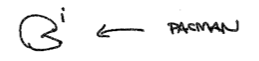
\includegraphics[width=.4\textwidth]{figures/lec05_pacman.png}
\end{center}
In this notation, the action of a basis dual vector on a basis vector is simply Pac-Man eating the basis vectors:
\begin{center}
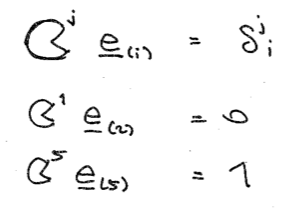
\includegraphics[width=.4\textwidth]{figures/lec05_paceats.png}
\end{center}
So we can write \eqref{eq:dual:vec:act:on:vec} as
\begin{center}
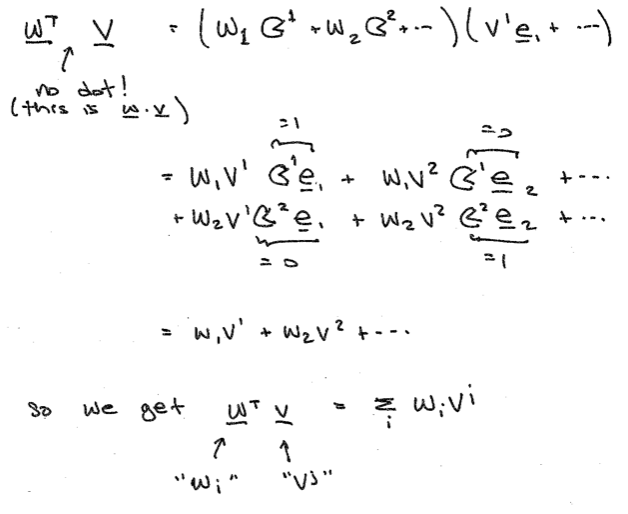
\includegraphics[width=.7\textwidth]{figures/lec05_paccontract.png}
\end{center}

\subsection{Creating dual vectors with a metric}

Let us be very clear: these dual vectors (row vectors, one-forms, bras, covariant vectors) \emph{do not require a metric}. The metric takes in two vectors and spits out a number, $V\times V\to \mathbbm{R}$. A row vector takes in a single vector and spits out a number, $V\to\mathbbm{R}$.\footnote{This is a good place to remind ourselves that eventually we replace $\mathbbm{R}$ with the complex numbers, $\mathbbm{C}$. One may further generalize to different \emph{fields}---generalizations of `numbers'.} These are two very different classes of objects. 

However, if our vector space happens to be a metric space---that is, if we happen to have a metric lying around that we care to attach to $V$---then we can use the metric to create dual vectors out of vectors. 
\begin{exercise}
If you do not already know the answer, then pause and take a moment to think how you would create a linear function from $V\to \mathbbm{R}$ given a bilinear function from $V\times V\to \mathbbm{R}$. This is a good way to check if you are parsing this information actively or if you have fallen asleep.\footnote{\emph{Inception} (2010), Christopher Nolan.} 
\end{exercise}

The idea is that we can \emph{pre-load} the metric with a vector. Pick any vector, $\vec{v}$. Now insert $\vec v$ into the first argument of the inner product, $\langle \vec v , \texttt{\textvisiblespace}\rangle$. This object now takes in a vector to fill in the second argument of the inner product and uses the machinery of the inner product to spit out a number. By the linearity of the inner product, $\langle \vec v , \texttt{\textvisiblespace}\rangle$ is a linear function from $V\to \mathbbm{R}$. This is precisely a dual vector. In fact, let us give this object a name:
\begin{align}
  \tilde{\vec v} = \langle \vec v , \texttt{\textvisiblespace}\rangle \ .
  \label{eq:tilde:v:as:transpose:metric}
\end{align}
Ta-da! We have successfully constructed a dual vector out of a vector. What are the components of this dual vector? Assuming the canonical basis for the dual space \eqref{eq:canonical:dual:basis}\footnote{This is by construction: we only have the basis of $V$ and create a basis for $V^*$ out of it.}, we can find the components of a dual vector by feeding it basis vectors:
\begin{align}
  \tilde{\vec v}\left[\hat{\vec e}_{(i)}\right]
  = 
  \sum_j v_j \tilde{\vec e}^{(j)} \left[\hat{\vec e}_{(i)}\right]
  = 
  v_j \ .
\end{align}
Applying our definition of $\tilde{\vec v}$ as a pre-loaded metric \eqref{eq:tilde:v:as:transpose:metric},
\begin{align}
\tilde{\vec v}\left[\hat{\vec e}_{(i)}\right]
= 
\sum_j v^j \langle\hat{\vec e}_{(j)},\hat{\vec e}_{(i)}\rangle  
= v^i \ .
\end{align}
From this we find that $v_j = g_{ji} v^i$, where we have used the tensor notation of the metricm \eqref{eq:metric:in:tensor:notation}. For the Euclidean metric where $g_{ji} = \delta_{ji}$ we have $v_i = v^i$: that is, the row vector has the same components as the column vector from which it was created. We now recognize that this operation of `pre-loading a metric' with a vector to create a dual vector is simply what we had been calling the \textbf{transpose}\index{transpose} of a vector:
\begin{align}
  \vec v^\text{T} = \tilde{\vec v} = \langle \vec v , \texttt{\textvisiblespace}\rangle \ .
  \label{eq:transpose:as:inner:product:preloaded}
\end{align}
There is a generalization of the transpose to complex vector spaces called the \textbf{Hermitian conjugate}, which is the combined transpose and complex conjugation.\index{Hermitian conjugate} The symbol is the dagger, $\vec{v}^\dag = \tilde{\vec v}$. If you are not sure whether a space is real or complex, you can say Hermitian conjugate to cover both cases and sound fancy.\footnote{This reminds me of people who say \emph{compote} instead of \emph{jam}.}

We recognize that if the metric is not simply $g_{ij} = \delta_{ij}$, then the components of the dual vector are different from the components of the vector.\footnote{We know that we can diagonalize the metric with an auspicious choice of basis. However, there are plenty of non-trivial diagonal metrics. Consider Minkowski space or polar coordinates.} We can appreciate the utility of the upper and lower indices: something with an upper index is a component of a vector, while something with a lower index is a component of a dual vector. We can use the metric to convert from vectors to dual vectors, and the action on the components is clear: $v_i = \sum_i g_{ij}v^j$. In other words, the metric $g_{ij}$ is a machine that can lower indices.

Please appreciate that the phrase `lower the index' is really shorthand for \emph{convert the components of a vector into the components of the associated dual vector by taking the transpose/pre-loading the metric with that vector.} It is kind of a mouthful, so we say `lower the index' as a shortcut. Sometimes we even \emph{think} about the metric as acting on the indices of the components. But this too is a mental shortcut for understanding that we are moving between elements of a vector space and linear functions on those vectors.

\subsection{Bra and Ket notation}

The utility of the bra/ket notation in quantum mechanics is now evident. A vector is written as a ket, $\vec v = \ket{v}$. A dual vectors are written as a bra, $\tilde{\vec w} = \bra{w}$. The basis bras and kets are written as follows:
\begin{align}
  \ket{v} &= v^i\ket{i} &\Leftrightarrow&&
  \vec{v} &= v^i \hat{\vec e}_{(i)}
  \\
  \bra{w} &= w_j\bra{j} &\Leftrightarrow&&
  \tilde{\vec{w}} &= w_j \tilde{\vec e}^{(j)} \ .
\end{align}
One downside of the notation is that you have to mentally remember that the basis bra $\bra{j}$ is secretly a lower index while the basis ket $\ket{i}$ is secretly an upper index. On the other hand, the notation has the feature of connecting a vector to its transpose\footnote{We should really say `Hermitian conjugate' because the bra/ket notation is most commonly used for Hilbert spaces, which are complex vector spaces.}. Given a ket $\ket{v}$, there is a natural understanding what the corresponding bra is with respect to the inner product:
\begin{align}
  \bra{v} = \langle v | \texttt{\textvisiblespace} \rangle \ ,
\end{align}
where it is understood that the action of $\bra{v}$ on $\ket{w}$ is
\begin{align}
  \bra{v}\left[\ket{w}\right] = \langle v | w\rangle = \langle v, w \rangle \ .
\end{align}
We emphasize that $\langle v | w\rangle$ is a bra acting on a ket, wheras $\langle v | w\rangle$ is the inner product of two kets.


\subsection{The form notation}

A separate notation for vectors and dual vectors is inspired by differential geometry: 
\begin{align}
  \vec{v}=v^i \hat{\vec{e}}_{(i)} &\leftrightarrow v^i \frac{\partial}{\partial x}_i
  &
  \tilde{\vec w}=w_i \tilde{\vec{e}}^{(i)} &\leftrightarrow w_i dx^i \ .
\end{align}
The notation is perplexing the first time you see it. Everything looks familiar from calculus, but is now being used in a completely unusual context. Somehow:
\begin{itemize}
   \item Partial derivatives are the basis vectors. How odd! Partial derivatives are supposed to act on functions. Evidently the elements of the vector space are linear combinations of partial derivatives. 
   \item The infinitesimal elements, for example $dx$ or $dy$, are dual vectors. This is even more strange. Based on our intuition from freshman physics, there is no sense in which an ``infinitesimal displacement'' acts on a partial derivative to spit out a number! Though it is perhaps fair to say that the linear combination of infinitesimal displacements is still an infinitesimal displacement---whatever that means.
 \end{itemize} 
 \begin{exercise}
 Confirm that the set of partial derivatives $\partial_x$, $\partial_y$, $\partial_z$ form a three-dimensional vector space. Here $\partial_x = \partial/\partial x$ and so forth. The vector space is the space of first order partial derivative operators acting on a function. This is trivial: do linear combinations of these operators live in the space? If you are caught up on ``but what are these operators acting on?'' then you are focused on the wrong thing.
 \end{exercise}
 This all implies further structure that we have not specified. The further structure is the idea of a bundle over a manifold. We give a hint of this in Chap.~\ref{chap:vector:fields}.

 Let us be clear. We are \emph{defining} the object $dx$ as a basis for linear functions acting on the vector space of partial derivatives. In this context, we call these row vectors \textbf{differential one forms}\index{differential one forms}. The action of a differential one-form on a partial derivative is
 \begin{align}
   dx^i\left[\frac{\partial}{\partial x^j}\right] \equiv \delta^i_j \ ,
 \end{align}
 which you already know from \eqref{eq:canonical:dual:basis}. The utility of this notation is illuminated in the places where differential geometry intersects with physics. We present the notation here for those who anticipate meeting this formalism in the near future: by emphasizing that this curiosity is nothing more than vectors and dual vectors, they may then focus on the ways in which this story plays out on differential manifolds.\footnote{Manifold is another fancy word for what physicists usually call space or spacetime. It is like saying \emph{pommes frites} instead of \emph{french fries}.} 
 

\section{Summation convention}

From now on we invoke the summation convention that is standard in special and general relativity:
\begin{quote}
Whenever you see exactly one upper index that is the same as exactly one lower index, there is an implied sum over that index.
\end{quote}
This is the notational equivalent of tipping at a restaurant in the United States: you are never explicitly told to tip, but it is implied that a tip for the server should added to the final bill.\sidecite{segrave2009tipping}

The summing over two indices is called \textbf{contraction}\index{contraction} of these indices. This comes from the mental shorthand of replacing (dual) vectors with their components. If we think of $\vec{v}$ as $v^i$ and $\tilde{\vec{w}}$ as $w_i$, then we can think of the action of $\tilde{\vec w}$ on $\vec v$ as a contraction of the indices of their components:
\begin{align}
  \tilde{\vec w}\vec{v} = w_i v^i = w_1v^1 + w_2v^2 + \cdots \ ,
\end{align}
where we are using the summation convention on the right hand side.
%
The summation convention comes about from the observation that there are only certain ways in which objects in linear algebra can combine. It is incredibly useful and saves several pen/pencil/chalk/keystrokes,\footnote{Nevermind the indignities of using a whiteboard.}, but leads to the common mental shorthand that an object \emph{is} its components.\footnote{A vector $\vec{v}$ is fully specified by its components $v^i$ once you agree on a basis. However, the vector is not its components. The components tell you the specific linear combination of basis vectors.}

\begin{exercise}
Which of the following is an appropriate use of the summation convention? Anything that is not appropriate is nonsense and should ideally never appear in your work.
\begin{align}
  % v^i w^k g_{ik} &= v^1w^1g_{11}+v^2w^1g_{21} + \cdots + v^1w^2g_{12} + \cdots
  % \\
  v^i w^i &= w^1 v^1 + w^2 v^2 + \cdots
  \\
  g_{ij}v^iw^i u^j &= g_{11}v^1w^1u^1 + g_{12}v^1w^1u^2 + \cdots  + g_{21}v^2w^2u^1 + \cdots \\
  g_{ii}v^iw^i &= g_{11}v^1w^1 + g_{22}v^2w^2 + \cdots 
\end{align}
Answer: these are all inappropriate. 
\end{exercise}

A few useful guidelines:
\begin{enumerate}
  \item The summation convention is a shorthand. You can start by writing (explicitly or just mentally) the full expression with a big clunky summation symbol. Then simply erase the summation. 
  \item Conversely, if you have an expression where a contraction does not make sense even when writing out the summation symbol explicitly, then the expression is probably wrong.
  \item Once you use an index, say $i$, in a contraction, \emph{never} use that index again in the same expression. This leads to confusion. We say that the contracted index is a \textbf{dummy index}\index{dummy index}. This means that it is no longer a real index because it has been summed over.\footnote{The phrase dummy index reminds me of the dummy plug system in \emph{Neon Genesis Evangelion}.}
  \item If the same index appears more than once, go directly to jail.\footnote{Do not pass go. Do not collect \$200. This is a reference to \emph{Monopoly}.}
  \item If you contract two indices of the same reflect on the questionable decisions brought you to this point.\footnote{There are some times when it is convenient to break this rule and allow contraction of same-height indices when (1) the metric is $g_{ij}=\delta_{ij}$ and (2) there is little chance of confusion.}
  \item When there is any possibility of ambiguity, explicitly say whether or not a repeated index is meant to be summed over.  
\end{enumerate}

\begin{example}
Linear transformations are linear functions that take vectors to vectors, $V\to V$. These are represented by matrices, see Sec.~\ref{sec:linear:transformations} The components of a matrix are written with an upper index (the first index) and a lower index (the second index): $A^i_{\phantom ik}$. The trace of the matrix is $A^i_{\phantom ii} = A^1_{\phantom 11} + A^2_{\phantom 22} + \cdots$. When there is no ambiguity, sometimes we write $A$ to mean the trace of $A$. This makes sense since the trace of a matrix has no indices: it is simply a number. However, this is often tons of ambiguity since there are other objects formed out of a matrix that are simply numbers, like the determinant. 

Bonus: how would you write the determinant of a matrix in terms of indices? Answer: we have not yet defined the necessary machinery to write out the determinant. What sort of machinery is missing? 
\end{example}

% Differential notation. Hints at vectors and one forms.
% linear approximation

\section{Linearity and Indices}

You should now appreciate that there is something to this whole index notation business that is intrinsically tied to the idea of linear maps.\footnote{You may also be wondering why we only care about linear maps. Let us remind ourselves that the essence of calculus is to squeeze the most out of a linear approximation to our functions.} One way of understanding this is that the point of writing indices is to treat objects as linear maps with respect to a vector space. 

\begin{exercise}
Consider a linear function $f(x)$ where $x$ is a real number. In grade school you may have learned that linear functions take the form $f(x)= ax+b$. Indeed, this equation plots to a line in the $(x,f)$ plane. Show that with our definition, a linear function $f(x)$ cannot have a constant term, $b=0$. \textsc{Hint}: $b\neq 0$ means there is some $x_0 \neq 0$ such that $f(x)=0$. That means $f(x)+f(x_0) = f(x)$. Where does this mess things up?
\end{exercise}

\begin{example}
Suppose you have a linear function in one dimension, $f(\vec{x})$. For simplicity, let $\vec{x}$ be a vector in the simple vector space, $\mathbbm{R}$. We normally think of the real numbers as, well, numbers. It should be clear that they are also the most boring vectors: sums of real numbers are real numbers, you can rescale real numbers by numbers to get a real number. 


Linearity means that 
\begin{align}
  f(\alpha \vec{x}+\beta\vec{y}) =
  \alpha f(\vec{x})+ \beta f(\vec{y}) \ .
\end{align}
The only way this is possible is if
\begin{align}
  f(\vec{x}) = a\vec{x} \ ,
\end{align}
where $a$ is some number that completely specifies the linear function $f$. In fact, $a$ is the single \emph{component} of $f$. 
\end{example}

\begin{example}
Same a the previous example, but now suppose that $\vec{x}$ is an element of the two dimensional vector space $\mathbbm{R}^2$. Let us write out the linearity condition in the column vector notation. 
\begin{align}
  f\left[
  \alpha 
  \begin{pmatrix}
    x^1 \\ x^2
  \end{pmatrix}
  + 
  \beta
  \begin{pmatrix}
    y^1 \\ y^2
  \end{pmatrix}
  \right]
  =
  \alpha f\left[
  \begin{pmatrix}
    x^1 \\ x^2
  \end{pmatrix}
  \right]
  + 
  \beta f\left[
  \begin{pmatrix}
    y^1 \\ y^2
  \end{pmatrix}
  \right] \ .
\end{align}
Consider the case $x^2 = y^2=0$. Restricting to this subspace reduces us back to the previous example, from which we deduce that
\begin{align}
  f\left[
  \begin{pmatrix}
    x^1 \\ x^2
  \end{pmatrix}
  \right]
  = a x^1 + \left(\text{independent of }x^1\right) \ ,
\end{align}
for some constant $a$.
This is the only way to satisfy linearity. By a similar argument for $x^1 = y^1 = 0$, we see that 
\begin{align}
  f\left[
  \begin{pmatrix}
    x^1 \\ x^2
  \end{pmatrix}
  \right]
  = b x^2 + \left(\text{independent of }x^2\right) \ ,
\end{align}
for some constant $b$. We know that there cannot be an overall constant term that is independent of both $x^1$ and $x^2$ since this would violate the linearity condition, see exercise above. In fact, we can change notation a bit and write $a\equiv f_1$ and $b\equiv f_2$, making the \textbf{components} of the linear function $f$ clear. We can then write the linear map as
\begin{align}
  f(\vec{x}) = f_1 x^1 + f_2 x^2 = 
  \begin{pmatrix}
    f_1 & f_2
  \end{pmatrix}
  \begin{pmatrix}
    x^1 \\ x^2
  \end{pmatrix} \ ,
\end{align}
where in the last equality we have returned to the usual grade school row-vector/column-vector notation. If we insert the basis vectors and covectors, this is simply
\begin{align}
  f(\vec{x}) &= 
  \left(f_1 \langle 1| + f_2 \langle 2|\right)
  \left(x^1|1\rangle + x^2|2\rangle\right) 
  \\
  &= 
  f_1 x^1 \langle 1|1\rangle + f_2 x^1 \langle 2|1\rangle
  f_1 x^2 \langle 1|2\rangle + f_2 x^2 \langle 2|2\rangle
  \\
  &= f_ix^i
  \ ,
\end{align}
which of course returns the same linear combination of components due to $\langle i | j\rangle = \delta^i_j$.
\end{example}

\section{Duality}

Thus far the relation between vectors and dual vectors seem a bit one sided. Vectors are the `objects' that seem to have some intrinsic meaning on their own. Dual vectors, on the other hand, appear to exist only in relation to vectors: they are linear functions on the space of vectors. As the word \emph{dual} implies, however, both the vector space $V$ and its dual space $V^*$ are on equal footing. One could swap $V\leftrightarrow V^*$ and all of our equations would still be valid. 

\begin{exercise}
Before moving on, ask yourself if the qualitative idea of this duality is obvious or not obvious. Even if you have not been exposed to this idea before, it may be clear where we are going. Hint: it may be useful to think about spaces equipped with a metric first, since the metric is itself a [bi-]linear map. 
\end{exercise}

This duality is manifest in the following two statements:
\begin{enumerate}
  \item The space of dual vectors $V^*$ is \textbf{isomorphic}\index{isomorphic}\footnote{It has all the same mathematical properties and structures.} to the space of vectors $V$. We write this as $V \cong V^*$.

  \item The elements of $V$ are linear functions that map elements $V^*$ to numbers. In other words, $V$ is the dual space of $V^*$: $V=(V^*)^*$.
\end{enumerate}
The first statement is obvious if we think about dual vectors as row vectors. Were those not simply column vectors that had been `tipped over' using the metric?\footnote{Astute readers notice that this picture requires a metric.} More generally, it should be obvious upon reflection that a \emph{linear combination of linear functions is, itself, a linear function}. Suppose $f$ and $g$ are linear functions from some space $X$ to $\mathbbm{R}$. T for numbers $\alpha$ and $\beta$, $(\alpha f+\beta g)$ is  bealso a linear function whose output on $x\in X$ is simply
\begin{align}
  (\alpha f + \beta g)(x) = \alpha f(x) + \beta g(x) \ .
\end{align}
This linearity does not depend on the nature of the domain, $X$. Thus far, we have shown that $V^*$ is itself a bona fide vector space. We have, of course, defined $V^*$ to be the space of linear functions on $X=V$, and this is sufficient to argue that not only is $V^*$ a vector space, but it is isomorphic to the vector space of its arguments, $V$.
\begin{exercise}
Argue why the linear vector space $V^*$ is isomorphic to $V$. We are less interested in rigor and more interested in the idea that there is a plausible one-to-one map between elements of the vector space and elements of the dual vector space. It is sufficient to argue based on linearity that for each basis element in $V$ there is a natural choice of basis element in $V^*$ for $\langle i \,|\, j\rangle = \delta_i^j$. 
\end{exercise}

The second condition to show this duality is this idea that not only do dual vectors `eat' vectors (and poop numbers), but the relation works the other way around as well: vectors can `eat' dual vectors.\footnote{Earlier we wrote that dual basis vectors `eat' vectors the way that Pac-Man eats ghosts. Duality is the idea that ghosts also eat Pac-Man.} This is obvious from bra and ket notation: when we write $\langle w\,|\, v\rangle$, it is not clear which one is `acting' on the other nor does it matter. If you happen to have a vector $\ket{v}$, then the one thing you can do if I give you a dual vector $\bra{w}$ is to produce a  number $\langle w\,|\,v\rangle$. Because this action is linear\footnote{Check this if it is not obvious!}, then $\ket{v}$ is obviously a linear function on dual vectors. 
\begin{example}
Suppose you have a vector $\vec{v}$ in $\mathbbm{R}^2$.
% \begin{align}
%   \vec{v} = \begin{pmatrix}
%     v^1 \\ v^2
%   \end{pmatrix} \ .
% \end{align}
I happen to have a couple of basis covectors, $\tilde{\vec{e}}^{(1)}$ and $\tilde{\vec{e}}^{(2)}$. These are not necessarily the canonical basis; i.e.\ $\tilde{\vec{e}}^{(1)} \neq \begin{pmatrix}
  1 & 0
\end{pmatrix}$. We know that my basis covectors can `eat' your vector and produce a number. When we do this experiment, we get the following numbers:
\begin{align}
  \tilde{\vec{e}}^{(1)}\left[\vec{v}\right]  &= a
  &
  \tilde{\vec{e}}^{(2)}\left[\vec{v}\right]  &= b
\end{align}
This means I can write $\vec{v}$ as a linear function of dual vectors $\tilde{\vec{w}} = w_1\tilde{\vec{e}}^{(1)}+ w_2\tilde{\vec{e}}^{(2)}$ as follows:
\begin{align}
  \vec{v}\left[\tilde{\vec{w}}\right] \equiv
  w_1\tilde{\vec{e}}^{(1)}\left[\vec{v}\right]
  + 
  w_2\tilde{\vec{e}}^{(2)}\left[\vec{v}\right]
  = 
  aw_1 + bw_2 \ .
\end{align}
This is really something of a trivial statement. The key point is that we do not have to think about which of $V$ or $V^*$ is the `proper' vector space and which one is the dual space of linear functions. They are each proper vector spaces and they are each dual spaces of linear functions on the other.
\end{example}

We implied earlier that all of this becomes a bit more clear when we have a metric. In fact, half of the isomorphism is obvious with the metric because we know that the metric allows us to define the transpose\footnote{Hermitian conjugate.} of a vector, that is, how to convert an element of $V$ into an element of $V^*$. This was the observation \eqref{eq:transpose:as:inner:product:preloaded} that we can `preload' the inner product with a vector and the resulting object is a covector.

What is left for us to argue is whether there is a `dual metric' which we can preload with a covector so that the resulting object is a vector: a linear function on the space of covectors. There is a natural object for this that does not require any additional structure: the \emph{inverse metric}.\footnote{That the metric should be invertible comes along with the idea of `niceness.' However, there are plenty of examples where a metric may not be invertible at a given point. This happens, for example, at $r=0$ when using spherical coordinates.} 

Let us confirm this in words. The metric takes two vectors and spits out a number. Equivalently, it takes one vector $\vec{v}$ and it spits out a covector, \eqref{eq:tilde:v:as:transpose:metric}, $\tilde{\vec{v}}$. With this latter interpretation, the \emph{inverse metric} takes the covector $\tilde{\vec{v}}$ and returns the original vector $\vec{v}$. This is exactly the machine that we want to highlight the dual relation between $V$ and $V^*$. 

Given a basis for $V$ there is a natural basis for $V^*$, \eqref{eq:canonical:dual:basis}. This is the basis where $\langle i\, | \,j \rangle = \delta_i^j$. Clearly one could have equivalently started with a basis for $V^*$ and written the canonical basis for $(V^*)^* = V$ . Once we agree on the basis for the space and its dual, we are free to work with just the indices.\footnote{This is probably among the top ten ways to ``say you are a physicist without saying that you are a physicist.''} The metric is an object with two lower indices, $g_{ij}$. The inverse metric is a matrix that, when acting on the metric, gives unity. In this case, unity is the Kronecker $\delta$:
\begin{align}
  \left(g^{-1}\right)^{ik}g_{kj} = \delta^i_j  \ ,
\end{align}
where we have used the summation convention to leave the sum over $k$ implicit. The order of indices on $\delta^i_j$ clearly does not matter. We have intuited from the index structure that the components of the inverse metric must have two upper indices. This is because the summation convention tells us that we can only sum an upper and a lower index.%
\footnote{To be clear: the mathematical structure says that the only sensible contractions are between covector indices and vector indices. The summation convention does two things: (1) it gives a mnemonic to make sure that only these mathematically sensible contractions occur, and (2) it saves us from writing $\sum$ all over the place. It is the first point that is `deep' in this convention.} %

There is one more standard notational simplification that we impose. Because the metric on $V$ has two lower indices and its inverse metric (the metric on $V^*$) has two upper indices, there is really no way to confuse them as long as we are writing out indices explicitly. So let us simply the notation by simply droping the inverse symbol:
\begin{align}
  (g^{-1})^{ij} \equiv g^{ij} \ .
\end{align}
This looks a bit unusual, but the result is that we have
\begin{align}
  g^{ik}g_{kj} = \delta^i_j \ .
\end{align}
The metric lowers indices, while the inverse metric raises indices. This is obvious: you can think about the inverse metric as the metric for $V^*$ and then swap `raised/upper index' with `lower index' in our discussion of the metric.
\begin{example}
As a quick sanity check, is there any ambiguity when writing the inverse metric as $g^{ij}$ coming from the interpretation that $(g^{-1})^{ij} =g^{ij} = g^{ik}g_{k\ell}g^{\ell j}$? In the last equality, we interpreted the inverse metric as an object that raises indices. When using the defining relation $g^{ik}g_{kj} = \delta^i_j$ then the relation in question becomes a tautology.\footnote{That's how mathematicians say `more obvious than obvious.' This, in turn, is a phrase I learned from Tony Zee and that I greatly enjoy using to pedagogical and sarcastic effect.}
\end{example}


\begin{framed}
\noindent \textbf{Remark:}
The word \emph{dual} shows up often in theoretical physics and in different contexts. The dual space $V^*$ of a vector space is one manifestation of this. More generally, a dual description of something is a transformation of that thing that is completely equivalent but perhaps illuminates a different aspect of the thing. A concrete example is \emph{electromagnetic duality} in classical electrodynamics without sources. In this case, there is a duality where we swap the electric and magnetic fields with one another. Like many of the most fascinating dualities in physics, this is a strong--weak duality where the electric coupling of the dual theory goes like the inverse of the electric coupling in the original theory. Because these couplings are often expansion parameters in perturbation theory, strong--weak dualities give a way to apply perturbation theory to systems that do not appear to have perturbative limits at first glance. As the name implies, applying the duality transformation twice returns you to the original description. Two of the most fascinating class of dualities at this time are the holographic principle (\acro{AdS/CFT} correspondence) and the suite of electromagnetic dualities in supersymmetric gauge theories (Seiberg dualities). The dual of a linear space is a much humbler idea in comparison.
\end{framed}



\section{Metric and Indices}
\label{sec:indices:I}

Formally, the metric is an object that `has on indices' in the same way a vector `has no indices' because $\vec{v} = v^i\ket{i}$ in bra-ket notation. Of course, physicists love to write $v^i$ to mean ``the vector $\vec{v}$'' because the indices are convenient so long as the meaning of the basis vectors $\ket{i}$ is unambiguous to everyone. The analog for an object like the metric is $\tens{g} = g_{ij}\bra{i}\otimes\bra{j}$. Here we meet the \textbf{tensor product}\index{tensor product}, $\otimes$. What $\bra{i}\otimes\bra{j}$ means is that $\bra{i}$ and $\bra{j}$ are \emph{not} acting on one another. They are both waiting for separate kets to come along to spit out numbers. This simply returns us to the observation that the metric can be thought of a machine that either:
\begin{enumerate}
  \item Takes one vector and spits out a covector in a linear way.
  \item Takes two vectors and spits out a number in a linear way.
\end{enumerate}
Let us see how this works in each case to demonstrate how to `read' the tensor product. The tensor $\tens{g}$ acting on a vector $\vec{v}$ gives
\begin{align}
  \left(g_{ij}\bra{i}\otimes\bra{j}\right) \, \left(v^k\ket{k}\right) 
  = v^k g_{ij}\bra{i} \langle j | k\rangle 
  = v^k g_{ij}\bra{i} \delta^j_k
  = v^j g_{ij}\bra{i} 
  \equiv \tilde v_i \bra{i} \, .
\end{align}
We have defined $\tilde v_i \equiv v^j g_{ij}$ to be excessively pedantic. We are free to drop the tilde and write $v_i \equiv v^j g_{ij}$ because there are no other objects that are named $v$ with one lower index.
Here it is implicit that the second bra in $\tens{g}$, $\bra{j}$, acts on the ket in $\vec{v}$, $\ket{k}$. In fact, because $g_{ij} = g_{ji}$ by assumption for the metric, it does not matter whether it is the first bra or the second bra in the tensor product $\tens{g} = g_{ij}\bra{i}\otimes\bra{j}$ that acts on the ket $\ket{k}$. 

At this point, you would be justified in feeling that we have really made a big deal out of converting vectors into covectors and vice versa. Is this not just some glorified transpose? Why introduce all this mathematical structure? We return to this thread in Section~\ref{sec:indices:II}. First, let us broaden our set of objects that can exist and act on our (co-)vector spaces.

\section{Linear Transformations}
\label{sec:linear:transformations}

We have come far enough that you may be wondering, \emph{if this is linear algebra, where are all the matrices?} From here on out, we downplay the idea of a `matrix' because it can lead to some ambiguities: not every mathematical object that can be expressed as a two-dimensional array behaves in the same way. 
\begin{example}
The metric $\tens{g}$ is an object with two indices, $g_{ij}$. In an $N$-dimensional vector space, it is often written as an $N\times N$ array,
\begin{align}
 \tens{g} = 
 \begin{pmatrix}
   g_{11} & g_{12} & \cdots\\
   g_{21} & \ddots & \cdots\\
   \vdots & \vdots & g_{NN}
 \end{pmatrix} \ .
\end{align}
If we accept some sloppiness, we could even call this a matrix. However, this is not the same kind of object that you normally think about as a matrix. 
\end{example}
When you first learned linear algebra\footnote{When I was a student this was in a subject called Algebra II.}, you learned that matrices act on vectors using the usual matrix multiplication rule. That rule looked something like this:
\begin{align}
\vcenter{
    \hbox{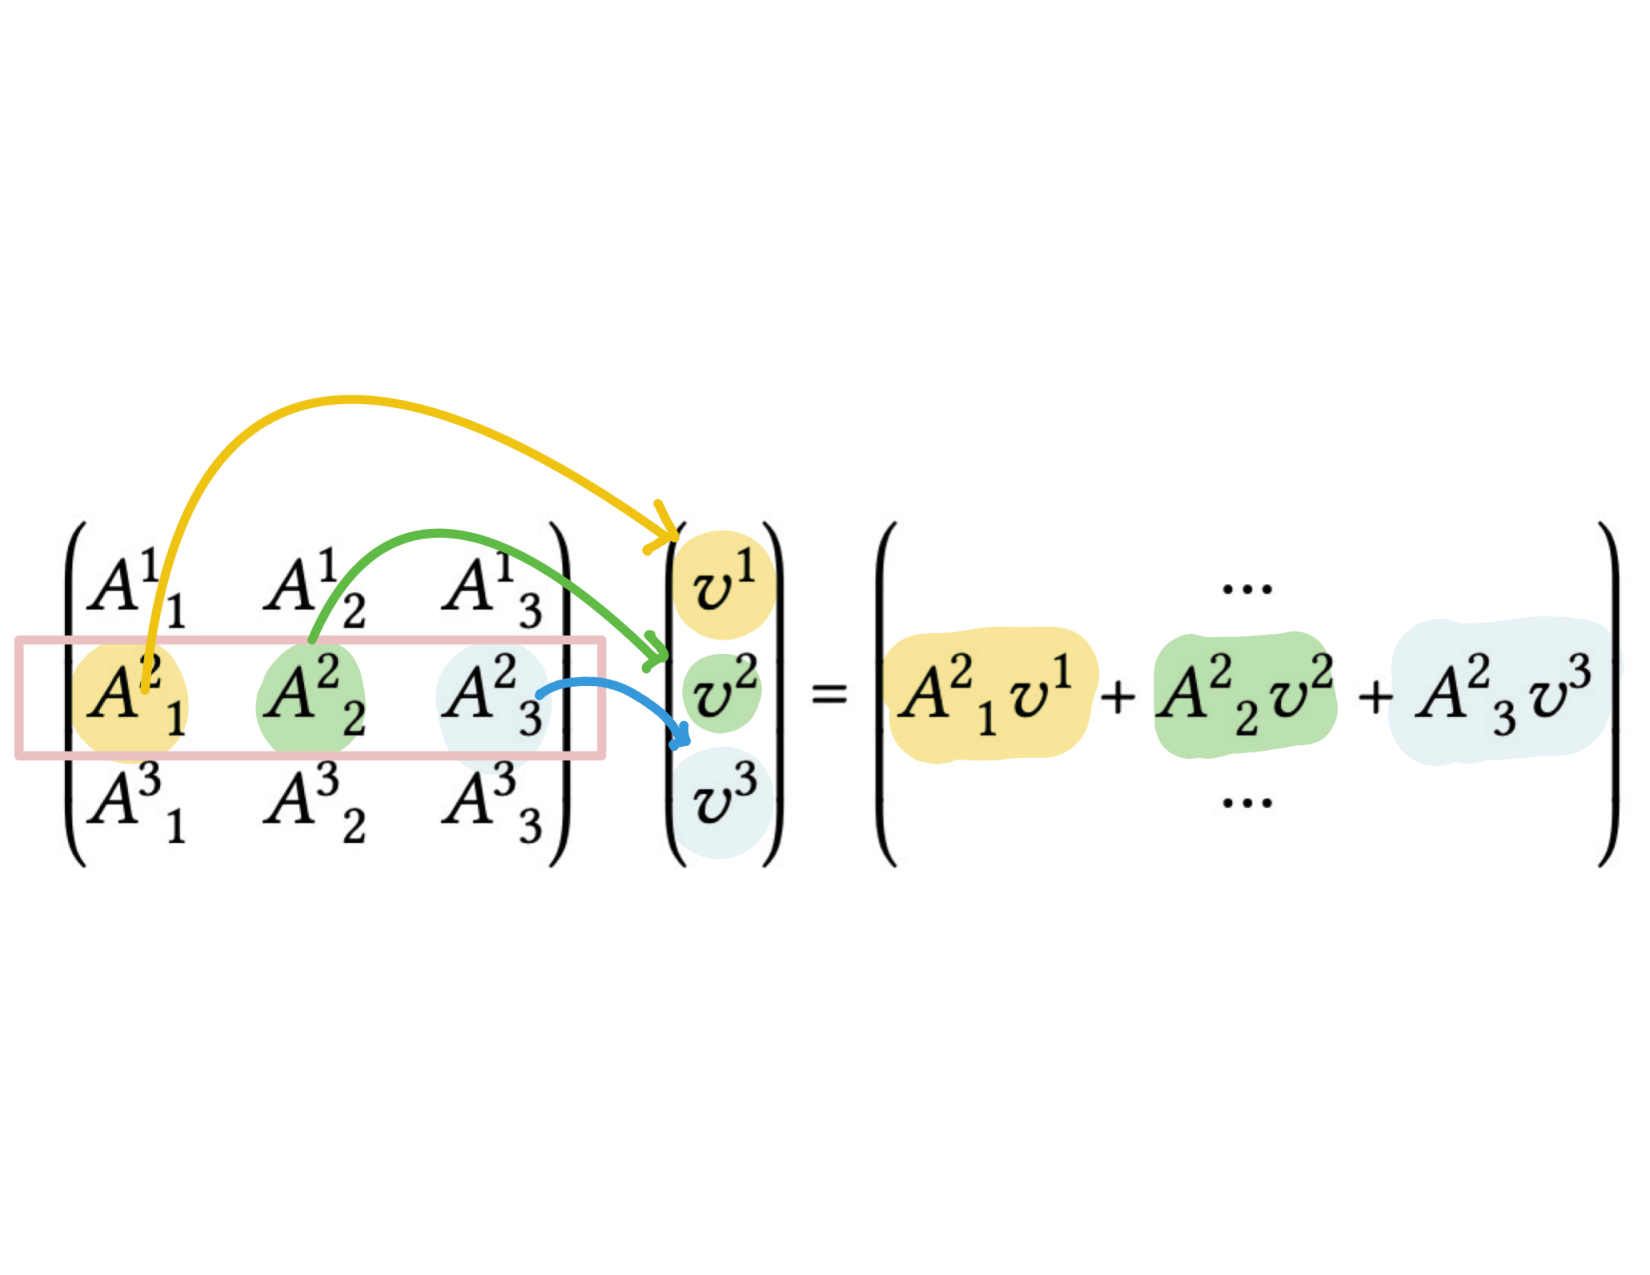
\includegraphics[width=.6\textwidth]{figures/matrixmultiplication.pdf}}
    }
\end{align}
The mechanical picture for this rule is best shown in real time. A rough summary is as follows. If matrix $A$ acts on vector $\vec{v}$, the value of the $i^\text{th}$ component of $A\vec{v}$ is calculated by:
\begin{enumerate}
  \item Take the $i^\text{th}$ \emph{row} of $A$.
  \item Rotate it clockwise by one quarter of a turn. Now it is aligned with the vector $\vec{v}$. Mentally place them right next to each other.
  \item Multiply the components that are horizontally next to each other.
  \item Sum together each product. This is $(A\vec{v})^i$.
\end{enumerate}
\begin{exercise}
Write this procedure in index notation. {Answer}: $(A\vec{v})^i = A\aij{i}{j}v^j$. Please take time to make sure that this is obvious. If it is not: work out the implied sum explicitly. You can even use the explicit case above, where $i=2$ and the indices run from $i,j \in \{1,2,3\}$. 
\end{exercise}

What is critical to emphasize at this stage is not yet the mechanical definition of the matrix multiplication procedure, but the following facts:
\begin{enumerate}
  \item When a matrix acts on a vector, the result is a vector. This is in contrast to a number or a covector or anything else. 
  \item When a matrix acts on twice a vector, the result is twice the previous result. That is: $A(2\vec{v}) = 2A\vec{v}$. The same is true for any rescaling by a number.
  \item When a matrix acts on the sum of two vectors, the result is the sum of the matrix acting on each vector independently: $A(\vec{v}+\vec{w}) = A\vec{v}+A\vec{w}$.
\end{enumerate}
What this tells us is that the object that we were calling a `matrix' colloquially---and that we may have been [erroneously] equating with a \acro{2D} array of numbers---is really a linear map from $V\to V$. Since this linear map takes objects (vectors) in $V$ and turns them into other objects in $V$, we call this a \textbf{linear transformation}\index{linear transformation}. 
%
So from now on we will be deliberate and talk about linear transformations from $V$ to $V$.

A quick remark: perhaps in ``Algebra II'' you worked with non-square matrices. A $n\times m$ matrix is a linear transformation that maps an $m$-dimensional vector into an $n$-dimensional vector. Clearly these are different vector spaces. In this course we are not interested in non-square matrices---there is an \emph{reason} we want to stick to the same vector space. And anyway, they will be infinite dimensional.
\begin{exercise}\label{ex:linear:transformation:are:matrices}
The ``Algebra II'' notion of a matrix is a square array of numbers that turns vectors into other vectors. From the definition of this multiplication, it should be clear that the transformation is linear. Show that \emph{any} linear transformation on a vector $\vec{v}$ can be represented as matrix multiplication. As a hint, you can start with the case of a one-dimensional vector where $\vec{v}$ is just a number. Remember that our definition of linear is slightly different from the $y=mx+b$ notion in basic algebra.
\end{exercise}
The above exercise makes it clear that the Algebra II idea of a matrix is exactly the same as a linear transformation from $V\to V$. The latter phase is one that we can generalize to tensors.

Let us add mathematical structure to our picture. Earlier we met the tensor product of two covectors, $\bra{i}\otimes\bra{j}$. This is an object that linearly `eats' a vector using $\bra{j}$ and then spits out a covector with basis $\bra{i}$. Another way of thinking about this is that the $\bra{j}$ acts on the vector and spits out a number. That number contributes to the coefficient of $\bra{i}$. This tensor structure is a map from $V\to V^*$. What does the tensor structure of a linear transformation $V\to V$ look like?

Following the same line of thought, it should be no surprise that a linear transformation from $V\to V$ can be expanded in terms of a basis of ``ket--bras'' $\ket{i}\otimes\bra{j}$. Because these linear transformations are so common, we typically drop the tensor product symbol and write
\begin{align}
  \ket{i}\otimes\bra{j} \to \ket{i}\bra{j} \ .
\end{align}
Thus the object that we used to call a `matrix' $A$ is expanded in components $A\aij{i}{j}$ as
\begin{align}
  A = A\aij{i}{j}\ket{i}\bra{j} \ .
\end{align}
Note the index structure carefully. The basis coefficient (or component) $A\aij{i}{j}$ has one upper index and one lower index. The upper index is first---it appears to the left---and indicates that the first object in the basis tensor product is a basis vector $\ket{i}$. The second index is lowered and indicates that the second object in the basis tensor is a basis covector, $\bra{j}$. 

The index structure of the coefficients now tells us everything there is to know about the basis. As a physicist, we may write\footnote{Or if we have self respect, we will only think this privately but never say it out loud lest any mathematicians hear us.} ``$A = A\aij{i}{j}$.'' By this we mean that we can \emph{fill in} the basis $\ket{i}\bra{j}$ just by looking at the indices. If we take this very glib shorthand, then we can imagine a linear transformation $A$ acting on a vector $\vec{v}$ by simply looking at their indices:
\begin{align}
 (Av)^i = A\aij{i}{j} v^j  \ .
\end{align}
We can tell ourselves the story that the ``lower index'' of $A\aij{i}{j}$ acts on the ``upper index'' of $v^j$ by contraction so that the $i^\text{th}$ component of $A\vec{v}$ is the sum $A\aij{i}{j} v^j$. Of course, what is actually going on is that the basis objects are doing all of the work ``under the hood'' of enforcing the linear transformation:
\begin{align}
  \left(A\aij{i}{j}\ket{i}\bra{j}\right) \left(v^k\ket{k}\right)
  &= A\aij{i}{j} v^k \ket{i} \langle j | k \rangle
  &= A\aij{i}{j} v^k \delta^j_k \ket{i}
  &= \left(A\aij{i}{j} v^j\right) \ket{i} \ .
\end{align}

\begin{exercise}
Okay, one last chance. If it is not completely obvious to you that $\left(A\aij{i}{j} v^j\right)$ is indeed the $i^\text{th}$ component of $A\vec{v}$, then work this out explicitly for the simple case of a $2\times 2$ matrix.
\end{exercise}

\begin{exercise}\label{ex:matrices:as:vectors}
Show that the space of linear transformations from $V\to V$ (the space of ``matrices'') is a vector space. The set of ket--bras (nobody really calls them that) $\ket{i}\bra{j}$ are a basis for this space. When $V=\mathbbm{R}^n$, we call the space $\text{GL}(N, \mathbbm{R})$, the \emph{general linear group}.
\end{exercise}

\begin{exercise}
Show that the a valid definition for a metric on the vector space $\text{GL}(N,\mathbbm{R})$ is 
\begin{align}
\langle A , B \rangle = \text{Tr}\left(A^\text{T} B\right) \equiv \left(A^\text{T}\right)\aij{i}{j}B\aij{j}{i} \ , 
\end{align}
the trace of $A^\text{T} B$ where $A^\text{T}$ is the transpose of $A$: $\left(A^\text{T}\right)\aij{i}{j} \equiv g_{ik}A\aij{k}{\ell}g^{\ell j}$. We motivate this definition below. 
\end{exercise} 



\begin{exercise}
Consider $\text{GL}(2,\mathbbm{R})$. A standard basis is $\ket{I}$ with $I\in\{1,2,3,4\}$ and defined with respect to the $\ket{i}\bra{j}$ as:
\begin{align}
  \ket{1} &= \ket{1}\bra{1}
  &
  \ket{2} &= \ket{1}\bra{2}
  &
  \ket{3} &= \ket{2}\bra{1}
  &
  \ket{4} &= \ket{2}\bra{2} \ .
\end{align}
Suppose $\ket{A}$ is an element of $\text{GL}(2,\mathbbm{R})$ with components $A^I$ in this standard basis. Now suppose we have a different basis written with respect to diagonal, symmetric, and antisymmetric matrices:
\begin{align}
  \ket{1'} &= \ket{1}\bra{1}
  &
  \ket{2'} &= \frac{1}{2}\left(\ket{1}\bra{2}+\ket{2}\bra{1}\right)
  \\
  \ket{3'} &= \frac{1}{2}\left(\ket{1}\bra{2}-\ket{2}\bra{1}\right)
  &
  \ket{4'} &= \ket{2}\bra{2} \ .
\end{align}
What are the components of $\ket{A}$ in the primed basis, $(A')^I$?
\end{exercise}

What else can we do with a linear transformation $A$ from $V\to V$? We already know that if we feed $A$ a vector, we get another vector. We could also `pre-load' $A$ with a covector in the same way that we `pre-loaded' the metric. Suppose $\tilde{\vec{w}}$ is such a covector. Then
\begin{align}
  \tilde{\vec{w}}A = 
  \left(\tilde{w}_i\bra{i}\right)
  \left(A\aij{j}{k}\ket{j}\bra{k}\right)
  =
  \tilde{w}_iA\aij{i}{k} \bra{k}
  \label{eq:row:acting:on:tensor}
\end{align}
is also a covector. This is obvious because it takes the form $(\text{coefficient})^i\bra{i}$ where the $\bra{i}$ are the basis covectors. 
% Note that we chose to write $\tilde{\vec{w}}=\tilde{w}_i\bra{i}$ to the left of $A$ because we knew that the covector basis vector $\bra{i}$ would act on the first argument of the $A$ basis tensor product, $\ket{j}$. However, once we have resolved the action $\langle i|j\rangle$, the coefficient $\tilde{w}_iA\aij{i}{k}$ of $\bra{k}$ is simply a number. Each of $\tilde{w}_i$ and $A\aij{i}{k}$ are simply \emph{numbers} that are multiplied. That means the order does not matter
%% This is a totally irrelevant aside.
This means that we can think of the linear transformations from $V\to V$ as, equivalently, linear transformations from $V^* \to V^*$. Alternatively, if we feed $A$ a covector and a vector, then we can form a \emph{bilinear} function from $V\times V^* \to \mathbbm{R}$ through
\begin{align}
  A(\tilde{\vec{w}}, \vec{v}) = \tilde{\vec{w}} A \vec{v} \ .
\end{align}
Here `bilinear' means that $A(\tilde{\vec{w}}, \vec{v})$ is linear in each of its two arguments. 

Thus we can interpret the linear transformation $A$ in three ways:
\begin{enumerate}
  \item A linear map from $V\to V$
  \item A linear map from $V^*\to V^*$
  \item A bilinear map from $V\times V^* \to \mathbbm{R}$.
\end{enumerate}
Each of these interpretations can be understood from the index structure of the components $A\aij{i}{j}$.
\begin{enumerate}
  \item We can contract the lower $j$ index with the upper index of a vector's components, $A\aij{i}{j}v^j$. After the contraction, there is only an upper index left so we know that the object is a vector. 
  \item We can contract the upper $i$ index with the lower index of a covector's components, $A\aij{i}{j}\tilde w_i= \tilde w_iA\aij{i}{j}$. After the contraction, there is only a lower index left so we know that the object is a covector. 
  \item We can contract each of the indices with the corresponding indices of a vector a covector. After the contraction, there are no indices left over and the object is simply a number.
\end{enumerate}

We see that the array of numbers (``matrix'') $A$ and its index structure tell us everything about the linear transformation, no matter \emph{which} linear transformation we are using. From now on, we shall refer to linear transformations by their coordinates, e.g.\ $A\aij{i}{j}$ rather than as a function $\vec{f}(\vec{v})$.






\subsection{Transformation = action on basis vectors}
The following should be a tautology\footnote{Or, as Tony Zee says: this is ``more obvious than obvious.''} if you know the action of a linear transformation on each of your basis vectors, then you know everything there is to know about the linear transformation. What we mean by this is that the components of a linear transformation simply tell you what that linear transformation does to your basis vectors. If a matrix $B$ has elments
\begin{align}
  B = 
  \begin{pmatrix}
    B\aij{1}{1} & B\aij{1}{2}\\
    B\aij{2}{1} & B\aij{2}{2}
  \end{pmatrix}
  = 
  B^{i}_{\phantom{i}j} |i\rangle\langle j| \ , 
\end{align}
then this means that acting with $B$ on basis vectors $\vec{e}_{(1)} = |1\rangle$ and $\vec{e}_{(2)} = |2\rangle$ gives
\begin{align}
  B|1\rangle &= B\aij{1}{1} |1 \rangle + B\aij{2}{1}|1\rangle 
  \\
  B|2\rangle &= B\aij{1}{2} |1 \rangle + B\aij{2}{2}|2\rangle  \ .
  \label{eq:B:basis:action}
\end{align}
In column vector notation:
\begin{align}
  B
  \begin{pmatrix}
  1 \\ 0
  \end{pmatrix}
  &= 
  \begin{pmatrix}
  B\aij{1}{1} \\ B\aij{2}{1}
  \end{pmatrix}
  &
  B
  \begin{pmatrix}
  0 \\ 1
  \end{pmatrix}
  &=
  \begin{pmatrix}
  B\aij{1}{2} \\ B\aij{2}{2}
  \end{pmatrix}\ .
\end{align}
So knowing the action on basis vectors is the same as knowing the transformation itself. 


\section{Inverse}

Given a linear operator $A$, the inverse operator $A^{-1}$ is defined by
\begin{align}
  A^{-1} A= A A^{-1} = \mathbbm{1}_{N\times N} \ .
  \label{eq:matrix:inverse}
\end{align}
What is the index structure of the $A^{-1}$ assuming that $A$ is a linear transformation from $V\to V$? We can remind ourselves by starting with $A^{-1}A\vec{v} = \vec{v}$. Then we recall that $A\vec{v}$ is some other vector in $V$. This means that $A^{-1}$ maps some vector, $A\vec{v}$, to another vector, $\vec{v}$. This means that $A^{-1}$ is also a map from $V\to V$. We expect the index structure to be the same: $A^{-1}$ is just another element in the space of linear transformations from $V\to V$. This means we can write the components of \eqref{eq:matrix:inverse} as
\begin{align}
  (A^{-1})\aij{1}{k} \, A\aij{k}{j} = \delta^i_j \ ,
  \label{eq:matrix:inverse:indices}
\end{align}
where we remind ourselves that the Kronecker $\delta$ can be written with the indices at the same horizontal position because $\delta\aij{i}{j} = \delta_j^{\phantom{j}i}$. 


For an $N$-dimensional vector space, \eqref{eq:matrix:inverse:indices} represents $N^2$ different equations: one for each combination of indices $i$ and $j$. These $N^2$ equations are, in principle, enough to determine the $N^2$ components $(A^{-1})\aij{i}{j}$ as a function of the components $A\aij{i}{j}$. Even though these are simply algebraic equations, they clearly become a huge pain in the ass to solve as $N$ becomes large. 



% The inverse operator, by the way, is also linear. 
% % Let's remind ourselves of what this means. 
% %
% Suppose I told you the action of the inverse transformation $A^{-1}$ on your basis vectors, vis-a-vis \eqref{eq:B:basis:action}:
% \begin{align}
%   A^{-1}|1\rangle &= x |1 \rangle + y|2\rangle 
%   \\
%   A^{-1}|2\rangle &= z |1 \rangle + w|2\rangle  \ .
%   \label{eq:Ainv:basis:action}
% \end{align}
% Then you know exactly how $A^{-1}$ acts on a general vector $|s\rangle = s^1|1\rangle + s^2 |2\rangle$:
% \begin{align}
%   A^{-1} |s\rangle &=
%   A^{-1} \left( s^1|1\rangle + s^2 |2\rangle \right)
%   \\ 
%   &=
%   s^1 A^{-1} |1\rangle + s^2 A^{-1} |2\rangle
%   \label{eq:Ainv:basis:action:on:gen:step2}
%   \\
%   &=
%   (s^1x + s^2z)|1\rangle + (s^1y + s^2 w)|2\rangle \ .
%   \label{eq:Ainv:basis:action:on:gen}
% \end{align}
% You can now keep this in mind when we say we want to solve $A|\psi\rangle = |s\rangle$. If we knew the action of $A^{-1}$ on some basis of the space, then the problem is simple:
% \begin{align}
%   |\psi\rangle = \psi^i |i\rangle 
%   &= \left( A^{-1} \right)^i_{\phantom{i}j} |i\rangle\langle j|
%   \, s^k|k\rangle 
%   \\
%   &= \left(A^{-1}\right)^i_{\phantom{i}j} s^k \, |i\rangle\langle j|
%   |k\rangle 
%   \\
%   &=\left(A^{-1}\right)^i_{\phantom{i}j} s^j \, |i\rangle \ .
% \end{align}
% We can write this as an equation for each component:
% \begin{align}
%   \psi^i &= \sum_j \left(A^{-1}\right)^i_{\phantom{i}j} s^j
%   \label{eq:Ainv:acting:on:source} \ .
% \end{align}
% We've restored the explicit sum over $j$ as a convenient reminder. The quantity $\left(A^{-1}\right)^i_{\phantom{i}j}$ is what we would like to identify with a Green's function; see Section~\ref{sec:lin:alg:greens} for a hint of that. From what we've learned in this subsection: knowing the components $\left(A^{-1}\right)^i_{\phantom{i}j}$ is exactly the same as \emph{knowing the action of the inverse operator on basis vectors}. 








\section{Adjoint}

Recall the definition of the transpose/Hermitian conjugate in \eqref{eq:transpose:as:inner:product:preloaded}. The `dagger' operation $\dag$ converts a vector into a covector using the inner product. For real vector spaces this is simply the transpose, for complex vector spaces it is the transpose and complex conjugation. We now define an operation on linear transformations $A$ that borrows the same notation: the \textbf{adjoint}\index{adjoint}. The adjoint of a linear transformation $A$ is denoted $A^\dag$ and is defined by the inner product relation:
\begin{align}
  \langle A^\dag \vec{w}, \vec{v} \rangle = \langle \vec{w}, A\vec{v}\rangle \ .
  \label{eq:def:adjoint}
\end{align}
This should look familiar from the bra-ket notation in quantum mechanics where we have $\langle w|A v\rangle = \langle A^\dag w|v\rangle$. The bra $\bra{w}$ is the Hermitian conjugate (dual) of some ket $\bra{w} = \ket{w}^\dag$, which is in turn defined with respect to the inner product. Following these definitions, one sees that this is equivalent to the adjoint definition \eqref{eq:def:adjoint}. This justifies the `overloading' of the $\dag$ operator: if $\vec{u} = A\vec{w}$, then
\begin{align}
  \bra{u} = \left(A \ket{w}\right)^\dag = \left(\ket{w}\right)^\dag A^\dag = \bra{w} A^\dag \ .
\end{align}
When $A$ is a matrix, then we can think about $\dag$ as literally meaning ``transpose and complex conjugate.'' When $V$ is a real vector space---so that linear transformations from $V\to V$ are also real---then $\dag$ is equivalent to transpose. 
\begin{example}
Show that 
\begin{align}
  \left(AB\right)^\dag = B^\dag A^\dag \ .
\end{align}
With foresight about naming variables, start with
\begin{align}
  \langle B^\dag \vec{w}, \vec{v}\rangle = \langle \vec{w}, B \vec{v} \rangle \ .
\end{align}
Now assume that $\vec{w} \equiv A^\dag \vec{u}$. Plugging this in and using the definition of the adjoint gives:
\begin{align}
  \langle B^\dag A^\dag \vec{u}, \vec{v}\rangle 
  = \langle A^\dag \vec{u}, B \vec{v} \rangle 
  = \langle \vec{u},  (AB) \vec{v} \rangle 
  = \langle (AB)^\dag \vec{u},   \vec{v} \rangle 
  \ .
\end{align}
This proves the proposed relation. You should recognize this from the real case where $(AB)^\text{T} = B^\text{T}A^\text{T}$ \ .
\end{example}

What does the adjoint of a matrix look like in terms of indices? In fact, one could ask the following question. What is the index structure of $A^\dag$? We could even restrict for simplicity to real spaces so that we really want to know: what are the positions of the indices of $A^\text{T}$? We know that $A^\text{T}$ is still a linear map from $V\to V$. This means it has one upper and one lower index. We can then ask how these indices are oriented: 
\begin{align}
  A\aij{i}{j} &= \left(A^\text{T}\right)\aij{j}{i}
  &
  \text{or}
  &
  &
  A\aij{i}{j} &= \left(A^\text{T}\right)_j^{\phantom{j}i} \ .
\end{align}
Which one is it? The fact that we write $A^\text{T}\vec{w}$ in the defining relation for the adjoint means that $A^\text{T}$ is a linear transformation from $V\to V$, which tells us that it is the same class of object as $A$ and should thus have the same index structure. Write this index structure out explicitly in the definition of the adjoint, \eqref{eq:def:adjoint}, written with the inner product notation replaced by the metric:
\begin{align}
  \left(A^\text{T}\right)\aij{i}{k}w^k v^j g_{ij}
  &= 
  w^i A\aij{j}{k}v^k g_{ij} \ .
\end{align}
We are about to do something slick, but first we re-label the indices for future convenience. Relabeling dummy indices does not change anything.
\begin{align}
  \left(A^\text{T}\right)\aij{i}{k}w^k v^j g_{ij}
  &= 
  w^k A\aij{i}{j}v^j g_{ki} \ .
  \label{eq:transpose:components:1}
\end{align}
On the right-hand side we chose indices so that we have $A\aij{i}{j}$ as a factor. Conveniently, on left-hand side the dummy indices of the $w$ and $v$ coefficients match. Because the above equality is true for \emph{any} kets $\vec{v}$ and $\vec{w}$, then we can simply cancel $w^kv^j$ on both sides:
\begin{align}
  \left(A^\text{T}\right)\aij{i}{k} g_{ij}
  &= 
  A\aij{i}{j} g_{ki} \ .
  \label{eq:transpose:components:2}
\end{align}
\begin{exercise}
Explain why step from \eqref{eq:transpose:components:1} to \eqref{eq:transpose:components:2} is valid.
\end{exercise}
  Now we may contract both sides with $g^{j\ell}$. Using the fact that this is the inverse metric so that $g^{j\ell}g_{ij} = \delta^\ell_i$, we have
\begin{align}
  \left(A^\text{T}\right)\aij{\ell}{k}
  = 
  g_{ki}
  A\aij{i}{j} 
  g^{j\ell}
. 
\end{align}
This gives an index definition of $A^\text{T}$. 
\begin{exercise}
Using similar manipulations, show that
\begin{align}
  A\aij{
  i}{j} = g_{j\ell} \left(A^\text{T}\right)\aij{\ell}{k} g^{ki} 
  = \left(A^\text{T}\right)_i^{\phantom{i}j} 
  \ .
\end{align}
We see that we end up with an unusual index structure on the right-hand side. At first glance we may be worried that this is not the index structure of a linear transformation from $V\to V$ like we are used to. However, we also now have the rule that indices are raised and lowered uniquely by the metric. Thus the expression $\left(A^\text{T}\right)_i^{\phantom{i}j}$ is completely determined from $\left(A^\text{T}\right)\aij{i}{j}$ through the implicit action of the metric.
\end{exercise}


\begin{exercise}
Show that $\left(A^\dag\right)^\dag = A$ \ .
\end{exercise}



You may recall from linear algebra that there was something \emph{nice} about symmetric matrices. It is the same thing that is \emph{nice} about Hermitian operators in quantum mechanics. Both are \textbf{self-adjoint}\index{self-adjoint}, meaning $A^\dag = A$. Self-adjoint operators are nice because they have real eigenvalues, even if the vector spaces they act on are not necessarily real.\footnote{You may care about this if $A$ is supposed to correspond to a physical observable.}


\section{Multilinear Transformations} % Tensors

Linear algebra should feel very familiar because most of us have played with matrices in various forms throughout our mathematical education. If you are like me, then at some point in your education you hear the word `\textbf{tensor}' and you feel like it is some exotic new class of object with a slew of unknown mathematical structure. This is not the case. We now make a point to understand what a tensor is and to realize that it is simply an extension of linear maps between vector spaces. 

From the previous section we know that given a vector space $V$, perhaps $\mathbbm{R}^n$, we can consider the space of linear transformations from $V\to V$.\footnote{If you did Exercise~\ref{ex:matrices:as:vectors}, then you know that these transformations are themselves a vector space. Then you could consider  linear transformations on the space of linear transformations...} This space formalizes what we called \emph{matrices}. It gave us three maps: $V\to V$, $V^* \to V^*$, and $V\times V^*\to \mathbbm{R}$. In the latter case, we called the transformation \emph{bilinear} because it is linear in each argument. 

The generalization that we now make is a linear transformation of the form:\footnote{And eventually we also include complex functions, where we replace $\mathbbm{R}\to \mathbbm{C}$. }
\begin{align}
  V\times \cdots \times V \times V^* \times\cdots\times V^* \to \mathbbm{R}
\end{align}
That is: a linear map that takes some number of vectors and some number of covectors and returns a number. Because the map is linear in each argument, we say that they are \emph{multilinear}. Maybe the reason why this is `scary' the first time we see it is that the components of tensors, in general, have many indices.\footnote{There are various phobias about insects with many legs. Perhaps for similar reasons.} From our experience with ``matrices,'' we know that the multilinear map above can be interpreted in many ways. The same object may, for example, map some number of vectors and covectors into some other number of vectors and covectors.



\begin{example} \label{eg:multilinear:2vec:to:1vec}
Consider a multilinear map that takes two vectors and spits out a third vector. This is a tensor. As stated, we can think of this as a function $\vec{f}(\vec{v},\vec{w})$ where we understand that $\vec{f}$ itself is a vector.\footnote{As I squint at my screen I realize that it may not be clear that $\vec{f}$ is boldfaced. You can mentally put a $\overrightarrow{\vec{f}}$ everywhere.} We are assuming that we all agree on some basis and there's no need to explicitly write $\vec{v}=v^i\hat{\vec{e}}_{(i)}$. Multilinearity means
\begin{align}
  \vec{f}(\alpha\vec{v}+\beta\vec{u},\vec{w}) &= 
  \alpha\vec{f}(\vec{v},\vec{w}) +
  \beta \vec{f}(\vec{u},\vec{w})
  \\
  \vec{f}(\vec{v},\alpha\vec{w}+\beta\vec{x}) &= 
  \alpha\vec{f}(\vec{v},\vec{w}) +
  \beta \vec{f}(\vec{v},\vec{x}) \ ,
\end{align}
where $\alpha$ and $\beta$ are numbers. The function $\vec{f}$ is simply linear in each of its two arguments: it is \emph{multi}linear. (There's really nothing deep here, eh?) Then we recognize that $\vec{f}$ itself has an index. So the above multilinearity conditions may be written in component form:
\begin{align}
  f^i(\alpha\vec{v}+\beta\vec{u},\vec{w}) &= 
  \alpha\vec{f}(\vec{v},\vec{w}) +
  \beta \vec{f}(\vec{u},\vec{w})
  \\
  f^i(\vec{v},\alpha\vec{w}+\beta\vec{x}) &= 
  \alpha\vec{f}(\vec{v},\vec{w}) +
  \beta \vec{f}(\vec{v},\vec{x}) \ ,
\end{align}
where the relations are separately true for each index $i$. 
\end{example}

Because you did Exercise~\eqref{ex:linear:transformation:are:matrices}---\emph{you did do this exercise, right?}---you now should intuit that you can represent the information in a multilinear transformation as some array of numbers. This is the same as saying that you can represent a linear transformation as a $N\times N$ array that we call a matrix.\footnote{Even though I keep saying we need to stop calling it that.} 

\begin{exercise}
Consider the multilinear map $\vec{f}$ in Example~\ref{eg:multilinear:2vec:to:1vec}. Suppose the vector space is 2-dimensional, for simplicity. Write out the $2^3$ components of the tensor corresponding to $\vec{f}$. As extra credit\footnote{Whenever I mention `extra credit' please know that I am imagining the skit ``That's Numberwang!'' from the British comedy show \emph{That Mitchell And Webb Look}.}, convince yourself that you can write this as a $2\times 2\times 2$ cube of numbers. 
\end{exercise}

\begin{exercise}
Convince yourself\footnote{This is my way of saying: you do not have to do a full mathematical proof, but think about this until it is absolutely clear that it is true.} that the function $\vec{f}$ in Example~\ref{eg:multilinear:2vec:to:1vec} is \emph{equivalently} all of the following:
\begin{itemize}
  \item A linear map from $V\times V \to V$ .
  \item A linear map from $V \to  V^*\times V$. Note that the output of this map is a linear transformation from $V\to V$. 
  \item A linear map from $V^*\to V^* \times V^*$ .
  \item A linear map from $V^*\times V \to V^*$ .
  \item A linear map from $V \times V \times V^* \to \mathbbm{R}$ \ .
\end{itemize}
Are there other linear maps one can construct from this? 
\end{exercise}
Tensors are precisely these multilinear maps. This is in exactly the same that vectors and covectors are linear maps on each other. It is also in exactly the same way that linear transformations from $V\to V$ are also linear transformations from $V^*\to V^*$ and bilinear maps from $V\times V^* \to \mathbbm{R}$. We could read all of this off of the index structure of the linear transformation. In the same way, the index structure of the multilinear transformations tell us all of these things.



\section{Tensor Indices}
\label{sec:indices:II}

% In Section~\ref{sec:indices:I} we presented the metric/inverse metric as some kind of re-writing of the ``transpose'' operation. We very deliberately explained this as raising or lowering an index. At the time it may have seemed like an overkill of mathematical structure.

% NOW: we're generalizing the types of things we can imagine acting on. Linear transformations, for exampl.e 

Multilinear maps (tensors) are linear combinations of a tensor product of basis vectors and covectors. For every vector argument that a multilinear map takes in, there is a basis covector (a basis linear map from $V\to \mathbbm{R}$). For every covector argument that a multilinear map takes in, there is a basis vector (a basis linear map from $V^*\to \mathbbm{R}$). Alternatively, you do not have to think of the basis covector as taking in a vector as an argument, but rather outputting a covector as an output. All of this is clear from the index notation: a lower index can either contract with an upper index (eating a vector) or it can be a leftover index after other contracts (pooping a covector). 

When you act with a tensor product on some object, one must specify how the bras and kets in the product are supposed to `hit' the object. For example, consider the following tensor product:
\begin{align}
\tens{T} \equiv
  T^{ijk}_{\phantom{ijk}\ell m n}\ket{i}\otimes\ket{j}\otimes\ket{k}
  \otimes\bra{\ell}\otimes\bra{m}\otimes\bra{n} \ .
\end{align}
I can act with $\tens{T}$ on a vector $\vec{v} = v^i\ket{i}$. To do this, one of the basis bras in $\tens{T}$ needs to act on the ket in $\vec{v}$. We need to specify which one.\footnote{In practice we rarely actually have to to this. This is because we usually symmetrize and antisymmetrize the upper and lower indices so that it does not matter which index is acting on the object. In my life I am fortunate to rarely have to work with objects with large numbers of indices with mixed symmetrizations and antisymmetrizations. Then there are the folks who work on tensor networks...} I could tell you in words that $\tens{T}$ acts on $\vec{v}$ through its fourth argument---the one corresponding to the $\bra{k}$ basis bra. That is cumbersome, but gives the following:
\begin{align}
  \tens{T}\vec{v} &= T^{ijk}_{\phantom{ijk}\ell m n}
  v^p
  \ket{i}\otimes\ket{j}\otimes\ket{k}
  \otimes\bra{\ell}\otimes\langle m|p\rangle\otimes\bra{n}
  \\ &=
  T^{ijk}_{\phantom{ijk}\ell m n}
  v^m
  \ket{i}\otimes\ket{j}\otimes\ket{k}
  \otimes\bra{\ell}\otimes\bra{n} \ .
\end{align}
We have used $\langle m|p\rangle = \delta^m_p$. Now we notice one of the benefits of ``lazy physicist'' index notation: suppose we just looked at the \emph{components} of $\tens{T}\vec{v}$. These are the coefficients $T^{ijk}_{\phantom{ijk}\ell m n}v^m$. Simply by looking at these components, we know that
\begin{enumerate}
  \item The object $\tens{T}\vec{v}$ has three vector indices and two dual vector indices. The upper index is contracted with a lower index is not a `free' index, it is a `dummy' index that has been summed over. 
  \item We know that the basis vectors must be $\ket{i}\otimes\ket{j}\otimes\ket{k}
  \otimes\bra{\ell}\otimes\bra{n}$ simply because they must contract the indices of the components.
  \item We know \emph{which} index in $\tens{T}$ contracts with the index in $\vec{v}$ because that is the dummy index contraction. We can see from $T^{ijk}_{\phantom{ijk}\ell m n}v^m$ that the fifth index of $\tens{T}$ contracts with the upper index of $\vec{v}=v^m |m\rangle$.
\end{enumerate}
In Section~\ref{sec:indices:symmetries} we present one more powerful feature of index notation: our ability to read off how a given tensor changes when we either (a) transform our coordinates or (b) transform the physical object that the tensor describes.

\begin{exercise}
This is the tensor version of Exercise~\ref{ex:linear:transformation:are:matrices}. Convince yourself that any multilinear map that takes arguments from a vector space $V$ and its dual $V^*$ may be represented as a tensor. It helps to reduce this problem to multiple instances of linear maps as in Exercise~\ref{ex:linear:transformation:are:matrices}.
\end{exercise}

\begin{example}
Is $T^{ijk}_{\phantom{ijk}\ell m n}v^m = v^m T^{ijk}_{\phantom{ijk}\ell m n}$? The answer is yes. There may be a part of you that instinctively reacts poorly to this because you are used to matrices not commuting: in general, $AB \neq BA$ for matrices $A$ and $B$.\footnote{In fact, if $A$ is an $n\times m$ matrix and $B$ is an $m\times n$ matrix with $n\neq m$, $AB$ is an $n\times n$ matrix and $BA$ does not even mathematically make sense. Though I did promise that all of our matrices would be square in this course. In the jargon of beatniks, that would mean that our matrices are ``boring,'' but in our class that means that they are ``nice.''} Surely tensors do not commute in general. We are in luck: neither $T^{ijk}_{\phantom{ijk}\ell m n}$ nor $v^m$ are formally tensors. They are \emph{components} of tensors: they are simply numbers, and so they commute. For example, the action of a covector on a vectors is
\begin{align}
\tilde{\vec{w}}\vec{v}  = w_iv^i
= w_1v^1 + w_2v^2 + \cdots = v^1 w_1 + v^2w_2 + \cdots = v^i w_i \ .
\end{align}
Each term is a product of numbers. When we defined a vector space we needed some abstract mathematical structure (the ``vectorness'' carried by a basis vector), and a definition of numbers that we can use to define linear combinations of vectors. The class numbers are formally called \emph{fields}.\footnote{I have no idea what the formal definition of a field is. I am on a plane as I write this and frankly I do not care enough to pay \$8 for in-flight wifi to look it up.} One of the properties of a field is that the multiplication of two elements is commutative. This is one of the reasons why that is a nice property to have.
\end{example}


% \begin{example}
% Transformation of fields. Mixture of active and passive.
% \end{example}


\section{Indices and Symmetries}
\label{sec:indices:symmetries}

Earlier we made the point that writing objects in terms of indices makes quite a lot of sense when those objects are linear maps between vector spaces. There is a second reasons why physicists love indices: they are a natural language for capitalizing on the symmetries of a system.\footnote{The mathematical study of symmetries is called group theory. Sometimes people distinguish this from representation theory, which is loosely the study of how objects transform with respect to symmetries---in contrast to the underlying structure of a class of symmetries. This lies outside the scope of our course, but you are likely to have had some training in representation theory when you invoked Clebsch--Gordan coefficients in quantum mechanics.}


\section{Eigenvalues and Eigenvectors}

\label{sec:eigenvectors}

Given a sufficiently \emph{nice} linear transformation, $A\aij{i}{j}$, there is a particularly convenient basis: the \textbf{eigenvectors} of $A$. These are vectors $|\lambda\rangle$ such that
\begin{align}
  A |\lambda\rangle = \lambda |\lambda\rangle \ .
\end{align}
In other words, $A$ acts on the eigenvector by rescaling. The rescaling coefficient is the eigenvalues. For \emph{nice} transformations (see Section~\ref{sec:niceness}), there is a complete set of such vectors to span the vector space. 
\begin{exercise}
If you are particularly keen, figure out (or look up) the mathematical conditions for a transformation $A$ to have a set of eigenvectors that form a basis of the vector space. As an added bonus, check that these eigenvectors are orthogonal.
\end{exercise}

If you write a general vector $|v\rangle$ in terms of this eigenbasis,
\begin{align}
  |v\rangle = v^i |\lambda_{(i)} \rangle \ ,
\end{align}
Then the action of $A$ on this vector is easy:
\begin{align}
  A |v\rangle = \sum_i \lambda_{(i)} v^i |\lambda_{(i)} \rangle \ .
\end{align}
In fact, assuming that all of the eigenvalues are non-zero, even the matrix inverse is easy:
\begin{align}
  A^{-1}|v\rangle = \sum_i \lambda_{(i)}^{-1} v^i |\lambda_{(i)} \rangle \ .
  \label{eq:linear:aglebra:inverse:eigenvectors}
\end{align}
Hey, that is kind of a big deal. Taking the inverse of a matrix is a much harder problem than acting with the matrix on a vector.\footnote{This is a general truth that ``inverse problems'' are very difficult. This is well known in applied mathematics, but the era of `big science' has made it clear that many of the frontiers in physics and astronomy are inverse problems.}
The first time you see this should have brought a deep joy to your life: if you can decompose a matrix (linear transformation) into its eigenvectors and eigenvalues, then taking the inverse transformation is simple.





\section{What about traces and determinants?}

There are two matrix operations that we have known about since childhood: the trace and the determinant. The children's-version of these two quantities for a matrix $M$ are:
\begin{itemize}
  \item The trace is the sum of the diagonal components: $\text{Tr}\,M \equiv M\aij{1}{1} + M\aij{2}{2}+\cdots_{}$.
  \item The determinant is some obscure sum of products of the components of $M$ with some delicate choice of minus signs. The determinant of $N\times N$ matrices is recursively related to the determinant of $(N-1)\times (N-1)$ matrices.\footnote{Cramer's rule.}
\end{itemize}
Now that we are sophisticated adults, we may wonder: why should we ever care about these two operations? After all, we now appreciate that the components of a matrix are basis-dependent quantities whereas the linear operators encoded by matrices are basis independent. This is like asking if the first component of a vector has any intrinsic significance---it does not, because in a different basis the same vector has a different first component.

The reason why the trace and the determinant of a matrix are significant are that they are actually basis independent numbers associated with each matrix. To see this, let us write out the trace and determinant more carefully. 

The \textbf{trace}\index{trace} of a matrix $M$ is
\begin{align}
\text{Tr}\,M \equiv  
  M\aij{i}{i} 
  = \delta^{j}_{i}M\aij{i}{j} 
  = M\aij{1}{1} + M\aij{2}{2}+\cdots \ .
\end{align}
Observe that the trace carries no free indices but is built out of covariant quantities. Therefore the trace is invariant. The trace does not require the metric.

\begin{exercise}
Check explicitly that the trace of a $2\times 2$ matrix in two-dimensional Euclidean space is invariant under rotations. Write out a matrix $M$ and perform the rotation $M\to M' = RM R^T$. Show that the sum of diagonal elements of $M'$ is equivalent to the sum of diagonal elements of $M$. All you need is $\sin^2\theta + \cos^2\theta = 1$.
\end{exercise}

\begin{example}
Individual quantum states---say a spin-1/2 state, or qubit---are vector spaces. When two quantum states are \emph{entangled}, then the observation of one of the states will project the other state. In this case, the system is a statistical ensemble rather than a quantum state. We call these \textbf{mixed states}. This is in contrast to \textbf{pure states}, which are vectors in a Hilbert space. Mixed states are described by a \textbf{density matrix},
\begin{align}
  \rho = \sum_i p_i|i\rangle\langle i| \ ,
\end{align}
where $p_i$ is the \emph{probability} (not the amplitude) for state $|i\rangle$. Mixed states are defined by $\text{Tr}\,\rho^2 <1$, while pure states satisfy $\text{Tr}\,\rho^2 =1$.
\end{example}

The \textbf{determinant} of a matrix is a bit trickier. A useful definition for an $N$-dimensional vector space is
\begin{align}
  \text{det}\,M \equiv 
  \epsilon_{i_1i_2\cdots i_N} 
    M\aij{i_1}{1} M\aij{i_2}{2}\cdots M\aij{i_N}{N} . 
    \label{eq:det:def}
\end{align}
Here $\epsilon_{i_1i_2\cdots i_N}$ is the $N$-dimensional \textbf{Levi-Civita symbol}.\footnote{Tullio Levi-Civita was an Italian mathematician with a compound last name, not two separate people. Typographically, one writes `Levi-Civita' with a dash, while one writes the concatenation of two different people's last names with an en-dash, e.g.\ `Randall--Sundrum models.'}
%
It is defined to be totally antisymmetric in each of its components:
\begin{align}
  \epsilon_{i_1i_2\cdots i_{k}i_{k+1}\cdots i_N} 
  =
  -
  \epsilon_{i_1i_2\cdots i_{k+1}i_{k}\cdots i_N}  \ .
\end{align}
This leaves an overall sign to be chosen by convention, which we usually take to be $\epsilon_{123\cdots N} = 1$. It should be clear that the Levi-Civita symbol is zero when any of its indices are repeated: $\epsilon_{11\cdots} = 0$. 
\begin{exercise}
Confirm for the $2\times 2$ case that the definition \eqref{eq:det:def} corresponds to the usual definition of the $2\times 2$ determinant:
\begin{align}
  \det
  \begin{pmatrix}
    a & b \\ c& d
  \end{pmatrix}
  \equiv ad - bc \ .
\end{align}
\end{exercise}
The Levi-Civita symbol is not formally a tensor. In $N$-dimensional space it has $N$ indices, but it does not transform. For spaces with no curvature this distinction is a formality, though one must be a bit more careful in curved space(time).\footnote{See the opening chapter of Carroll's \emph{Spacetime and Geometry}.}

You may object that \eqref{eq:det:def} does not look invariant: there are explicit matrix components written out. We can write it in a more manifestly invariant form by employing another Levi-Civita symbol:
\begin{align}
  \text{det}\,M \equiv 
  \frac{1}{N!}
  \epsilon_{i_1i_2\cdots i_N} 
  \epsilon^{j_1j_2\cdots j_N} 
    M\aij{i_1}{j_1} M\aij{i_2}{j_2}\cdots M\aij{i_N}{j_N} ,
    \label{eq:det:def:invariant}
\end{align}
where the upper-index Levi-Civita symbol is defined the similarly. You can treat it as taking the Levi-Civita symbol with lower indices and raising the indices using the inverse metric.\footnote{This gets a little subtle and is outside our scope. It intersects with a few important ideas in differential geometry: the signature of the metric, and the idea of a tensor density. See, e.g.~\url{https://physics.stackexchange.com/a/292606}} The factor of $1/N!$ accounts for a combinatoric multiplicity.
\begin{exercise}
Derive the $1/N!$ factor in \eqref{eq:det:def:invariant} by requiring that the expression matches \eqref{eq:det:def}.
\end{exercise}

The determinant encodes the volume of the space. This is most easily seen by looking at low-dimensional examples. 
\begin{exercise}
Let $A$ be the $2\times 2$ matrix whose columns are two vectors, $\vec{v}$ and $\vec{w}$. Show that $\det A$ is the area of the parallelogram formed by $\vec{v}$ and $\vec{w}$. Do the same for a three dimensional matrix; the determinant is the volume of the parallelpiped whose edges are the vectors given by the columns of the matrix.
\end{exercise}
This is why multidimensional integrals in curvilinear coordinates carry a determinant of the Jacobian: it encodes the fact that the little hyper-cubes that we use in curvilinear coordinates do not all have the same volume. 
\begin{example}
The integration measure in $\mathbbm{R}^2$ takes different forms in polar versus Cartesian coordinates. In Cartesian coordinates we have $dx\,dy$. In polar coordinates the integration measure is
\begin{align}
  dx\,dy = \left|\frac{\partial \vec{x}}{\partial \vec{r}} \right| dr\,d\theta \ ,
\end{align}
where the determinant of the Jacobian is
\begin{align}
  \left|\frac{\partial \vec{x}}{\partial \vec{r}} \right|
  &= 
  \det
  \begin{pmatrix}
  \frac{\partial x}{\partial r}  
  &
  \frac{\partial y}{\partial r}  
  \\
  \frac{\partial x}{\partial \theta}  
  &
  \frac{\partial y}{\partial \theta}  
  \end{pmatrix}
  =
  (\cos\theta)(r\cos\theta) - (\sin\theta)(-r\sin\theta) = r \ .
\end{align}
We thus find that $dx\,dy = rdr\,d\theta$ \ .
\end{example}




\chapter{Vector fields on manifolds}
\label{chap:vector:fields}
% motivating transformation
% https://www.youtube.com/watch?v=2MC4xMhscjQ
% \flip{To Be Filled In}

\flip{this section badly needs pictures}

\section{Space(time) as a manifold}

Space (or spacetime if we are relativistic) is not a vector space. For example, space may have more symmetries than a vector space. Translations are one such example: you cannot translate a vector. A vector of unit length pointing in the $\hat{y}$ direction is fully specified: it makes no sense to talk about `` vector of unit length pointing in the $\hat{y}$ direction'' \emph{but translated so that its base is at $(x,y)=(1,0)$}. 

We say that space is a \textbf{manifold}\index{manifold}. This has a formal definition in differential geometry, but we stick to physical intuition here.\footnote{It is dangerous to venture off into the wilderness of science using only physical intuition. Let us not stray very deep into the woods.} Sometimes we also call it the \textbf{base space}\index{base space}. 

We typically care about functions on this manifold. These are maps $f: M\to$ numbers. For example, a topographic map is a map from the manifold of longitude and latitude coordinates to numbers. The number assigned to each point is the height above sea level. 
\textfig[1]{figures/manifold3a.pdf}{A function maps points on a manifold to numbers.}{fig:manifold:map}

\section{Tangent plane as a vector space}

There are vector spaces associated with a space(time). In fact, there are usually an infinite number of vector spaces for a spacetime. At each point $p\in M$, there is a plane that is tangent to $M$ that `touches' $p$. We call this the \textbf{tangent plane} of $M$ located at $p$, or $T_pM$\index{tangent plane}. This tangent plane is a vector space. A good way to think of the vectors in this space is to think of them as \emph{velocity vectors}.
\textfig[1]{figures/manifold1.pdf}{A manifold $M$ and the tangent plane at point $p \in M$.}{fig:manifold:1}
Each point has its own tangent plane. Here's another point $p'$ on $M$ with a different tangent plane $T_{p'}M \neq T_p M$:
\marginfig{figures/manifold2.pdf}{A manifold $M$ and the tangent plane at point $p' \in M$.}{fig:manifold:2}

Suppose you have a curve $\gamma$ in $M$. This is a map that takes a real number, $t$, and outputs $\gamma(t)$, a point in $M$. The dependence on the real number is called the parameterization of the curve. If we are hikers on the manifold, $\gamma(t)$ is our path through the mountains and valleys of the manifold. Suppose that at $t_0$ the curve is at some point $x_0\in M$: $\gamma(t_0) = p$. Then we can determine our velocity at time $t_0$ (and location $p$) by taking the time derivative: $\gamma'(t_0) = \left.d\gamma/dt\right|_{t_0}$. In general, $\gamma'(t_0)$ is a $d$-dimensional vector where $d$ is also the dimensionality of the manifold. 

$\gamma'(t_0)$ does \emph{not} live on the manifold. It lives on the tangent space, $T_{\gamma{t_0}}M$. Take a moment to appreciate this. It is obvious if you draw a picture; see Fig.~\ref{fig:manifold:3}.
\textfig[1]{figures/manifold3.pdf}{The change in a function $f$ along a path $\gamma(s)\in M$.}{fig:manifold:3}

In a spacetime, these tangent planes are geometrically what we mean by locally inertial frames. We can approximate the neighborhood around a single point of a curved spacetime with the tangent plane. The tangent plane is a `flat space' which looks like Minkowski space (special relativity). The deviation from the tangent plane as we move further away from that point is encoded by general relativity. In fact, you can see what goes wrong: if we want to talk about vectors at some other point, $p'$, then formally we are talking about a completely different vector space, $T_{p'}M \neq T_pM$. The mathematical machinery of differential geometry (or general relativity) is focused on making sense of how one transports vectors from one vector space to nearby vector spaces. This is called parallel transport\index{parallel transport}.

The fact that you have as many tangent planes as you have points in $M$ means that our entire construction is actually a collection of the base space and an infinite number of tangent spaces. We call this bundle of tangent spaces... well, that is exactly what we call it: a \textbf{tangent bundle}. The spaces of one-forms (covectors) associated with each vector space in the tangent bundle is called a cotangent bundle. You may want to put other stuff on your base space, for example something encoding the electromagnetic gauge choice at each position. Those are also bundles. In general, some space that is attached at each position of the base space is called a fiber. This whole construction is called a \textbf{fiber bundle}\index{fiber bundle}.

\section{Partial derivatives as vectors}

A basis that is not at all obvious---but turns out to be rather natural---for vectors in the tangent plane are the partial derivatives: $\partial_x = \partial/\partial x$, $\partial_y$, and so forth. 
\marginfig{figures/manifold4.pdf}{Partial derivatives as basis vectors for the tangent bundle.}{fig:manifold:4}
\begin{exercise}
Convince yourself that partial derivatives form a vector space. Start by reminding yourself of the definition and requirements of a vector space.
\end{exercise}
Why is this a sensible basis? Let $M$ be the space manifold. We typically care about functions that take points in $M$ and spit out numbers. Consider the topographic map example: it takes in longitude and latitude and outputs the height above sea level. 
Let $\gamma(t)$ be our path as we are jogging along some trail through the mountains. One thing we may want to know is the rate at which we are increasing our height as we jog. Suppose that at time $t$ we are at position $p = \gamma(t)$. The rate at which our altitude is increasing is 
\begin{align}
  \frac{\partial f}{\partial x}
  \frac{d\gamma_x(t)}{dt}
  +
  \frac{\partial f}{\partial y}
  \frac{d\gamma_y(t)}{dt} 
  =
  \dot\gamma(t)\cdot \nabla f
  \ ,
\end{align}
where $\gamma_x$ and $\gamma_y$ are the $x$- and $y$- components of $\gamma$. The coefficients ${d\gamma_{x,y}(t)}{dt}$ are your velocity components. We see that $\partial_{x,y}$ naturally forms a basis. It does not matter what $f$ is, we can plug in whatever $f: M\to \mathbbm{R}$ we happen to care about at the moment.
\textfig[1]{figures/manifold5.pdf}{Topographic map: let $f(x,y)$ be the altitude of a position $(x,y)$.}{fig:manifold:5}


\section{Differential as a one-form}
\label{sec:d:as:one:form}

Another surprise in differential geometry---at least the first time we see it---is that the differential of a function, $df$ is a one-form. This simply means that it is a linear function that takes a vector and spits out a number. In the topographic map example, $df(p)[\vec{v}]$ has a precise meaning: it gives the instantaneous change in height ($\Delta f$) in some unit of time when someone is jogging along a trajectory that (1) crosses point $p$ and (2) has velocity vector $\vec{v}$ at the point $p$. In other words:
\begin{align}
  \gamma(t_0) &= p & \gamma'(t_0) &= \vec{v} \ .
\end{align}
The object $df(p)$ is an element of the cotangent space at $p$. It should be obvious that it is a linear function: if you double the velocity, then you double the instantaneous change in height in some unit of time.\footnote{Assuming, perhaps circularly, the linear approximation.}

Now understand this carefully: $df(p)$ is a one form. It is a linear map from $T_pM \to \mathbbm{R}$. It is fully characterized by some number of constants for each $p$. Those constants are uniquely defined and are independent of the vector $\vec{v}$ that is fed to the one-form. Below we connect this to the concept of analyticity in complex analysis.

\section{Example: The Expanding Universe}
\label{sec:FRW}

The expanding universe is an example where the metric depends on the spacetime position:
\begin{align}
  ds^2 = dt^2 - a(t)^2 \left[dr^2 + r^2\left(d\theta^2 + \sin^2\theta\, d\phi^2\right) \right] \ .
\end{align}
The term in the brackets is the metric for Euclidean three-space in spherical coordinates. This is multiplied by a scale factor $a(t)^2$ that is a function of time. The explicit form of the scale factor depends on the amount of matter, radiation, and dark energy in the universe through the dynamical equations of general relativity.\footnote{The logic here is that we begin with an ansatz for the form of the metric, then we use the dynamics of general relativity to establish (1) that the ansatz is consistent with relativity and  (2) establish how the unspecified functions depend on sources.} This metric describes the measurements of distance and time by an observer at the origin of spacetime, $(t,r)=(0,0)$. The scale factor tells us that there are a few different notions of distance. 

\begin{itemize}
  \item The \textbf{proper distance} is the integral of $ds$ along a given spacetime path. For example, light travels along paths (geodesics) of zero proper distance, $ds=0$. This means that the path of photons come from integrating $dt^2 = a(t)\left[\cdots\right]$.
  \item The \textbf{comoving distance} is described by the coordinate $r$ in the metric. 
  \item The \textbf{physical distance} is the integral of $ds$ over paths with constant time, $dt=0$. We see that two points of fixed comoving distance $r$ have a physical distance that increases as the scale factor increases with time.
\end{itemize}

% can talk about horizons
% talka bout redshift, etc.

\section{A teaser: Geometry, Relativity, and Physics}

One topic that is just beyond this course is the deep connection between geometry and physics. The standard introduction to this topic in physics general relativity, though the applications are much broader. In fact, we have already introduced the key ingredient for this connection: it is linear algebra itself. Spacetime---and indeed, extensions of spacetime based on gauge symmetries---is a manifold. This is some space with a geometry: a metric that defines distances that also gives a notion of curvature.\footnote{This is `obvious' when you recall that the metric defines angles and that the sum of angles of a triangle on a curved space do not necessarily sum to $\pi$.} Trajectories of particles are paths along the manifold, $\gamma(t)$. Each point of a manifold carries a tangent space. The tangent space is where velocity vectors live. In fact, there are other spaces: the dual of the tangent space is called the co-tangent space: this is where functions of vectors live. In fact, this turns out to be where canonical momenta live. The key insight is that these (co-)tangent spaces and their cousins are linear vector spaces and we inherit all of the structure that we have built up thus far. 

For those who want to learn this approach more thoroughly, I cannot recommend enough Vladimir Arnold's text \emph{Mathematical Methods of Classical Mechanics}. It is a challenging text, but one that builds up the mathematics systematically in a subject in which you are already an expert. It will feel like learning to communicate in a new language.

\chapter{Function Space}

\section{Histogram Space}
\label{sec:histogramspace}

Here is a funny vector space that we call histogram-space. The basis vectors are:

\begin{center}
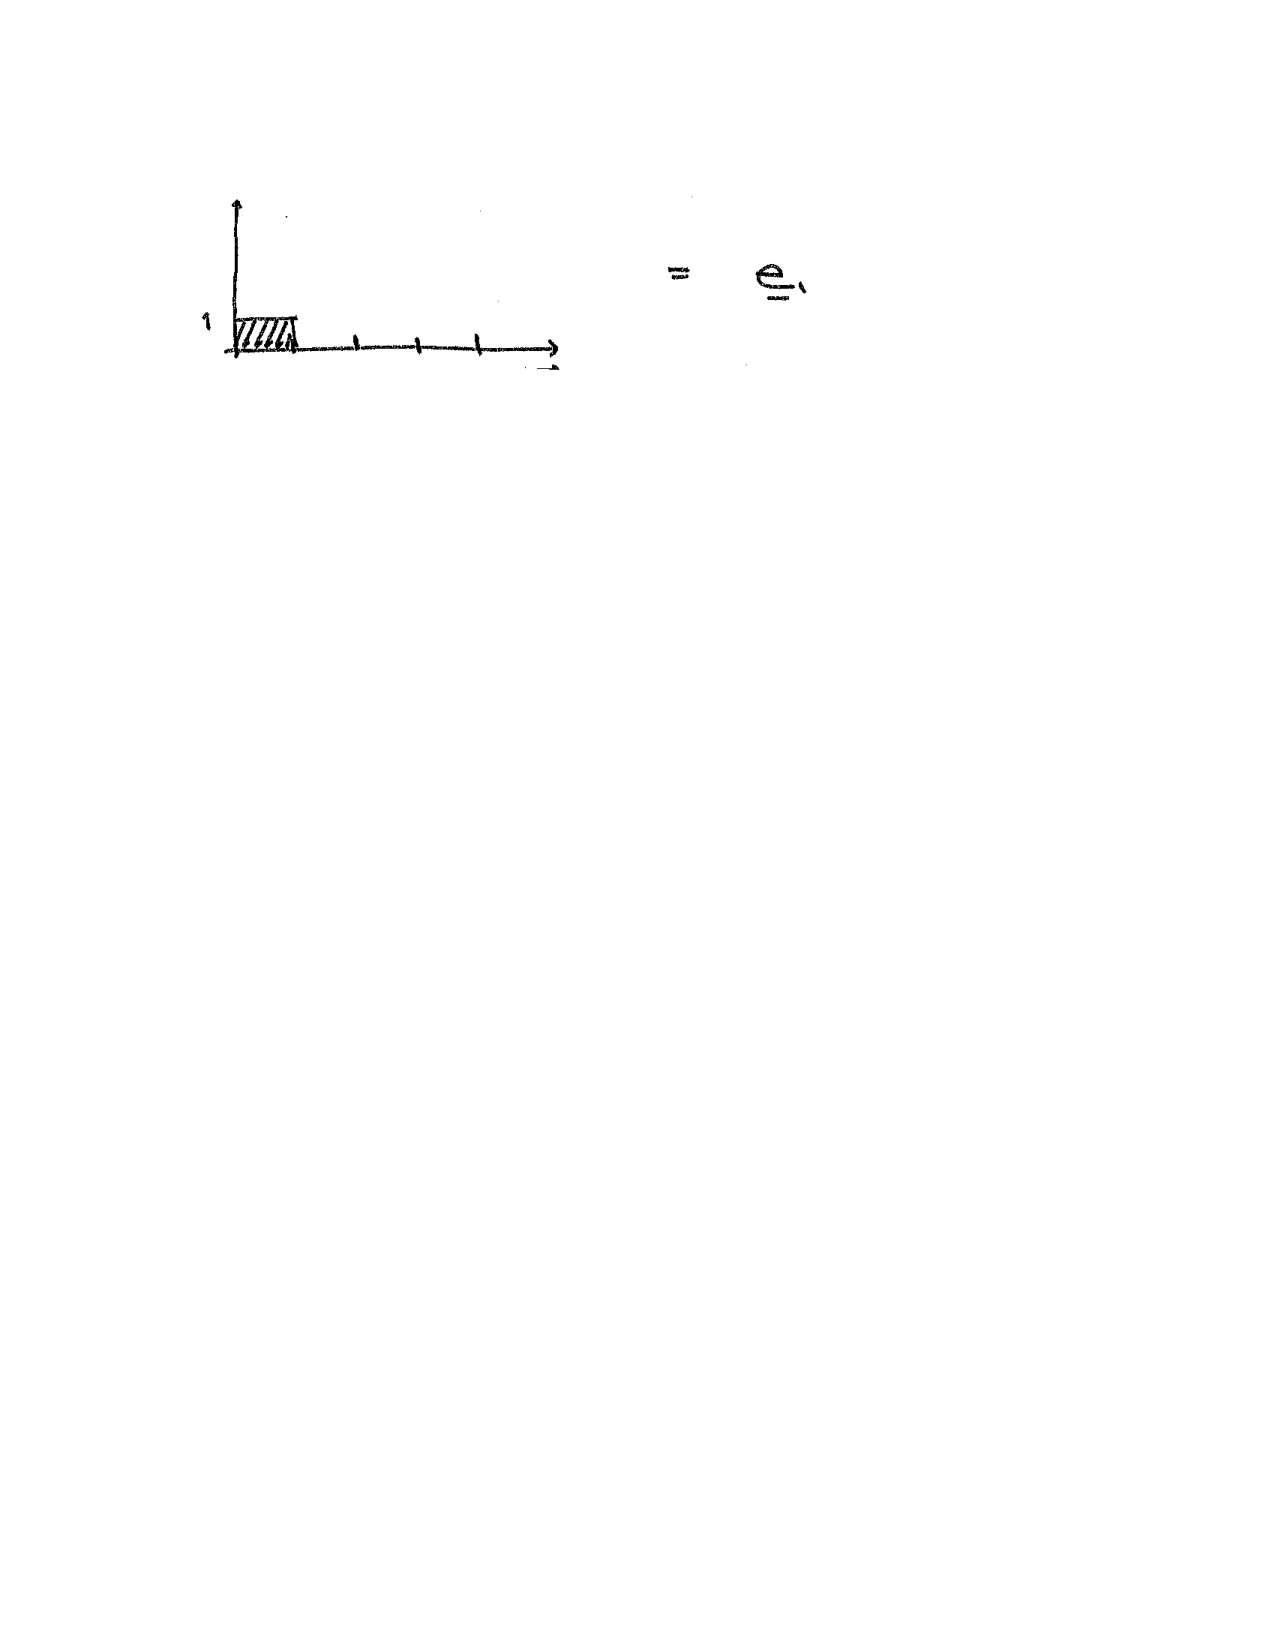
\includegraphics[width=.45\textwidth]{figures/lec02_e1.pdf}
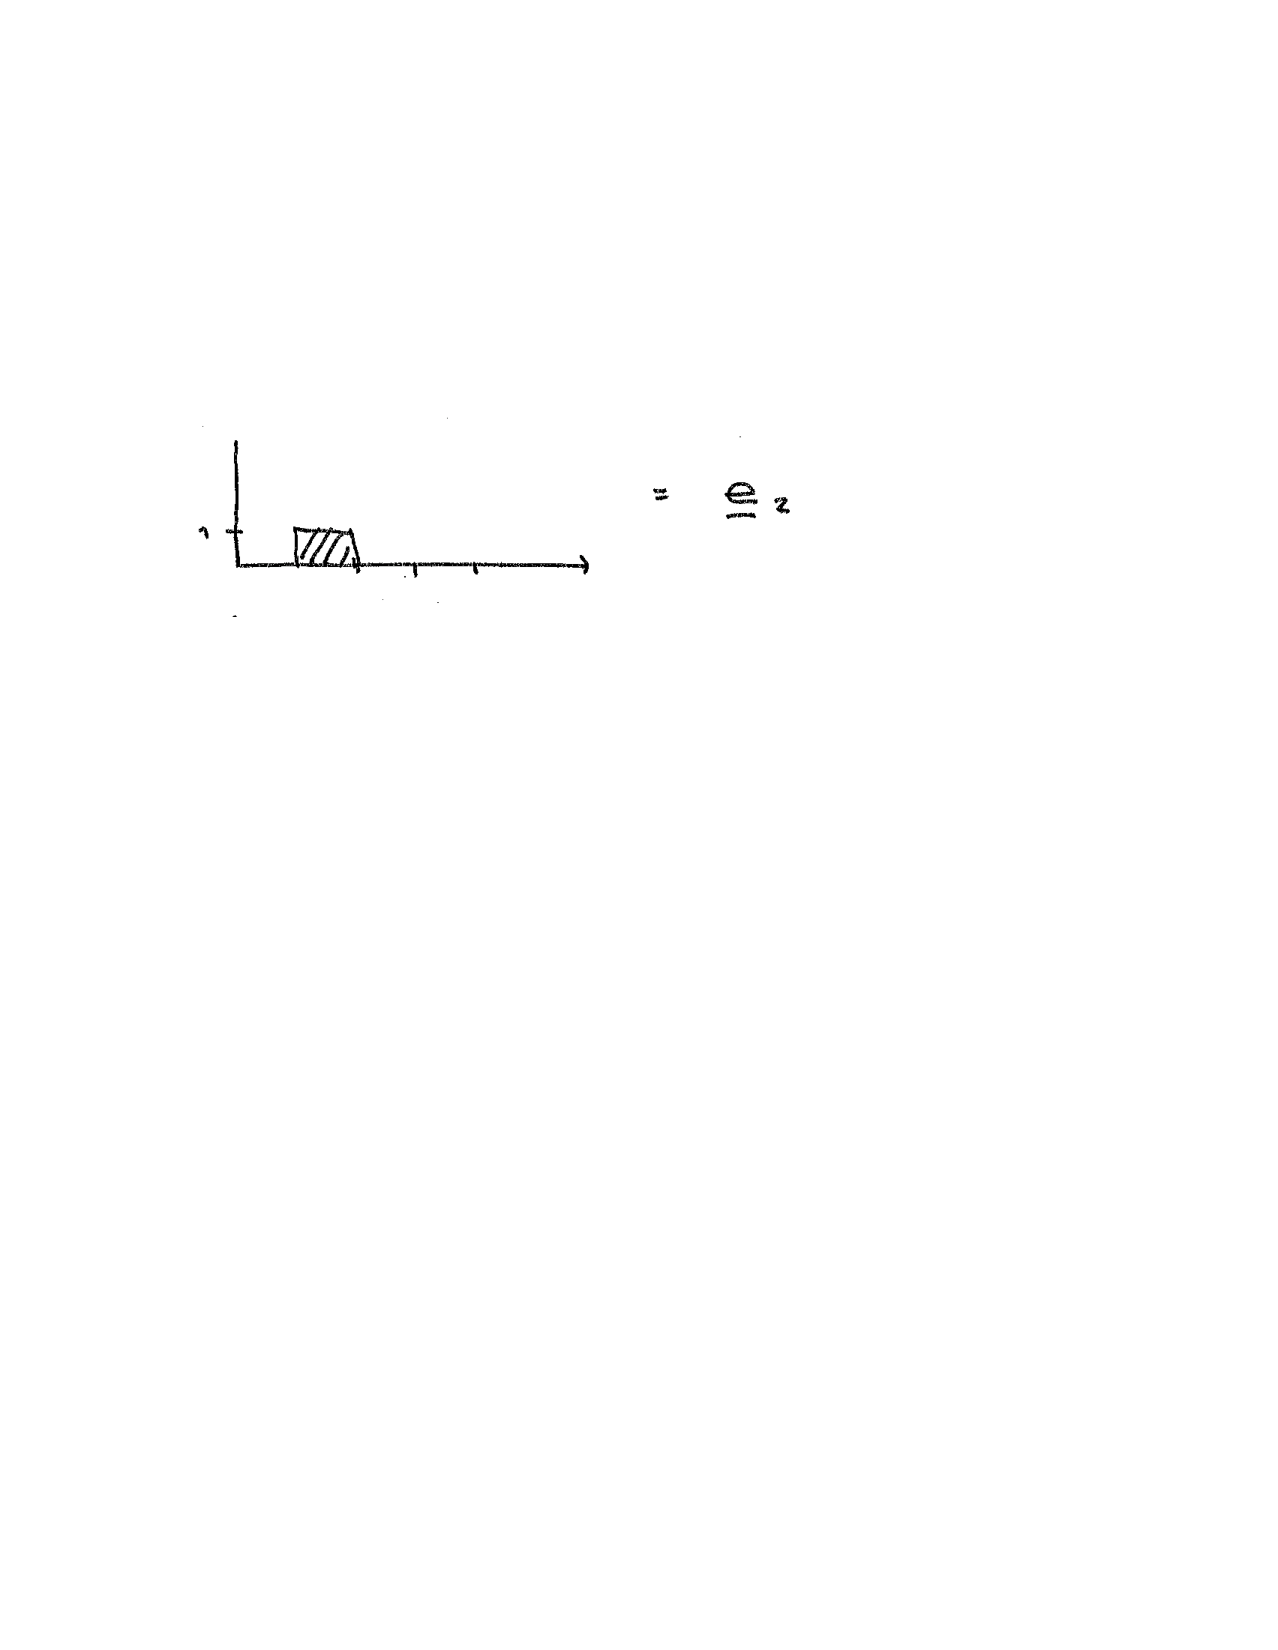
\includegraphics[width=.45\textwidth]{figures/lec02_e2.pdf}\\
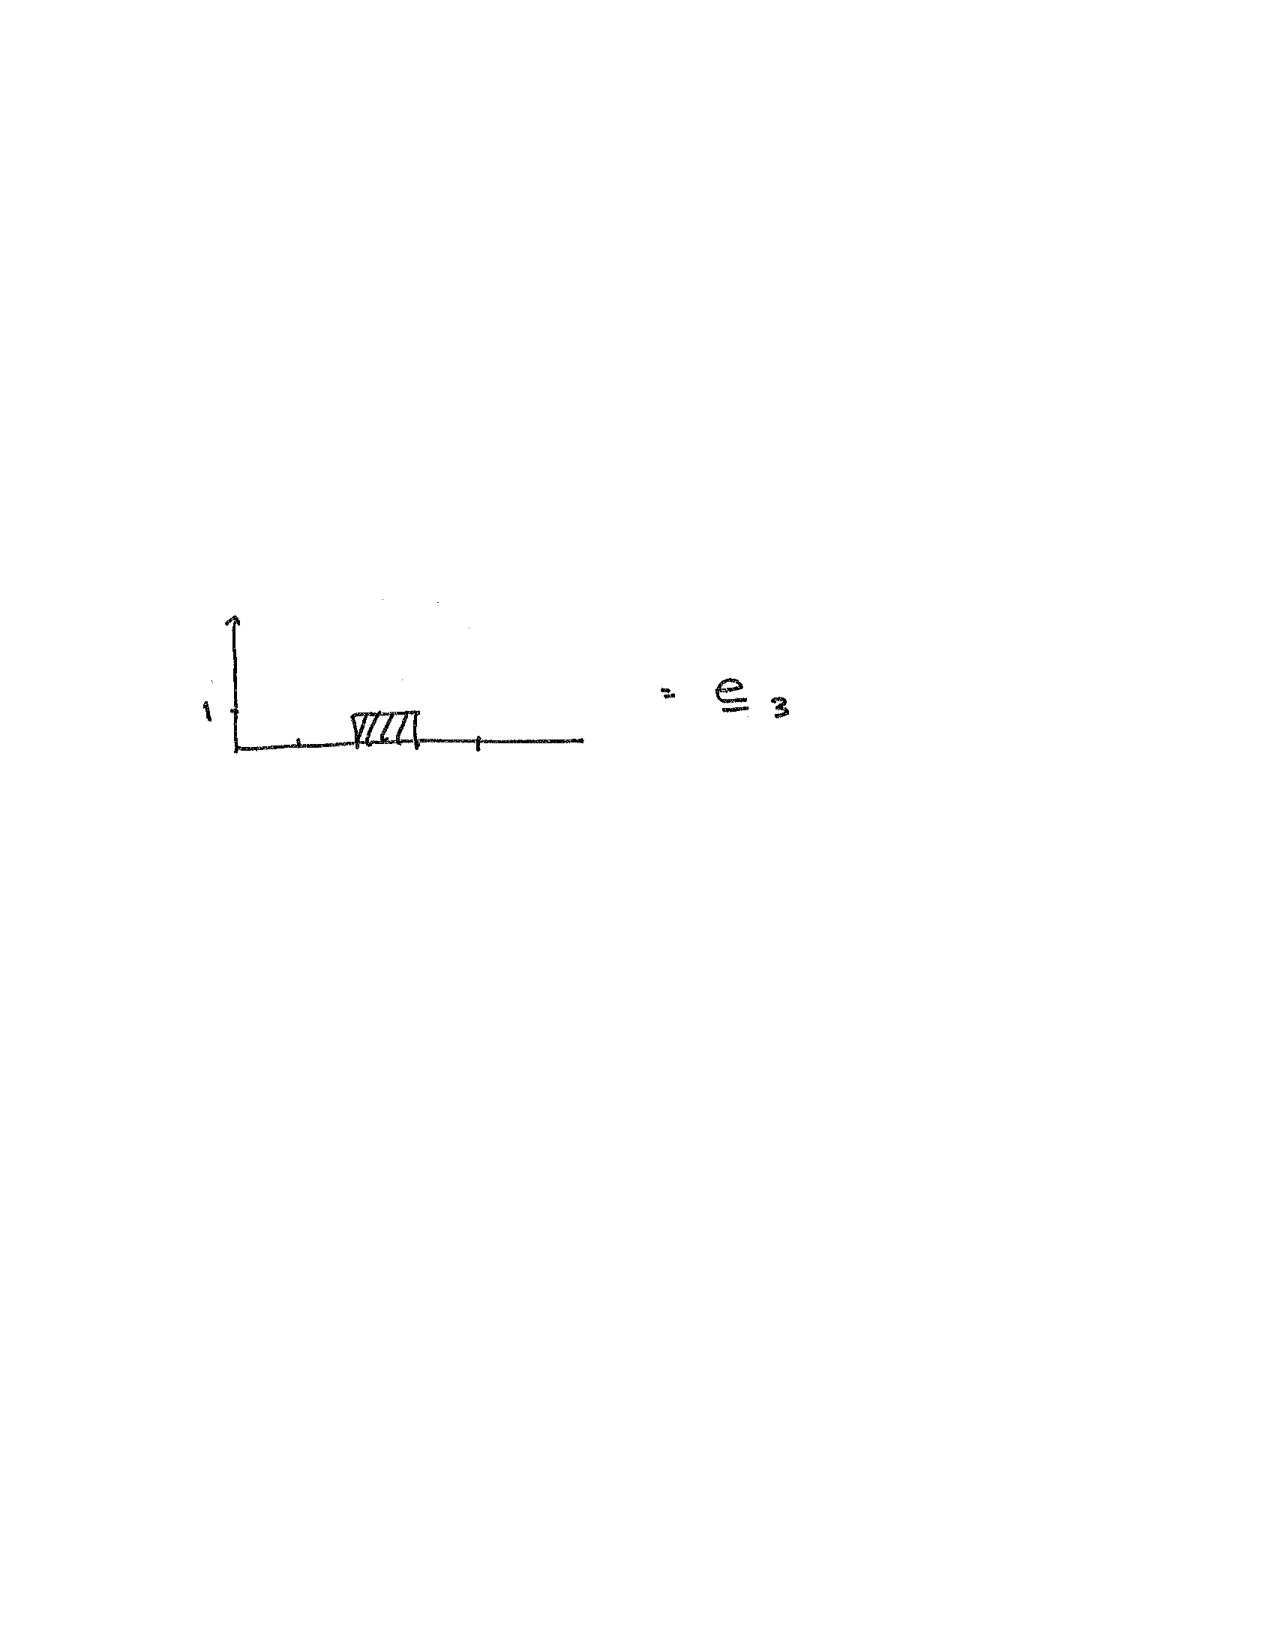
\includegraphics[width=.45\textwidth]{figures/lec02_e3.pdf}
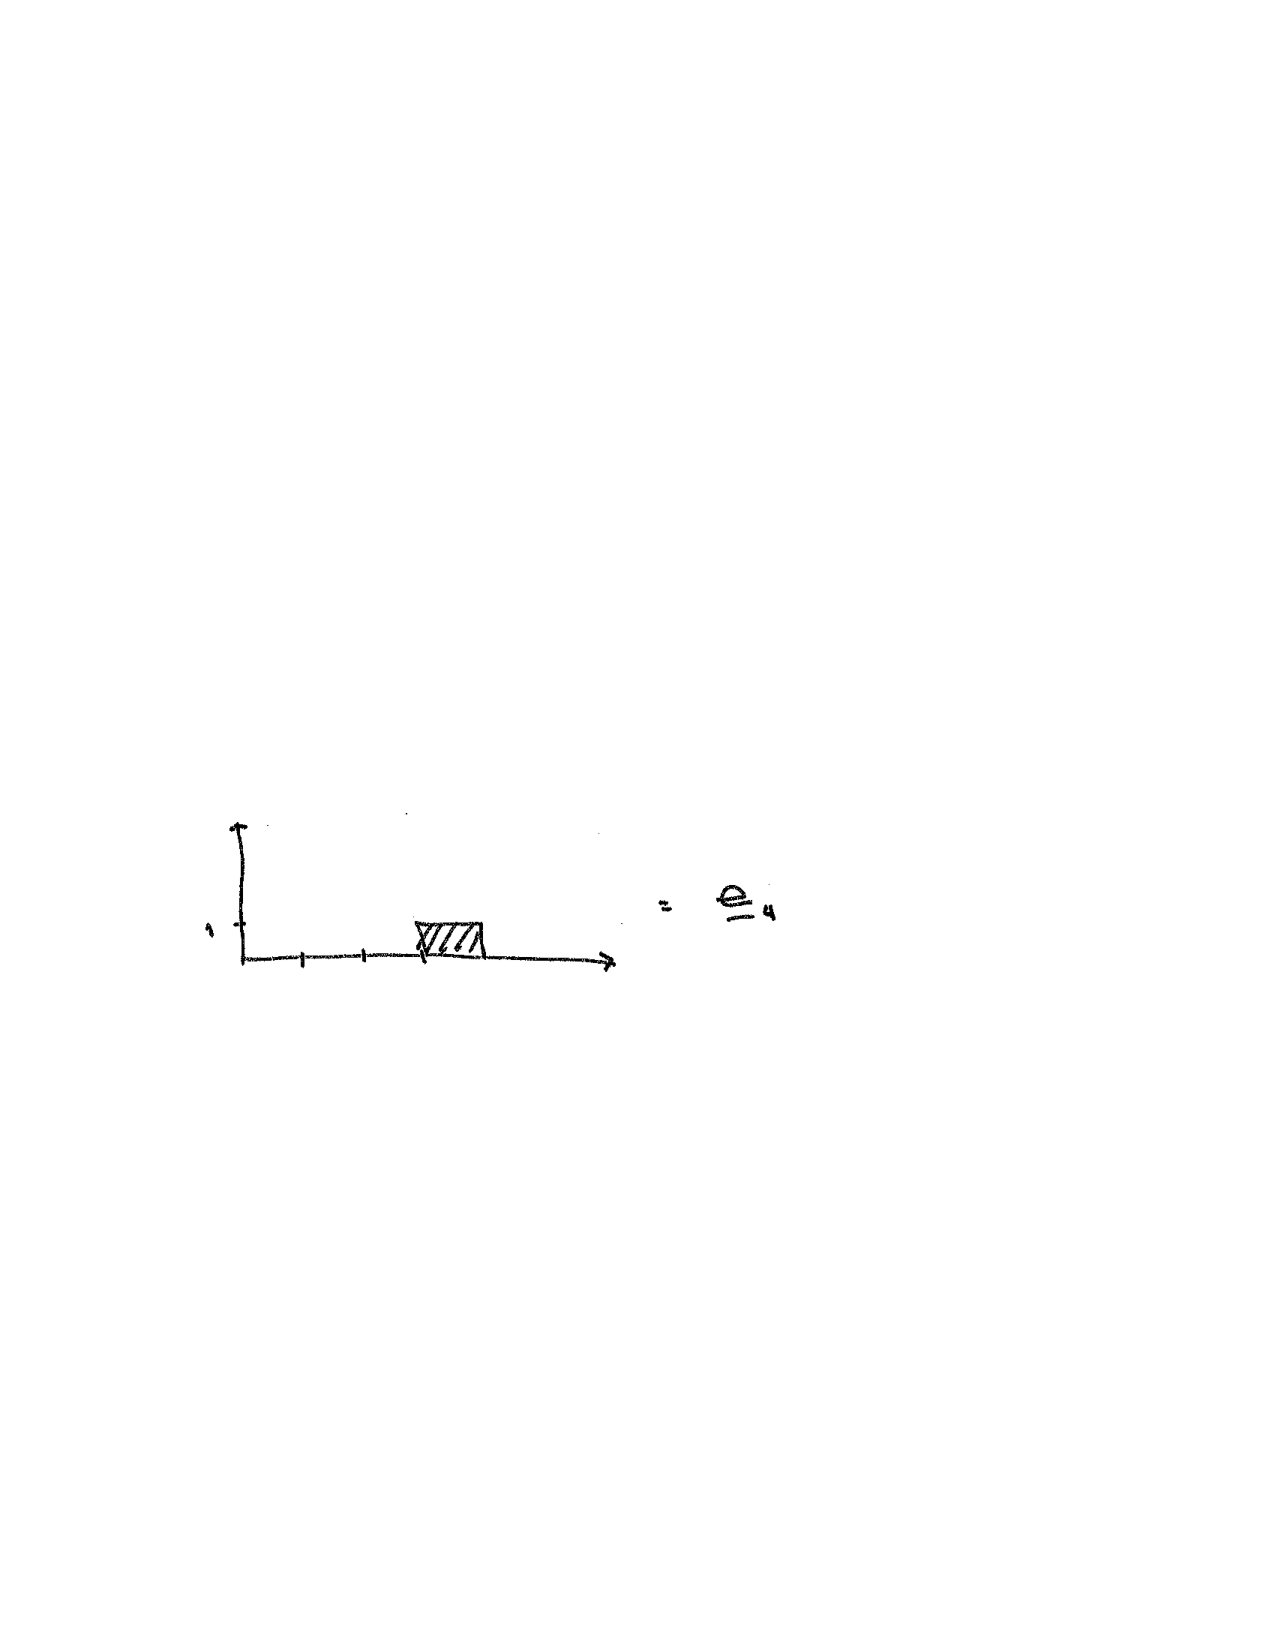
\includegraphics[width=.45\textwidth]{figures/lec02_e4.pdf}
\end{center}

\noindent This is a basis for a histogram over unit bins from $x=0$ to $x=4$. A vector in this space is, for example:

\begin{center}
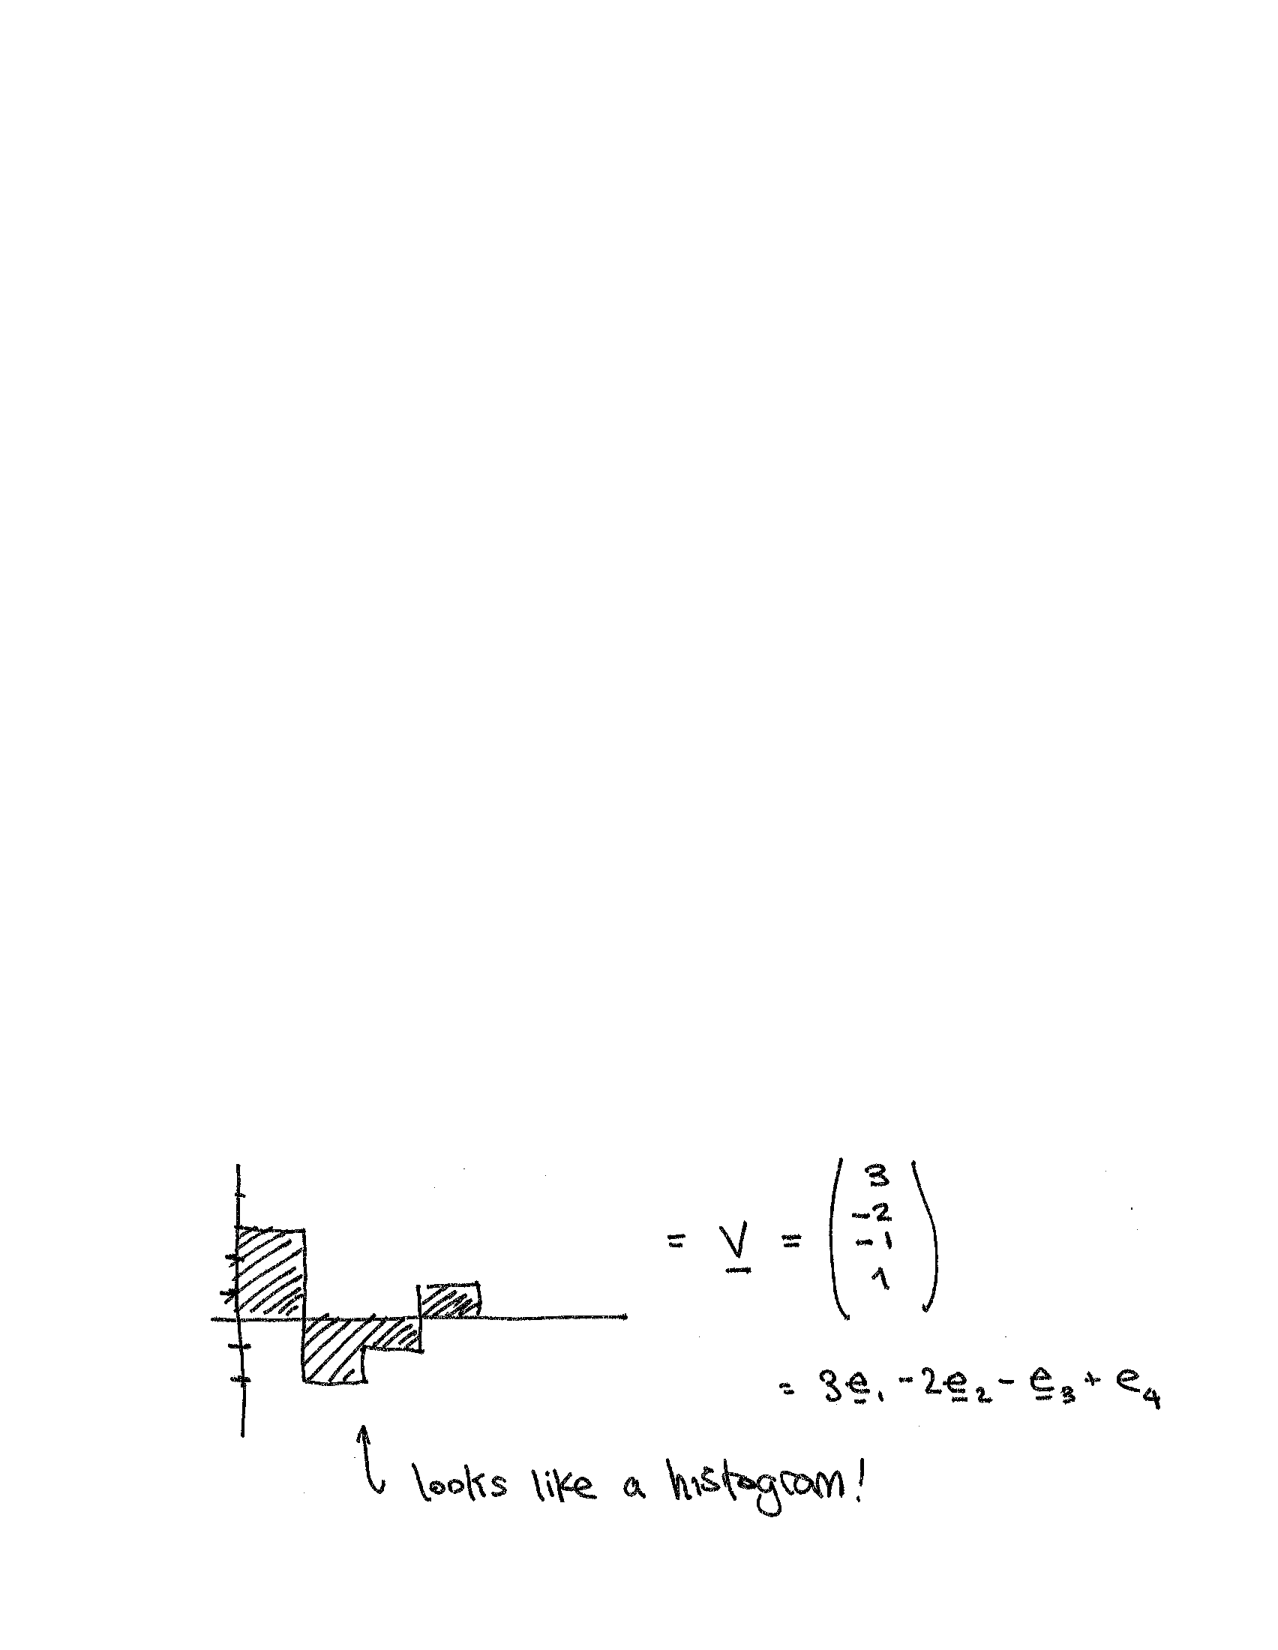
\includegraphics[width=.8\textwidth]{figures/lec02_hist.pdf}
\end{center}

\noindent We can perform a linear transformation $A$ on $\vec{v}$ which outputs another vector. Let’s say it’s this:


\begin{center}
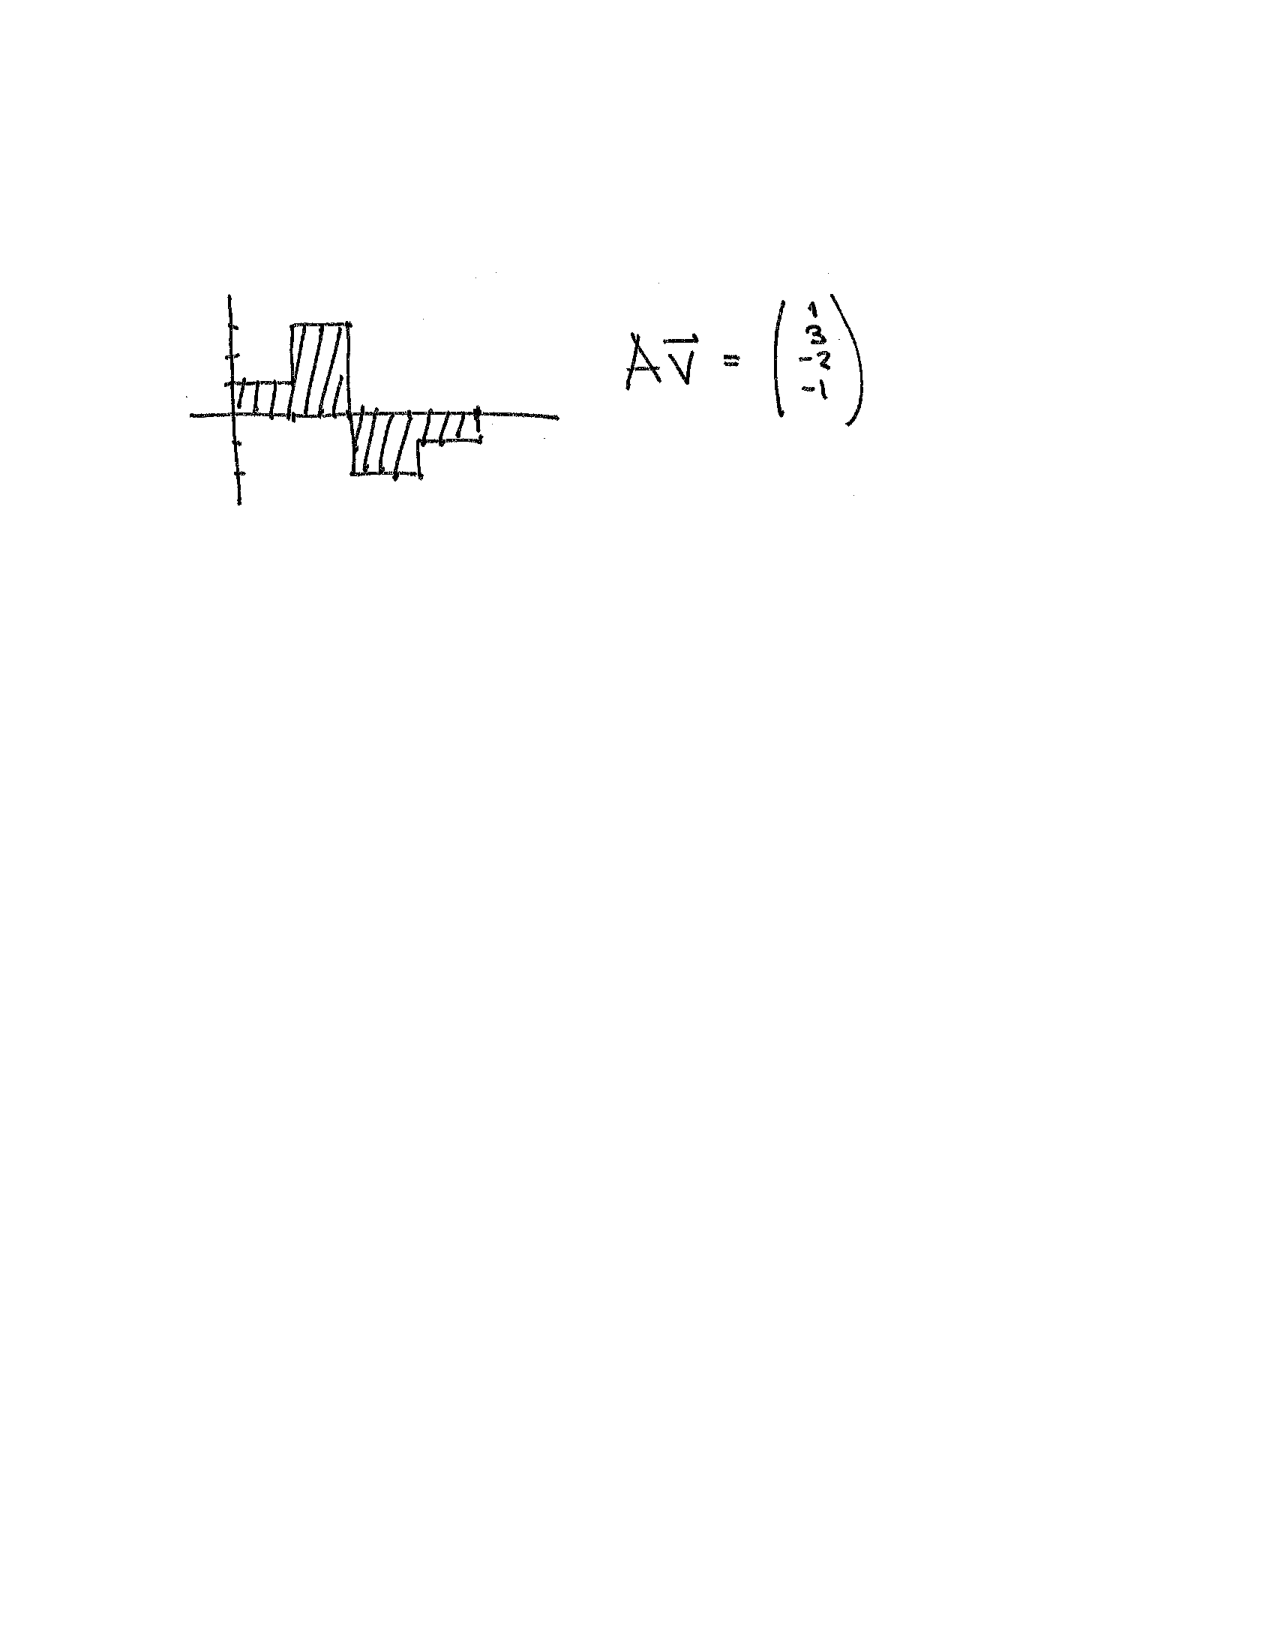
\includegraphics[width=.8\textwidth]{figures/lec02_hist2.pdf}
\end{center}

\begin{exercise}
From the image above, can you derive what $A$ is? 
\end{exercise}

\noindent The answer to the above exercise is \emph{no}. Please make sure you convince yourself why: there are many different transformations that convert to old histogram into the new histogram. If you're not convinced: the matrix $A$ is $4\times 4$ and thus has 16 entries that we need to define. The matrix equation $A\vec{v} = \vec{w}$ for known vectors $\vec{v}$ and $\vec{w}$ encodes only four equations.

The power of this admittedly strange formalism is that we can think of these histograms as approximations of continuous functions:

\begin{center}
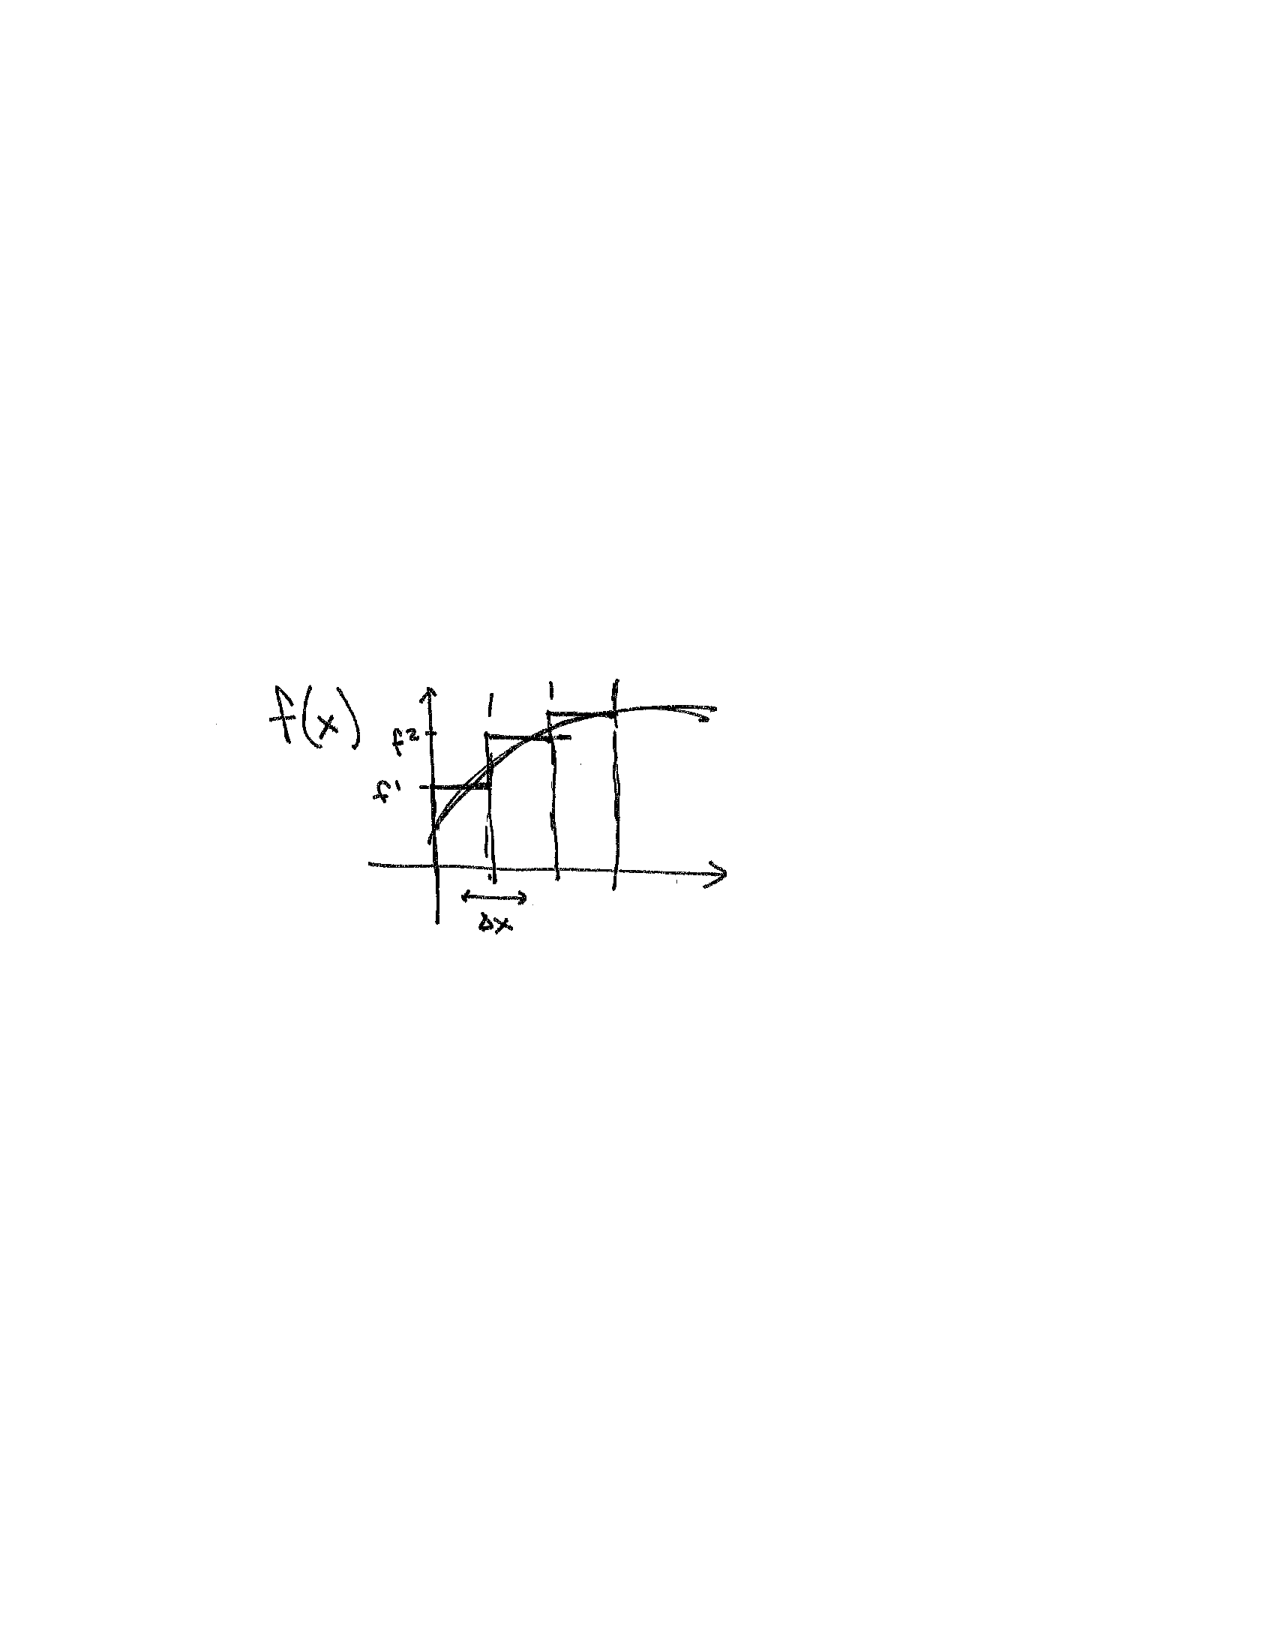
\includegraphics[width=.4\textwidth]{figures/lec02_histfun.pdf}
\end{center}

Thus a vector in this approximate (discretized) \emph{function} space is 
\begin{align}
  \vec{f} = 
  \begin{pmatrix}
    f^1 \\
    f^2 \\
    \vdots\\
    f^N
  \end{pmatrix} \ .
\end{align}

%% TO INCLUDE: why the historgram basis is dumb
%% I had some good reference for this from P17
%% ... perhaps Linear Algebra done right, or Appel or Cahill...
%% ... the point was convergence.


In what way are polar coordinates an orthonormal basis? 


\section{Linear Transformations}

\subsection{Derivative Operators}

Our discretized function space allows us to define a [forward] derivative\footnote{One could have also defined a backward derivative where $(f')^i \sim f^{i}-f^{i-1}$ \ . Note that you \emph{cannot} try to make this symmetric by defining a `centered' derivative like $(f')^i \sim f^{i+1/2}-f^{i-1/2}$ because there's no such thing as a fractional index. If you tried to write $(f')^i\sim f^{i+1}-f^{i-1}$ you're making a worse approximation. If you're like me, the fact that there's some asymmetry in how we define the first derivative is deeply unsettling. There's something to this intuition!}:
\begin{align}
  \vec{f'} =
  \frac{1}{\Delta x}
  \begin{pmatrix}
    f^2 - f^1 \\
    f^3 - f^2 \\
    \vdots
    \\
    f^{i+1}-f^i
    \\
    \vdots
  \end{pmatrix} \ .
\end{align}
This is familiar if you’ve ever had to manually program a derivative into a computer program. Note that the right-hand side looks like a linear transformation of $\vec{f}$. In other words, we expect to be able to write a matrix $D$ so that
\begin{align}
  \vec{f'} = D\vec{f} \ .
\end{align}
One problem is apparent: what happens at the `bottom’ of the vector? What is the last component of the derivative, $\vec{f'}^N$? Formally, this is
\begin{align}
  {(f')}^N = \frac{1}{\Delta x}(f^{N+1} - f^N) \,
\end{align}
but now we have no idea what $f^{N+1}$ is. That was never a component in our vector space. There is no $\vec{e}_{(N+1)}$ basis vector. 
%
This demonstrates and important lesson that we’ll need when we move more formally to function spaces:
\begin{quote}
\textbf{Boundary conditions are part of the definition of the function space}.   
\end{quote}
That was so important that I put the whole damn sentence in boldface and set it in the middle of the line. The significance of boundary conditions may be a bit surprising---but think of this as part of the definition of which functions we allow into our function space. 
%
\begin{example}
When one first learns about Fourier series with Dirichlet boundary conditions, one finds that the Fourier expansion \emph{only} contains sines. The solution to the wave equation in such a system is some function that is zero at each endpoint. So the function space relevant to the system is composed only of functions that are zero at each endpoint.
\end{example}
%
For now let us assume \textbf{Dirichlet boundary conditions}.\index{Dirichlet} A convenient way to impose this is to define what happens to all functions outside the domain of the function space:
\begin{align}
  f^{i > N} = f^{i < 1} = 0 \ .
\end{align}
This solves the problem of the derivative on the last component:
\begin{align}
  {(f')}^N = \frac{1}{\Delta x}(f^{N+1} - f^N) 
  = 
  \frac{- f^N}{\Delta x}  \ .
\end{align}
Alternatively, we could have also imposed \textbf{periodic boundary conditions}\index{periodic}:
\begin{align}
  f^{i} &= f^{i+ kN}
  & k\in \mathbb{Z} \ .
\end{align}
This would then give
\begin{align}
  {(f')}^N = \frac{1}{\Delta x}(f^{N+1} - f^N) 
  = 
  \frac{1}{\Delta x}(f^{1} - f^N) 
  \ .
\end{align}
Periodic boundary conditions amount to wrapping the $x$-axis into a circle. Older folks sometimes call this \emph{Asteroids} boundary conditions. I'd also accept \emph{Star Control} boundary conditions. Periodic boundary conditions show up \emph{all} the time in physics. Sometimes they show up in obvious places, like the Brillouin zone of a crystal lattice. Other times they show up in not-so-obvious places like the boundary conditions of the known universe. In addition to being crucial for a well-defined function space, the boundary conditions of a system establish its topology\footnote{I cannot over-emphasize the importance of topology in contemporary physics. Most of the physics you will learn in your first year graduate courses are intrinsically \emph{local} because the laws of physics are causal. Topological quantities are \emph{global}, they are integrals over an entire space. Because winding numbers (and their higher-dimensional cousins) are quantized, they are robust against perturbations. The number of holes in a donut is one, whether or not it's been slightly squished in the box. By the way, the best donuts in Southern California are from \emph{Sidecar Doughnuts} in Costa Mesa. Get the Basil Eggs Benedict donut before 11am; you can thank me later.}.

\begin{exercise}
We don't know anything about the universe outside the Hubble radius. Why do you think it would be reasonable in a physical model to \emph{assume} that it has periodic boundary conditions? Hint: what would happen to the $x$-momentum of an asteroid in the classic arcade game \emph{Asteroids} if the game did not have periodic boundary conditions? 
\end{exercise}

The second derivative may be defined symmetrically:
\begin{align}
  (f'')^i = \frac{(f^{i+1} - f^i) - (f^i - f^{i-1})}{\Delta x^2} \ .
\end{align}
You may pontificate about the reason why the first derivative does have a symmetric discretization while the second derivative does. 


\section{Why histogram space is dumb}
\label{sec:histogram:space:is:dumb}

The notion of building up continuous functions $f(x)$ from the histogram basis above turns out to be problematic from the point of view of mathematical rigor. You can read more about the problems in Appel, \emph{Mathematics for Physicists} Chapter 9.1 (Insufficiency of Vector Spaces), or Hassani, \emph{Mathematical Physics}, Chapter 7 (Hilbert Spaces). The problem in an infinite dimensional vector space is that one can take a convergent sequence of vectors whose limiting vector is not part of the vector space. This has to do with the definition of a norm of a vector with an infinite number of terms. Our histogram space is a vector space with a good inner product: this is called a \textbf{pre-Hilbert space}\index{pre-Hilbert space}. An infinite dimensional vector space that \emph{does} contain all of its limits\footnote{Formally this means that any sequence of points that progressively become arbitrarily close to each other (a Cauchy sequence) converges to a point that is also in the space.} (it is complete) is called a \textbf{Hilbert space}\index{Hilbert space}.

\flip{To do: show why the histogram space fails the Cauchy sequence test.}


\section{Derivatives in other function space bases}
\label{sec:derivatives}

There are other ways to write a discrete basis of functions. Here is a natural one for functions that are up to second-order polynomials:
\begin{align}
  \vec{e}_{(0)} &= 1
  &
  \vec{e}_{(1)} &= x
  &
  \vec{e}_{(2)} &= x^2 \ .
\end{align}
Let’s sidestep questions about orthonormality for the moment. Clearly linear combinations of these basis functions can produce any quadratic function:
\begin{align}
  f(x) &= a x^2 + bx + c
  & \Rightarrow&&
  \vec{f} &=
  \begin{pmatrix}
     c \\ b \\ a
   \end{pmatrix} \ . 
\end{align}
The derivative operator has an easy representation in this space:
\begin{align}
  D = 
  \begin{pmatrix}
    0 & 1 & 0   \\
    0 & 0 & 2   \\
    0 & 0 & 0   
  \end{pmatrix} \ .
\end{align}
We can see that
\begin{align}
  D \vec{f}  &= 
  \begin{pmatrix}
     b \\
     2 a \\
     0
  \end{pmatrix} 
  &
  D^2 \vec{f}  &= 
  \begin{pmatrix}
     2a \\
     0 \\
     0
  \end{pmatrix} 
  &
  D^3 \vec{f}  &= 
  0 \ .
\end{align}
The last line is, of course, the realization that the third-derivative of a quadratic function vanishes. Feel free to attach mathy words to this like \emph{kernel}.\footnote{Unfortunately `kernel' is also used when discussing probability distributions. To the best of my knowledge the two usages are completely independent.}

There are other bases that we may use for function space. A particularly nice one that we will use over and over is the Fourier basis, which we usually refer to as \emph{momentum space}. The basis vectors are things like sines, cosines, or oscillating exponentials. These do not vanish for any power of $D$.


\section{Locality}

Notice that in the histogram basis, the derivative matrix $D$ is sparse: it is zero everywhere away from the diagonal. The only non-zero elements on the $i^\text{th}$ row are around the $(i\pm 1)^\text{th}$ column.  Higher powers of $D$ sample further away, but the non-zero elements are always clustered near the diagonal.

This is simply a notion of \textbf{locality}. Remember the Taylor expansion:
\begin{align}
  f(x) = f(0) + f'(0) x + \frac{1}{2} f''(0)x^2 + \cdots \ .
\end{align}
If we think about the histogram as a discretization of a continuous function, then it is clear what the higher derivatives are doing. Given a function $f(x) = \vec{f}$, one might like to know about the function around some point $x_0$ corresponding to some index $i$. That is: $f^i = f(x_0)$. If you’d like to learn more about the function around that point, one can express the derivative at $x_0$. Thus $D\vec{f}$ says something about the slope, $D^2\vec{f}$ says something about the curvature, and so on. Because each successive power of $D$ samples terms further away from $f^i$, you can tell that these higher order terms are learning about the function further and further away from $x_0$. 

Now think about the types of differential equations that you’ve encountered in physics. They often include one or two derivatives. You hardly ever see three, four, or more derivatives\footnote{With some thought, it may also be clear why spatial derivatives typically appear squared.}. There’s a reason for this: at the scales that we can access experimentally, nature appears to be local. Our mathematical models of nature typically have locality built in\footnote{A recent counterexample ``A Jewel at the Heart of Quantum Physics,'' by Natalie Wolchover in \emph{Quanta Magazine} (2013).
% https://www.quantamagazine.org/physicists-discover-geometry-underlying-particle-physics-20130917/
}. Physics at one spacetime point should not depend on spacetime points that are far away. 

This may be familiar from the idea of causality---the idea that $A$ \emph{causes} $B$ therefore $A$ must have happened \emph{before} $B$. One of the key results in special relativity is that causality can be tricky if two events do not occur at the same spacetime point. More carefully, $A$ can only cause $B$ if there is a timelike separation of the appropriate sign.  If we want to build causal theories of nature, then the dynamics at $x_0$ should not rely on what is happening at $x_1$, a finite distance away.\footnote{This is different from saying that information cannot propagate from $x_0$ to $x_1$; such propagation could come from some causal excitation of the electromagnetic field traveling every infinitesimal distance between the two positions. This is reminiscent of the classical Zeno's paradox.}

\section{The Green's Function Problem in Function Space}

The Green's function can be defined by analogy to the finite-dimensional inverse transformation. The finite-dimensional linear system $A\vec v = \vec w$ can be solved by applying the inverse transformation $A^{-1}$ in the same way that the continuum (infinite-dimensional) system $\mathcal O \psi(x) = s(x)$ can be solved with the Green's function $G(x,y)$ of the operator $\mathcal O$:
\begin{align}
  v^i &= \sum_i 
  \mat{\left(A^{-1}\right)}{i}{j} w^j
  &\Rrightarrow
  &
  &
  \psi(x) &= \int  dy\, G(x,y) s(y) \ .
  \label{eq:def:of:function:space:Greens:function}
\end{align}
We've explicitly written out the sum over the dummy index $i$ to emphasize the analogy to the integration over the dummy variable $y$. The arguments of the functions play the role of `continuum indices.'

\section{Differential Operators}

Linear transformations on function space are differential operators. In principle you can imagine linear transformations that are not differential operators, for example a finite translation. However, because our models of nature are typically \emph{local} and \emph{causal}, the linear transformations that we obtain from physical models are differential operators\footnote{This is not to say that finite transformations are somehow not permitted. The dynamics that govern our models of nature, however, only dictate how information is transmitted infinitesimally in space and time. Propagation forward in time by some finite interval is described by the exponentiation of infinitesimal forward time translations. This is, of course, why the time-translation operator in quantum mechanics is $e^{i\hat H t}$, where the Hamiltonian $H$ is described as a local function with perhaps one or two derivative operators.}. 

Let's write a general differential operator as:
\begin{align}
  \mathcal O = 
  p_0(x) 
  + p_1(x) \frac{d}{dx}
  + p_2(x) \left(\frac{d}{dx}\right)^2
  + \cdots
  \label{eq:differential:operator}
\end{align}
where the $p_i(x)$ are polynomials. Sometimes we will write this as $\mathcal O_x$ to make it clear that the argument of the polynomials is $x$ and the variable with which we are differentiating is $x$.  
\begin{exercise}
Explain why \eqref{eq:differential:operator} is a linear operator acting on function spaces.
\end{exercise}
\begin{exercise}
A confused colleague argues to you that \eqref{eq:differential:operator} cannot possibly be `linear.' Just look at it, your colleague says: the functions $p_i(x)$ are polynomials---those aren't \emph{linear}! There are also powers of derivatives---how is that possibly linear? Explain to your colleague why the $p_i(x)$ does not have to be linear nor is one restricted to finite powers of derivatives for the operator $\mathcal O$ to be a linear operator acting on function space.
\end{exercise}
Technically \eqref{eq:differential:operator} is called a \textbf{formal operator} because we haven't specified the boundary conditions of the function space. Recall in our discretized `histogram space' in Section~\ref{sec:histogramspace} that we had to be careful about how to define the derivative acting on the boundaries of the space. A differential operator along with boundary conditions is called a \textbf{concrete operator}.

\section{Inner Product}

There's a convenient inner product that you may be familiar with from quantum mechanics. For two functions $f(x)$ and $g(x)$ in your function space, define the inner product to be
\begin{align}
  \langle f,g\rangle 
  =
  \int dx\, f^*(x)g(x) \ .
  \label{eq:L2:inner:product}
\end{align}
\begin{example}
Wave functions in 1D quantum mechanics obey this norm. For an infinite domain, we typically restrict to square-integrable functions meaning that $|f|^2$ goes to zero fast enough at $\pm \infty$ so that the integral $\langle f, f\rangle$ is finite. 
\end{example}
Sometimes the inner product is defined with respect to a \textbf{weight} function $w(x)$:
\begin{align}
  \langle f,g\rangle_w 
  =
  \int dx\, w(x)\, f^*(x)g(x) \ .
  \label{eq:weighted:inner:product}
\end{align}
There's nothing mysterious about inner products with weights. They typically boil down to the fact that one is not using Cartesian coordinates. 
\begin{example}
Have you met the Bessel functions? If not, you're in for a treat in your electrodynamics course. The Bessel functions satisfy a funny orthogonality relation with weight $w(x)\sim x$ because they show up as the radial part of a solution when using polar coordinates. When you separate variables, $d^2x = rdr\,d\theta$, we see that the measure over the radial coordinate $r$ carries a \emph{weight} $r$.
\end{example}
We will assume unit weight until we go to higher spatial dimensions\footnote{My dissertation focused on theories of extra dimensions. I also noticed that my weight increased in my final year of graduate school as I spent most of my time writing about extra dimensions and eating cafe pastries.}.


\section{Dual Vectors}

What are the `dual functions' (dual vectors, bras) in function space? These are linear functions on act on functions and spit out numbers. These are integrals that are pre-loaded with some factors. Assuming unit weight:
\begin{align}
  \langle f | = \langle f, \qquad \rangle
  = 
  \int dx \, f^*(x) \left[\text{ insert ket here }\right] \ .
\end{align}



\section{Adjoint operators}

What is the adjoint of a differential operator? The definition of the adjoint \eqref{eq:def:adjoint} and the function space inner product \eqref{eq:L2:inner:product} give us a hint. We define $\mathcal O^\dag$ by the property
\begin{align}
  % \int dx \, \left[\mathcal O f(x)\right]^* g(x)
  % = 
  % \int dx \, f^*(x) \left[\mathcal O^\dag g(x)\right] \ .
  \int dx \, f(x)^* \left[\mathcal O g(x)\right]
  \equiv
  \int dx \, \left[\mathcal O^\dag f(x)\right]^*  g(x) \ .
\end{align}
The strategy is: given an inner product (integral) over $f^*$ and $g$ where there is some stuff ($\mathcal O$) acting on $g$, can we re-write this as an integral with no stuff acting on $g$ and some \emph{other} stuff acting on $f^*$? If so, then the `other stuff' is the adjoint $\mathcal O^\dag$.
\begin{example}
What is the adjoint of the derivative operator, $\mathcal O = d/dx$? Assume an interval $x\in[a,b]$ and Dirichlet boundary conditions, $f(a)=f(b)=0$. There's a simple way to do this: integrate by parts.
% \begin{align}
%   \int dx \, \left[\frac{d}{dx} f(x)\right]^* g(x)
%   =
%   - \int dx \, f^*(x) \left[\frac{d}{dx}g(x)\right]
%   +
%   \left[f^*(x)g(x)\right]^b_a \ 
%   =
%   - \int dx \, f^*(x) \left[\frac{d}{dx}g(x)\right] \ . 
% \end{align}
\begin{align}
  \int dx \,  f(x) \left[\frac{d}{dx} g(x)\right]
  =
  - \int dx \, \left[\frac{d}{dx}f(x)\right]^* g(x)
  +
  \left[f^*(x)g(x)\right]^b_a \ 
  =
  \int dx \, \left[-\frac{d}{dx}f(x)\right]^* g(x)
  \ . 
\end{align}
From this we deduce that
\begin{align}
  \left(\frac{d}{dx}\right)^\dag = -\frac{d}{dx} \ .
\end{align}
\end{example}

We will be especially interested in \textbf{self-adjoint} (Hermitian) operators for which
\begin{align}
  \mathcal O^\dag = \mathcal O \ .
\end{align}
This is, as we mentioned for the finite-dimensional case, because self-adjoint operators are \emph{nice}: they have real eigenvalues and orthogonal eigenvectors. Since most physical values are real eigenvalues of some operator, one may expect that the differential operators that show up in physics are typically self-adjoint.
\begin{exercise}
We saw above that the derivative operator is not self-adjoint. What is an appropriate self-adjoint version of the derivative operator? \emph{Hint: what is the momentum operator in quantum mechanics?}\footnote{\url{https://aapt.scitation.org/doi/abs/10.1119/1.9932}} 
\end{exercise}
\begin{example}
Consider $\mathcal O = -\partial_x^2$ defined on the domain $x\in [0,1]$ with the boundary conditions $f(0)=f(1)=0$. Is this operator self-adjoint? We want to check of $\langle f,\mathcal O g\rangle = \langle O f, g \rangle$. We have one trick: integration by parts. Let's see how this works.
\begin{align}
  \langle f, \mathcal O g\rangle &= - \int dx\, f^*(x)\partial^2 g(x) \ .
\end{align}
This is compared to
\begin{align}
  \langle \mathcal O f, g\rangle 
  &= -\int^1_0 dx\, \left[\partial^2 f(x)\right]*g(x) 
  \\
  &= 
  -\left.\left(\partial f(x)\right)^*g(x)\right|^1_0
  + \int^1_0 dx \, \left[\partial f(x)\right]^* \partial g(x) 
  \\
  &= \left.f^*(x)\partial^2 g(x)\right|^1_0
  - \int^1_0 dx \, f^*(x) \partial^2 g(x)  
  \\
  &=
  - \int^1_0 dx \, f^*(x) \partial^2 g(x)  
  \ .
\end{align}
And so we see that indeed $(-\partial^2)^\dag = -\partial^2$.
\end{example}
\begin{exercise}
In the previous example, what is the significance of the overall sign of the operator? \emph{Hint: the sign doesn't matter, it's because we typically think of $-\partial^2$ and its higher-dimensional derivatives as the square of the momentum operator.}
\end{exercise}
\begin{example}\label{ex:eigenfunction:fourier}
The \textbf{eigenfunctions} $f_n$ of $-\partial^2$ defined on $x\in [0,1]$ with Dirichlet boundary conditions are simply 
\begin{align}
  f_n(x) &= A_n \sin(n\pi x) 
  &
  \lambda_n = - n^2\pi^2 \ ,
  \label{eq:fourier:basis:unit:interval}
\end{align}
where $\lambda_n$ is the associated eigenvalue and $A_n$ is some normalization that. These eigenfunctions are orthonormal in the following sense:
\begin{align}
  \langle f_n, f_m\rangle = \int_0^1 dx\, \sin(n\pi x)\sin(m\pi x) = \frac{A_nA_m}{2} \delta_{nm} \ ,
\end{align}
from which we deduce that the normalization is $A_n = \sqrt{2}$. That's basically all there is to know about Fourier series.
\end{example}
\begin{exercise}
What would change if we had instead assumed Neumann boundary conditions? What if we had assumed periodic boundary conditions? What about anti-periodic boundary conditions?
\end{exercise}
\begin{exercise}\label{exe:eigenfunction:fourier}
A function $g(x)$ defined on an interval $x\in [0,1]$ with Dirichlet boundary conditions can be written with respect to the Fourier basis \eqref{eq:fourier:basis:unit:interval}. In ket notation, the $n^\text{th}$ component of $g$ with respect to this basis is
\begin{align}
  g^n = \langle f_n| g\rangle \ .
\end{align}
Confirm that this is precisely what you know from Fourier series. In other words, we can decompose $g(x)$ as
\begin{align}
  g(x) &= \sum_n \langle f_n| g\rangle f_n(x)  \ .
\end{align}
\end{exercise}

\section{Completeness in Function Space}

We rarely have much to say about the unit matrix in linear algebra. However, much like when we discussed units, we can squeeze a lot out of inserting the identity in our mathematical machinations. In order to help with translate this to function space, let's review how it works in finite dimensional vector spaces. The unit matrix is $\mathbbm{1}$ and may be written:
\begin{align}
  \mathbbm{1} = \sum_i |i\rangle\langle i| \ ,
  \label{eq:unit:matrix}
\end{align}
where $|i\rangle$ and $\langle j|$ are basis (dual-)vectors. 
\begin{exercise}
Take a moment and convince yourself that \eqref{eq:unit:matrix} is true and obvious. It may be helpful to explicitly write out $|i\rangle \langle j|$ as a matrix. 
\end{exercise}
\begin{exercise}\label{ex:completeness:for:non:cartesian:basis}
Suppose you have a two-dimensional Euclidean vector space. Show that \eqref{eq:unit:matrix} is true for the basis
\begin{align}
  |1 \rangle &= 
  \frac{1}{\sqrt{2}}
  \begin{pmatrix}
  1 \\ 1
  \end{pmatrix}
  &
  |2 \rangle &= 
  \frac{1}{\sqrt{2}}
  \begin{pmatrix}
  1 \\ -1
  \end{pmatrix}
  \\
  \langle 1 | &= 
  \frac{1}{\sqrt{2}}
  \begin{pmatrix}
  1 & 1
  \end{pmatrix}
  &
  \langle 2 | &= 
  \frac{1}{\sqrt{2}}
  \begin{pmatrix}
  1 & -1
  \end{pmatrix} \ .
\end{align}
\end{exercise}
In fact, \eqref{eq:unit:matrix} defines what it means that a set of basis vectors is \textbf{complete}. You can write any vector $|v\rangle$ with respect to the basis $|i\rangle$---the components are simply
\begin{align}
  v^i = \langle i | v \rangle
\end{align}
so that 
\begin{align}
  |v\rangle = \sum_i |i\rangle \langle i | v \rangle \ ,
  \label{eq:completeness:by:inserting:1}
\end{align}
which we recognize as nothing more than `multiplying by the identity.' 
%

What does completeness look like in function space?
\begin{framed}\noindent
Let $e_{(n)}(x)$ be a set of basis functions. The basis is \textbf{complete} if
\begin{align}
  \sum_n \left[e_{(n)}(x)\right]^* e_{(n)}(y) = \delta(x-y) \ .
  \label{eq:function:space:completeness}
\end{align}
\end{framed}
Compare this \emph{very carefully} with the completeness relation \eqref{eq:unit:matrix}. The sum over $i$ in the finite-dimensional case has been relabeled into a sum over $n$ in the function space---this is just my preference\footnote{I think this is because we will deal with complex functions and I want to avoid using $i$ as an index. But if we're being honest, it's just become a habit.}. The $\mathbbm{1}$ has been replaced by a Dirac $\delta$-function, $\delta(x-y)$. Let's confirm that this makes sense. The \emph{multiply by one} completeness relation \eqref{eq:completeness:by:inserting:1} in function space is
\begin{align}
  |g\rangle 
  &= 
  \sum_n |e_{(n)}\rangle\langle e_{(n)}| g\rangle
  &
  \langle e_{(n)}| g\rangle &=
  \int dy \, [e_{(n)}(y)]^* g(y) \ .
\end{align}
We have deliberately changed the name of the integration variable to $y$ to avoid confusion; since this variable is integrated over it's simply a \emph{dummy variable} and it doesn't matter what we name it---the quantity $\langle e_{(n)}|g\rangle$ is independent of $y$ because $y$ is integrated over\footnote{By the way, this should ring a bell from our summation convention. When an upper and lower tensor index are contracted, the resulting object behaves as if it didn't have those indices: $\mat{A}{i}{j}v^j$ behaves as a vector with one upper index.}. Writing this out explicitly as functions:
\begin{align}
  g(x) &= \sum_n\left[\int dy\, e_{(n)}^*(y)g(y)\right] e_{(n)}(x) \ .
  \label{eq:complenesss:function:space:in:action }
\end{align}
The factor in the square brackets is simply $\langle e_{(n)}| g\rangle$, which is just a \emph{number}---it has no functional dependence on $x$.
If this seems unusual, please refer back to Example~\ref{ex:eigenfunction:fourier} and Exercise~\ref{exe:eigenfunction:fourier}. 

By the way, you'll often hear people (perhaps even me) say that the Dirac $\delta$ function is not strictly an \emph{function} but rather a \textbf{distribution}---this means that it only makes sense when it is integrated over. As physicists we'll sometimes be sloppy and talk about physical quantities that could be Dirac $\delta$-functions. There is \emph{never} an appropriate, measurable physical quantity that is described by a $\delta(x)$. Anything with a $\delta(x)$ is an object that was meant to be integrated over. When you imagine that a point charge density is a $\delta$-function, this is only because you will eventually integrate over it to determine the total charge. This is precisely what we saw in the charged cat in Example~\ref{eq:charged:cat}. If you ever calculate a \emph{measurable} quantity to be $\delta(x)$ check your work. If you ever find $\delta(x)^2$, then go home, it's past your bed time.

\begin{example}
One can vaguely motivate the $\delta$-function as the unit matrix by appealing to the `histogram basis' of discretized function space. In an ordinary finite-dimensional vector space, unit matrix can be written as
\begin{align}
  \mathbbm{1} = |1\rangle\langle 1 | + |2\rangle\langle 2 | + \cdots
  = \sum_{i,j}\delta_{i}^j|i\rangle\langle j| \ .
\end{align}
The Dirac $\delta$-function in histogram space is analogous to
\begin{align}
  \delta(x-x') &\to \delta_{x}^{x'}|x\rangle\langle x'| \ ,
\end{align}
where $x$ and $x'$ are discrete bins on the right-hand side. Thus for a discretized function $f = f(x_1)|x_1\rangle + f(x_2)|x_2\rangle + \cdots$, one has
\begin{align}
  \int dy\, \delta(x-y) f(y) = f(x) \longrightarrow \sum_j \delta_{x_j}^{x_i}|x_i\rangle\langle x_j| f\rangle  =  f(x_i) |x_i\rangle\ .
\end{align}
\end{example}

\section{Orthonormality in Function Space}

One should contrast the notion of completeness of a a basis this with that of \textbf{orthonormality} of the basis. Orthonormality is the statement that
\begin{align}
  \langle i | j \rangle = \delta^j_i \ .
\end{align}
Completeness has to do with the `outer product' $|i\rangle \langle i|$ while orthonormality has to do with the `inner product' $\langle i | i\rangle = \langle i, i\rangle$. The function space generalization of orthonormality is\footnote{If you're a purist, you'll note that $\delta_{nm}$ should really be written as $\delta^n_m$ because the dual basis vector has an upper index. While this may be true, I'm making the present notational choice because the object that we would call $\tilde{\vec{e}}^{(n)}$ really does contain $e_{(n)}^*(x)$, the complex conjugate of $e_{(n)}(x)$.}
\begin{align}
  \langle e_{(n)} | e_{(m)} \rangle = \int dx \, e_{(n)}^*(x) e_{(m)}(x) = \delta_{nm} \ .
  \label{eq:function:orthonormality}
\end{align}
\begin{exercise}
Why does \eqref{eq:function:orthonormality} have a Kronecker $\delta$ with discrete indices when \eqref{eq:function:space:completeness} has a Dirac $\delta$? Please make sure you can answer this; it establishes the conceptual foundation of the analogy between finite- and infinite-dimensional vector spaces.
\end{exercise}
For the completeness relation, we sum over the same eigenfunction label $n$ for a function and its conjugate evaluated at different continuous positions. For the orthonormality relation, we integrate over the positions of two different eigenfunction indices, $n$ and $m$. 

Do not confuse the eigenfunction label with the index of a vector. If this is confusing, please refer back to Exercise~\ref{ex:completeness:for:non:cartesian:basis}. You may be stuck thinking about basis vectors in the Cartesian basis---this is the analog of thinking about basis functions in the `histogram basis' of Section~\ref{sec:histogramspace}. What we want to do is generalize to more convenient bases, like the eigenfunctions of differential operators (e.g.~the Fourier basis for $-\partial^2$).

\begin{example}
In the case of a finite interval, say $x\in [0,1]$, the space of functions on this interval is continuous. In fact, we wrote a nice eigenbasis of $-\partial^2$ on this space assuming Dirichlet boundary conditions. The basis consists of a discrete but infinite number of eigenfunctions. The discrete index, $n$, corresponded to the wave number (or momentum). The continuous `index,' $x$, corresponded to a position-space location. This index is continuous because there is a continuum of positions $x$ in the finite interval $[0,1]$. If we extended the interval to the infinite real line, $\mathbbm{R} = [-\infty, \infty]$, then the discrete spectrum of eigenfunctions---that is, the discrete separation of wave numbers---also becomes a continuum. Here the discrete spectrum of `particle in a box' states turns into a continuum of plane waves, $e^{ipx}$. 

A sufficiently large box $[-L,L]$ is approximately the same as an infinite interval. Of course, `large $L$' is a dimensionful statement. What we really want to say is that if we are probing dynamics on a scale much smaller than $L$, then we should expect the discrete spectrum of states to be so close to each other that it is well approximated by the continuum of plane waves. 

You can twist this around in the other direction and wonder if spacetime were not actually continuous but rather composed of discrete points with some spacing on the order of the Planck length. Our continuum formalism of general relativity should be valid as long as we do not ask questions about length scales comparable to the separation between discrete points. 
\end{example}

\section{Completeness and Green's Functions}

The utility of the completeness relation should be clear. If you happen to have a nice (self-adjoint) linear differential operator $\mathcal O$ with a nice (complete, orthogonal) eigenfunctions $e_{(n)}$ and eigenvalues $\lambda_n$, then we can expand any function $\psi(x)$ with respect to these eigenfunctions. Then it is easy to invert the differential equation $\mathcal O \psi(x) = s(x)$ to determine the response $\psi(x)$ to a source $s(x)$:
\begin{align}
  \psi(x) 
  &= \mathcal O^{-1}
  \sum_n \langle e_{(n)}|s\rangle e_{(n)}(x)
  = \sum_n \frac{\langle e_{(n)}|s\rangle}{\lambda_n} e_{(n)}(x) \ ,
\end{align}
where we've simply used \eqref{eq:linear:aglebra:inverse:eigenvectors}. The inner product $\langle e_{(n)}|s\rangle$ is an overlap integral between known functions:
\begin{align}
  \psi(x) &= 
   \int dy\, \sum_n \frac{e_{(n)}^*(y) e_{(n)}(x)}{\lambda_n} s(y) \ ,
   \label{eq:Greens:function:by:completeness}
\end{align}
where we have rearranged terms rather suggestively. This is now in the same form as our prototype Green's function example \eqref{eq:electrostatics:greens:func}. 

Referring back to \eqref{eq:def:of:function:space:Greens:function}, 
we see that our completeness relation---that is, our trick of inserting unity---in \eqref{eq:Greens:function:by:completeness} tells us an explicit form for the Green's function of a differential operator $\mathcal O$ if you know the eigenfunctions and eigenvalues of that operator:
\begin{align}
  G(x,y) &= \sum_n \frac{e_{(n)}^*(y) e_{(n)}(x)}{\lambda_n} \ .
  \label{eq:G:from:completeness}
\end{align}
This is formally an infinite sum and so is only practically useful if each term is successively smaller. 


\section{Green's Function by Completeness: why is this helpful?}
\label{sec:Greens:fuctions:by:completeness}

If you look at \eqref{eq:G:from:completeness} and think about our goals for the class, you may say \emph{hooray! We're done.} After all, given the Green's function $G(x,x')$ for a given differential operator\footnote{We've explicitly written the $x$ in $\mathcal O_x$ to indicate that derivatives are with respect to that variable, \emph{not} $x'$.} $\mathcal O_x$, then we know how to \emph{invert} $\mathcal O_x$. So for any source $s(x)$ and differential equation $\mathcal O_x \psi(x) = s(x)$, we can find $\psi(x)$ by
\begin{align}
  \psi(x) &= \int dx' \, G(x,x') s(x') \ .
\end{align}
The integral is over the domain on which we've defined the function space and subject to functions satisfying the boundary conditions. We interpreted the integral over $x'$ as an integral over the source configuration. Armed with an expression for $G(x,x')$, we can simply perform the overlap integral with $s(x')$---numerically if needed---and that gives us $\psi(x)$. Easy! What are we missing?

First, all of this \emph{assumed} that you know the eigenfunctions of $\mathcal O$. This is actually a fairly safe assumption. There are only so many differential operators that matter in physics, especially since the physically motivated operators are typically self-adjoint and respect many symmetries. In fact, there are so few of these that their eigenfunctions are all famous---so when you're slogging through electrodynamics dealing with spherical harmonics, Bessel functions, and Legendre polynomials---you know that these special functions are `special' because they're eigenfunctions of variations of the Laplacian that show up in physics over and over again. They are so important that ancient graduate students had to use them \emph{before} one could just plug them into \emph{Mathematica}\footnote{Have you ever heard of Gradshteyn and Ryzhik? When I was a student there was a story that most of it was written while the authors were bored in Siberia. In Cornell the theoretical physics journal club used to be called the Gradsteyn seminar because it would ``integrate the knowledge of the graduate student participants.'' (Source: Michael Peskin, private communication.) Anyway, if you've made it this far in the footnote: you should consider running a journal club with your lab/classmates. It may be the best preparation you can give yourself for being a young academic.}. All that is to say for any differential equation that you will probably ever care about in physics, the eigenfunctions are probably known and their properties are well documented\footnote{By the way, if you were expecting this class to be about the properties of Bessel functions and all that, then forget it! I find nothing fun about that. We're going to stick to good old sines and cosines because \emph{all} of the essential intuition is already there. If you deeply understand the orthogonality, completeness, projections onto trigonometric functions, then you can `read' the special functions as generalizations of the trigonometric functions for their respective differential operators. By the way, beware of any young person who seems to know the Bessel function properties \emph{a little too well}... that person has probably been through some shit.}. 

Okay, so if the identification of eigenfunctions is not a problem, why isn't \eqref{eq:G:from:completeness} the end of this course? One reason is that it is an \emph{infinite} series. The differential operator is a `matrix' in  infinite-dimensional space, so there are an infinite number of eigenfunctions that space the space. If you're like me, you really only want to deal with one or two terms---very rarely is it worth it to have to go to many more terms\footnote{One notable local exception is Prof.~Hai-Bo Yu's work on self-interacting dark matter calculations. In the resonant regime, some of these numerical results require sums over hundreds of partial waves.}. This means that the infinite sum is only practical is each successive term is a small correction to the previous terms. While this is not always the case, this may start to sound familiar to you. Let's see it in action with an example.

%% this is a great plce to talk about EFT picture of multipole expansion%% See manohar: electrostatics example from EFT Lec1 from TASI 2022; at aroun 1hr
%% https://www.youtube.com/watch?v=n_UZXpH_k7w&t=1037s
% key points: you measure clm al
% EFT perspective: you can measure ratios of multipoles... expect O(1)
% consequences of underlying symmetry:
% e.g. clm = 0 unless m = 0 mod 4. This would be a good exercise. 
% I think it boils down to the integral relation for clm 

\begin{example}
The eigenfunctions for the angular part of the Laplacian, $\nabla^2$, in spherical coordinates are the \textbf{spherical harmonics}, $Y_{\ell m}(\theta, \varphi)$. When you tack on the radial piece, the Green's function for the Laplacian in spherical coordinates is
\begin{align}
  G(\vec{r},\vec{r}')
  &=
  \sum_{\ell=0}^\infty
  \sum_{m=-\ell}^\ell
  \frac{1}{2\ell+1}
  Y_{\ell m}(\theta, \varphi)
  Y_{\ell m}^*(\theta', \varphi')
  \frac{r_<^\ell}{r_>^{\ell+1}} \ ,
  \label{eq:greens:function:spherical:harmonics}
\end{align}
where $r_> = \text{max}(\vec{r},\vec{r}')$ and $r_< = \text{min}(\vec{r},\vec{r}')$. To be concrete you can assume that $r > r'$ so that $r_> = r$ and $r_< = r'$. This corresponds to an observer further away from the origin than the source. Remind yourself of where expressions \emph{just like this} show up in electrodynamics---for example, a charged cat curled up into a small lump near the origin of your coordinate system.

Note that \eqref{eq:greens:function:spherical:harmonics} has \emph{two} sums over eigenfunction `labels' $m$ and $\ell$. That's okay---this simply generalizes the case of a single sum. Clearly this expression has the form of a completeness relation with the radial piece tacked on.

The upshot of having his expression is that you can take \emph{any} source $\rho(\vec{r})$, such as that lump of charged cat, and write a closed form expression for the state (e.g.\ the electrostatic potential):
\begin{align}
  \Phi(\vec{r})
  &=
  \int d^3 \vec{r}'
  \frac{r_<^\ell}{r_>^{\ell+1}}
  \left[
    \sum_{\ell, m}
    \frac{1}{2\ell+1}
    Y_{\ell m}(\theta, \varphi)
    Y_{\ell m}^*(\theta', \varphi')
  \right]
  \rho(\vec{r}') \ ,
\end{align}
where the expression in the bracket has a special name:
\begin{align}
  P_\ell(\hat{\vec{r}}\cdot\hat{\vec{r}}')
  &=
  \sum_{\ell, m}
    \frac{1}{2\ell+1}
    Y_{\ell m}(\theta, \varphi)
    Y_{\ell m}^*(\theta', \varphi') \ .
\end{align}
The $P_\ell$'s are called Legendre polynomials\footnote{Once when I was teaching a class of undergraduates in electromagnetism I asked them if they knew what these special functions, $P_\ell$ were called. One of them enthusiastically shouted, \emph{ooh! Is that a Pessel function}? That's when I learned to appreciate the joy of serendipity in teaching.} In the limit where $r\gg r'$, the expression takes the following form:
\begin{align}
  \Phi(\vec{r})
  &=
  \sum_{\ell, m}
  \frac{1}{2\ell+1}
  \frac{Y_{\ell m}(\theta, \varphi)}{r^{\ell+1}}
  \left[\int d^3 \vec{r}'
      \, r'^{\ell}
        Y_{\ell m}^*(\theta', \varphi')
        \rho(\vec{r}')\right] \ ,
\end{align}
where now the term in the brackets is purely a property of the source. Do you recognize what it is? This is simply the \textbf{multipole expansion} of the charged, lumpy cat. Observe that each successive term in the sum is suppressed by an additional power of $r'/r$. As long as $r\gg r'$---that is, as long as we are far away from the charged, lumpy cat---we can approximate its electrostatic potential as the sum of a monopole term, dipole term, etc. 
\end{example}
What we see from the above example is that in the limit where there is a small parameter, the Green's function series expression \eqref{eq:G:from:completeness} coming from the completeness of eigenfunctions can be seen as a Taylor expansion.


section{Patching a Green's function together}
\label{sec:patching}

There is another clever\footnote{`Clever' is not always a positive word. A mathematical technique that is \emph{clever} may have an aesthetic quality that we can appreciate, but it's not practically useful if you have to be \emph{clever} to know to use it. We would rather prefer something that is general and systematic. By the way, this is the reason that high-energy experimentalists all know how to use version control software for their thousand-person publications while theorists have a hard time working simultaneously on a draft between three people.} way of solving for Green's functions. We'll leave most of this work to your homework, but let's sketch the procedure. 

Recall that Green's functions are the analogs to inverse matrices in a finite dimensional vector space. In other words, 
\begin{align}
  A(A^{-1}) = \mat{A}{i}{j}\mat{(A^{-1})}{j}{k} = \mat{\mathbbm{1}}{i}{k} = \delta^i_k \ .
\end{align}
The infinite dimensional version of this is
\begin{align}
  \mathcal O_x G(x,x') = \delta(x-x') \ .
  \label{eq:Greens:func:as:inverse}
\end{align}
\begin{example}
Let's do a quick `sanity' check for why $\delta(x-x')$ could plausibly play the role of an identity element, $\delta^i_k$. When $\delta^i_k$ acts on a vector, it acts on each component as (writing the sum explicitly):
\begin{align}
  \sum_k \delta^i_k v^k = v^i \ .
\end{align}
Recalling that finite-dimensional indices are arguments in function space, the analog for the $\delta(x-x')$ acting on a function $f$ is
\begin{align}
  \int dx' \, \delta(x-x') f(x') = f(x) \ .
\end{align}
\end{example}
If we compare \eqref{eq:Greens:func:as:inverse} to the class of equations that we wanted to solve, $\mathcal O \psi(x) = s(x)$, we realize that the Green's function $G(x,x')$ is simply the \emph{state} $\psi$  at position $x$ coming from an idealized $\delta$-function source at position $x'$. Of course, there's no such thing as Dirac $\delta$-function sources in nature, so we emphasize that this interpretation should not be taken literally\footnote{In undergraduate electrodynamics we say that the Coulomb potential is the result of a $\delta$-function point source... but you don't actually believe that electrons are $\delta$ functions in charge do you? If you do, take some time to think about this. By the way, this is related to Exercise~\ref{ex:hydrogen:problem}.}.  Heuristically, the Green's function equation looks like:
\begin{align}
\mathcal O_x G(x,x')
&=
  \vcenter{
    \hbox{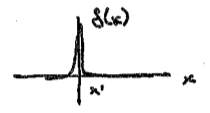
\includegraphics[width=.3\textwidth]{figures/lec10_.png}
    }}
  \ . 
\end{align}
Note that the source is \emph{zero} for everywhere. This means that everywhere to the left of $x=x'$ is described by a homogeneous equation,
\begin{align}
  \mathcal O_x G_<(x,x') = 0 \ .
\end{align}
Further, everything to the right of $x=x'$ is described by \emph{another} homogeneous equation,
\begin{align}
  \mathcal O_x G_>(x,x') = 0 \ .
\end{align}
These are different equations for \emph{different functions}: $G_<$ and $G_>$ are two different functions that obey homogeneous equations \emph{in their respective domains}. $G_<(x,x')$ is \emph{not} defined for $x>x'$. Usually solving homogeneous equations is easier\footnote{I wouldn't really know, but it seems to take less time on \emph{Mathematica} so there you go.}. 

The strategy then  is to solve for $G_<(x,x')$ and $G_>(x,x')$ as functions of $x$ and \emph{patch them together}: 
\begin{align}
  G(x,x') = 
  \begin{cases}
  G_<(x,x') & \text{ if } x<x'\\
  G_>(x,x') & \text{ if } x>x'
  \end{cases}\ .
\end{align}

Here $x'$ is just a spectator variable---we're keeping it fixed. For simplicity, you may even want to shift your coordinates so that $x'=0$. When we do this, we usually have a second order differential equation---some variant of the Laplacian because that's 99\% of what we do---so we need to have enough boundary conditions to fix our cofficients. Since we have two functions in a second order differential equation, we need \emph{four} boundary conditions. When we defined the Green's function problem, presumably we are considering functions over some interval $x,x'\in [a,b]$. This gives boundary conditions at $a$ and $b$, which may even be at $a=-\infty$ and $b=\infty$. The two additional boundaries are obtained at $x=x'$. These come from requiring the continuity of the solutions
\begin{align}
  G_<(x',x') = G_>(x',x')
\end{align}
and a `jump condition' between the first derivatives of the soltuion:
\begin{align}
  \lim_{\epsilon\to 0}\int_{x'-\epsilon}^{x'+\epsilon}dx \mathcal O_x G_(x,x') = 1 \ ,
\end{align}
where this comes from simply integrating the defining equation $\mathcal O_xG(x,x') = \delta(x-x')$ over a sliver around $x=x'$. Since $\mathcal O_x$ is assumed to be second order, the jump condition reduces to saying that the first derivatives of $G_<$ and $G_>$ are discontinuous at $x=x'$ by a certain amount. Applying these boundary conditions then gives a piece-wise solution for the Green's function.


\section{Where we're going}
\label{sec:ways:to:solve:G}

Our primary goal in this course is to find the Green's function $G(x,x')$ given a differential operator $\mathcal O$. There are three primary ways to do this:
\begin{enumerate}
\item \textbf{Eigenfunctions and completeness}, Section~\ref{sec:Greens:fuctions:by:completeness}. Assuming one knows the eigenfunctions of the differential operator, this gives a series solution for the Green's function. It is practically useful only when the series is convergent.

\item \textbf{Patching}, Section~\ref{sec:patching}. This method assume that one can solve the \emph{homogeneous} differential equation $\mathcal O_x G(x,x')=0$ and then produces a piece-wise solution to the \emph{inhomogeneous} differential equation that defines the Green's function, $\mathcal O_x G(x,x')=\delta(x-x')$. This is practically useful in one dimension where the boundary conditions where the pieces are connected are easy to define.

\item \textbf{Fourier transform and its cousins}. This will be the topic of the rest of our course. We convert the differential equation into an \emph{algebraic equation} in momentum space. Aspects of the causal structure of the system that are manifested in complex momentum space. Furthermore, one can use contour integrals to do the `hard work.'
\end{enumerate}

Recently I filled a hole in my undergraduate education and used a fourth method called the \emph{method of variations} to solve inhomogeneous differential equations. The method is sketched out in Appendix~\ref{app:method:of:variations}. We won't have anything further to say about that here, except that it turns out you can get a faculty job in theoretical particle physics without knowing how to use it.

\begin{example}
This problem is from Matthews \& Walker Section 9-4. Consider a unit string with frequency $k= \omega/c$ and Dirichlet boundary conditions at $x=0,1$; where we note that we are using units of `length of the string.' The differential operator describing standing waves is
\begin{align}
  \mathcal O_x = \frac{d^2}{dx^2} + k^2 \ .
 \end{align}
Let's solve this using eigenfunctions. We know the normalized eigenfunctions from Example~\ref{ex:eigenfunction:fourier}:
\begin{align}
  f_n(x) &= \sqrt{2} \sin (n\pi x) 
  &
  \mathcal O_x f_n(x) 
  & = \left(-n^2\pi^2 + k^2\right)f_n(x) \equiv \lambda_n f_n(x) \ .
\end{align}
By the way, it should  have been \emph{obvious} that these are the eigenfunctions and eigenvalues, even though $\mathcal O_x$ is \emph{not} the same as $d^2/dx^2$. Using our completeness relation, the Green's function is
\begin{align}
  G(x,x') &= \sum_n \frac{f^*(x)f(x')}{\lambda_n}
  =
  2\sum_n\frac{\sin(n\pi x) \sin (n\pi x')}{k^2 - n^2\pi^2} \ .
\end{align}
Thus the solution to the system with some inhomogeneous source $s(x)$
\begin{align}
  \left[\frac{d^2}{dx^2} + k^2\right] f(x) &= s(x)
\end{align}
is simply
\begin{align}
  f(x) &= \int_0^1 dx' \, G(x,x') s(x') \ .
\end{align}
\end{example}

\begin{example}\label{ex:patching:eg}
Let's do the same example with the patching method. In this case we start with the equation (the analog of $A(A^{-1}) =\mathbbm{1}$):
\begin{align}
  \left[\frac{d^2}{dx^2} + k^2\right]G(x,x') &= \delta(x-x')
\end{align}
We now separate the domain into $x<x'$ and $x>x'$, with \emph{a priori} independent solutions $G_<(x,x')$ and $G_>(x,x')$:
\begin{center}
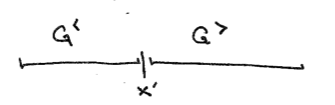
\includegraphics[width=.5\textwidth]{figures/lec11_GgGl.png}
\end{center}
Applying the Dirichlet boundary conditions at $x=0,1$ gives
\begin{align}
  G(x,x') &=
  \begin{cases}
  G_<(x,x') = a\sin(kx) & \text{ for } x < x'\\
  G_>(x,x') = b\sin\left(k(x-1)\right) & \text{ for } x > x'
  \end{cases} \ .
\end{align}
Make sure you understand why $G_>(x,x')$ has a factor of $(x-1)$ and not $x$; this is simply the boundary condition at $x=1$ without setting $b=0$.
The two coefficients $a$ and $b$ must be fixed by the matching at $x=x'$. 
To do this, integrate the second order differential equation over a sliver around $x'$:
\begin{align}
  \int_{x'-\varepsilon}^{x'+\varepsilon}
  dx \, 
  \left[
   \frac{d^2}{dx^2} + k^2
  \right]
  G(x,x')
  &=
  \int_{x'-\varepsilon}^{x'+\varepsilon} dx\, \delta (x-x') \ .
  \label{eq:eg:jump:condition:integration:eg:1}
\end{align}
Note that the $k^2 G$ term in the integrand vanishes since it scales like $\varepsilon$. The integral of the second derivative is simple since it is simply the integral of a derivative, $\int dx\, d/dx(G') = \int d(G') = G'$ so that
\begin{align}
  \left.\frac{d}{dx}G\right|_{x'-\varepsilon}^{x'+\varepsilon}
  &=
  G'_>(x',x') - G'_<(x',x')
  =
   1 \ .
   \label{eq:eg:patching:jump:condition}
\end{align}
This is the jump condition of the first derivative. If we integrate the jump condition once more over a sliver between $x\pm\varepsilon$ gives the continuity condition:
\begin{align}
  G_<(x',x') &= G_>(x',x') \ .
\end{align}
If you are very attentive to details, you may be concerned about doing another integration since \eqref{eq:eg:patching:jump:condition} is simply an equality between numbers. If you are this attentive, I refer to the next example.
The jump and continuity conditions give
\begin{align}
  ka \cos(kx') + 1 &= kb \cos \left(k(x'-1)\right)
  \\
  a\sin(kx') &= b\sin \left(k(x'-1)\right) .
\end{align}
One can solve for the coefficients:
\begin{align}
  a&= \frac{\sin \left(k(x'-1)\right)}{k\sin k}
  &
  b&= \frac{\sin kx'}{k\sin k} \ .
\end{align}
Plugging this all in gives 
\begin{align}
  G(x,x') &=
  \frac{1}{k\sin k}
  \begin{cases}
  \sin kx \, \sin \left(k(x'-1)\right) &\text{ if }x < x'
  \\
  \sin kx' \, \sin \left(k(x-1)\right) &\text{ if }x > x' \ .
  \end{cases}
\end{align}
\end{example}
Observe that you find two \emph{different} expressions for $G$ by these methods. Please confirm---perhaps numerically---that these indeed represent the same function $G(x,x')$. 

\begin{example}%{ex:patching:second:integration}
In the previous example, we integrated the Green's function equation `twice' to get two boundary conditions at $x=x'$. You may be concerned that after doing the first definite integral, we just have a relation between numbers. That is to say, we can no longer `integrate a total derivative' $\int dx\; \partial_x f(x) = f(x)$ because the integrand is not a total derivative, it is just a number. 

It may be helpful to think about this as follows. The first definite integral of the Green's function equation gives the jump condition, \eqref{eq:eg:patching:jump:condition}. For the second integral, we may take
\begin{align}
  \int_{-\varepsilon'}^{\varepsilon'}
  dy \,
  \int_{x'-\varepsilon}^{x'+\varepsilon+y}
  dx \, 
  \left[
   \frac{d^2}{dx^2} + k^2
  \right]
  G(x,x')
  &=
  \int_{-\varepsilon'}^{\varepsilon'}
  dy \,
  \int_{x'-\varepsilon}^{x'+\varepsilon+y}
  dx \, 
  \delta (x-x') 
  \ .
\end{align}
One can compare to \eqref{eq:eg:jump:condition:integration:eg:1}. You should be happy that the right-hand side integrates to zero upon $\varepsilon\, , \, \varepsilon' \to 0$; it is two integrations over an infinitesimal slice with only one $\delta$-function to support it. Following through gives:
\begin{align}
  \int_{-\varepsilon'}^{\varepsilon'}
  dy \,
  \int_{x'-\varepsilon}^{x'+(\varepsilon+y)}
  dx \, 
  \frac{d}{dx}
  \left[
   \frac{d}{dx}
   G(x,x')
  \right]
  &=
  \int_{-\varepsilon'}^{\varepsilon'}
  dy \,
  \left[
   G'(x'+y+\varepsilon,x')
   -
   G'(x'-\varepsilon, x')
  \right] \ .
\end{align}
$G'(x'-\varepsilon, x')$ is simply a constant. Its integral vanishes when we take the limit $\varepsilon\, ,\, \varepsilon'\to 0$. For the first term, we may strategically take $\varepsilon\to 0$  (or otherwise $\varepsilon < \varepsilon'$) so that we now have
\begin{align}
  \int_{-\varepsilon'}^{\varepsilon'}
  dy \,
  \frac{d}{dy}
  \left[
   G(x'+y+\varepsilon,x')
   \right] \ .
\end{align}
Note the subtle sleight of hand: $G'(\cdots, x')$ means ``take the derivative of $G$ with respect to the first argument.'' The variable in the first argument is $y$, so we have written it out explicitly as $d/dy$ so that the $dy$ integral is over a total derivative. This now straightforwardly gives, 
\begin{align}
  G(x'+\varepsilon+\varepsilon', x') 
  -
  G(x'+\varepsilon-\varepsilon', x') 
  = 0 \ ,
\end{align}
which is simply the continuity condition \eqref{eq:eg:patching:jump:condition} once we choose $\varepsilon' > \varepsilon$ with both going to zero.
\end{example}

\begin{exercise}
This example is from Butkov, chapter 12.1. Consider a taut string of length $L$ under the load of a weirdly-shaped rock:
\begin{center}
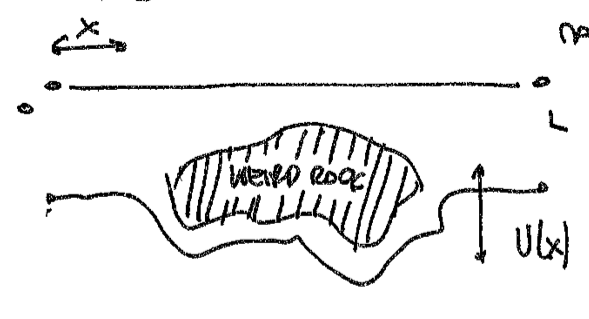
\includegraphics[width=.5\textwidth]{figures/lec12_eg.png}
\end{center}
The force equation for the vertical displacement of the string, $u(x)$, is
\begin{align}
  T u''(x) = F(x),
\end{align}
where $T$ is the tension and $F(x)$ is the force-per-unit-length. One may write this more simply as $u''(x) = f(x) = F(x)/T$. Show that the Green's function may be written as a piecewise function
\begin{align}
  G(x,x') &=
  \begin{cases}
  \left(\frac{x'-L}{L}\right)x  & \text{ if } x<x'
  \\
  \left(\frac{x-L}{L}\right)x' & \text{ if } x>x' 
  \end{cases}\ .
\end{align}
Suppose you replace the weird rock by a square paper weight of size $x < L$ in the middle of the string. Sketch what the paper weight on the string looks like.
\end{exercise}


\section{Example: Stability Analysis (Extra topic)}

% From Numerical Recipes, Ch 20 on PDEs
Suppose we want to solve a partial differential equation numerically.\footnote{This section draws from \emph{Numerical Recipes} by Press et al. The book is a classic but is sometimes overlooked for silly reasons: perhaps it is too old to be relevant for modern computing? Perhaps it is too computational for theorists? Wrong.} We discretize space and time into bins of size $\Delta x$ and $\Delta t$:
\begin{align}
  x_a &= x_0 + a\Delta x & t_n = t_0 + n\Delta t \ .
\end{align}
Suppose we have a simple wave equation for a quantity $u(x,t)$:
\begin{align}
  \partial_t u(x,t)= - v\partial_x u(x,t) \ .
\end{align}
In our discretization, let $u^n_a\equiv u(x_a,t_n)$.
If we choose a space-symmetric spatial derivative, we may write the discretized wave equation as:
\begin{align}
\frac{u^{n+1}_a - u^{n}_a}{\Delta t}
=
-v\left(\frac{u^n_{a+1}-u^n_{a-1}}{2\Delta x}\right) \ .
\end{align}
Suppose we have \emph{initial data} about the configuration, $u(t_0, x)$ for all $x$. The discretization gives a way to numerically calculate the configuration over all $x$ at the next slice in $t$:
\begin{align}
  u_a^{n+1} = u^n_a 
  + \Delta t
  \left[-v\left(\frac{u^n_{a+1}-u^n_{a-1}}{2\Delta x}\right)\right] \ .
  \label{eq:FTCS}
\end{align}
This is called the Euler algorithm, or more precisely a \emph{forward time centered space} representation. This is clearly a numerical approximation to a continuous equation. A good question is: how good of an approximation is it?

There's a method call the Von Neumann stability analysis that uses Fourier series to answer this question. This analysis was invented by Clark and Nicolson rather than the physicist and computer scientist John von Neumann after whom it is named.\footnote{This is Stigler's law of eponymy. Stigler himself explains that he was not the first to present the idea.} The idea is to write $u^n_a$ as a Fourier series over plane waves with momentum (wave number) $k$:
\begin{align}
  u^n_a \sim  e^{ika\Delta x} \ .
\end{align}
Plugging this into \eqref{eq:FTCS} gives
\begin{align}
  u^{n+1}_a = 
  \left[1 - i v\frac{\Delta t}{\Delta x}\sin k\Delta x\right]u^n_a \ ,
\end{align}
where we identify the bracketed term as a $k$-dependent prefactor $c(k)$:
\begin{align}
   c(k) = 1 - i v\frac{\Delta t}{\Delta x}\sin k\Delta x \ .
\end{align}
The time evolution of a given $k$ mode is simply a power of $c(k)$:
\begin{align}
  u^{n}_a &= c(k)^n e^{ika\Delta x} \ .
\end{align}
Our expression for $c(k)$ is a complex number with modulus strictly greater than 1 for all $k$. That means that the prefactor of \emph{any} mode diverges. The numerical integration scheme is intrinsically unstable. This is often expressed as the statement: never use Euler forward differencing when numerically solving a differential equation.

Our analysis was strictly for the wave equation: a first order partial differential equation with constant coefficients. A more sophisticated partial differential equation has coefficients that may depend on space and time. The Von Neumann analysis is valid as long as the coefficients vary slowly relative to our discretization.

\begin{exercise}
There are simple tweaks to our integration method that can cure the forward differencing instability. One method is called the Lax method. The proposal is to write the time derivative in a funny way:
\begin{align}
  \partial_t u(t_n, x_a) \to
  \frac{
    u^{n+1}_a 
    - \frac{1}{2}\left(u^n_{a-1}+u^n_{a+1}\right)
    }{ \Delta t } \ .
\end{align}
Show that this modifies the Von Neumann analysis to give a coefficient
\begin{align}
  c(k) = \cos k\Delta x - i v\frac{\Delta t}{\Delta x}\sin k\Delta x \ ,
\end{align}
so that the stability condition is
\begin{align}
\frac{\Delta t}{\Delta x} \leq |v| \ .
\end{align}
This condition is called the Courant condition and is fairly generic for numerical solutions to first-order differential equations.
\end{exercise}


% Not eigenmodes if the PDE is more complex, but if we assume the coefficients very slowly relative to the discretization it is a good approx



\part{Complex Analysis}

\chapter{Why complex analysis?}

\section{Why are we doing this?}

We now switch gears to complex analysis. One of the results that I hope you'll come to appreciate in your study of physics is the rich role of complex numbers (and their generalizations) in describing nature. Our study of complex analysis will focus on motivating the residue theorem to calculate integrals in complex space. This, in turn, is useful when we represent functions in \emph{momentum space} by Fourier transforming. For example, a Green's function $G(x,x')$ can be written with respect to the Fourier momentum variable $k$ by
\begin{align}
  G(x,x') &= \int \dbar k \, e^{-ikx} \tilde G(k,x') \ ,
  \label{eq:complex:intro:G:fourier}
\end{align}
where I've used a convenient notation where $\dbar = d/2\pi$. This, in turn is useful because our defining relation for the Green's function is \eqref{eq:Greens:func:as:inverse}:
\begin{align}
  \mathcal O_xG(x,x') &= \delta(x-x') \ ,
\end{align}
which we may then write (Fourier transforming both sides) as
\begin{align}
  \mathcal O_x \int \dbar k \, e^{-ikx} \tilde G(k,x') 
  =
  \int \dbar k \, e^{-ikx} e^{ikx'} \ .
  \label{eq:complex:intro:defining:G:}
\end{align}
On the right-hand side we've written the $\delta(x-x')$ in its Fourier representation. We have assumed that $\mathcal O_x$ is a polynomial in derivatives with respect to $x$:
\begin{align}
  \mathcal O_x = \sum_{n=0}^{\infty}
  p_n(x) \left(\frac{d}{dx}\right)^n
  \equiv P\left(x,\frac{d}{dx}\right) \ .
  \label{eq:complex:intro:defining:Ox}
\end{align}
What's powerful about this is that that when we apply a differential operator in $x$ onto the Fourier representation of a function, say \eqref{eq:complex:intro:G:fourier}, then the derivatives only `see' the exponential factor $e^{-ikx}$. This means that derivatives are particularly easy:
\begin{align}
  \left(\frac{d}{dx}\right)^n e^{-ikx} &= (-ik)^n \ .
\end{align}
This means that we may write the differential operator $\mathcal O_x$ in \eqref{eq:complex:intro:defining:Ox} when it acts on the Fourier basis function $e_{(k)}(x) = e^{-ikx}$ as
\begin{align}
  \mathcal O_x e^{-ikx} = \sum_{n=0}^{\infty}
  p_n \left(-ik\right)^n e^{-ikx}
  \equiv P(-ik) e^{-ikx}  \ .
\end{align}
For simplicity we have assumed that the polynomial coefficients in $x$ are simply constants, $p_n(x) = p_n$, and written $P(y) \equiv P(0,y)$.\footnote{This simplification does not affect anything in this course. For the more general case, one would want to also Fourier transform the $p_n(x)$ and use the convolution theorem to write everything as a single Fourier expansion; see e.g.~\url{https://mathoverflow.net/a/37873}.}
The defining relation for $G$,
\eqref{eq:complex:intro:defining:G:}, may in turn be simplified:
\begin{align}
  \int \dbar k \, e^{-ikx} P(-ik) \tilde G(k,x') &= \int \dbar k \, e^{-ik(x-x')} \ ,
\end{align}
which suggests a simple expression for the Fourier coefficients:
\begin{align}
  \tilde G(k,x') &= e^{ikx'} \left[P(-ik)\right]^{-1} \ ,
  \label{eq:Greens:function:Fourier:transform:heuristic}
\end{align}
where one may find $G(x,x')$ from simply taking the inverse Fourier transform. There will turn out to be a few neat features of this approach, but before getting there, let's start from the very beginning.

\begin{exercise}
This procedure is completely analogous to solving $A \vec{g} = \mathbbm{1}$ for $\vec{g}$ by expanding in eigenfunctions of $A$, $\vec g = g^k \vec{e}_{(k)}$. Then we have $A\vec{g} = \sum_k \lambda_k g^k e_{(k)}$. Follow through this analogy to argue that \eqref{eq:Greens:function:Fourier:transform:heuristic} corresponds to $g^k = c_k/\lambda_k$ where $c_k$ is identified with $e^{ikx'}$.
\end{exercise}

\begin{exercise}
For $\mathcal O_x = (d/dx)^2$, what is the value of $P(-ik)$? What is $\tilde G(k,x')$?
\end{exercise}

\section{Complex Numbers}


A complex number $z$ may be decomposed into real and imaginary parts
\begin{align}
  z = x + i y \ ,
\end{align}
where $x$ and $y$ are both real numbers. We may also define the complex conjugate as
\begin{align}
  \bar z = z^* = x - i y \ .
\end{align}
One may also write these variables in a polar notation,
\begin{align}
  z &= re^{i\theta}
  &
  \bar z &= re^{-i\theta} \ ,
\end{align}
where $r \in [0,\infty]$ and $\theta \in [0, 2\pi]$:
\begin{center}
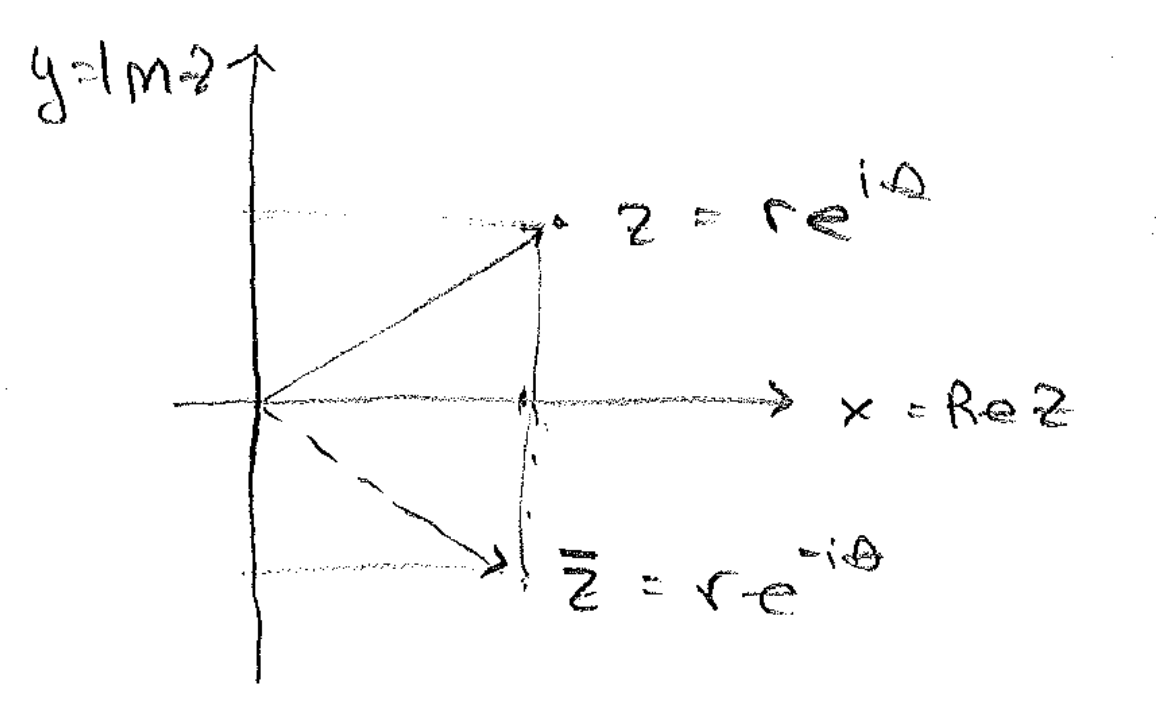
\includegraphics[width=.5\textwidth]{lec13_complexvar}
\end{center}
Complex numbers live in the space of complex numbers $\mathbbm{C}$, a \emph{two-dimensional} real space with coordinates $(x,y)$ in $\mathbbm{R}^2$ augmented by an additional rule for multiplication (take two complex numbers and return a complex number) that is called the \emph{complex structure}. This is basically the definition $i^2 = -1$, though one may generalize to higher complex dimensions. 

\section{Complex functions}

Complex functions take complex numbers and return complex numbers. Inspired by the two-dimensional-ness of $\mathbbm{C}$, let us write a complex function as $f(z)=f(x,y)$ where $z = x+i y$. Because $f(x,y)$ is, itself, a complex number for a given $z=x+i y$, we can decompose $f$ into two real-valued functions
\begin{align}
  f(z) = f(x,y) &= u(x,y) + i v(x,y) \ .
\end{align}
This is clearly a map from $\mathbbm{C} \to \mathbbm{C}$ and so we can simply ``do multivariable calculus'' on this space. 

\begin{exercise}
The goal of this problem is to review line integrals in a 2D space. Perform the integral
\begin{align}
  \int_i^{1+i} dz \; z \,
\end{align}
with respect to the path that connects $z=i$ and $z=i+1$ by a straight line segment. This is \emph{not} a closed loop, there's no magic formula for this. Just parameterize the path by writing $z$ as a function of a real parameter. Then write out $dz$ in terms of the parameter. Do the integral. Answer: $\frac{1}{2}+i$.

 Integrals on the complex plane can seem mysterious because we end up using tricks that we develop below. This problem is to remind you that what we are doing is really a version of the Riemann sum with complex-valued chunks. 
\end{exercise}

The ``trick'' here is that we have interpreted the complex integral of a complex function over a complex variable as an integral over a \emph{real} variable, the path parameter. This is now a real integral over a function that happens to have factors that contain some funny constant $i$.  Here is a more telling example. 
\begin{exercise}
Let us integrate the function
\begin{align}
  f(z) = \frac{1}{z}
\end{align}
over two paths from $z=-1$ to $z=+1$. These paths correspond to the upper and lower half-circles around the origin, $z(t)= e^{i\pi t} $ over $t\in[1,0]$ and over $t\in[1,2]$. In each case the measure is $dz = i\pi z \, dt$. Show that the results for these two paths are
\begin{align}
  \int_1^0 \frac{dz}{z} &= -i\pi t 
  &
  \int_1^2 \frac{dz}{z} &= i\pi t  \ .
\end{align}
\end{exercise}
The previous example emphasizes two key points:
\begin{enumerate}
  \item To fully define a complex integral, one must define the integration path. In general, different integration paths give different answers. 
  \item The answer is not the same as the one you would get from doing a \emph{real} indefinite integral $\int dx\, x$ and then evaluating the result for complex values.
\end{enumerate}

If we forget the complex structure, then this \emph{seems} to simply be the calculus of maps between $\mathbbm{R}^2 \to \mathbbm{R}^2$ where
\begin{align}
  f(x,y) &= u(x,y) \hat{\vec{x}} + v(x,y)\hat{\vec{y}} \ .
\end{align}
In that case, we need to collect the partial derivatives. On the one hand, we may write the differential of $f$ as
\begin{align}
  df = \frac{\partial f}{\partial x} dx + \frac{\partial f}{\partial y} dy \ .
\end{align}
Please note that the partial derivatives of $f$ contain both real and imaginary parts. That is to say: $\partial f/\partial x$ generally contains both real ($\hat x$) and imaginary ($\hat y$) pieces. 

% From Appel, Ch. 4.1.c
From the definitions of $z=x+iy$ and $\bar z = x-iy$, we may write $dz = dx+idy$ and $d\bar z = dx-idy$. This lets us rewrite
\begin{align}
  dx &= \frac{1}{2}(dz+d\bar z)
  &
  dy &= \frac{1}{2i}(dz-d\bar z) \ .
\end{align}
Plugging this into our expression for the differential of $f$ gives
\begin{align}
  df &= \frac{1}{2}
  \left(
    \frac{\partial f}{\partial x}
    -i\frac{\partial f}{\partial y}
  \right)dz
  + 
  \frac{1}{2}
  \left(
    \frac{\partial f}{\partial x}
    +i\frac{\partial f}{\partial y}
  \right)d\bar z 
  \\
  &\equiv \frac{\partial f}{\partial z}dz
  + \frac{\partial f}{\partial \bar z}d\bar z
  \label{eq:complex:2D:deviation}
  \ .
\end{align}
From this we may identify the partial derivatives in the $z$ and $\bar z$ coordinates:
\begin{align}
  \frac{\partial}{\partial z} &= 
  \frac{1}{2}
  \left(
  \frac{\partial}{\partial x}
  -i
  \frac{\partial}{\partial y}
  \right)
  &
  \frac{\partial}{\partial \bar z} &= 
  \frac{1}{2}
  \left(
  \frac{\partial}{\partial x}
  +i
  \frac{\partial}{\partial y}
  \right) 
  \ .
  \label{eq:ddz:ddzst}
\end{align}
The fact that partial derivatives combine like this may be familiar\footnote{This comes from the underlying mathematical structure. The partial derivatives are basis vectors for the \emph{tangent space} at some point $(x,y)$. These partial derivatives ask: how much does the function I'm acting on change if I move by one unit in this direction?}. 

So far we have emphasized that $f(x,y)$ behaves like a function in two real dimensions. Critically, in some ways we want to think about functions $f(z)$ that are functions of `one' [complex] dimension rather than two real dimensions. In two real dimensions, calculus came with a notion of directional derivative. When we wanted the rate of change for a function, we had to ask \emph{in what direction} are we checking the rate of change. At a given function may change by a positive amount in the $x$-direction, but a negative amount in the $y$-direction, for example. This is in contrast to one-dimensional calculus where each point had an unambiguous derivative that represented how much the function changed in the positive $x$ direction with respect to a point $x_0$:
\begin{align}
  df(x) = \frac{d f(x_0)}{d x} (x-x_0) + \cdots \ .
\end{align}
This is in contrast to the change in a general complex function \eqref{eq:complex:2D:deviation}. In fact, if we explicitly wrote some expansion with respect to a point $z_0$, it looks a little funny:
\begin{align}
  df(z) &= 
  \frac{\partial f}{\partial z}(z-z_0) +
  \frac{\partial f}{\partial \bar z}(\bar z-\bar z_0) + \cdots \ .
\end{align}
What is going on here? Why should $f(z)$ be a function of one complex variable $z$ but the expansion seems to depend not only on $(z-z_0)$ but also $(z-z_0)^*$? 




\section{Analytic complex functions are nice}

This leads us to a definition of ``nice'' complex functions. The following terms are all more-or-less equivalent for this sense of nice-ness: \textbf{[complex] differentiable}, \textbf{analytic}, \textbf{holomorphic}, \textbf{regular}. This is simply the restriction that the $\partial f/\partial \bar z$ term should vanish so that the variation $f(z)$ only depends on $\delta z$ and not $\delta\bar z$. In other words, an analytic function admits usual single-dimensional definition of the derivative,
\begin{align}
  \frac{df(z_0)}{dz} &= \lim_{z\to z_0} \frac{f(z)-f(z_0)}{z-z_0} \ .
  \label{eq:df:dz:analytic:def}
\end{align}
The key aspect of this is that there is only \emph{one} value of $df/dz$ at $z_0$ no matter how you approach $z_0$. In other words, it doesn't matter if $\delta z = z-z_0$ is coming from the positive/negative real/imaginary direction. The value of $df/dz$ is the same. 

\begin{example}
We cannot overemphasize the interpretation of analyticity here. The left-hand side of \eqref{eq:df:dz:analytic:def} is supposed to be a \emph{unique number}, analogous to the slope of $f$ at $z_0$. However, on the right-hand side you can see that the denominator is very different if we take $z = z_0+ i \epsilon$ or $z= z_0 + \epsilon$ for real $\epsilon$. In the first case the denominator gives an overall factor of $-i = i^{-1}$ to $df(z_)/dz$, in the second case it does not. Thus the idea of having a unique `slope' at $z_0$ hinges on requiring $f(z)$ to be sufficiently well-behaved that it does not matter how $z$ approaches $z_0$.
\end{example}

For most of these lectures we will use the term \textbf{analytic} to refer this property. Let us see what happens when we impose $df/d\bar{z} = 0$ onto the component functions $u(x,y)$ and $v(x,y)$:
\begin{align}
  \frac{1}{2}\left(\frac{\partial}{\partial x} + i \frac{\partial}{\partial y}\right)
  \left[u(x,y)+iv(v,y)\right]
  &= 
  \frac{1}{2}
  \left( \frac{\partial u}{\partial x} - \frac{\partial v}{\partial y} \right)
  +
  \frac{i}{2}
  \left( \frac{\partial u}{\partial y} + \frac{\partial v}{\partial x} \right)
  = 0 \ .
\end{align}
This implies the \textbf{Cauchy--Riemann equations}, which are equivalent to the function $f$ being analytic:
\begin{align}
  \frac{\partial u}{\partial x} & = +\frac{\partial v}{\partial y}
  &
  \frac{\partial u}{\partial y} & = -\frac{\partial v}{\partial x} \ .
\end{align}

Thus far we've talked about functions being analytic or not. It turns out that analytic functions are \emph{so} nice that there really aren't that many physically relevant functions that are analytic \emph{everywhere}\footnote{The analog here is people who are nice. Most people are nice most of the time. But very few people are nice \emph{all} of the time. I suspect Fred Rogers may be one of the few who could plausibly be \sout{analytic} \emph{nice} everywhere.}. Instead, we will often talk about functions that are analytic in most places but are not analytic (differentiable) in other places. Indeed, the \emph{non}-analyticity of Green's functions is a key result in this class.


\section{Analyticity is Differentiability}

We have motivated the Cauchy--Riemann equations from the notion of being independent of $\bar z$. This is a useful crutch and fits our theme of motivating rather than rigorously proving results. Let us be clear, however, that the underlying definition of analyticity is that:
\begin{quote}
a function that is analytic at a point $z_0$ is differentiable at $z_0$.
\end{quote}
A function is differentiable at a point $z_0$ if its derivative, \eqref{eq:df:dz:analytic:def}, has a well-defined \emph{finite} value. A function that is itself infinite at a point cannot have a well-defined limit \eqref{eq:df:dz:analytic:def}, and thus are \emph{not} analytic at that point.
We distinguish this from $df/d\bar z =0$ because of the importance of \emph{singular} functions in physics. 
\begin{example}
The following function is non-analytic at $z=2i$ and $z=1$:
\begin{align}
  f(z) = \frac{3z}{(z-2i)(z-1)} \ .
\end{align}
It may seem like $df/dz^* = 0$ at these points because $f(z)$ is independent of $\bar z$. However, one cannot say that $df/\bar dz=0$ because the limit definition analogous to \eqref{eq:df:dz:analytic:def} is not defined. 
\end{example}
\begin{exercise}
The notion of `independent of $\bar z$' sometimes causes more confusion than its worth. After all, $z$ and $\bar z$ are clearly \emph{not} independent variables. Given $z$, you know exactly what $\bar z$ is. The notion in which we \emph{pretend} that $z$ and $\bar z$ are independent is that
\begin{align}
  \frac{\partial z}{\partial \bar z} = 
  \frac{\partial \bar z}{\partial z} = 0 \ ,
\end{align}
which we understand to come from an interpretation of $\mathbbm C \sim \mathbbm R^2$. Use \eqref{eq:ddz:ddzst} to prove the above partial derivative relations.
\end{exercise}

\section{A geometric point of view}
\label{sec:analytic:geometric}

For culture, let us comment on a geometric perspective of analyticity/complex-differentiability. The differential of a function, $df$, is a \textbf{differential one-form}. If you recall some of our nomenclature for dual vectors, a one-form is a kind of `row vector': it is a linear function that takes in a vector and spits out a number.\footnote{The number that is spit out is unique for each spacetime point $z_0$, but is independent of which direction on the complex plane one is probing the `slope' of the function $f$.} If $df$ is such a dual vector, what is the vector space upon which it acts?

\subsection{Geometry}

Consider the differential of $f$ at a specific point $z_0$ in the complex plane: $df(z_0)$. This is not a number---it is a dual vector. In order to get a number from this, you have to feed it a vector. What are the vectors? A vector is an element of the tangent plane\footnote{The tangent plane is exactly what it sounds like: if you have a curved surface like a globe, the tangent plane at $z_0$ and glued a rigid piece of cardboard to one point, $z_0$. Now imagine that the piece of paper has graph paper on it.} of the complex plane at $z_0$: $T_{z_0}\mathbbm{C}$. We can sketch this if you allow me to artificially `curve' the complex plane to help make it easy to distinguish:
\begin{center}
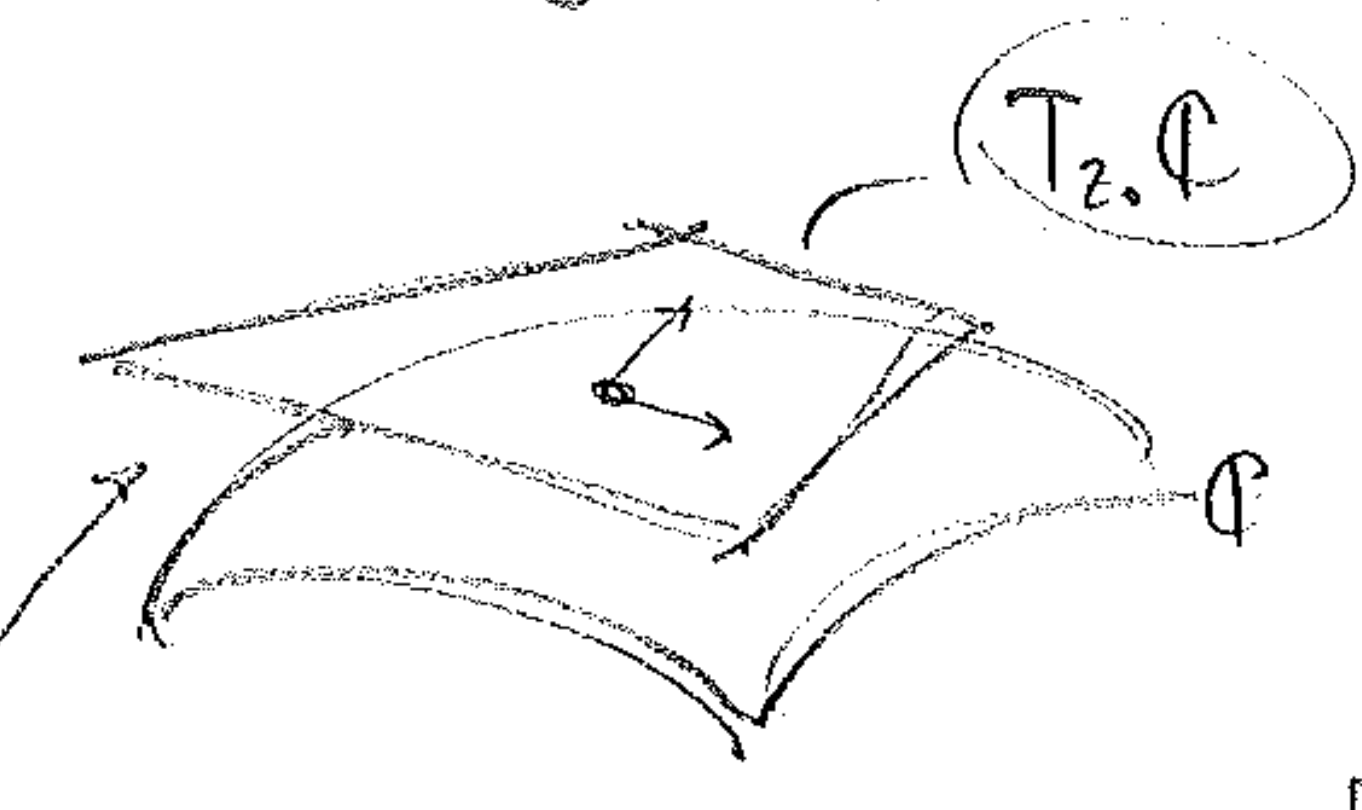
\includegraphics[width=.5\textwidth]{figures/lec13_mani.png}
\end{center}
Using the jargon of differential geometry, we call the complex plane the \emph{base manifold}. The set of all tangent spaces is called a \emph{tangent bundle}\footnote{More general types of vector spaces can be attached to each point of the base manifold. These are called fiber bundles. They are the underlying mathematical structure of mechanics and reflect why Hamilton's equations are so damn special. They are also the mathematical structure that defines gauge theories and so address the question ``what is a force?''}. Each tangent space is a vector space attached to a single point of the base space. 

The object $df(z_0)$ is a dual vector on the vector space\footnote{The standard notation is to write a dual vector of a space $V$ as a vector in the dual space $V^*$, so one could write $df(z_0) \in T^*_{z_0}(\mathbbm{C})$.} $T_{z_0}(\mathbbm{C})$.  The vectors of this space are `velocities' of trajectories that pass through $z_0$. For now let's think of them as quantities
\begin{align}
  \vec v = v^1 + i v^2 = \Delta x + i \Delta y \ .
\end{align}
where we identify $v^1 = \Delta x$ and $v^2 = \Delta y$. Alternatively, $\vec{v}$ can be thought of as a `velocity' along some trajectory $\gamma(t)$ on the space $\mathbbm{C}$. The velocity in the real direction is $v^1 = d\gamma^1(t)/dt$ and the velocity in the imaginary direction is $v^2 = d\gamma^2(t)/dt$, where $\gamma = \gamma^1 + i \gamma^2$.\footnote{This is a vector space with $\vec{e}_{1} = 1$ and  $\vec{e}_{2} = 2$. The only difference from $\mathbbm{R}^2$ is that the vector space $\mathbbm{C}$ is equipped with a complex structure: the rule $i^2 = -1$.}

\begin{center}
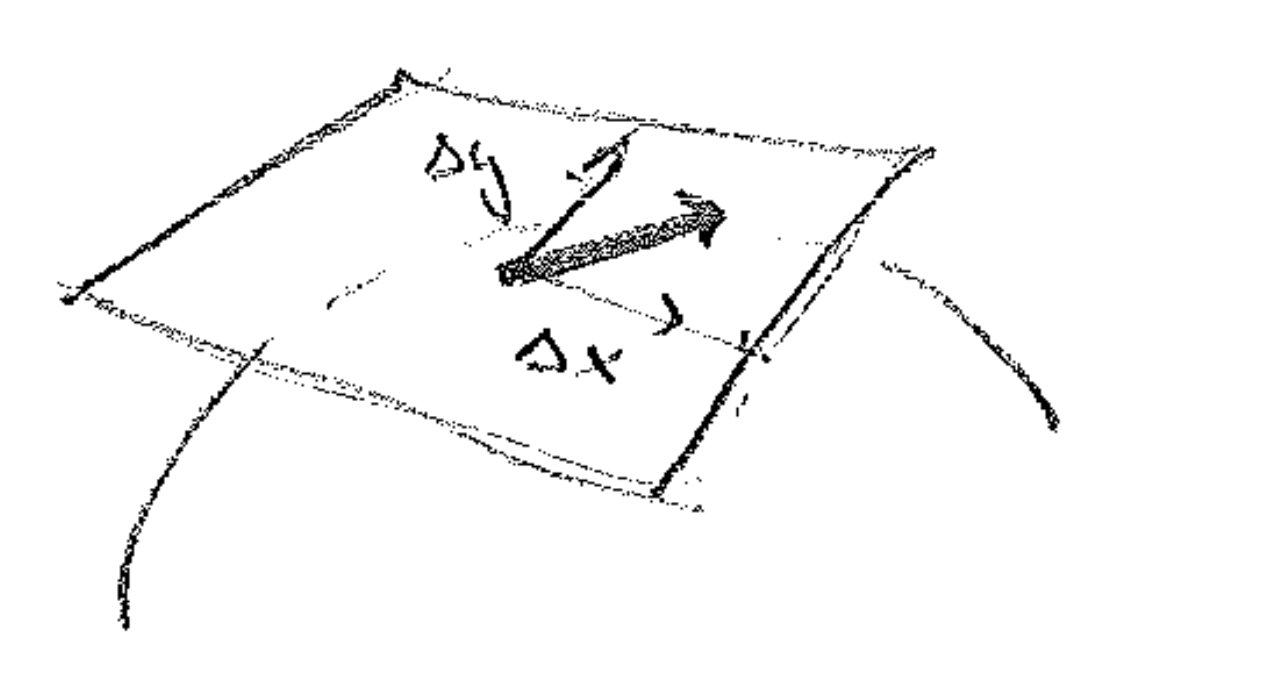
\includegraphics[width=.5\textwidth]{figures/lec13_tanvec.png}
\end{center}
Then we may write the linear action of $df(z_0)$ on $\vec v \in T_{z_0}(\mathbbm{C})$ as
\begin{align}
  df(z_0)\left[\vec{v}\right] &=
  f'(z_0)\left(v^1 + i v^2\right)
  % \Delta x + f'(z_0)i\Delta y 
  \ ,
  \label{eq:diff:geo:CR:1}
\end{align}
where we assume that $f$ is analytic so that $f'(z_0)$ is unambiguously defined (independent of the direction of $\delta z$) as in \eqref{eq:df:dz:analytic:def}. 

However, if we think about this complex space as a two-dimensional real space, the following is also true:
\begin{align}
  df(z_0)\left[\vec{v}\right] &=
  \left.\frac{\partial f}{\partial x}\right|_{z_0} \Delta x
  +
  \left.\frac{\partial f}{\partial y}\right|_{z_0} \Delta y
  =
  \left.\frac{\partial f}{\partial x}\right|_{z_0} v^1
  +
  \left.\frac{\partial f}{\partial y}\right|_{z_0} v^2
  \label{eq:diff:geo:CR:2}
\end{align}
Comparing \eqref{eq:diff:geo:CR:1} and \eqref{eq:diff:geo:CR:2} gives 
\begin{align}
  \frac{\partial f}{\partial x} = f'(z_0) = - i\frac{\partial f}{\partial y} \ .
\end{align}
Recalling that $f= u+iv$ then gives
\begin{align}
  \frac{\partial u}{\partial x}
  + i
  \frac{\partial v}{\partial x}
  =
  -i
  \frac{\partial u}{\partial y}
  +
  \frac{\partial v}{\partial y} \ .
\end{align}
Setting the real and imaginary parts equal to one another give, as expected, the Cauchy--Riemann equations. 

\subsection{Linear Algebra}

The geometric discussion may seem a bit too slick; after all, comparing $\mathbbm{C}$ to $\mathbbm{R}^2$ can be a little subtle.  The key idea is that that $df(z_0)$ should be `single valued' and independent of the direction $\vec{v}$. This is an idea that we have already met in linear algebra. Review our discussion in Section~\eqref{sec:d:as:one:form} regarding the differential of a function. 

The differential $df$ is a member of the cotangent bundle. The specific member $df(z_0)$ is a member of the cotangent space of the base space $\mathbbm{C}$ at the point $z_0$. This is a covector that eats vectors from the tangent space at $z_0$, $T_{z_0}\mathbbm{C}$. Like any covector/row vector/one form, it is a linear function that takes in any vector and spits out a number. The coordinates of the covector are completely independent of the vector that you feed it. This is an \emph{obvious} statement about linear functions. The most basic example is $f(x)=ax$ is completely specified by the coordinate $a$ and is a linear function that takes in any $x$ and spits out a number $ax$. 

Thus the notion that $df(z_0)$ should be a constant---that is, it should be independent of the vector that it eats---is simply the statement that it is a one-form and is thus a linear function from $T_{z_0}\mathbbm{C}$ to numbers.

\section{Analytic and harmonic (optional)}

One more comment is in order. If a function $f(z) = u(x,y)+ i v(x,y)$ is analytic, then its real and imaginary parts are independently 2D harmonic with respect to $\mathbbm{R}^2$:
\begin{align}
  \partial_x^2 u(x,y) + \partial_y^2 u(x,y) &= 0
  &
  \partial_x^2 v(x,y) + \partial_y^2 v(x,y) &= 0 \ .
\end{align}
Harmonic functions show up all over the place---though admittedly you probably care mostly about three-dimensional harmonic functions. The above realization may be helpful, however, for 3D systems for which the third dimension is trivial. For example, you may want to consider fluid flow across an airplane wing. One can take the limit where the wing is infinitely long so that the fluid dynamics reduces to the two-dimensional motion around a cross section of the wing. Alternatively, maybe you care about an electrostatic system which are similarly `effectively' 2D. In this case you can `promote' your real harmonic variable (a fluid dynamics potential or electrostatic potential) to an analytic function and then bear the full power of complex analysis to attack the problem. One of the most fascinating---if outdated---methods is called \textbf{conformal mapping} by which one can solve for a harmonic function with weird boundary conditions by mapping to much simpler boundary conditions. This topic is beautiful and gives a first, intuitive example of \emph{conformal transformations} which are a pillar of theoretical physics (in any discipline). The technique is how engineers in the pre-personal computer era designed airplane wings. For experimentalists, it is pretty neat that \acro{UCR}'s own Nathan Gabor has created an analogous micromagnetic `solver' of this very same problem\footnote{\url{https://arxiv.org/abs/2002.07902}}.


\section{Complex functions as maps}

A complex function $f(z)$ takes in a complex number and returns a complex number. These are maps of the complex plane to itself. It is useful to build an intuition for this rather trivial-sounding statement: complex functions `deform' the complex plane. 

\begin{example}
Consider the function that multiplies a complex number by a constant phase,
\begin{align}
  f(z) = e^{i\theta} z \ .
\end{align}
This takes each point and rotates it in the counterclockwise direction by $\theta$. 
\begin{center}
% 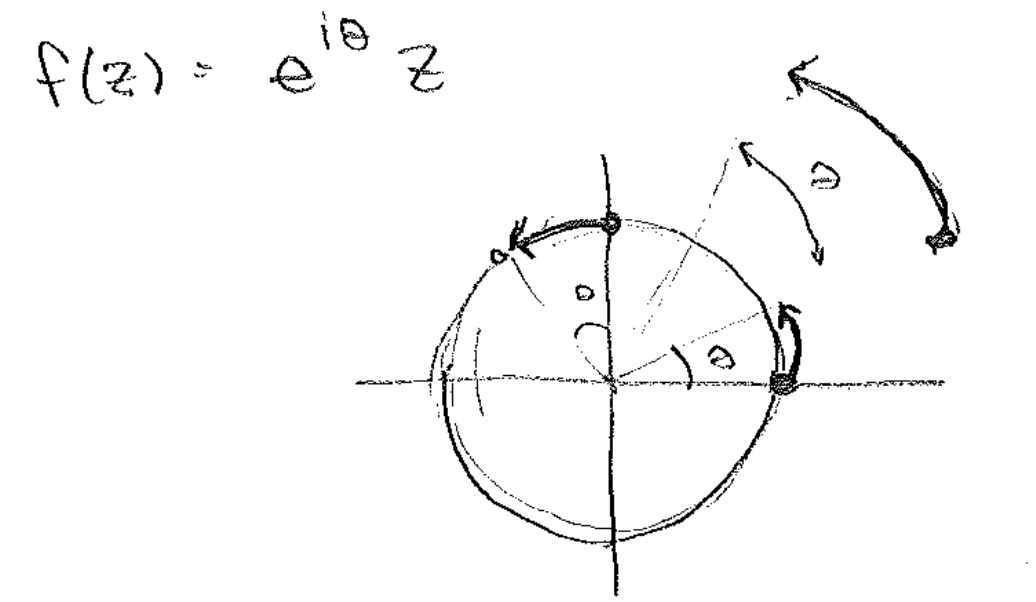
\includegraphics[width=.5\textwidth]{figures/lec13_map1.png}
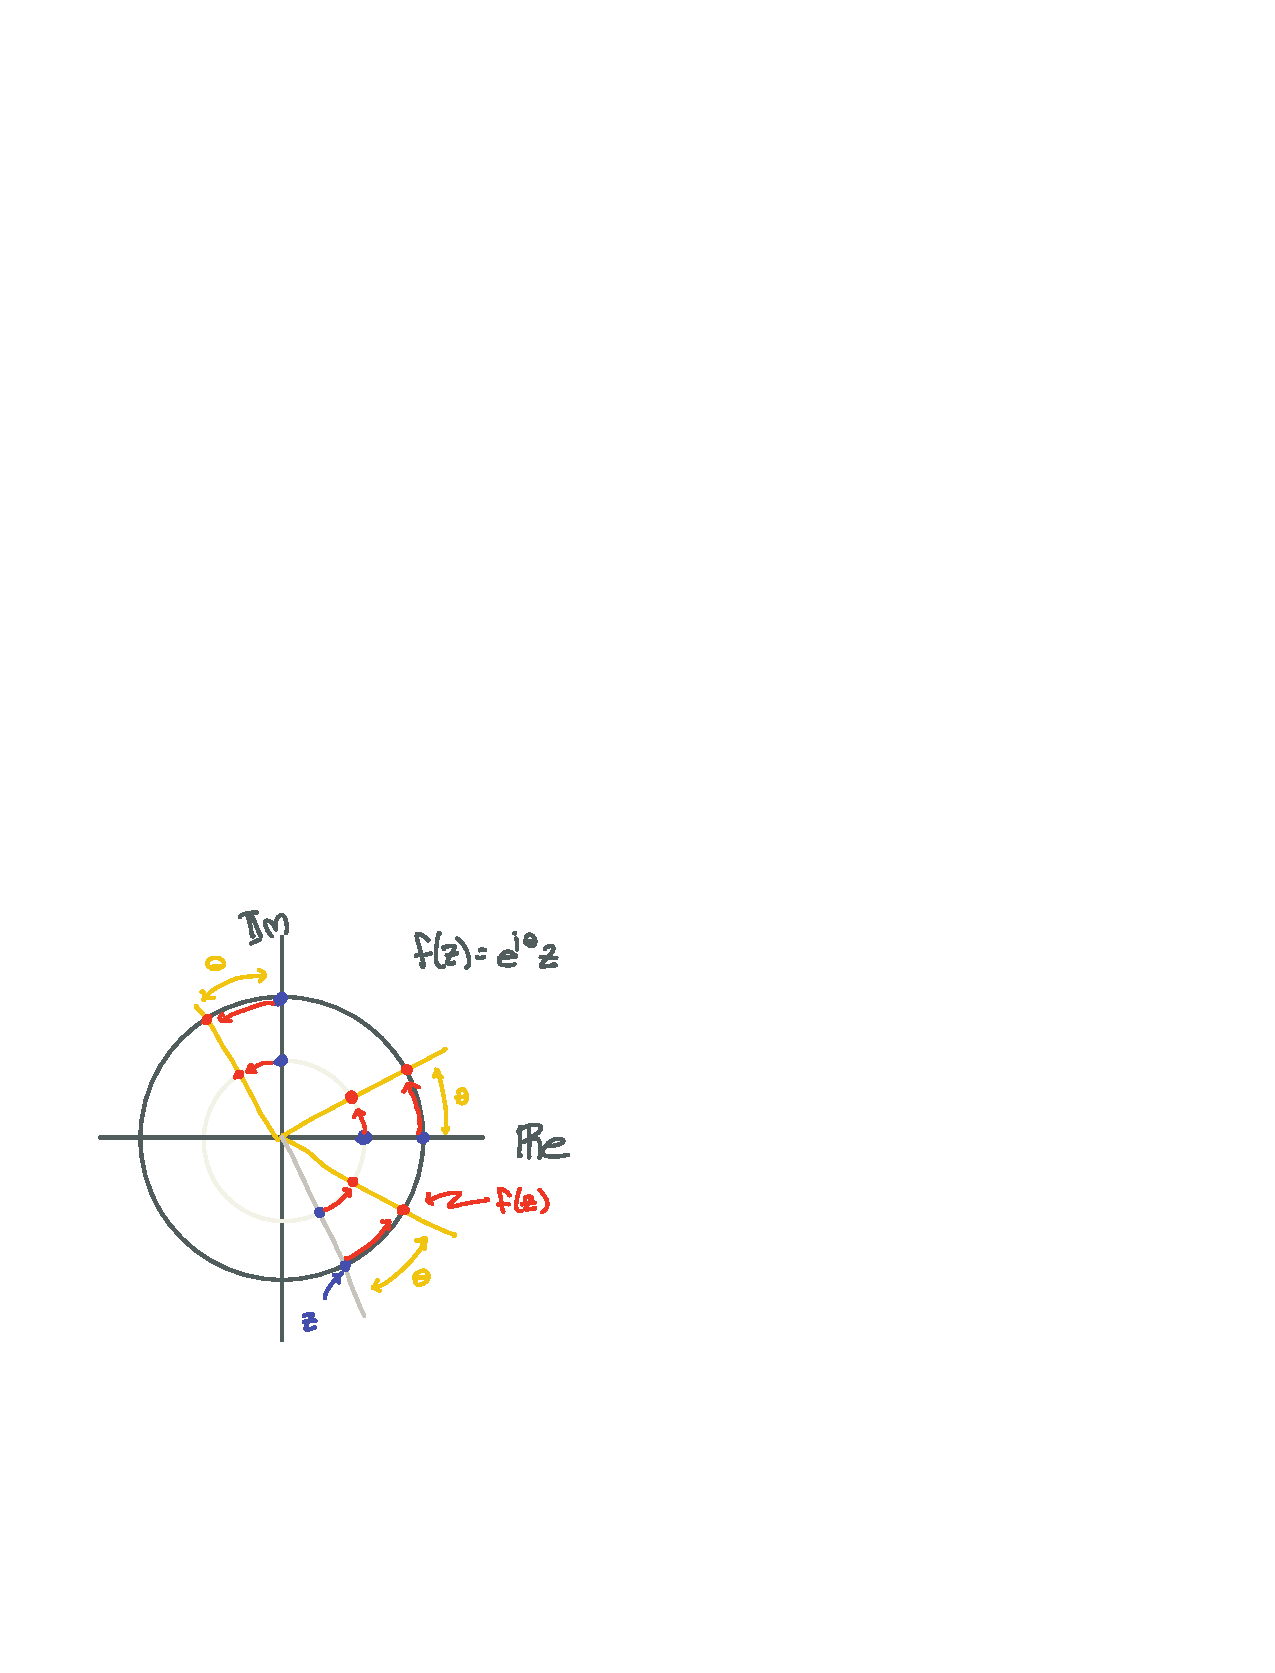
\includegraphics[width=.4\textwidth]{figures/Complex_01_rot.pdf}
\end{center}
\end{example}
We can see this more viscerally by imagining the action on the image of a cat:
\begin{center}
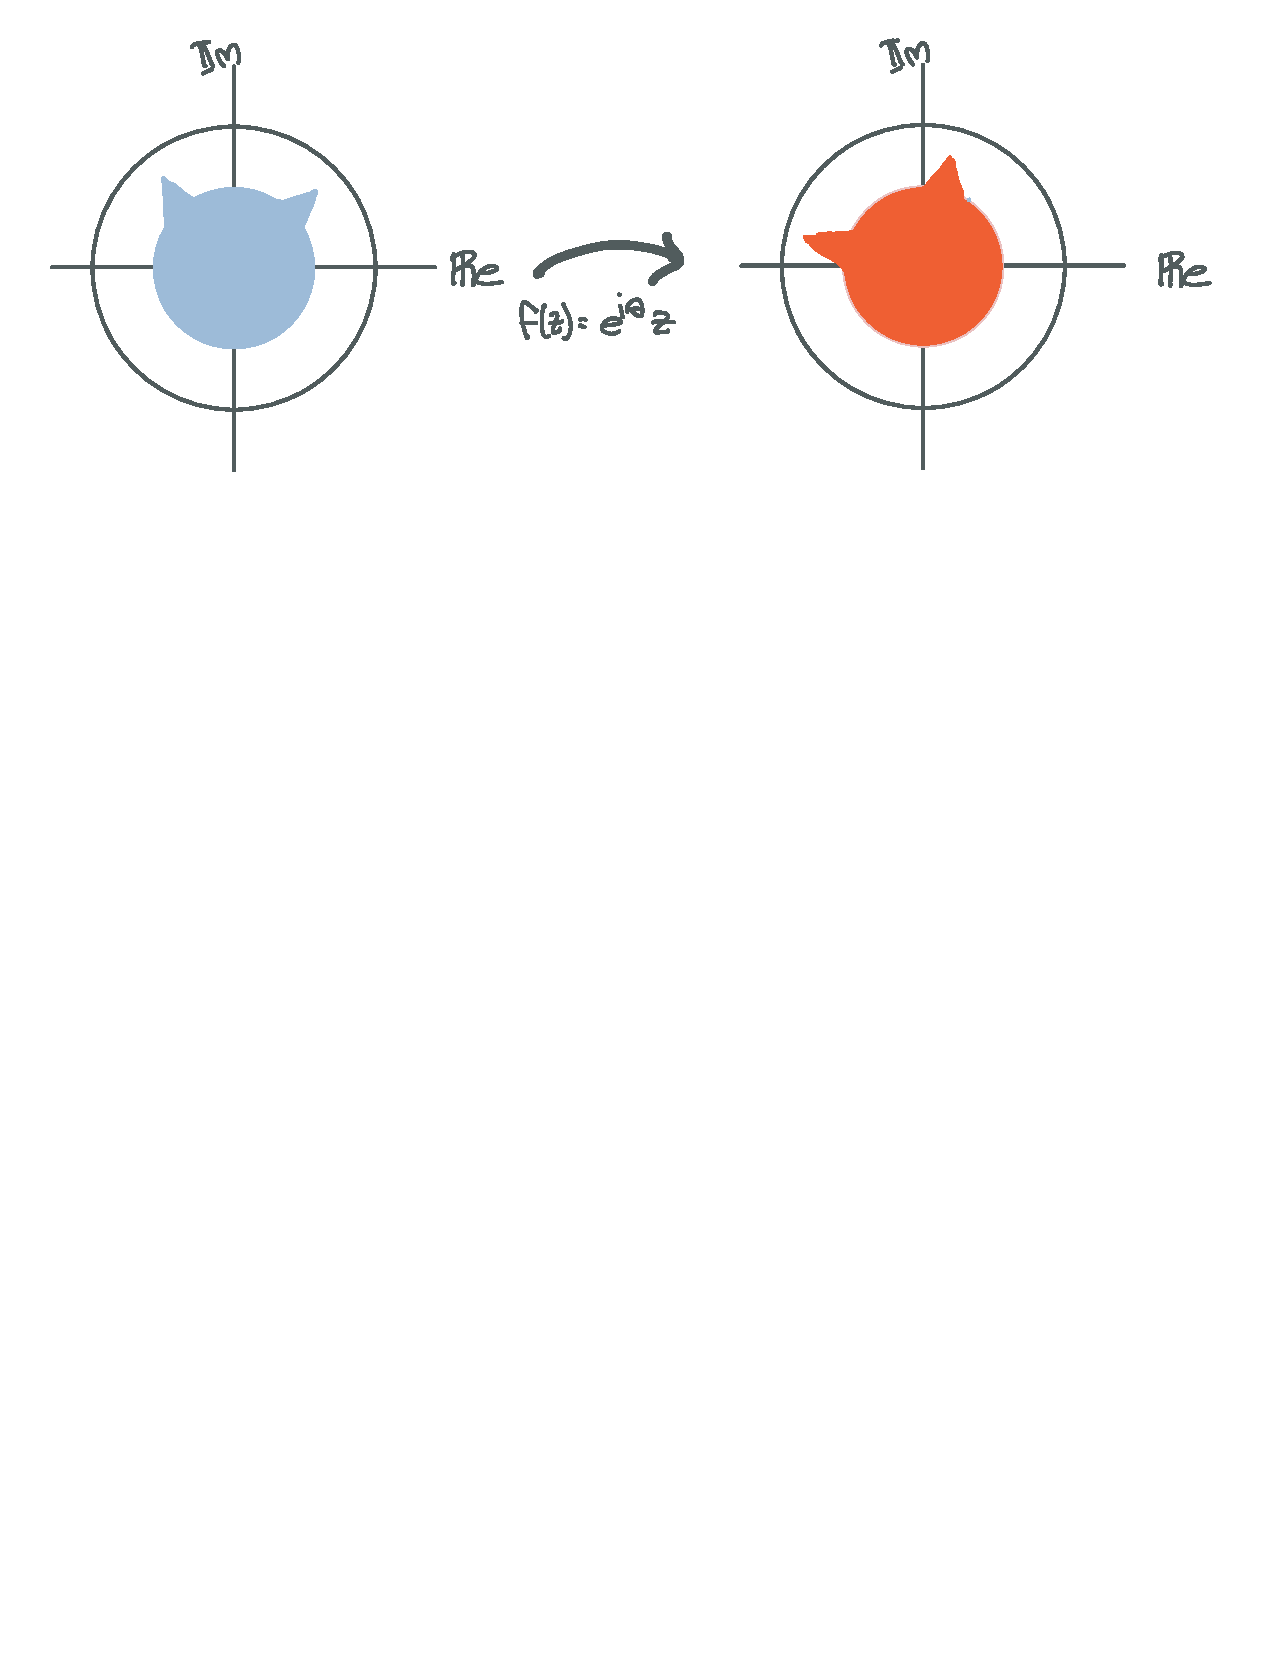
\includegraphics[width=.5\textwidth]{figures/Complex_03_rot.pdf}
\end{center}

\begin{exercise}
What happens to points under $f(z) = z+ z_0$?
\end{exercise}


\begin{example}
Now consider the simplest non-trivial polynomial, the function that squares its argument:
\begin{align}
  f(z) =  z^2 \ .
\end{align}
For a point $z = \rho e^{i\theta}$, $f(z)  = \rho^2 e^{2i\theta}$. This squares the modulus (length) of each point and rotates according to how much the point is already rotated relative to the positive real axis.
\begin{center}
% 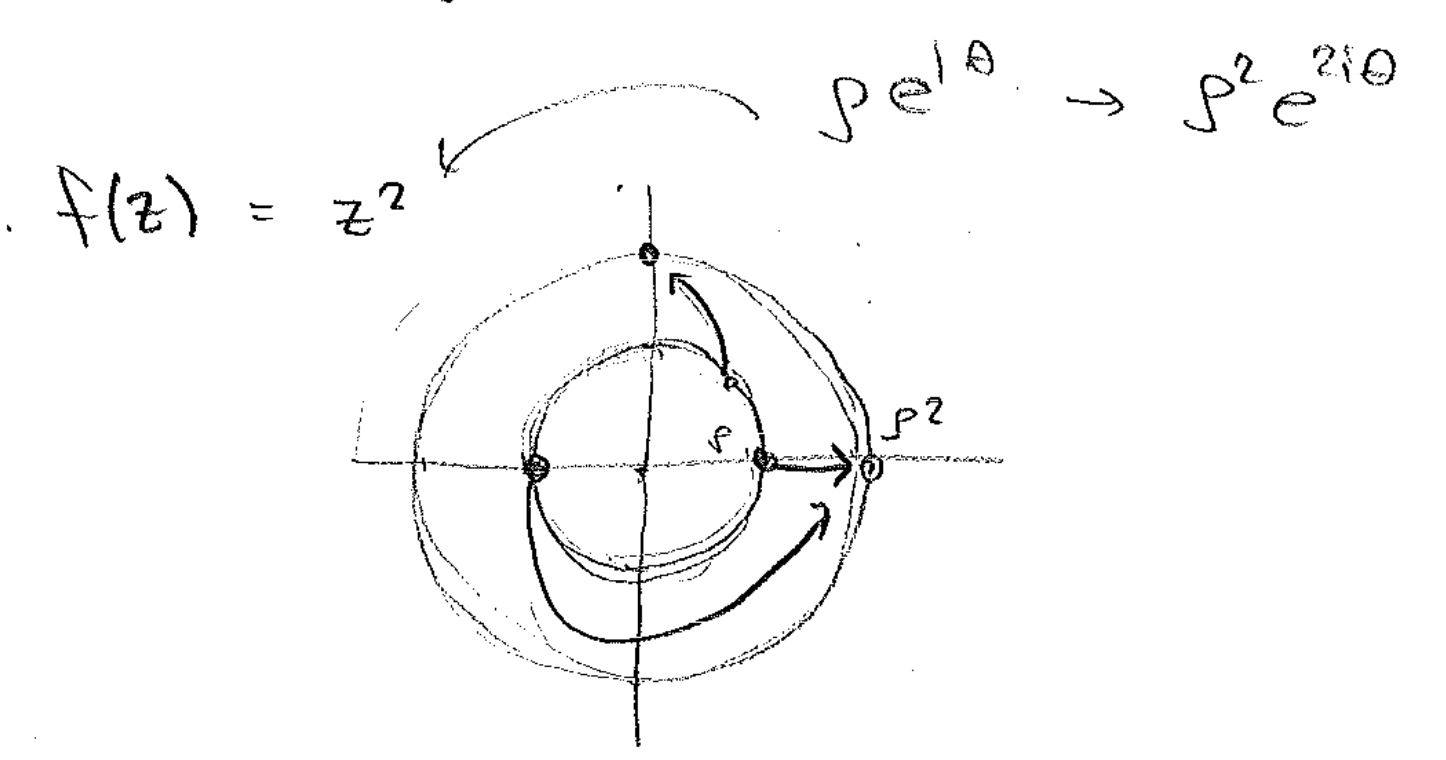
\includegraphics[width=.7\textwidth]{figures/lec13_map2.png}
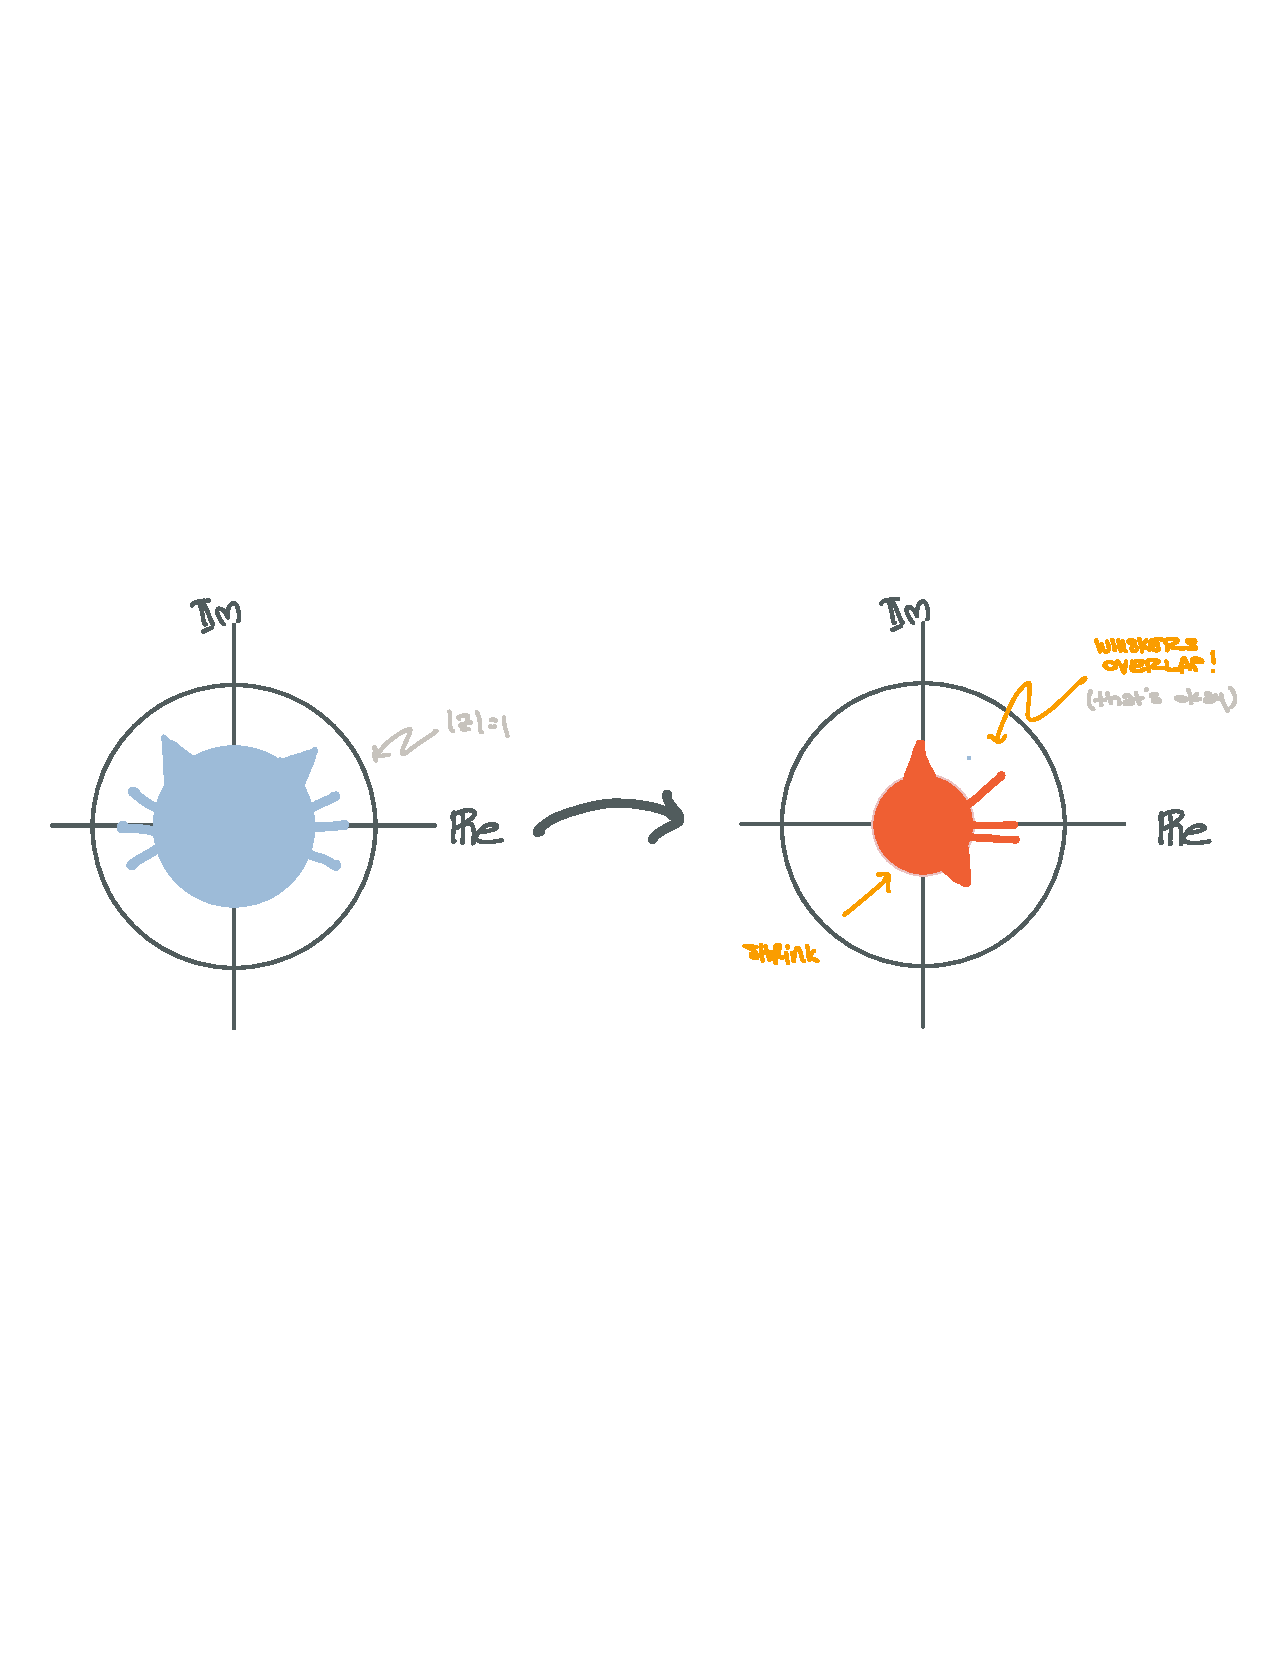
\includegraphics[width=.7\textwidth]{figures/Complex_03_sq.pdf}
\end{center}
Points that are inside the unit circle get pulled closer to the origin while points outside the unit circle are pushed away from the origin.  Points in the first quadrant (positive real and imaginary parts) are sent to points in the upper half plane (positive imaginary part).
\end{example}

In the above example of $f(z)= z^2$, note that some points in the domain are mapped to the same points in the image: $f(-1) = f(1) = 1$. That's perfectly fine: different points can be mapped to the same point under a function---there's only a problem when the same point is apparently mapped to different points in the image. But that never happens... \emph{right?}

\begin{exercise}
Show that under the map $f(z)=z^2$, a vertical line gets mapped onto a parabola:
\begin{center}
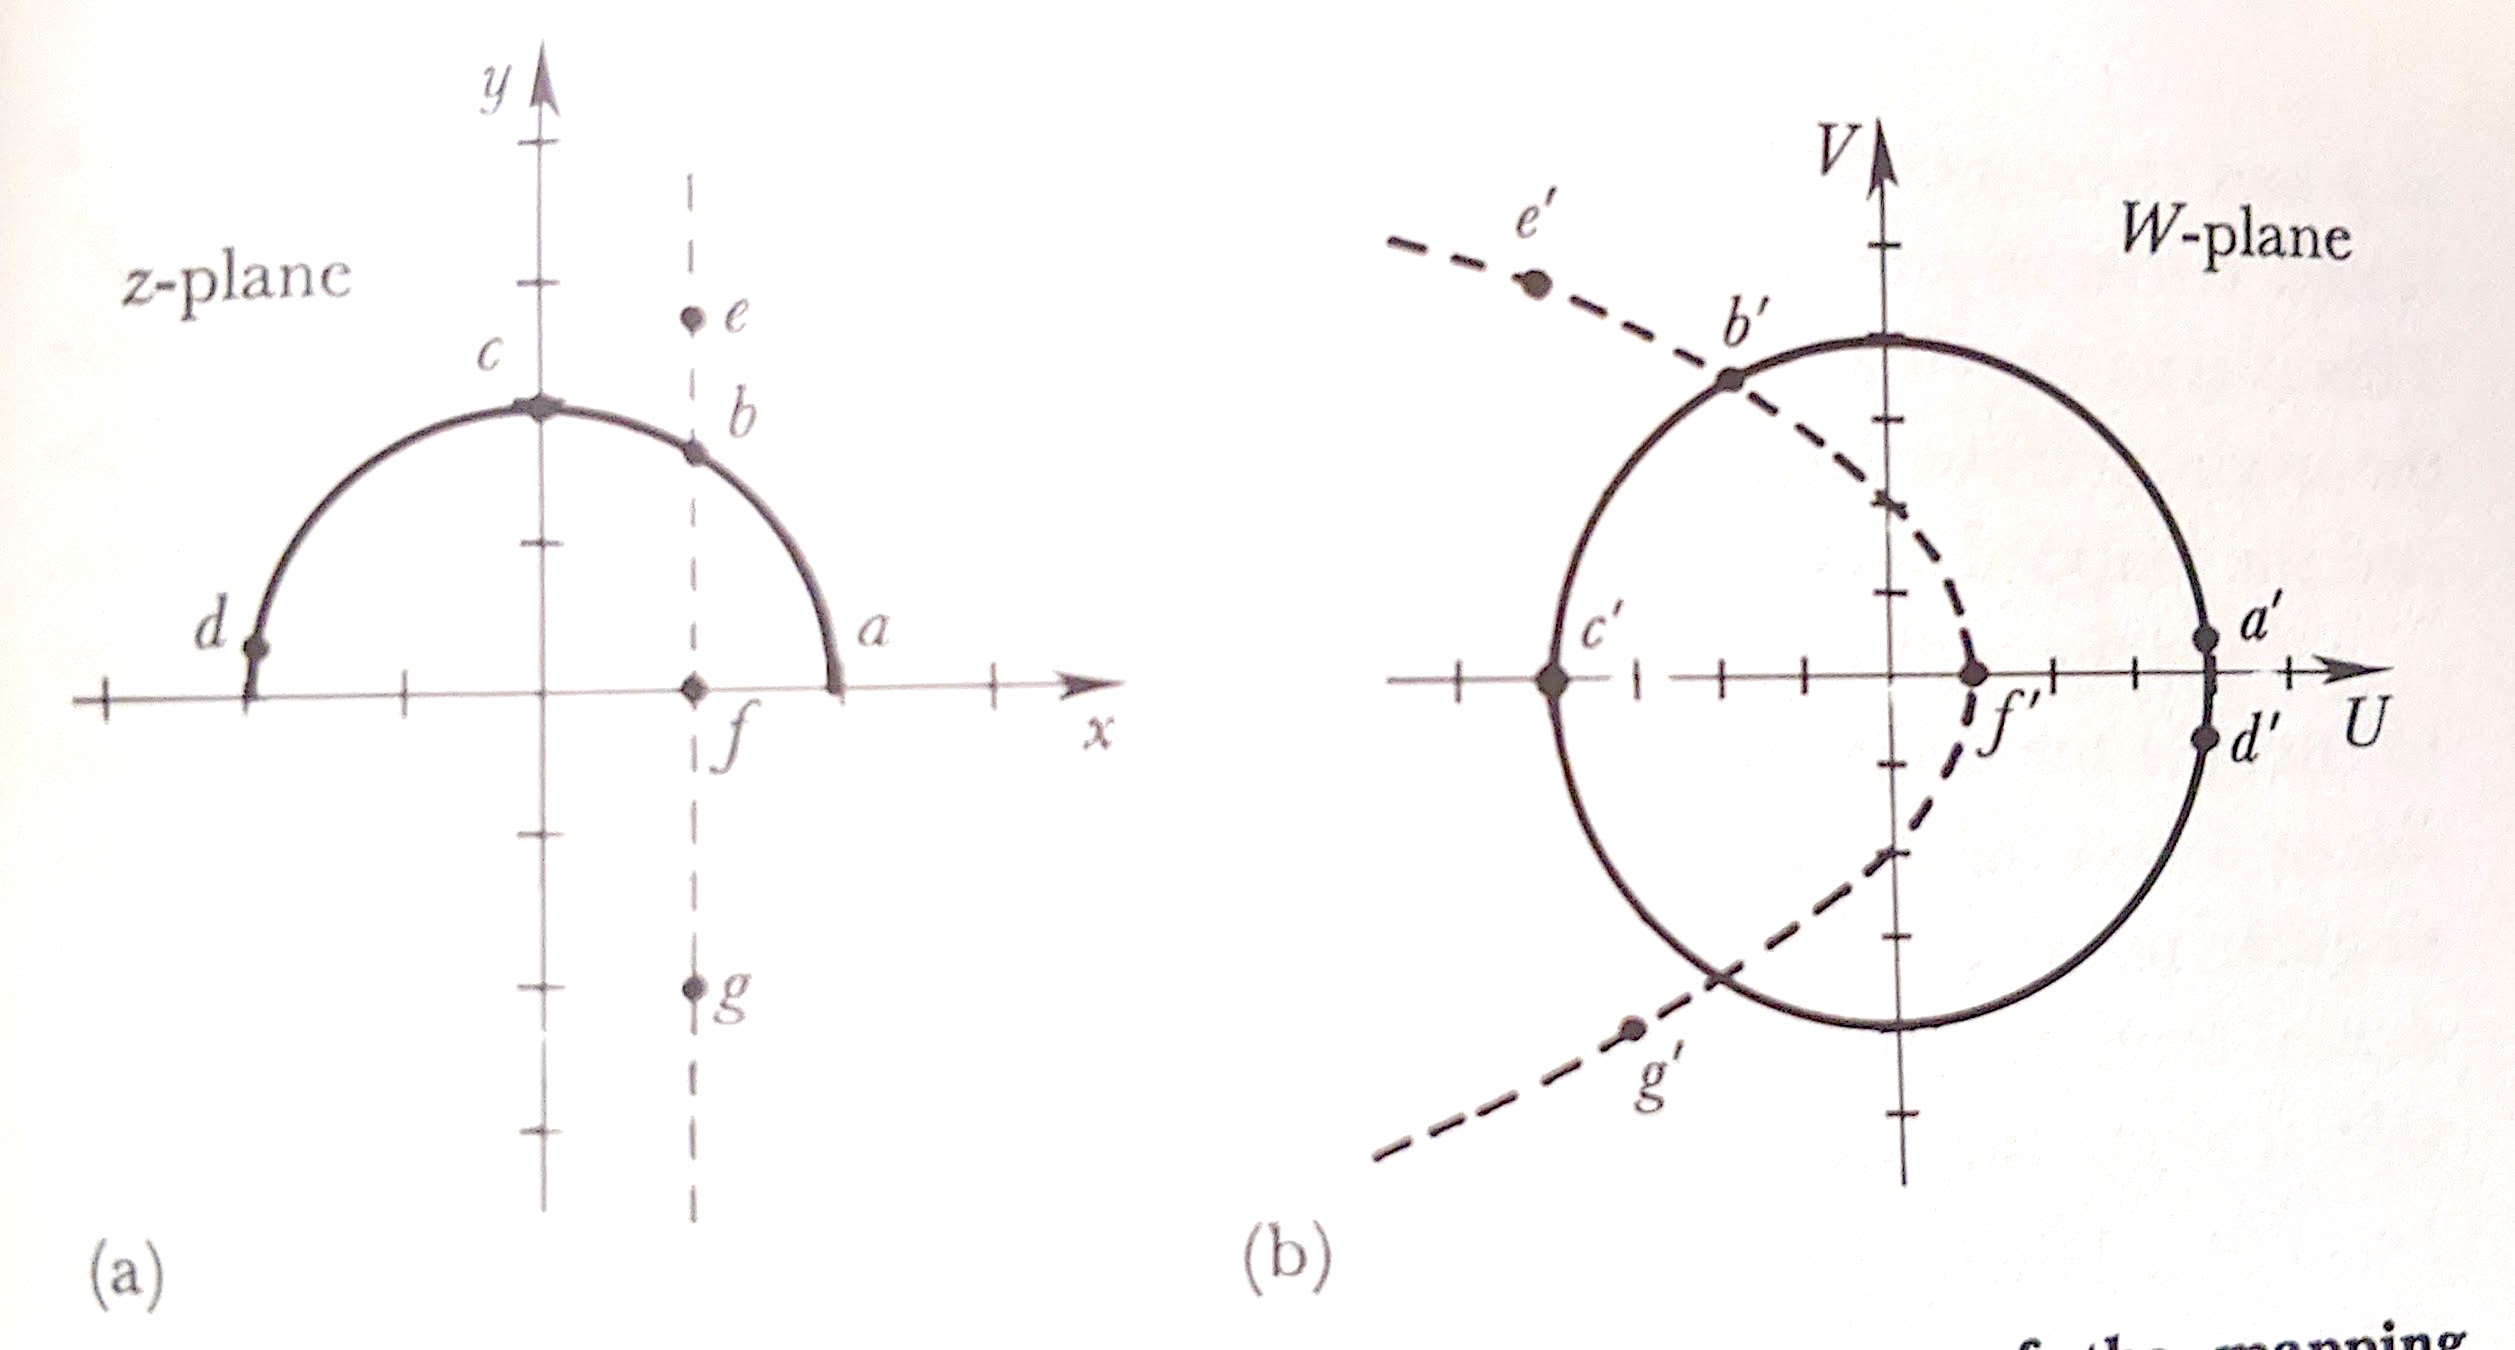
\includegraphics[width=.7\textwidth]{figures/lec13z2.jpg}
\end{center}
Figure from Matthews and Walker, points $a$, $b$, etc.\ are mapped onto $a'$, $b'$ etc. The $W$-plane corresponds to the image of the complex plan under $z^2$.
\end{exercise}

Now let's consider a curious case. What about the square root function?
\begin{align}
  f(z) = \sqrt{z} \ .
\end{align}
Something very weird happens here. Consider a closed path $\gamma(t) = e^{it}$ with path parameter $t \in [0,2\pi]$. This just means consider a bunch of points corresponding to $\gamma(t)$ with a bunch of values of $t$ in the specified range. Clearly this corresponds to a circle. However, when we put those points through the square root function, these only map onto \emph{half} of the circle. 
\begin{center}
% 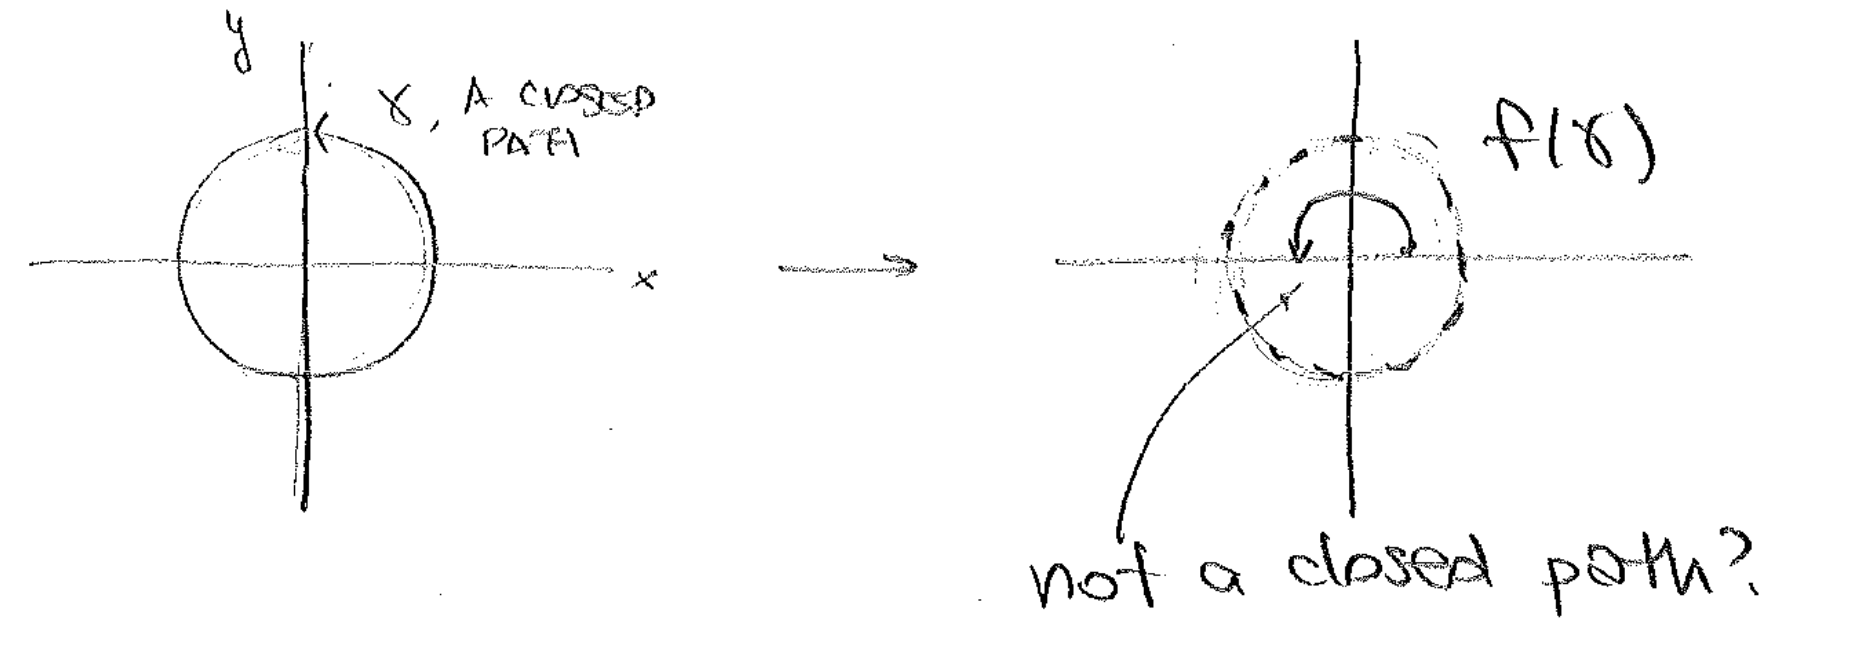
\includegraphics[width=\textwidth]{figures/lec13_map3.png}
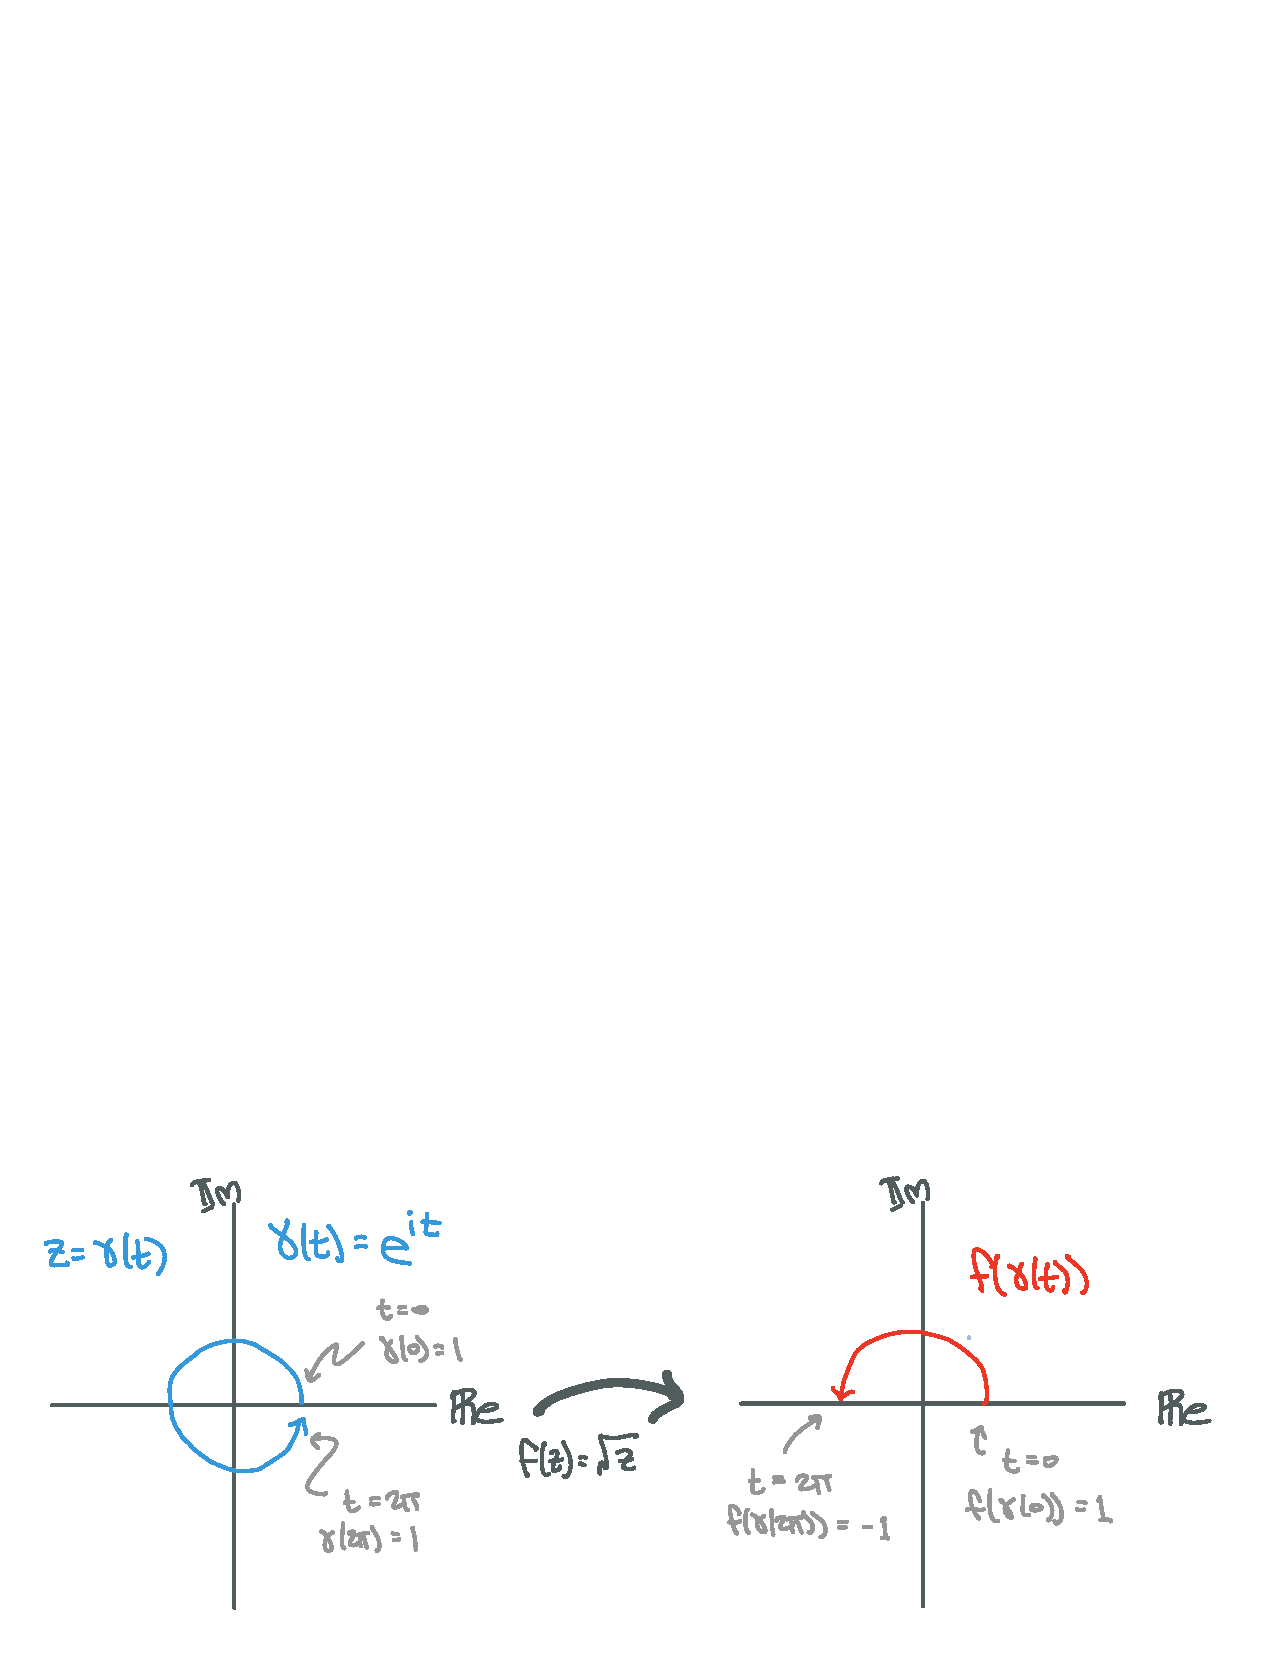
\includegraphics[width=.7\textwidth]{figures/Complex_04_log.pdf}
\end{center}
The technical fact that this happens is not surprising at all, you can see that $f(\gamma(t)) = e^{it/2}$ which only spans the upper half circle. But a deeper question bubbles to the surface: if we're thinking about complex functions as maps of the complex plane to itself, what does it mean that $f(z) = \sqrt{z}$ appears to have `lost' the entire lower half of $\mathbbm{C}$? Or more strangely, how is it that a \emph{closed path} has been mapped to an \emph{open path} with endpoints?

It's clear that if we wanted to reach the \emph{lower} half plane in the iamage, we'd need $\theta \in [0, 4\pi]$. Algebraically that means that $f(\gamma(t)) = e^{it/2}$ covers the entire complex plane \emph{only} if we allow angles from 0 to $4\pi$
\footnote{You may be familiar with another case where `rotating by $2\pi$' only takes you halfway---spinors in relativistic quantum mechanics. You should know that the `double cover' nature of the spinor is (to the best of my view) independent of the present discussion of Riemann sheets. That double cover has to do with the universal cover of the Poincar\'e group. I refer to the literature on the Wigner theorem, see e.g.\ volume 1 of Weinberg's \emph{Quantum Theory of Fields}. For an unrelated cute spinor paper, see \url{https://www.jstor.org/stable/2318771}.}. In some sense, this is totally ridiculous, since $\rho e^{i\theta} \equiv \rho e^{i(\theta+2\pi)}$. I used the $\equiv$ sign because the two sides really are \emph{that} equal.

If, say, $z_1=e^{i\pi/3}$ and $ z_2 e^{7i\pi/3}$ are supposed to be the \emph{same} point, $z_1\equiv z_2$, how is it that $f(z_1) = e^{i\pi/6}$ and $f(z_2) = e^{7i\pi/6}$ so that $f(z_1)\neq f(z_2)$?
\begin{center}
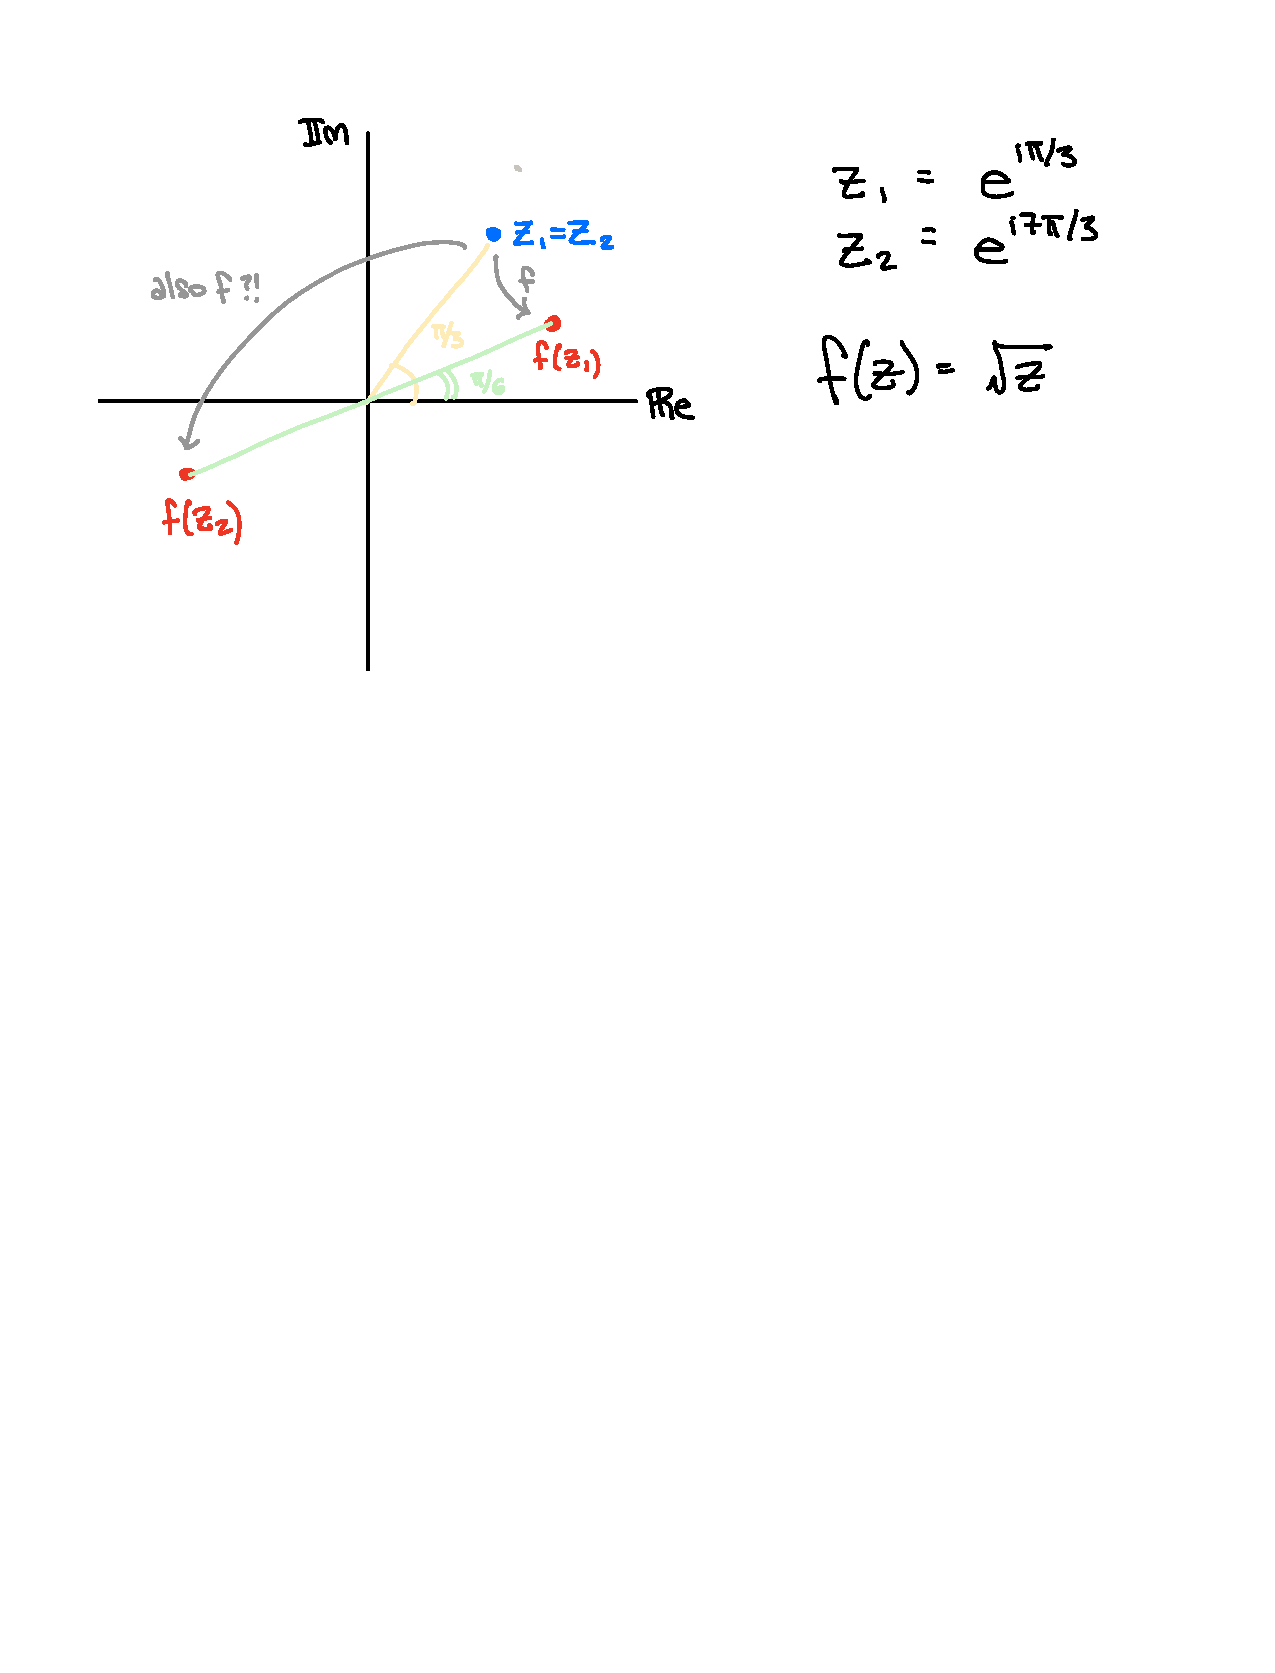
\includegraphics[width=.7\textwidth]{figures/Complex_01_log.pdf}
\end{center}
Stated differently, functions are supposed to be single valued. It appears that $f(z)=\sqrt{z}$ is \emph{multivalued} since the same point $z_1=z_2$ is mapped onto two different points. One way to do this is to \emph{define} additional structure and extend the domain (pre-image) of $f$. In order to do this, we take \emph{two} copies of the complex plane and stitch them together:
\begin{center}
% 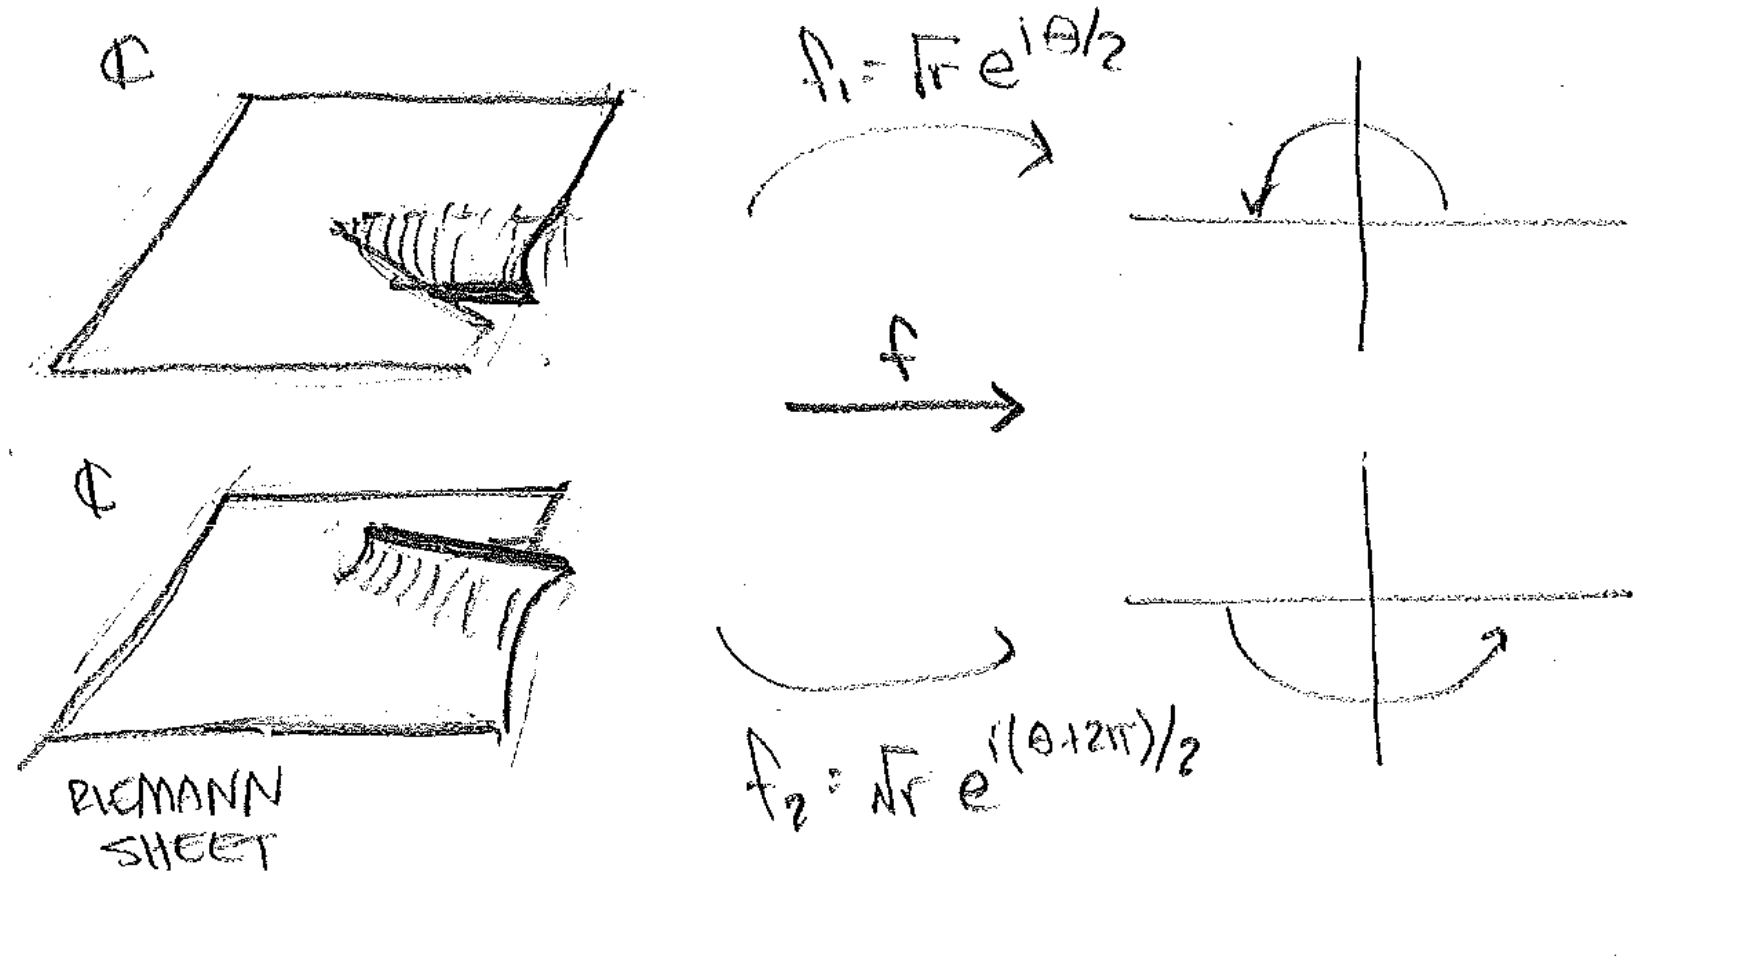
\includegraphics[width=.8\textwidth]{figures/lec13_map4.png}
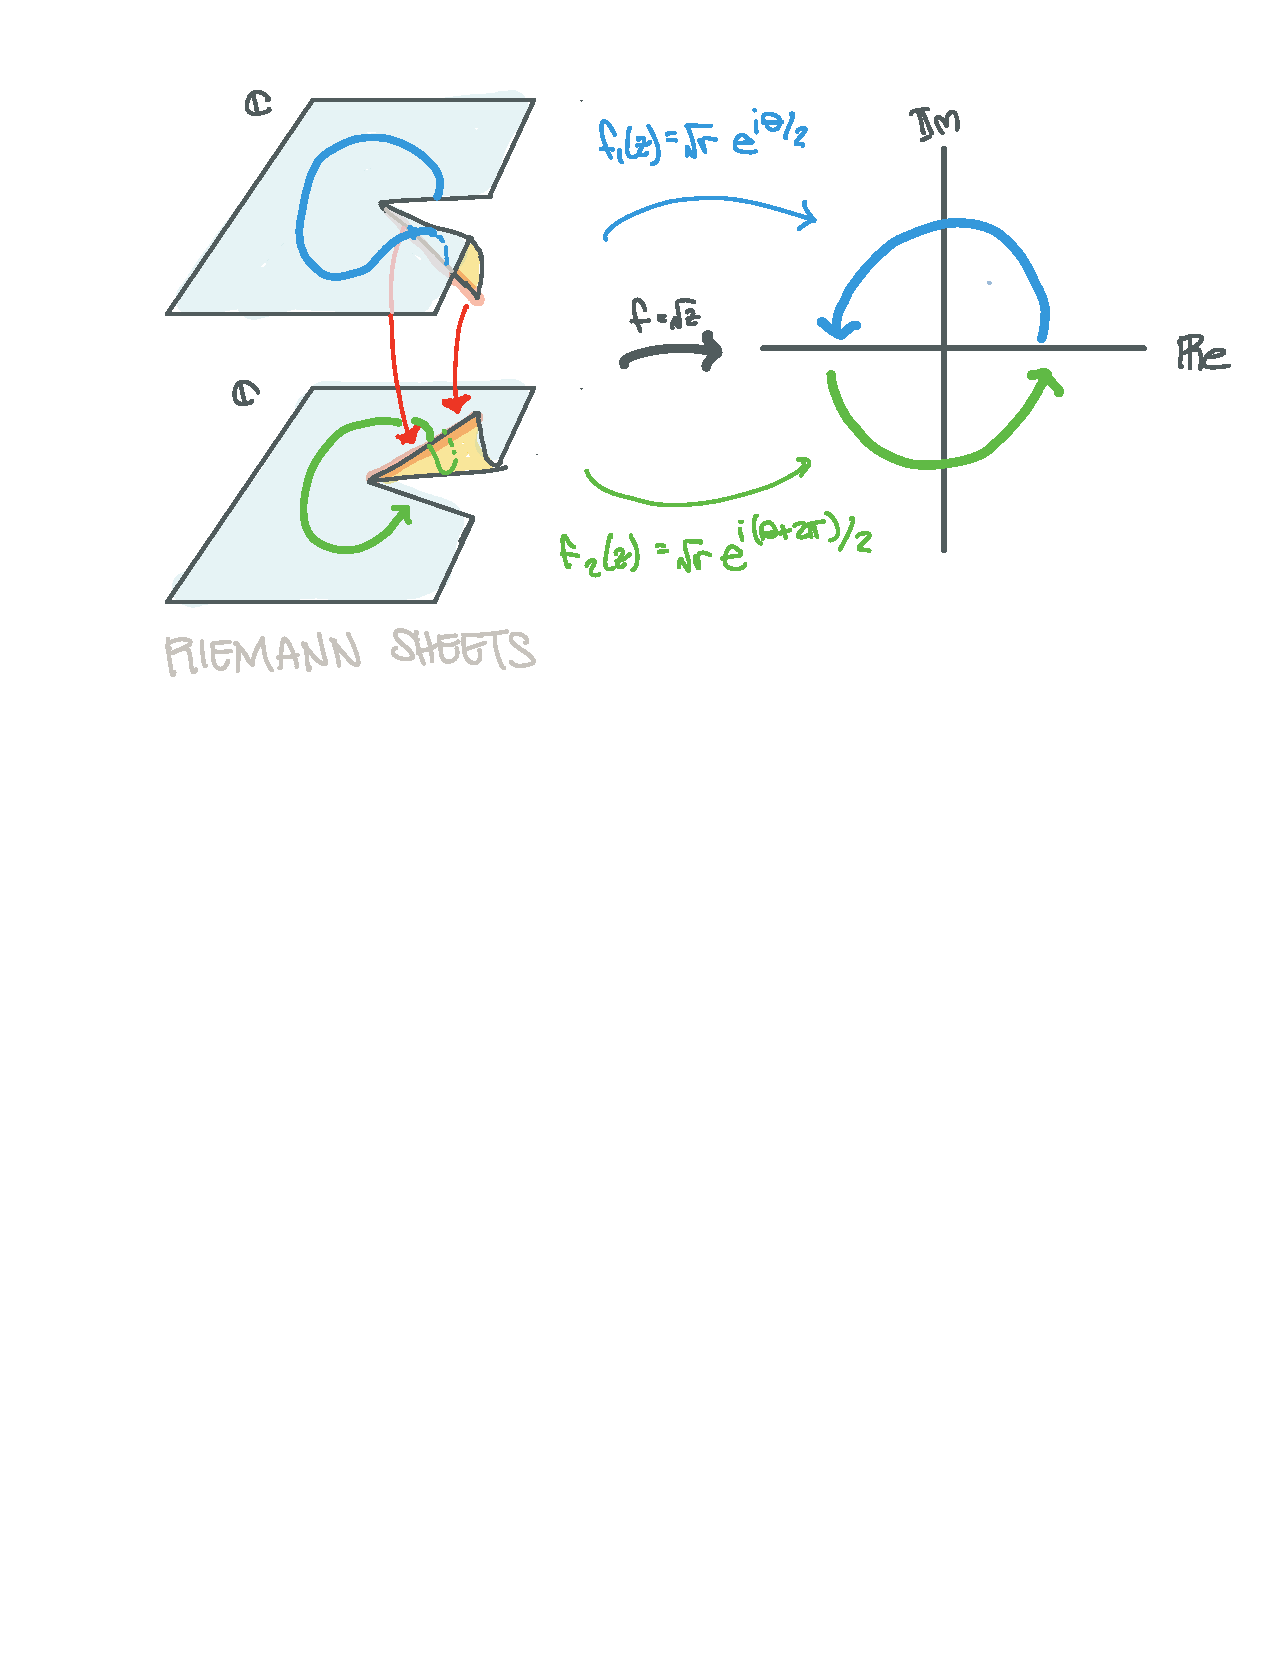
\includegraphics[width=.7\textwidth]{figures/Complex_07_2sheet.pdf}
\end{center}
Each copy of the complex plane is called a \textbf{Riemann sheet}. We `glue' these sheets together by defining that $\rho e^{i(\theta+2\pi)}$ of one sheet maps onto $\rho e^{i\theta}$ of the other sheet. Implicitly this chooses the positive real axis as a place where we \emph{cut} each sheet and glue them together. We call this a \textbf{branch cut}. One could, of course, have chosen the domain of each sheet to be any interval, say $\theta \in [-\pi,\pi]$ and picked a different branch cut ($\theta_\text{branch} = \pi$). 
\begin{exercise}
Is $f(z)=\sqrt{z}$ analytic on the extended complex plane (two Riemann sheets glued together at, say, $\theta=2\pi$)?
\end{exercise}
Take a moment to ponder the above exercise. As you may suspect, the relevant question isn't whether a function $f(z)$ `is analytic,' but rather \emph{where} is that function analytic? Is it analytic (differentiable) anywhere? Sure---when stay within one Riemann sheet, say $\theta\in (0,2\pi)$ and staying away from the boundary, $f(z)=\sqrt{z}$ is perfectly differentiable. Further, there's nothing special about the branch cut---we could have placed it anywhere. Thus it doesn't seem like there's \emph{any} place at which $f(z)$ is \emph{not} analytic. 

This should make sense: analyticity is about whether a function is differentiable at a given point. This is inherently a \emph{local} notion. The misbehavior of $f(z)=\sqrt{z}$---the necessity of Riemann sheets and a branch cut---are \emph{global} issues when we try to explore the \emph{whole} space. The interplay between local properties (like derivatives and Taylor expansions) and global properties (like integrals over a closed surface or topology) is a critical theme in mathematical physics. The function $f(z) = \sqrt{z}$ is analytic everywhere, but that doesn't mean we don't have to be careful. One of the lessons from this section is that the existence of a branch cut can be critically important if you happen to take trajectories that are \emph{loops} in the complex plane. For those who know where this is going: whenever there are branch cuts, you have to be careful with your contour integrals. This typically happens whenever you have a function that is not some series of integer powers of $z$.

As a final example, let's consider the complex logarithm. We'll use the notation of Byron and Fuller and write $\log$ to denote the complex natural logarithm and $\ln$ to denote the `usual' natural logarithm acting on real numbers. For $z=r e^{i\theta}$, the complex logarithm satisfies
\begin{align}
  \log z &= \ln r + i \theta
  \\
  \log(z_1z_2)
  &=\ln(r_1r_2) + i (\theta_1+\theta_2)
  = \log z_1 + \log z_2 \ .
\end{align}
\begin{example}
What does the domain of the complex logarithm look like? As a function, $f(z) = u(z) + i v(z)$, we see that $v(z) = \theta$ and $v(z_1z_2)=\theta_1+\theta_2$. This means that if we take a trajectory that keeps going around the origin, $v(z)$ just keeps increasing\footnote{This is where you can start humming `stairway to heaven.'}. Each time you go around you must be on a new Riemann sheet. 
\end{example}
Rather than having an infinite number of Riemann sheets, an alternative way of thinking about this is to imagine an infinite number of equally valid `complex logarithm' functions labeled by $n$:
\begin{align}
  f_n(z) &= \ln r + i \theta + 2\pi n i \ .
\end{align}
\begin{center}
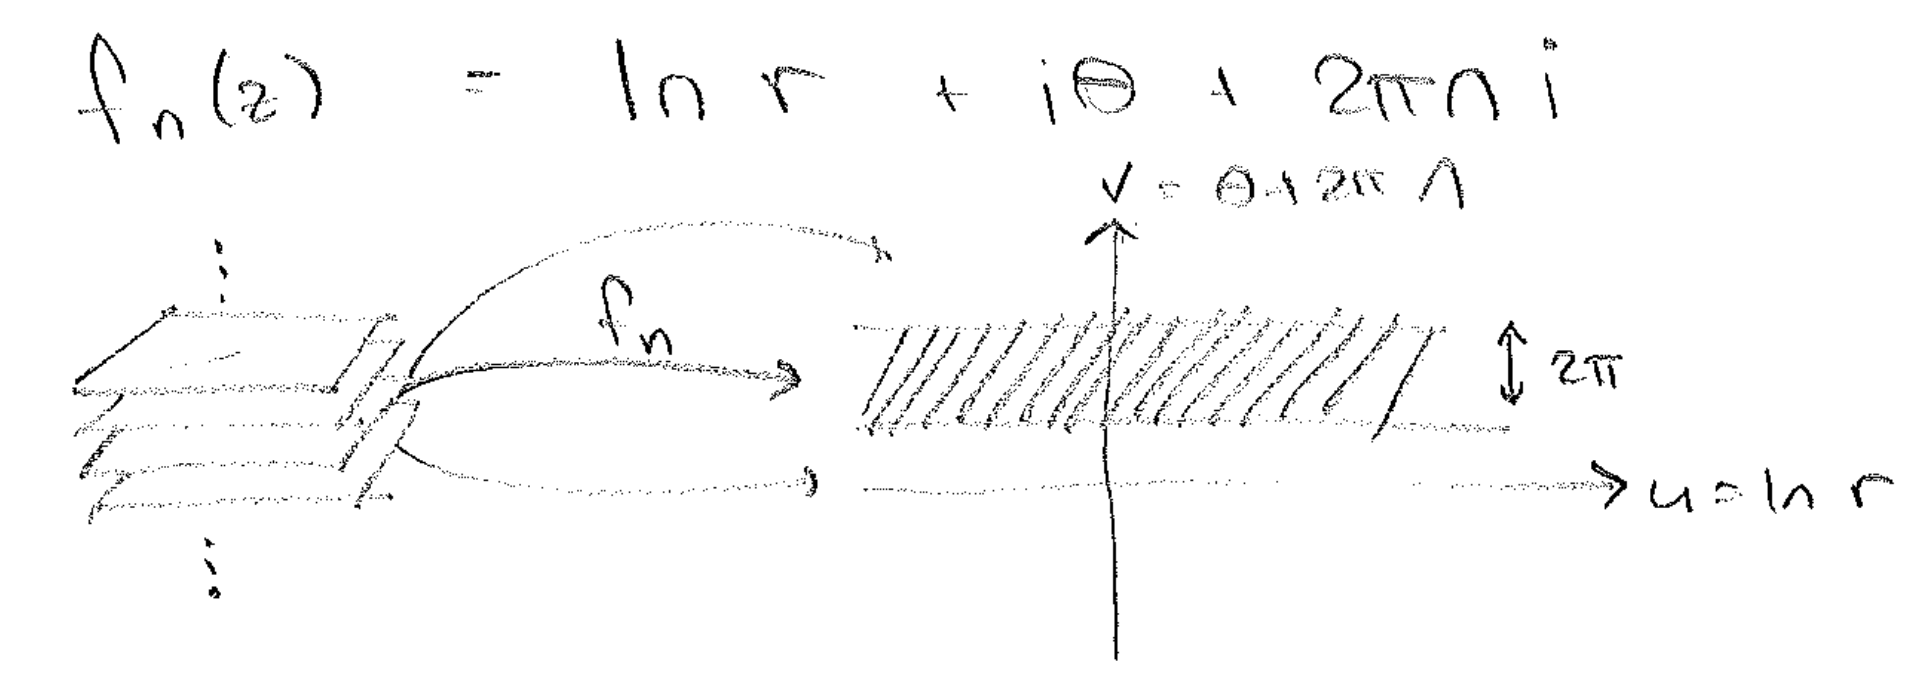
\includegraphics[width=\textwidth]{figures/lec13_map5.png}
\end{center}
The image of the $f_n(z)$ corresponds to a horizontal strip with $v\in \left(2\pi n, 2\pi(n_1)\right)$.
\begin{example}
Is the complex logarithm analytic? Everywhere but at $z=0$.
\end{example}
Let us end by repeating the main point of introducing branch cuts:
\begin{framed}
\begin{center}
Do not integrate across a branch cut!
\end{center}
\end{framed}


\chapter{Complex Integration}

\section{Integration on the Complex Plane}
% StoGo 17.2.1

Let's now focus on integrating analytic functions. Oops, I just misspoke. What I meant to write was that we want to \emph{integrate functions in a region of $\mathbbm{C}$ where those functions are analytic.} Rarely are functions simply `analytic' or `not-analytic.' The functions we care about will be analytic in most places, but non-analytic in others. 

When we integrate on the complex plane, $\mathbbm{C}$, we have to define a \textbf{contour}---this is just the curve, $C$, that we are integrating over. A contour has an \emph{orientation}: the direction along the curve over which one is integrating. Recall that for single variable real calculus,
\begin{align}
  \int_a^b dx\; f(x) = - \int_b^a dx\; f(x) \ ,
\end{align}
you get a relative minus sign if you integrate in the opposite direction.

Integrating along a complex contour is just like a ``line integral'' in $\mathbbm{R}^2$: you are doing a one-dimensional integral in a two[ish]-dimensional space. An integral over the contour $C$ is:
\begin{align}
  \int_C dz\, f(z) &= 
  \int_C (dx + i dy) \, \left[u(x,y)+ i v(x,y)\right]
  \\
  &= 
  \int_C \left[u(x,y)dx - v(x,y)dy\right] 
  + i \int_C \left[u(x,y)dy + v(x,y)dx\right] \ .
\end{align}
Written this way, we are simply doing calculus on $\mathbbm{R}^2$ and keeping track of funny factors of $i$. 
%
It may be helpful to remind ourselves what this means.
\begin{example}\textbf{Integration on the real line.}
As a reminder, let's review integration along the real line, pictorially. Usually we think of the Riemann sum as follows:
\begin{center}
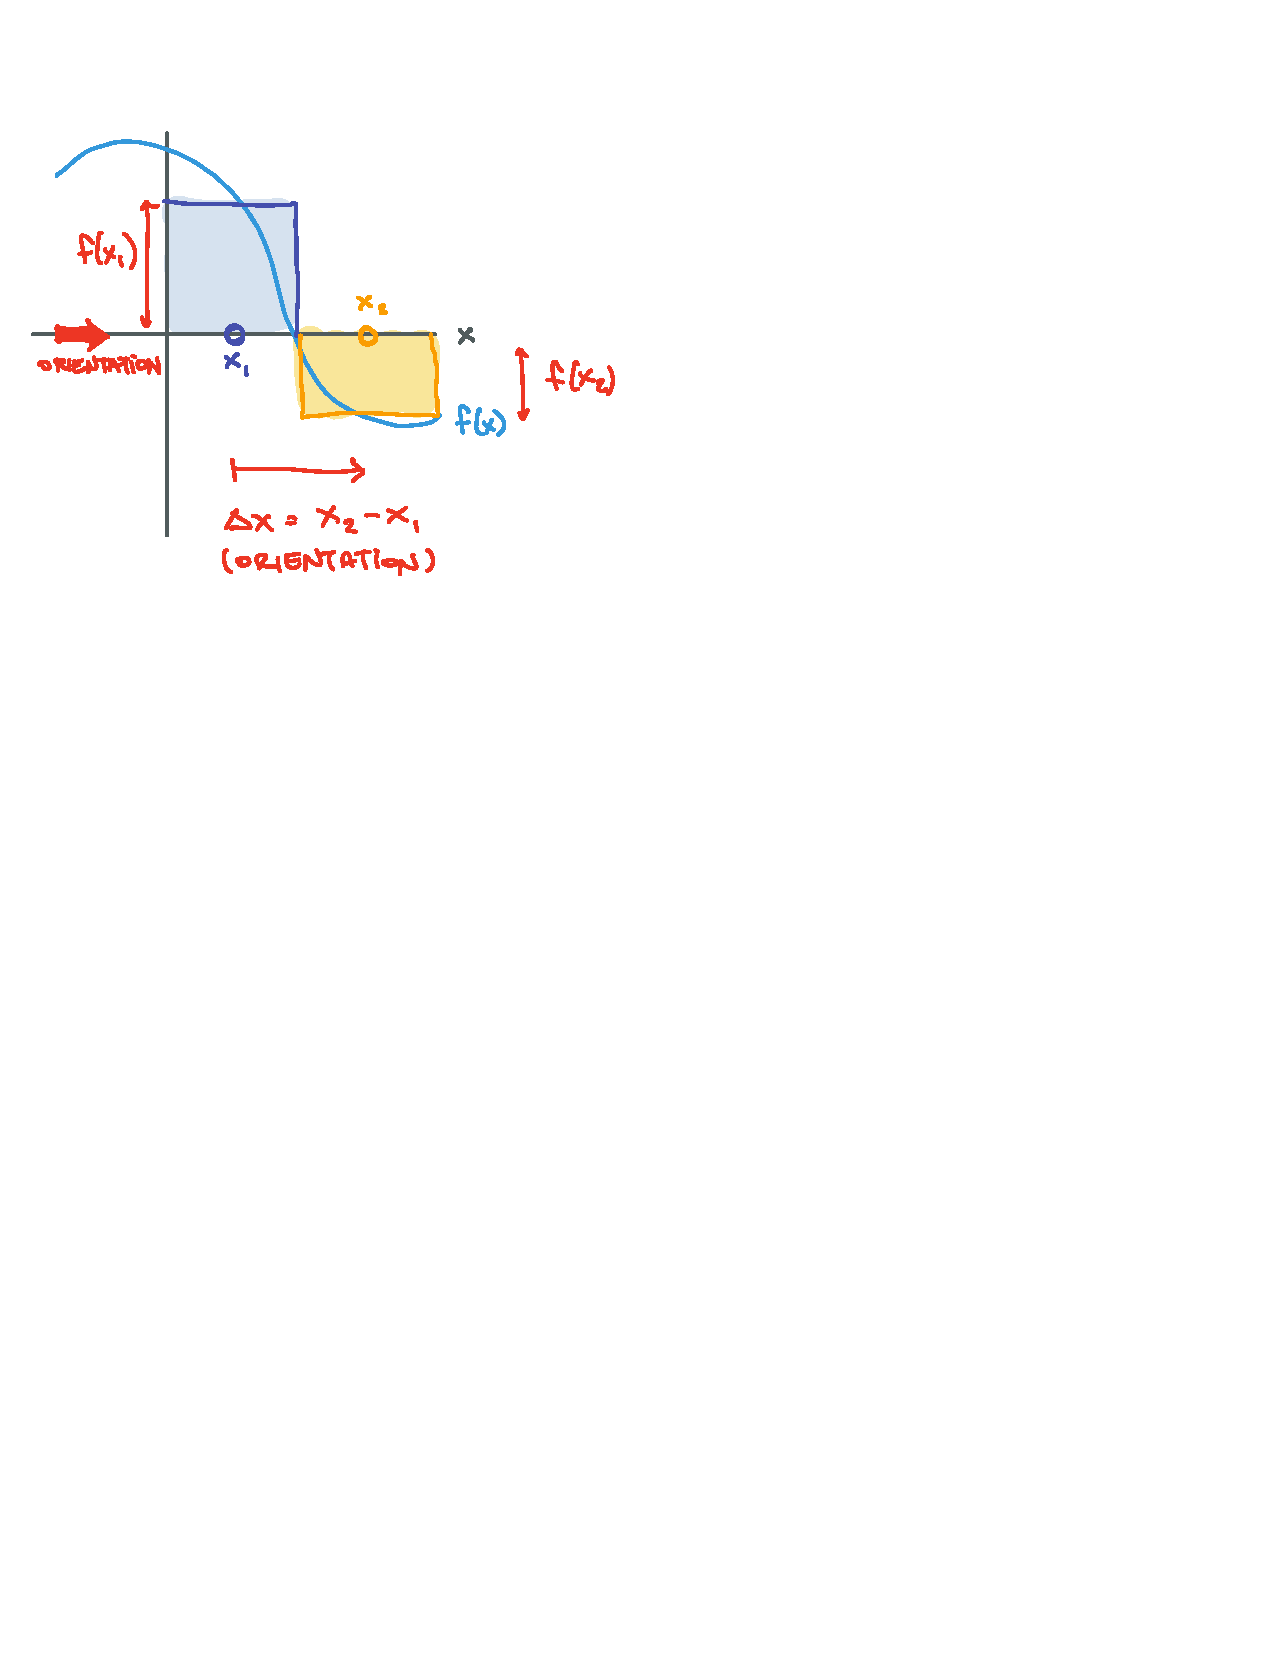
\includegraphics[width=.5\textwidth]{figures/Complex_06_RRiem.pdf}
\end{center}
A more appropriate picture is to draw $f(x)$ on a separate real line:
\begin{center}
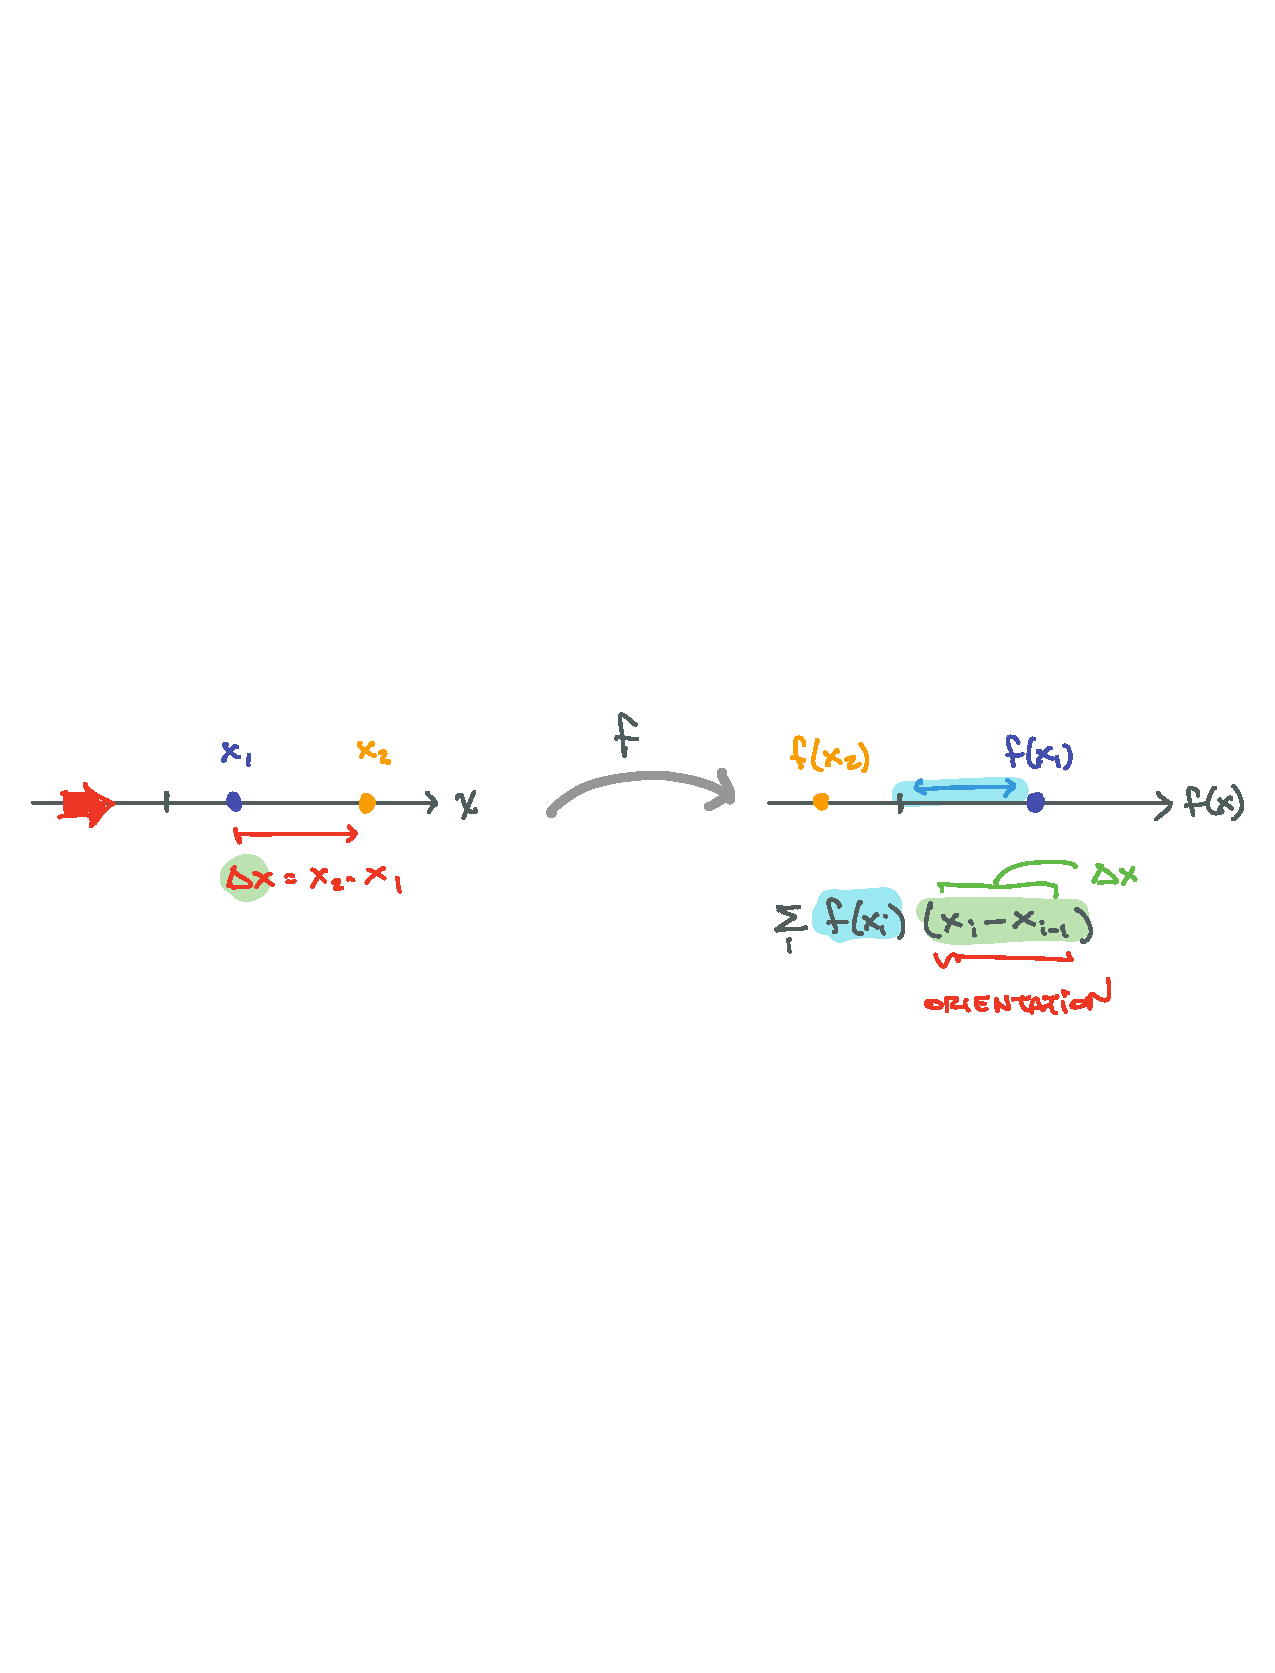
\includegraphics[width=.7\textwidth]{figures/Complex_06_RRiem2.pdf}
\end{center}
The integral is a sum over the function evaluated at some point $f(x_i)$ multiplied by the difference $(x_i-x_{i-1})$. We usually call the difference $\Delta x$ and assume that it is constant and positive. Note, however, that $(x_i-x_{i-1})$ has an \emph{orientation}: there's a sense of direction along the real line. If you go in the opposite direction, you get an overall minus sign.
\end{example}



The integral along a curve can be thought of as two-dimensional version of a Riemann sum. By comparison to the above example, the appropriate picture is this:
\begin{center}
% 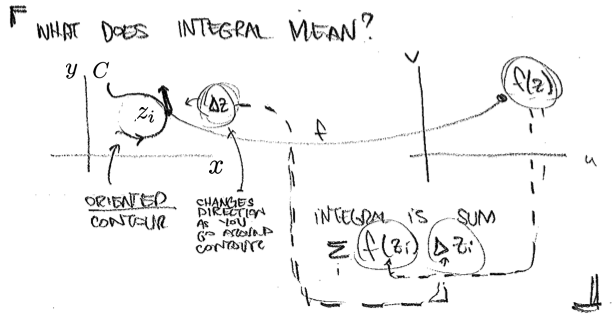
\includegraphics[width=\textwidth]{figures/Lec_2017_12_integral.png}
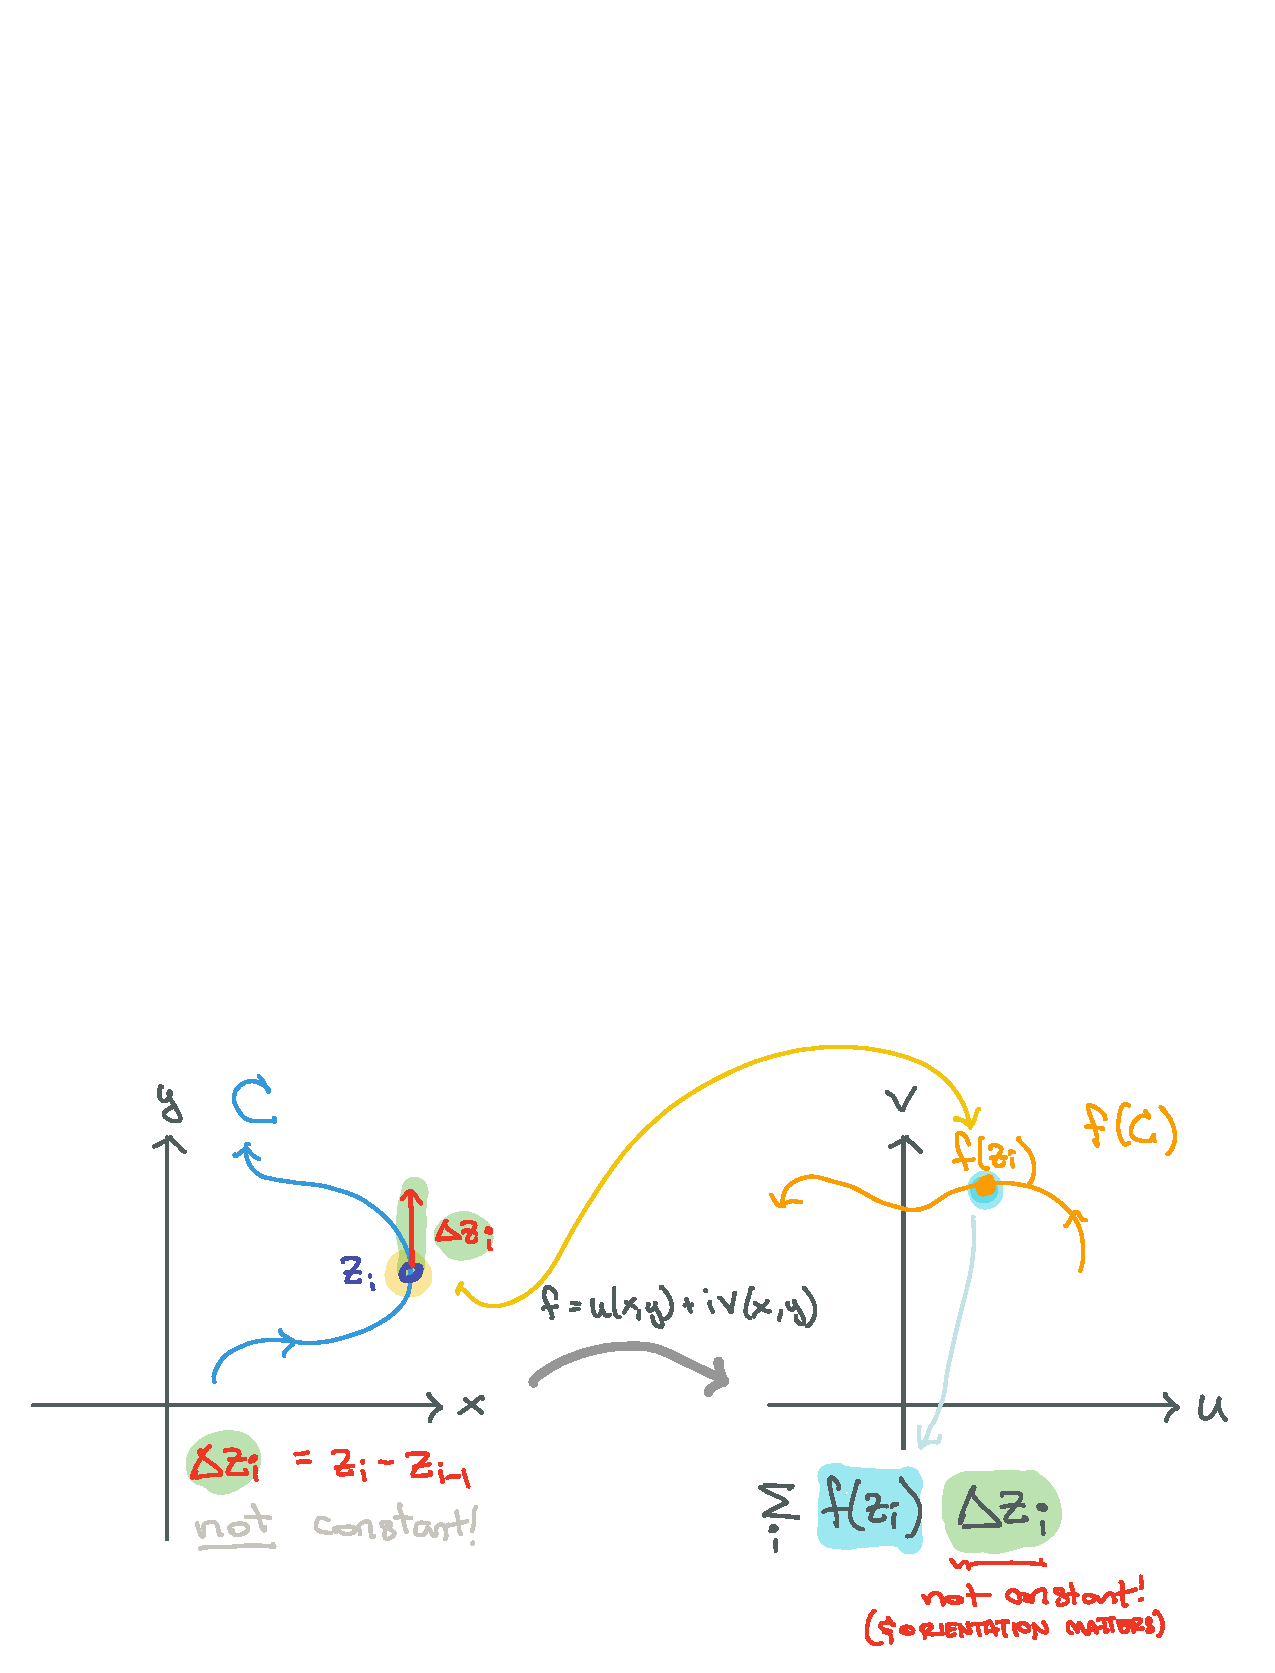
\includegraphics[width=.7\textwidth]{figures/Complex_06_CRiem.pdf}
\end{center}
Note that the complex plane on the right-hand side has coordinate $u(x,y)$ and $v(x,y)$ since $f(z) = u(x,y) + i v(x,y)$. We have written down the generalization of the Riemann sum to $\mathbbm{C}$. 

The one-dimensional real-valued Riemann sum approximated the integral as a sum of terms $f(x_i)\Delta x$. In more than one dimension, the quantity $\Delta x$ is promoted to a `vector'\footnote{As I write this I feel sick to my stomach. In fact, $\Delta x$ is \emph{not} promoted to a `vector,' though it is promoted to something that points in a direction. More properly, it is a [differential] one-form which is more like an \emph{dual vector} in the sense referenced in Section~\ref{sec:analytic:geometric}.}. In other words, we may write
\begin{align}
  \int_C dz\, f(z) = \sum_i \Delta z_i \, f(z_i) \ ,
  \label{eq:complex:integral:Riemann}
\end{align}
where $\Delta z$ has a real and imaginary part: it \emph{points} to a direction in the complex plane. In the picture above, the left-hand side shows the curve $C$ on which we are integrating. Consider some point $z_i$ on the curve. That point is mapped by the function $f$ to a point $f(z_i) = u(z_i)+iv(z_i)$. At that point, the curve also has a differential element, $\Delta z_i$ which is tangent to the curve $C$ at point $z_0$ and has some fixed infinitesimal length for all $i$. The \emph{direction} of $\Delta z$ matters. It contributes to the overall phase of the term $\Delta z_i \, f(z_i)$.
\begin{example}
Consider the function $f(z) = z^2+i$.  Consider a specific point, $z_0 = 1+i$. If we consider different curves $C_i$ that pass through $z_0$, the integral $\int_{C_i}dz\,f(z)$ will have different contributions at $z_0$ depending on the \emph{direction of the curve} as it passes through $z_0$. To see this, consider the specific term in the sum \eqref{eq:complex:integral:Riemann} corresponding to $z_i = z_0$. If the curve $C$ happens to be moving in the positive vertical (pure imaginary) direction, then the contribution to the sum from this point is
\begin{align}
  \int_C dz\, f(z) = \cdots + i\Delta y\left[(1+i)^2 + i\right] + \cdots \ .
\end{align}
However, if the curve $C$ happens to be moving in the horizontal (pure real) direction, the contribution to the sum from this point is
\begin{align}
  \int_C dz\, f(z) = \cdots + \Delta x\left[(1+i)^2 + i\right] + \cdots \ .
\end{align}
\end{example}
\begin{exercise}\label{eq:fundamental:theorem:calculus} \textbf{(Important!)}
Suppose $f$ is itself a derivative of an analytic function, $f(z)=dF(z)/dz$.
Convince yourself that if $C$ is a smooth connected path between two points $z_0$ and $z_N$, then the integral of $f(z)$ over $C$ is
\begin{align}
  \int_C dz\, f(z) &= F(z_N) - F(z_0) \ ,
\end{align}
as you would expect from real-number calculus. This fact probably has some pompous name, like the fundamental theorem of calculus. \textbf{Hint}: write out the Riemann sum, then recall the limit definition of the derivative.\footnote{To make this hint transparent: it helps to write the $dz = z_i - z_{i-1}$ in the integral measure to be the same $dz$ in the definition of the derivative. The whole point is that $F$ is analytic so that $dF/dz$ is uniquely defined at each point and is independent of which direction one is taking the derivative.} 
\end{exercise}


 
\subsection{Cauchy Integral Theorem}
% Cahill p. 160 for a sketch

As we may have referred to earlier---function that are analytic everywhere are too nice. Have you ever read a novel where everyone just got along nicely? Not very interesting. Complex functions are the same---it turns out that integrals of functions around closed curves in domains where they are analytic end up being zero. 

\subsection{Little tiny circles}

Let's show this starting from the simplest possible case. Consider a function $f$ that is analytic in some region $R\in \mathbbm C$. The boundary of this region is a curve $C = \partial R$. First consider the integral of $f$ around a small circle of radius $\varepsilon$ around some point $z_0$:
\begin{center}
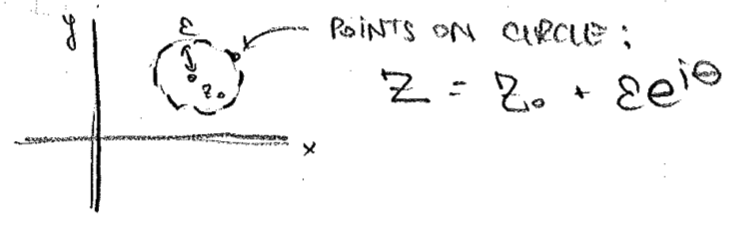
\includegraphics[width=.7\textwidth]{figures/Lec_2017_12_circle.png}
\end{center}
In other words, $C$ can be parameterized by the angle $\theta$. We can write points $z$ on the curve as
\begin{align}
  z(\theta) &= z_0 + \varepsilon e^{i\theta} 
  &
  dz &= i \varepsilon e^{i\theta} d\theta \ .
\end{align}
Note that this parameterization has an orientation: increasing $\theta$ goes counter-clockwise along the circle.
Then the integral around the little circle around $z_0$ is
\begin{align}
  \oint_C dz\, f(z) &= \int_0^{2\pi} i \varepsilon e^{i\theta} d\theta \, f\left( z_0 + \varepsilon e^{i\theta} \right) \ .
\end{align}
Now we observe that since $f$ is analytic around $z_0$, we can differentiate it---which means we can write it as a Taylor expansion about $z_0$:
\begin{align}
  f(z)
   = f(z_0) + f'(z_0)(z-z_0) + \mathcal O(\varepsilon^2) \ ,
\end{align}
where we recognize that $z-z_0 = \varepsilon e^{i\theta}$. Plugging this in gives
\begin{align}
  \oint_C dz\, f(z) &= 
  \int_0^{2\pi} i \varepsilon e^{i\theta} d\theta \, f(z_0) 
  +
  \int_0^{2\pi} i \varepsilon^2 e^{2i\theta} d\theta \, f'(z_0) 
  + \cdots
  \ .
\end{align}
Observe that the only $\theta$-dependence in the integrand shows up in factors of $e^{n i\theta}$ for positive integers $n$. However, we note that
\begin{align}
  \int_0^{2\pi} d\theta e^{in\theta} 
  &= 
  \frac{1}{in} \left(e^{2\pi i n} - e^{0}\right)
  = 0 
  &
  n &\in \mathbbm{Z}_+
  \ .
  \label{eq:complex:theta:integral:trivial}
\end{align}
What we find is that 
\begin{align}
  \oint_C dz\, f(z) &= 0
\end{align}
for the contour $C$ being a small circle around some arbitrary point $z_0$ inside the region $R$ in which $f$ is analytic. 
\begin{exercise}
Convince yourself that it didn't matter that $C$ is a small circle. It could have been any small shape. 
\end{exercise}
Notice that we did not rely on $\varepsilon\to 0$ in order to motivate this argument. The circle didn't actually have to be small. We used $\varepsilon\to 0$ to motivate the idea of truncating the Taylor series. But armed with \eqref{eq:complex:theta:integral:trivial}, we realize that \emph{every} term in the Taylor series will vanish, no matter how high the power since that simply corresponds to some larger positive integer $n$. At this point you should start to wonder whether there may be any loopholes in this argument.




\subsection{Finite regions}

Let's now prove a more general version of this known as the \textbf{Cauchy Integral Theorem}. We use the notation where the boundary of a region $R$ is called $\partial R$. The boundary is assumed to be oriented in the counter-clockwise direction. If $f$ is analytic in a connected region $R \in \mathbbm{C}$ with some boundary $C = \partial R$ , then 
\begin{align}
  \oint_{C=\partial R} dz\, f(z) &= 0 \ ,
\end{align}
even if $R$ is some \emph{finite} region, not just some infinitesimally small circle. From the discussion of the case where $C$ is a little circle, you may have already guessed this. Let's show this more carefully. For any such region $R$, let's break it up into boxes:
\begin{center}
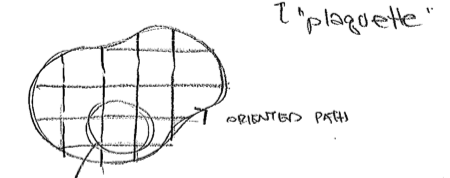
\includegraphics[width=.5\textwidth]{figures/Lec_2017_12_plaquette.png}
\end{center}
The boundary of a region $\partial R$ has some orientation. By convention a positive orientation corresponds to counterclockwise. Now that we've carved up the region $R$ into a grid like Manhattan\footnote{Search for `Manhattanhenge.' It has nothing to do with this course, but this is a photogenic consequence of the Manhattan grid.}, we integrate around the boundary of one of these \emph{plaquettes}:
\begin{center}
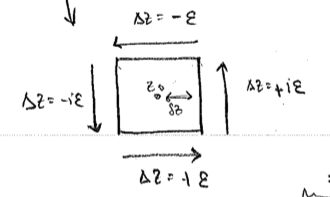
\includegraphics[width=.4\textwidth]{figures/Lec_2017_plaq_int.png}
\end{center}
We've assumed that each plaquette has characteristic size $\varepsilon$. Note that for each side of the plaquette the orientation of $\Delta z$ is different. Let $z_0$ correspond to the center of this plaquette. Since the function is analytic, we can write the function as a Taylor function around the plaquette:
\begin{align}
  f(z) = f(z_0) + f'(z_0) (z-z_0)^2 + \cdots
\end{align}
This means that we can approximate the integral around the square as
\begin{align}
  \oint_\text{plaquette} dz\,  f(z)
  &= 
  f(z_0)
  \left(
    \Delta z_1 + \Delta z_2 + \Delta z_3 + \Delta z_4
  \right)
  + \cdots
\end{align}
where the $\Delta z_i$ are given in the figure above. It should be clear that the sum of the $\Delta z_i$ is zero since opposite sides give equal and opposite contributions. We have shown that to leading order the integral of an analytic function $f$ around a little box around it is zero---not too surprising given our previous result for integrating around a little circle. 
\begin{exercise}
What about the next-to-leading order contribution\footnote{Life advice: ``What about the next-to-leading order contribution'' is a good question to ask whenever you have shown that the leading order contribution is zero.}? Show that the next-to-leading order contribution, which goes like $\sum_i f'(z_0)\delta z_i \Delta z_i$ vanishes. Here the $\delta z_i$ is the separation from $z_0$ to the $i^\text{th}$ side, as shown in the figure above. 
\end{exercise}
The above statement is true about each plaquette. However, note that when we piece the plaquettes together, the sum of the integrals around each little boundary corresponds to the integral around the boundary of the combined region:
\begin{center}
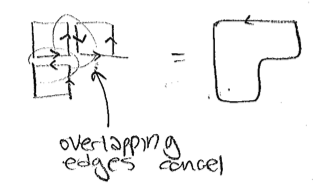
\includegraphics[width=.4\textwidth]{figures/Lec_2017_plaqses.png}
\end{center}
One can see that neighboring boundaries have opposite orientations so that the integrals along those regions cancel. 
%
This means that the integral around a the boundary $C$ of finite region $R$ is equivalent to the sum of the integrals around the little plaquettes that tile that region:
\begin{align}
  \oint_C dz\, f(z) &= \sum_i \oint_{\text{plaquette}_i} dz\, f(z) = 0 \ .
\end{align}
Since the integral around the boundary of each plaquette is zero, the integral along $C$ is zero. This proves the Cauchy integral theorem, which may now be stated as follows:
\begin{quote}
Analytic functions are \emph{so} nice that they're boring.
\end{quote}
In other words, if a function $f$ is analytic in a connected region $R$ and you try to integrate over a closed path $C$ that is inside $R$, then the result is zero. 



\section{An alternative argument}
\label{sec:stokes:theorem:aside}

% \footnote{By the way, this all a generalization of Stokes' theorem: the integral of the derivative of some function $f$ over some domain $D$ is simply the function evaluated on the boundary of the domain, $\partial D$. The $\partial D$ is notation for `boundary of $D$.' The fancy way to write this is
% \begin{align}
%   \int_D df &= \int_{\partial D} f \ .
% \end{align}
% This statement holds for $f$ as a differential $n$-form (the generalization of a one-form and related to an $n$-index tensor) and $D$ is an $n$-dimensional domain. Even if you are not familiar with this nomenclature, please note the qualitative similarities with the integral of a derivative in 1D $\int dx\, (df/dx)$---which is simply the difference of $f$ at the endpoints of the domain, the integral of a curl in 2D---which is related to the `circulation' around the boundary of the 2D domain, and the integral of a divergence in 3D---which is simply related to the flux across the enclosing surface. Vector calculus isn't hard---it's just weird when we treat the 2D and 3D cases as different from the general $n$-dimensional case. 
% }.  

For those who are mathematically inclined, here's a geometrically-motivated argument for Cauchy's integral theorem. If you did Exercise~\eqref{eq:fundamental:theorem:calculus}, then this is already obvious. Consider two points $z_1$ and $z_2$ in a connected region $R$ where a function $f$ is analytic. Now consider any path $C_1$ that connects $z_1$ to $z_2$ and any other path $C_2$ that connects $z_2$ to $z_1$. The orientation matters.
\begin{center}
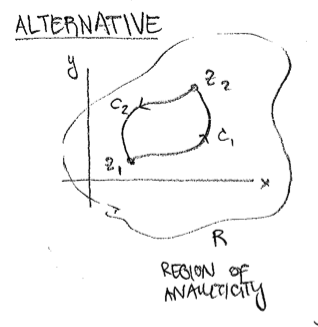
\includegraphics[width=.5\textwidth]{figures/Lec_2017_paths.png}
\end{center}
In the region of analyticity, a function $f(z)$ has an anti-derivative $F(z)$ such that $f(z) = dF(z)/dz$, recall Exercise~\ref{eq:fundamental:theorem:calculus}. Then we know that
\begin{align}
  \int_{C_1} dz\, f(z) &= F(z_2) - F(z_1)
  &
  \int_{C_2} dz\, f(z) &= F(z_1) - F(z_2) \ .
\end{align}
We deduce that the integral of the combined path $C=C_1+C_2$ is zero. The above argument is true without having to specify what $F(z)$ is and for \emph{any} paths $C_1$ and $C_2$ that share common endpoints. We thus prove Cauchy's Integral Theorem.

\paragraph{Commentary}
This argument is highlights a general idea in differential geometry, which is the generalized Stokes' theorem. In words, one can state this as:
\begin{quote}
The integral of the derivative of some function $f$ over some domain $D$ is simply the function evaluated on the boundary of the domain, $\partial D$. The $\partial D$ is notation for `boundary of $D$.'
\end{quote}
Technically it is relevant for the domain $D$ to be sufficiently \emph{nice}; this includes the domain being connected and having a reasonable boundary. Note that the boundary $\partial D$ is always oriented---when we integrate over an interval $[a,b]\in \mathbbm{R}$, the overall sign depends on which boundary is `on top' of the integral and which is `on the bottom.' In other words, it matters if we integrate over $[a,b]$ or $[b,a]$. 

We write formally as follows:
\begin{align}
  \int_D df &= \int_{\partial D} f \ .
\end{align}
Here the domain $D$ is an $n$-dimensional space and $df$ is called a \emph{differential} $n$-\emph{form}\footnote{See \texttt{\href{https://arxiv.org/abs/2009.10356}{2009.10356}} for a recent introduction to the utility of differential forms to elucidate physics at an undergraduate level.}. From the name you should guess that it is related to the idea of a \emph{one-form} as a dual vector; see the optional discussion in Section~\ref{sec:analytic:geometric}.  This is a type of tensor with $n$ indices that is contracted with the `volume form' of the $n$-dimensional space. Formally it looks like this:
\begin{align}
  df &= (\partial_{\mu_1} f_{\mu_2\cdots \mu_n}) \; dx^{\mu_1}\wedge dx^{\mu_2}\wedge\cdots\wedge dx^{\mu_n} \ .
  \label{eq:Stokes}
\end{align}
The quantity $dx^{\mu_1}\wedge\cdots\wedge dx^{\mu_n}$ is the volume form and is an \emph{oriented} $n$-dimensional differential volume element. The funny wedge symbols ($\wedge$) represent an antisymmetric tensor product. This should not be so surprising: recall that the vector triple product $\vec{v}\cdot\left(\vec{w}\times\vec{u}\right)$ is a totally antisymmetric combination of vectors that produces the volume of the parallelogram with edges corresponding to the three vectors $\vec{v}$, $\vec{w}$, $\vec{u}$. This is precisely $\vec{v}\wedge\vec{w}\wedge\vec{u}$. The $n$-dimensional wedge product generalizes this notion to $n$-dimensional volumes. 

On the right-hand side of \eqref{eq:Stokes} is an integral over the \emph{boundary} of $D$. This is an oriented $(n-1)$-dimensional space. The integrand is the differential $(n-1)$-form. We thus see that the integral of $df$ over $D$ is related to a lower-dimensional integral of its primitive, $f$, on the boundary of $D$. 

Stokes' theorem is the underpinning of everything you've seen in vector calculus. In one dimension:
\begin{align}
  \int_a^b dx\, \frac{df(x)}{dx} = \int_{f(a)}^{f(b)} df = f(b)-f(a) \ .
\end{align}
In two dimensions, when you have a vector field $\vec{f}(x)$, the appropriate derivative (and the one that pops out of differential form notation) is the curl, $\nabla\times \vec{f}(x)$. This becomes an integral with respect to the differential surface element $d\hat{S} = \hat{\vec{n}} dS$, which may be chosen to be oriented in the $z$-direction perpendicular to the plane\footnote{Alternatively, $\hat{\vec{n}}$ is the unit normal of the 2D curved surface in a 3D space.}. Then we have the usual  Green's theorem:
\begin{align}
  \int_S dS\, \hat{\vec{n}}\cdot \left(\nabla\times \vec{f}(x)\right) 
  =
  \oint_{C=\partial S} \vec{f}(x)\cdot d\vec{x} 
  \ ,
\end{align}
where $d\vec{x}$ is a differential line element along the oriented curve $C$ that is the boundary of the integration region $S$. Finally, the divergence theorem in 3D relates the divergence of a vector field to its value on the surface:
\begin{align}
  \int_V dV \, \nabla\cdot \vec{f}(x)
  =
  \int_{S=\partial V} dS \, \hat{\vec{n}} \cdot \vec{f}(x) \ ,
\end{align}
where $\hat{\vec{n}}$ is the unit normal vector at each point on the surface $S$ bounding the volume $V$. These three versions of the `fundamental theorem of calculus' all look tantalizingly similar---and here we see that in fact, they're all manifestations of the general Stokes' theorem. 

Observe that the `boundary of a boundary' is nothing. If you have a disc, the boundary is a circle. The circle itself has no endpoints---in contrast to an interval. We can start to see some of the neat features of differential geometry when we look at Stokes' theorem, \eqref{eq:Stokes}, from this perspective. Indeed, one can read Stokes' theorem as a relation between the differential operator $d$ acting on an integrand and the `boundary operator' $\partial$  acting on the space. The `boundary of a boundary = 0' mantra can be loosely translated into `derivative of a derivative' is zero; where we are not being technically rigorous at all. You've already seen variants of this in vector calculus:
\begin{align}
  \nabla\times \nabla f(x) &= 0
  &
  \nabla \cdot \nabla\times \vec{f}(x) &=0 \ ,
\end{align}
and so forth. I used to think vector calculus was very challenging because there seemed to be so many different rules for how to differentiate and integrate. It turns out that differential geometry unifies this nicely into a general mathematical structure that, when applied to specific dimensions of space, produce all of the funny things you learn in undergraduate electrodynamics. It should not surprise you that this mathematical structure has a lot to say about the structure of theories like electrodynamics and gravity\footnote{One of my favorite introductions: \url{https://arxiv.org/abs/hep-th/0611201v1}.}.
\begin{exercise}
To see how this structure shows up in a simple physical system, look up Montgomery's treatment of the Falling Cat Problem. Similarly, Shapere and Wilczek's treatment of swimming animals at low Reynolds number. Wilczek famously won the Nobel prize for his contributions to the gauge theory of the strong nuclear force; a theory based on precisely this type of geometric structure we've discussed here. A final reference is to look up the Parallel Parking Problem, which was a topic of discussion in the first version of this P231 class that I taught in 2016. In that problem, one asks how a car can move transversely given that its only degrees of freedom are to move forward/backward and to turn the steering wheel. For the next two years students raised concerns that this class was hopelessly mathematical---so now here we are at the tail end of an exercise with no specific directions in an optional section of the lecture notes.
\end{exercise}


\section{Cauchy's Integral Formula}

Cauchy's Theorem tells us that integrating functions over domains where they are analytic is boring. Cauchy's Integral Formula\footnote{The name is in contrast to Cauchy's Integral Theorem. At this point you wonder: how is it that Cauchy got his name on everything in this business?} is the first step to something that is decidedly \emph{not} boring. The formula applies to a function $f$ that is analytic in some connected domain and a path $C$ entirely contained in that domain:
\begin{align}
  f(z_0) &= \frac{1}{2\pi i} \oint_C dz \frac{f(z)}{(z-z_0)}  \ .
  \label{eq:cauchy:integral}
\end{align}
This is the statement that the value of some function at some point $z_0$ is related to an integral of the function around the point. In fact, maybe this shouldn't be so surprising: the right-hand side looks like some kind of average of the function in the neighborhood of the function. Given the relation between analytic functions and harmonic functions, this sounds plausible. On the right-hand side there's a factor of $[2\pi (z-z_0)]^{-1}$ which indeed looks like one is averaging over the circumference around the point $z_0$. The factor of $i$ is curious. Those who are familiar with all of this will notice the `famous' combination $(2\pi i)$.

Let is highlight that the integrand on the right-hand side is 
\begin{align}
  g(z) &= \frac{f(z)}{z-z_0} \ .
  \label{eq:g:z:cauchy:integral:theorem}
\end{align}
Unlike $f(z)$, $g(z)$ is absolutely \emph{not} analytic `everywhere' in the region that we're looking at. It is not analytic at $z=z_0$. What's the derivative of $g(z)$ at the singularity? Heck if I know\footnote{Is it infinity? I suppose, but the notion of infinity in complex space can be a little tricky. At any rate, usually `infinity' is not the kind of answer that inspires much confidence.}. This is important because it is our first example of a function that is analytic in a region up to a single point\footnote{%
%
One observant student said that it is not obvious that $g(z)$ is non-analytic at the singularity $z=z_0$. If we define analytic to mean that a function is independent of $z^*$, then it is indeed not clear why $g(z)$ is non-analytic at $z_0$. This ends up being a failure of that definition: the more constructive definition of analyticity is having a unique and well-defined derivative as defined by the limiting procedure, $$\lim_{\Delta z\to 0}[g(z+\Delta z)-g(z)]/\Delta z \ .$$ 
%
}; we say that the function $g(z)$ has a \textbf{pole} at $z=z_0$.\index{pole}

Since the integrand $g(z)$ has a pole, we probably shouldn't integrate over it. No problem, our integration contour $C$ away from $z_0$. However, $z_0$ still punctures our domain over which the integrand is analytic\footnote{We've given our domain a topology. This, by the way, perhaps the one of the lamest things you can give someone. Once when I was a child I was sad when my parents got me a pair of socks for my birthday. I'd have been even more disappointed with topology. At least the socks kept my feet warm.}. To see what this does, let's consider the integral on the right-hand side.
\begin{center}
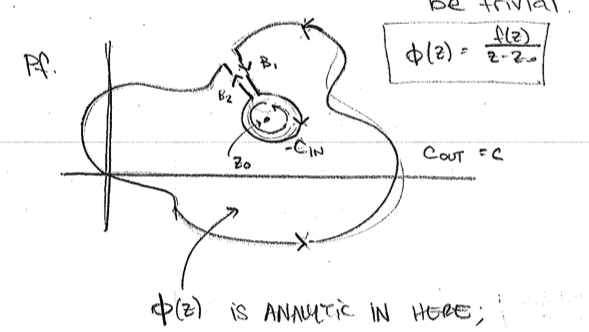
\includegraphics[width=.8\textwidth]{figures/Lec_2017_holes.png}
\end{center}
Let us call $C_\text{out}=C$, the original contour over which we're integrating. It is oriented counter clockwise by assumption. Because we're curious about the singularity at $z=z_0$, let's deform the contour by building a little bridge $B_1$ that heads towards $z_0$, then a little circle $-C_\text{in}$ that goes around the pole\footnote{Note the minus sign! We define $C_\text{in}$ to have positive/counter-clockwise orientation. In the picture above, we see that we traverse this little circle in the clockwise direction, so we put a minus sign on $C_\text{in}$.}, and then a little bridge $B_2$ that returns to $C_\text{out}$ where we originally left it. Clearly the integral over $B_1$ and $B_2$ cancel because
\begin{align}
  B_1 = -B_2
\end{align}
as paths. Note, however, that the region enclosed by the total curve $C_\text{out} +B_1-C_\text{in}+B_2$ is a region in which $g(x)$ is totally analytic. The $-C_\text{in}$ boundary separates the pole from the region enclosed\footnote{An engineer, a physicist, and a mathematician are tasked to optimize the amount of space surrounded by a finite length of fencing. The engineer builds a square pen since that makes it simple to construct. The physicist mumbles something about variational principles and builds a circle, stating that it optimizes the area enclosed for fixed perimeter. The mathematician takes the fence, throws away most of it, and then makes a tiny enclosure. The mathematician then carefully steps inside and says, ``I declare myself to be on the outside.''}. This means that Cauchy's Theorem holds. Because the bridge integrals over $B_1$ and $B_2$ cancel, the theorem tells us that
\begin{align}
  \oint_{C_\text{out}} dz\, g(z)
  -
  \oint_{C_\text{in}} dz\, g(z)
  = 0 \ ,
\end{align}\
where the minus sign came from $\oint_{-C_\text{in}} = - \oint_{C_\text{in}}$. The first term is precisely the right-hand side of \eqref{eq:cauchy:integral}. Apparently the second term is supposed to be $f(z_0)$. We can evaluate the second term along the contour by parameterizing $C_\text{in}$ as
\begin{align}
  C_\text{in}: \quad z(\theta) = z_0 + \varepsilon e^{i\theta} \ ,
\end{align}
which goes around $C_\text{in}$ for $\theta \in [0,2\pi]$. Now watch carefully. The relevant quantities in our integrand are:
\begin{align}
  dz &= i\varepsilon e^{i\theta} d\theta 
  &
  z-z_0 &= \varepsilon e^{i\theta} \ .
\end{align}
Now watch carefully: 
\begin{align}
  \oint_{C_\text{in}} dz\, g(z)
  =
  \oint_{C_\text{in}} dz\, \frac{f(z)}{z-z_0}
  = 
  i\int_0^{2\pi} d\theta f(z) 
  = 2\pi i f(z_0) \ . 
  \label{eq:cauchy:integral:theorem:step}
\end{align}
Note that once we wrote the integral with respect to $d\theta$, this is just an ordinary `real' integral where the integrand happens to have complex numbers in it. What is critical is that the powers of $e^{i\theta}$ canceled. Compare this to what happened in \eqref{eq:complex:theta:integral:trivial}, which was the analogous critical step for showing that the integral of analytic functions vanishes. In \eqref{eq:cauchy:integral:theorem:step} we ended up with \emph{no} factors of $e^{i\theta}$ so that the $d\theta$ integral ended up being non-zero. 
\begin{exercise}
Derive the last equality of \eqref{eq:cauchy:integral:theorem:step}:
\begin{align}
  i\int_0^{2\pi} d\theta f(z) 
  &= 2\pi i f(z_0) \ .
\end{align}
Why are we able to insert $f(z_0)$ in place of $f(z)$? Does this depend on the smallness of $\varepsilon$? (Answer: no.) {Hint}: $f(z)$ is analytic, which means it admits a Taylor expansion. Show that only the zeroth order term contributes, independently of how small $\varepsilon$ may be.
\end{exercise}

Putting this all together gives the desired result,
\begin{align}
  f(z_0) = \frac{1}{2\pi i}\oint_C dz\, \frac{f(z)}{z-z_0} \ .
  \label{eq:cauchy:integral:theorem}
\end{align}

The star of this discussion is not the analytic function $f(z)$; rather it is the analytic-up-to-a-pole function $g(z)$. Unlike our \emph{boring} scenario of functions that are analytic in a given domain, interesting stuff happens when our functions have singularities. We get to live dangerously and dance around theses singularities. In general, we will refer to singularities that go like $(z-z_0)^{-n}$ to be poles at $z=z_0$. The positive integer $n$ is called the order of the pole. The case $n=1$ is called a \textbf{simple pole}.

\section{From Taylor to Laurent}

Functions with poles are clearly not analytic \emph{everywhere}. However, they're pretty close to being analytic. They're analytic except for isolated poles. A function that is analytic up to poles is called \textbf{meromorphic}. If you're like me, you should classify these as \emph{nice, but not too nice} functions. They're just not-nice enough to be interesting. If you're keeping up with the `big picture,' you'll recall that the Fourier transform of a differential operator's Green's function  \eqref{eq:Greens:function:Fourier:transform:heuristic} appears to be in this class.

In a region where $f$ is analytic, differentiability meant that one could write a Taylor expansion: a series of terms that go like $(z-z_0)^n$ for positive integers $n$. When $f$ is merely \emph{meromorphic}, the Taylor expansion is generalized to a \textbf{Laurent expansion}:
\begin{align}
  f(z) = \sum_{n=-N}^\infty  a_n(z_0) (z-z_0)^n \ ,
\end{align}
where $N$ is the order of the pole at $z_0$ (if there is one). 

In a Taylor expansion, the coefficients of each term are simply related to derivatives:
\begin{align}
  \left.a_n(z_0)\right|_{n>0}
  = 
  \frac{1}{n!}\left.\left(\frac{d}{dz}\right)^n f(z)\right|_{z_0} \ .
\end{align}
There's no pithy closed-form expression for the Laurent coefficients. For meromorphic functions, one can be a little clever. Suppose a meromorphic function $f$ has poles at some number of points $\{z_i\}$. The pole at $z_i$ has order $N_i$, so that
\begin{align}
  f(z) = \frac{h(z)}{(z-z_1)^{N_1}(z-z_2)^{N_2}\cdots} \ ,
\end{align}
where $h(z)$ is an analytic function over the complex plane that does not have any factors of $(z-z_i)$---or else the above expression would simplify by canceling these factors in the numerator and denominator. The key trick is that if we want to do a Laurent expansion about a particular pole $z_1$, then we may write
\begin{align}
  f(z) &= \frac{g(z)}{(z-z_1)^{N_1}}
  &
  g(z) &= \frac{h(z)}{(z-z_2)^{N_2}(z-z_3)^{N_3}\cdots} \ .
\end{align}
While $g(z)$ is not analytic everywhere, it {is analytic} at $z_1$. This means we can do a Taylor expansion about $z_1$:
\begin{align}
  g(z) = g(z_1) + g'(z_1)(z-z_1) + \frac{1}{2!}g''(z_1)(z-z_1)^2 + \cdots \ .
\end{align}
Plugging this into $f(z)$ gives precisely the Laurent expansion:
\begin{align}
  f(z) &= \frac{1}{(z-z_1)^{N_1}}
  \left[
  g(z_1) + g'(z_1)(z-z_1) + \frac{1}{2!}g''(z_1)(z-z_1)^2 + \cdots
  \right]
  \\
  &=
  g(z_1)(z-z_1)^{-N_1} 
  + g'(z_1)(z-z_1)^{1-N_1} 
  + \frac{1}{2!}g''(z_1)(z-z_1)^{2-N_1} + \cdots \ .
\end{align}
The Laurent coefficients of $f(z)$ about $z_1$ are:
\begin{align}
  a_{-N_1}(z_1) &= g(z_1)
  &
  a_{1-N_1}(z_1) &= g'(z_1)
  &
  a_{2-N_1}(z_1) &= \frac{1}{2!}g''(z_1) \ ,
\end{align}
and so forth.

\begin{exercise}
How many terms are in the Laurent expansion of
\begin{align}
  f(z) = \frac{(z-4)^2(z-2i)}{(z+1+i)^2(z-3-i)^2} 
\end{align}
about the point $z = 3+i$? Write out the first few terms.
\end{exercise}


\section{The Residue Theorem: a first look}

Now we arrive at our mail tool. Suppose $f(z)$ is meromorphic in some region of the complex plane. In fact, suppose $f(z)$ has a simple pole at $z_0$; the function $g(z)$ in \eqref{eq:g:z:cauchy:integral:theorem} is a function precisely of this type. Consider the integral of $f(z)$ around a closed contour that goes around the pole once. For example, the pole is in some connected region $R$ and the contour is the boundary of this region, $C=\partial R$. Applying the Laurent expansion about $z_0$ for this meromorphic function $f$ gives
\begin{align}
  \oint_C dz\, f(z) &= \oint_C dz 
  \left[
  \sum_{n<0} a_n (z-z_0)^n + \sum_{n\geq 0} a_n (z-z_0)^n
  \right] \ .
\end{align}
All we have done is separated the positive-power terms of the Laurent expansion from the negative power terms. We know that the positive power terms integrate to zero because those terms are analytic in $R$. Thanks, Cauchy's Theorem.

What about the term with negative powers? Since we assumed that $z_0$ is a simple pole, we know that only the $a_{-1}$ term is non-zero in this Laurent expansion about $z_0$. That means that we can write the integral as
\begin{align}
  \oint_C dz\, f(z) &= 
  \oint_C dz \,
  \frac{a_{-1}}{z-z_0} 
  \ .
  \label{eq:residue:int:step:1}
\end{align}
The coefficient $a_{-1}$ of the Laurent expansion about a pole is called the \textbf{residue}\index{residue} of the function $f$ at the pole $z_0$. We use the notation 
\begin{align}
\text{Res}_f(z_0) = a_{-1} \ .
\end{align}
 


Now recall Cauchy's Integral Theorem. For the sake of clarity, let us write the integral theorem with respect to an analytic-in-this-neighborhood function $h$:
\begin{align}
  \oint_C \frac{h(z)}{z-z_0} = {2\pi i} \, h(z_0) \ .
  \label{eq:integral:of:analytic:in:its:neighborhood:function}
\end{align}
Compare this to \eqref{eq:residue:int:step:1}. This seems to tell us that $h(z_0) = \text{Res}_f(z_0)$ so that we ultimately have
\begin{align}
  \oint_C dz\, f(z) &=  2\pi i  \, \text{Res}_f(z_0) \ .
  \label{eq:residue:int:one:pole}
\end{align}
We will generalize this shortly, but the main idea is in this simple example. Note that \eqref{eq:residue:int:one:pole} is mostly correct, but we were a bit too slick and missed something in our discussion.
\begin{exercise}
What assumption did we make in \eqref{eq:integral:of:analytic:in:its:neighborhood:function} that is not always true? We address this in Section~\ref{sec:complex:cauchy:int:thm:factorizing:be:careful}.
% We assumed that h(z) does not have a (z-z0) factor.
\end{exercise}
If you can identify the $a_{-1}$ coefficient of a meromorphic function at its pole, then you can easily integrate the function around the pole. As long as there aren't any other poles in the neighborhood, it doesn't matter what your contour is as long as you are going around counter-clockwise and you go around exactly once.


\section{The Residue Theorem: more carefully}

The residue theorem is our primary tool for calculating integrals on the complex plane. Let's see how it generalizes. Consider a meromorphic function $g(z)$ with two simple poles:
\begin{align}
  g(z) &= \frac{h(z)}{(z-z_1)(z-z_2)} 
  &
  h(z) \text{ analytic over }\mathbbm{C} \ .
\end{align}
The simple poles are located at $z=z_1$ and one at $z=z_2$. Consider a contour $C$ that encloses both poles. The integral of $g(z)$ along $C$ is simply $2\pi i$ times the sum of the residues of the two simple poles. This is easy to see from dividing $C$ into the sum of two paths:
\begin{center}
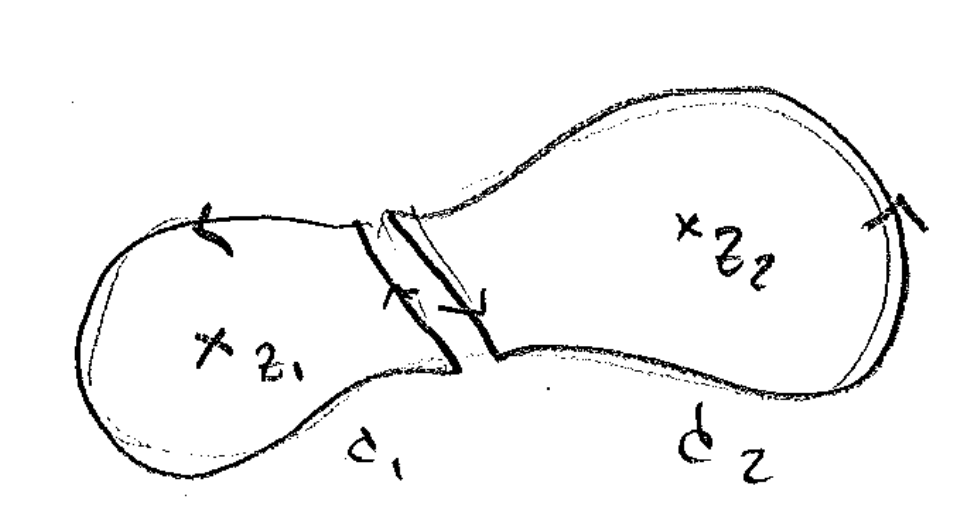
\includegraphics[width=.5\textwidth]{figures/Lec_2017_13_2poles.png}
\end{center}
Here $C_1$ is a closed contour that encloses $z_1$ but not $z_2$. Similarly, $C_2$ is a closed contour that encloses $z_2$ but not $z_1$. Observe that $C_1$ and $C_2$ overlap along a line that separates the two poles. Because both $C_1$ and $C_2$ are positively oriented, the integrals along this line cancel. From this it is clear that
\begin{align}
  \oint_C dz\, g(z) &=
  \oint_{C_1} dz\, g(z) 
  +
  \oint_{C_2} dz\, g(z)
  = 2\pi i\left(\text{Res}_f(z_1) + \text{Res}_f(z_2)\right) \ .
\end{align}
This gives a more general form of the residue theorem. The integral of a meromorphic function $f(z)$ around a closed contour $C$ that is the boundary of some region of the complex plane\footnote{Note that this means that $C$ is positively oriented and only circles around the region once.} is
\begin{align}
  \oint_C dz\, f(z) &= 2\pi i \sum_{i\in \text{poles}} \text{Res}_f(z_i) \ ,
\end{align}
where the sum is over the poles of $f$ at $z_i$ enclosed inside $C$.
\begin{exercise}
How would the residue theorem change if the contour $C$ were oriented in the opposite direction? What if the contour circled the poles multiple times? What if the contour circled some poles some number of times, and other poles a different number of times?
\end{exercise}

\section{Non-simple poles (a case study in being careful)}
\label{sec:complex:cauchy:int:thm:factorizing:be:careful}

So far we've focused only on meromorphic functions that have \emph{simple} poles. What about higher order singularities? Here's a tangible example:
\begin{align}
  \oint_C dz \, f(z) = ?
  &&
  f(z) &= \frac{1}{(z-2i)^2} \ ,
  \label{eq:non-simple:pole:example}
\end{align}
where $C$ is a positively oriented contour that circles the second-order pole $z_0 = 2i$. Because $f(z)$ has no simple pole at $z_0$, it looks like there's no contribution to the integral. To check this, we recall Cauchy's integral formula, \eqref{eq:cauchy:integral:theorem:step}. The reason why simple poles contributed to the contour integral is the observation that for an integer,  $n$, the integral of $e^{in\theta}d\theta$ behaves as follows: 
\begin{align}
  \int_0^{2\pi}d\theta\, e^{in\theta} 
  &=
  \begin{cases}
  0 & \text{\quad if } n\neq 0
  \\
  2\pi  & \text{\quad if } n= 0
  \end{cases} \ .
\end{align}
Following the same in the previous sub-sections, the integral in \eqref{eq:non-simple:pole:example} about a contour $C$ that circles $z_0=2i$ once is equivalent to the integral over smaller contour $C'$ that is a small circle that surrounds $z_0$. Parameterize $C'$ by the angular variable:
\begin{align}
  z(\theta) &= z_0 + \varepsilon e^{i\theta} & dz &= i\varepsilon e^{i\theta} \, d\theta \ .
\end{align}
Then the integral is:
\begin{align}
  \oint_C dz\, f(z) 
  = 
  \oint_{C'} dz\, f(z) 
  = 
  \int_0^{2\pi} i\varepsilon e^{i\theta} d\theta\, 
  \frac{1}{\varepsilon^2 e^{2i\theta}} 
  =
  \frac{i}{\varepsilon}
  \int_0^{2\pi} d\theta\, 
  e^{-i\theta}
  = 0 \ .
  \label{eq:non-simple:pole:eg:zero}
\end{align}
So this is all consistent with the mantra of \emph{find the $a_{-1}$ coefficient of the Laurent expansion, that's the residue}. 

We should be careful, though. If we're too slick we can convince ourselves of wrong things. For example, suppose we wanted to generalize \eqref{eq:non-simple:pole:example} by changing the numerator of $f(x)$:
\begin{align}
  \oint_C dz \, f(z) = ?
  &&
  f(z) &= \frac{h(z)}{(z-2i)^2} \ ,
  \label{eq:non-simple:pole:example:hz}
\end{align}
where $h(z)$ is an analytic function. For the sake of argument, let's assume that $h(z)/(z-2i)^2$ has been simplified so that there are no common factors between the numerator and denominator\footnote{For example, if $h(z)=(z-2i)$ then clearly $f(z)$ has a simple pole at $z_0=2i$ so the integral picks up a non-zero residue.}. One might think that when we shrink the contour from $C$ to $C'$, we can approximate $h(z)= h(z_0)$ so that
\begin{align}
  \oint_{C'}dz\, f(z)
  &=
  \oint_{C'} i\varepsilon e^{i\theta}d\theta\, 
  \frac{h(z_0)}{\left(z-2i\right)^2}
  =
  \frac{i}{\varepsilon}h(z_0)
  \int_0^{2\pi} d\theta\, 
  e^{-i\theta}
  = 0\,?
\end{align}
In general, this argument is \emph{wrong}. It is wrong even though the \eqref{eq:non-simple:pole:eg:zero} happens to be true. 
\begin{exercise}
Can you spot the incorrect assumption?
\end{exercise}
The incorrect assumption is that we could approximate $h(z) = h(z_0)$ because the little circle $C'$ is always close to $z_0$. The intuition is fine, but we weren't careful enough: even though $h(z)$ is analytic everywhere, we should remember write a Taylor expansion:
\begin{align}
  h(z) = h(z_0) + h'(z_0)(z-z_0) + \cdots
\end{align}
Even if our intent is to only keep the first term, it's a good habit to remember that the Taylor expansion contains many terms. Let's see what happens: 
\begin{align}
  \oint_{C'}dz\, f(z)
  &=
  \oint_{C'} i\varepsilon e^{i\theta}d\theta\, 
  \frac{h(z_0)+ h'(z_0)(z-z_0) + \cdots}{\left(z-2i\right)^2}
  \\
  &
  =
  \frac{ih(z_0)}{\varepsilon}
  \int_0^{2\pi} d\theta\, 
  e^{-i\theta}
  +
  {ih'(z_0)}
  \int_0^{2\pi} d\theta
  +\cdots
  \label{eq:non-simple:pole:example:hz:punchline}
\end{align}
While the first term vanishes, the second term is clearly non-zero since it's a contour integral. Indeed, one ends up with
\begin{align}
  \oint_{C'}dz\, \frac{h(z)}{(z-2i)^2}
  = 2\pi i h'(z_0) \ ,
\end{align}
where evidently $\text{Res}_f(2i)=h'(2i)$ is the residue of $f(z)=h(z)/(z-2i)^2$ at $z_0=2i$. 
\begin{exercise}
Why don't higher order terms in \eqref{eq:non-simple:pole:example:hz:punchline} contribute to the contour integral?
\end{exercise}
The purpose of this example was to show that it can be a little tricky to identify the residue of a function by simply `looking at the denominator.' You will derive an explicit formula in your homework. Fortunately, we will rarely consider non-simple poles in this course. 

% Lec 14 2017

Let's go through a few examples. These are from the third edition of Boas, chapter 14.6. 

\begin{example}
Let $f(z)=\cot z$. Find the residue of $f$ at $z=0$. 

To solve this, we can write out the numerator and denominator of the cotangent:
\begin{align}
  \cot z &= \frac{\cos z}{\sin z}
  = \frac{1-z^2/2 + \cdots}{z - z^3/3!} \ .
\end{align}
From this we see that $z\to 0$ is indeed a simple pole, and one may write the residue as
\begin{align}
  \text{Res}_f(0) &= \lim_{z\to 0} z \frac{1}{z} = 1 \ .
\end{align}
\end{example}


\begin{example}\label{ex:cot:2:residue}
Let $f(z)=\cot^2 z$. Find the residue of $f$ at $z=0$. 

Writing out the numerator and denominator again:
\begin{align}
  \cot^2 z &= 
  = \frac{1-z^2 + \cdots}{z^2 - 2z^3/3! + \cdots} 
  \sim \frac{1}{z^2} + \mathcal O(1)
  \ .
\end{align}
From this we deduce that $\text{Res}_f(0) = 0$. 
\end{example}

\begin{exercise}
Why were we able to be slick in Example~\eqref{ex:cot:2:residue} after making a big deal about being careful in \eqref{eq:non-simple:pole:example:hz:punchline}?
\end{exercise}

\begin{exercise}
Let $f(z)=z\cot^2 z$. Find the residue of $f$ at $z=0$. 
\end{exercise}


\begin{exercise}
Let $f(z)$ be
\begin{align}
  f(z) &= \left(\sum_{n=0}^\infty c_n z^n\right)\cot^2 z
\end{align}
Show that the residue of $f$ at $z=0$ is $c_1$.
\end{exercise}



\section{The Killer App: Real Integrals}

The \emph{killer app}\footnote{This is an old phrase from the first dot-com bubble.} for complex contour integrals is to solve integrals along the \emph{real line}. It is often the case that some of the real functions that we would like to integrate happen to have poles in the complex plane. In this case, the integral along the real line can be completed into a closed contour $C$ in the complex plane. If we can separate the contribution of the real line from the rest of the contour, then we can use the residue theorem to do the integral without any of the hard work of, uh, integrating.

\begin{example}
Consider the real function
\begin{align}
  f(x) = \frac{1}{x^2 +1} \ .
\end{align}
Typically we care about real functions with real arguments. However, let's \emph{analytically continue} $f(x)$ into a meromorphic function $f(z)$
\begin{align}
  f(z) = \frac{1}{z^2+1} \ .
\end{align}
This is the (unique\footnote{The proof is left to you to derive or look up.}) complex function that is analytic and agrees with the original function on the real line. We immediately notice that $z^2+1 = (z+i)(z-i)$ so that $f(z)$ has simple poles at $z=\pm i$. Consider the following contour which includes the real interval $x\in [-R,R]$ as part of it:
\begin{center}
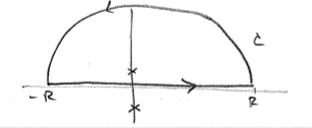
\includegraphics[width=.7\textwidth]{figures/Lec_2017_14_contour.png}
\end{center}
We will care about the limit $R\to \infty$ where the integral includes the entire real line.
Observe that the contour only encloses the pole at $z=i$. Let us integrate the function around $C$. From the residue theorem, we have
\begin{align}
  \oint_Cdz\, \frac{1}{(z+i)(z-i)} 
  = 2\pi i \text{Res}_f(i) 
  = \pi \ .
\end{align}
In the last line we have used $\text{Res}_f(i)=1/2i$. Make sure that this result is obvious---if not, take the time to check it. We can also write the integral as a sum of the real integral plus a counter-clockwise arc of radius $R$. The arc is parameterized by $z(\theta) = Re^{i\theta}$, so:
\begin{align}
  \oint_C dz\, f(z) = \int_{-R}^R dx\, f(x) 
  + \int_0^\pi iR e^{i\theta} d\theta  \, f\left(Re^{i\theta}\right) \ .
\end{align}
The first term on the right-hand side is the `ordinary' purely real integral. The second term behaves as follows:
\begin{align}
  \int_0^\pi iR e^{i\theta} d\theta  \, f\left(Re^{i\theta}\right)
  &= 
  \int_0^\pi
  \frac{Re^{i\theta}}{R^2 e^{2i\theta}+1} d\theta \ .
\end{align}
As we take the limit $R\to\infty$, the integral goes like $\sim 1/R \to 0$. Thus as long as we actually care about the integral along the entire real line, $R\to \infty$, we have
\begin{align}
  \oint_Cdz\, \frac{1}{(z+i)(z-i)}  
  = \pi 
  = \lim_{R\to\infty} \int_{-R}^R \frac{dx}{x^2+1} \ .
\end{align}
And so we find
\begin{align}
  \int_{-\infty}^\infty dx \, 
  \frac{dx}{x^2+1}
  = \pi \ .
\end{align}
This is an absolutely correct result about a \emph{real} integral that we sneakily derived without actually doing the integral. I assume one may check this by the appropriate trigonometric substitution\footnote{Just kidding, you can just check it on \emph{Mathematica}. You can even tell people that you did the trig substitution if it makes you feel better.} Observe that the critical step was that the curved part of the contour (the one that actually had imaginary parts) went to zero in a well defined limit. 
\end{example}
\begin{exercise}
What result do you get when you solve for the same integral of function $f(x)=(x^2+1)^{-1}$ over the real line, but this time you use the contour $C'$ that encircles the lower half of the complex plane?
\end{exercise}
Let's address the question of \textbf{analytic continuation}\footnote{See Appel section 5.3 for a more careful discussion.}. We started with a purely real function $f(x)$ and `generalized it' to a complex function $f(z)$ that happened to have poles in the complex plane. Because we used the residue theorem, the details of these poles (residue and whether they're enclosed by $C$) are critical for performing the integral. So a good question is: is the \emph{complex function} $f(z)$ even uniquely defined given the \emph{real} function $f(x)$?\footnote{My notation is a little glib and assumes the answer. If you want, you can write $f_\mathbbm{C}$ and $f_\mathbbm{R}$ to differentiate the two functions that are different in principle.}
\begin{center}
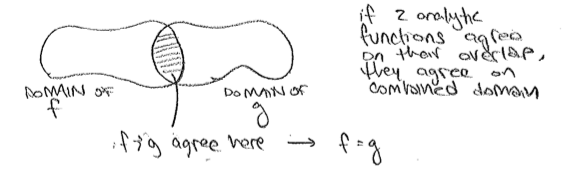
\includegraphics[width=.9\textwidth]{figures/Lec_2017_14_analytic_continuation.png}
\end{center}
There is a handy theorem that states that when two analytic functions agree on their domain of overlap, then they agree on their common domain. For \emph{meromorphic} functions, we can just imagine the domain where those singularities are not included. In our example above, $f(x)$ is analytic along the real line and $f(z)$ is a function that trivially (by construction) is analytic and matches $f(x)$ on the real line. Then the theorem says that $f(z)$ and $f(x)$ `agree' in the entire domain of analyticity; so one can \emph{analytically continue} $f(x)$ to the complex plane as long as one avoids any singularities.

The gist of the proof is that if two functions $f$ and  $g$ agree in some overlapping domain of analyticity, then their difference $h(z)\equiv f(z)-g(z)$ is also an analytic function in this domain. Analyticity means one has finite radius of convergence because it has a well defined Taylor expansion. One can then use this to argue that $h(z)$ can be defined beyond the overlapping domain. Continuity requires that $h(z)$ remains zero even outside the overlapping domain, which ensures that $f(z)=g(z)$. In other words, there is a unique analytic continuation of a function to a maximal domain of analyticity.

\begin{example}
We may naively worry about another effect. Are there some `edge' effects from the corner of the contour?
\begin{center}
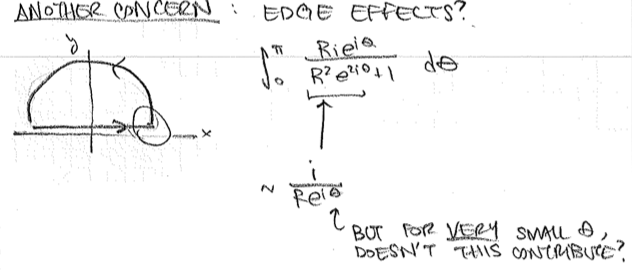
\includegraphics[width=.9\textwidth]{figures/Lec_2017_corner.png}
\end{center}
A hand-waving answer is to say that we take the $R\to\infty$ limit `first' and so that corner is pushed off into infinity. This should be totally unsatisfying since mathematical physics \emph{rarely} depends on the order in which limits are taken.  

Another response is that the integrand may be written
\begin{align}
  \frac{iR e{^i\theta}}{R^2 e^{2i\theta}+1}
  &=
  \frac{iR \left(\cos\theta + i \sin\theta\right)}{R^2(\cos2\theta + i\sin2\theta)+1}
  \\
  &=
  \frac{-R \sin\theta + iR \cos\theta}{R^2(\cos2\theta +R^{-2}) + iR^2\sin2\theta}
  % \\
  % &=
  % \frac{(-R \sin\theta + iR \cos\theta)}{R^2(\cos2\theta +R^{-2}) + iR^2\sin2\theta}
  % \\
  % &=
  % \frac{1}{R}\frac{-\sin\theta + i\cos\theta}{(\cos2\theta +R^{-2}) + i\sin2\theta}
  \\
  &=
  \frac{1}{R}
  \frac{\left(-\sin\theta + i\cos\theta\right)
  \left[(\cos2\theta +R^{-2}) - i\sin2\theta\right]
  }{(\cos2\theta +R^{-2})^2 + \sin^22\theta} \ .
\end{align}
Here it is clear that the contribution at large $R$ vanishes.
\end{example}


A more insightful answer to the above naive question is that the complex plane \emph{with infinity} is a slightly different object from the complex plane without infinity. One way to see this is to note that the complex plane can be mapped one-to-one onto a sphere. This is called \emph{stereographic projection}. The picture is this:
\begin{center}
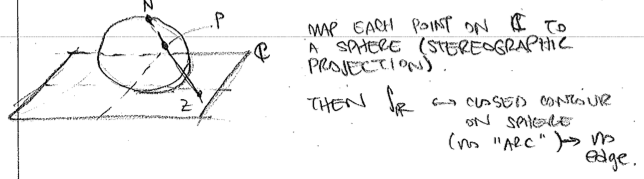
\includegraphics[width=.9\textwidth]{figures/Lec_2017_stereographic.png}
\end{center}
The idea is to place a unit sphere at the origin of $\mathbbm{C}$. The south pole of the sphere is touching $z=0$. Then for any point $z\in\mathbbm{C}$, one can draw a line from $z$ to the north pole of the sphere. There is a single unique point on the sphere that intersects that line. This maps the entire complex plane onto the sphere---except for the north pole of the sphere. We identify the north pole with complex infinity. That's right: all infinities are the same: $\infty$, $i\infty$, $\infty e^{2\pi/3}$, $-\infty$, etc. From this point of view, the real line maps onto the prime meridian of the sphere and there there are no `corners' in the contour. In fact, there's no arc component, either! The integral along the real line is a closed contour with respect to the stereographic projection. Note that the orientation of the contour depends on which hemisphere you are figuratively standing in.



\section{The Main Example: follow this carefully}
Let's try another instructive example. Here's an real integral that we would like to solve using contour integral techniques:
\begin{align}
\int dx\, f(x) = \int_{-\infty}^\infty  dx\,
\frac{2\cos x}{x^2+1} \ .
\end{align}
We can analytically continue this into a complex function by simply replacing the real variable with a complex variable, $x\to z$. This complex function $f(z)$ is analytic on the real line. The presence of simple poles at $z=\pm i$ mean that it is meromorphic with respect to the whole complex plane. It is convenient---for reasons that will be clear momentarily---to write the cosine as a sum of exponentials:
\begin{align}
  f(z) 
  = \frac{e^{iz}+e^{-iz}}{(z+i)(z-i)} 
  = \frac{e^{iz}}{(z+i)(z-i)} + \frac{e^{-iz}}{(z+i)(z-i)} 
  \equiv f_+(z) + f_-(z)
  \ .
\end{align}
With some foresight, we have separated $f(z)=f_+(z)+f_-(z)$ into two different functions.\footnote{This may seem like a not-obvious step. It is. The real reason why we're doing this is because we want to study the integrals of the separate functions $f_\pm(z)$. However, $e^{\pm ix}/(x^2+1)$ is not a purely real integral, so we packaged this as $2\cos(x)/(x^2+1)$.}

\begin{exercise}
Show that the residues of $f_\pm(z)$ at the poles $z=\pm i$ are
\begin{align}
  \text{Res}_{f_+}(i) &= \frac{1}{2ie}
  &
  \text{Res}_{f_+}(-i) &= -\frac{e}{2i}
  &
  \text{Res}_{f_-}(i) &= \frac{e}{2i}
  &
  \text{Res}_{f_-}(-i) &= -\frac{1}{2ie} \ .
\end{align}

\end{exercise}

There are now two obvious choices for convenient integration contours that include the real line with the appropriate orientation:
\begin{center}
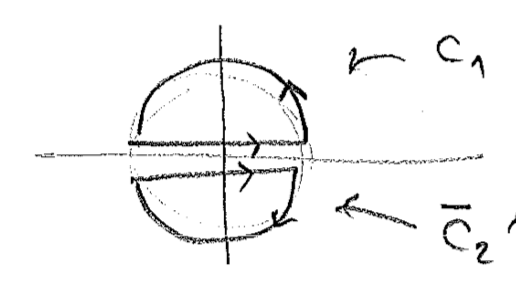
\includegraphics[width=.5\textwidth]{figures/Lec_2017_14_whichcontour.png}
\end{center}
We label the two contours are $C_1$ and $\bar C_2$. The bar over $\bar C_2$ is to remind us of the clockwise orientation; alternatively one could\footnote{This all boils down to notation. You are free to be creative with notation, but the underlying quest is \emph{clarity}. Notation doesn't change the underlying mathematics or physics, but a good notation make your ideas clearer---perhaps even to yourself.} have written $\bar C_2 = -C_2$.  Does it matter which contour we pick?

Our criteria for a convenient contour are that (1) the contour includes the real line with the appropriate orientation and (2) the rest of the contour integrates to zero. That way we can use the residue theorem:
\begin{align}
  \int_C f(z) dz 
  = \int_{-\infty}^\infty dx\, f(x)
  + \int_{\text{arc}}dz\, f(z) = 
  \int_{-\infty}^\infty dx\, f(x)
  = \sum_{i=\text{poles}}\text{Res}_f(z_i) \ ,
\end{align}
where we recall that $i$ is runs over the poles enclosed by the contour $C$. The condition that the integral over the arc vanishes determines which contour we take.
% We may conveniently parameterize the arcs as follows:
% \begin{align}
%   z(\theta) &= R\cos\theta + i R\sin\theta
%   \label{eq:z:paramterization:large:arc}
% \end{align}
% where for $C_1$ the arc is given by $\theta \in [0,\pi]$ while for $\bar C_2$ the arc is $\theta\in[0,-\pi]$. 
We assume the limit $R\to \infty$. The arc integrals are then:
\begin{align}
  \int_{\text{arc}}
  dz \, 
  %  \left[f_+(z) + f_-(z)\right]
  f_\pm(z)
  =
  \int_\text{arc}
  Re^{i\theta}
  d\theta \, 
  \frac{e^{\pm iz(\theta)}}{z(\theta)^2+1}
  % + 
  % \int_\text{arc}
  % d\theta \, 
  % \frac{e^{iz}}{z^2+1} 
  \ .
\end{align}
% When we plug in the parameterization \eqref{eq:z:paramterization:large:arc}, we see that 
The denominator of $f_\pm$ scales like $R^2$. There's an additional factor of $R$ in the numerator coming from $dz$, and so it may  appear that \emph{either} $C_1$ or $\bar C_2$ could be used. However, recall that $f_{\pm}(z)\sim e^{\pm iz}$ and exponentials beat polynomials. Plugging in $z = R(\cos\theta + i \sin\theta)$ into the exponentials gives
\begin{align}
  e^{\pm iz} &= e^{\pm i\left(R\cos\theta + i R\sin\theta\right)} \ .
\end{align}
Make sure you understand \emph{why} we chose to plug in $z = R(\cos\theta + i \sin\theta)$ into the exponential rather than $z = Re^{i\theta}$. If you're confused, pay special attention to the next step. The difference between $C_1$ and $\bar C_2$ is the range (and direction) of $\theta$. 
\begin{itemize}
  \item $C_1$ lives in the upper half plane so the imaginary part of $z$ is positive: $R\sin\theta > 0$ \ .
  \item $C_2$ lives in the lower half plane so the imaginary part of $z$ is negative: $R\sin\theta < 0$\ .  
\end{itemize}
This makes it easy to read off the convergence properties of the exponential
\begin{align}
  e^{\pm iz} &= (\text{oscillating})e^{\mp R\sin\theta} \ .
\end{align}
The oscillating part is not relevant: since $|e^{i\varphi}| = 1$ , this factor doesn't actually affect the magnitude of the contribution of the integrand, just the phase. The $\exp(\mp R\sin\theta)$ factor, on the other hand, is everything. 
\begin{itemize}
  \item $e^{- R\sin\theta}$ is exponentially suppressed when $\sin\theta > 0$, this corresponds to the upper half plane and so we use the $C_1$ arc to complete the integration contour of the $f_+(z)\sim \exp(-R\sin\theta)$ integrand.
  \item $e^{+ R\sin\theta}$ is exponentially suppressed when $\sin\theta < 0$, this corresponds to the lower half plane and so we use the $\bar C_2$ arc to complete the integration contour of the $f_-(z)\sim \exp(+R\sin\theta)$ integrand.
\end{itemize}
Because the $e^{-R}$ exponential suppression defeats the polynomial $R^{-1}$ scaling, the vanishing of the integral along the arc is determined only by this exponential factor: $\lim_{R\to\infty}e^{-R}/R\to 0$. We thus have the following approach to the original real integral:
\begin{align}
  \int dx\, f(x) &= \int_{-\infty}^\infty  dx\,
\frac{2\cos x}{x^2+1} 
  = 
  \int_{-\infty}^\infty  dx\,
  \frac{e^{+ix}}{x^2+1} 
  +
  \int_{-\infty}^\infty  dx\,
  \frac{e^{-ix}}{x^2+1} 
  \\ 
  &=
  \int_{C_1} dz\, 
  \frac{e^{+iz}}{z^2+1} 
  +
  \int_{\bar C_2} dz\, 
  \frac{e^{-iz}}{z^2+1} 
  \\
  &=
  2\pi i \text{Res}_{f_+}(i)
  -
  2\pi i \text{Res}_{f_-}(-i)
\ .
\end{align}
In the second step we have used the fact that the integral along the real line can be extended by large arcs along $C_1$ or $\bar C_2$ as long as the integral along those arcs vanishes. The residues are straightforward: 
\begin{align}
  \text{Res}_{f_\pm}(\pm i) = \pm \frac{1}{2ie}
\end{align}
so that the final result is
\begin{align}
  \int_{-\infty}^\infty dx\, f(x) &= \frac{2\pi}{e} \ .
\end{align}

\section{A fancy example}

 Here's an example of the residue theorem used to calculate an integral along just the positive real line,
 \begin{align}
  \int_0^\infty dx\, x^{1/3} F(x) \ .
 \end{align}
 We can trivially analytically continue the integrand by replacing $x\to z$. Let us assume that $F(x)$ is a meromorphic function with poles away from the positive real line. Let us further assume further that $F(z)$ is sufficiently suppressed for $|z| = R \gg 1$. What does `sufficiently suppressed' mean? We will discover that the residue theorem is useful as long as $F(z) \sim R^{-n}$ with $n>4/3$. 

\begin{exercise}
Through the discussion of this example, please keep two questions in mind:
\begin{enumerate}
  \item What happens if $F(x)$ is analytic everywhere, not just meromorphic? More specifically, what happens if $F(x)$ has no simple poles anywhere?
  \item Why do we need $F\left(Re^{i\theta}\right)$ to decay faster than $R^{-4/3}$ for large $R$?
\end{enumerate}
Eventually the answers will be clear. See if you can discover them before we say it explicitly.
\end{exercise}
  
  The $x^{1/3} \to z^{1/3}$ factor is tricky. It tells us that there's an \emph{branch cut} in our integrand: if we start at some point and went a full circle around the origin, say $z(\theta) = e^{i\theta}$ for $\theta\in[0,2\pi]$, then $z^{1/3}$ doesn't return to the origin. This means you probably need to extend the complex plane into Riemann sheets. Practically what this means is that we have to pick a branch cut that prevents us from taking contours that are `full circles' around the origin. We have the freedom to pick the orientation of this branch cut, but in this case it is convenient to pick it along the positive real line\footnote{If you want to be careful to make sure that you're not interfering with the original integral, you can put the branch cut just below the real line by some vanishingly small amount and take that amount to zero at the end of the calculation.}. Let's take a peculiar contour that includes the integration region we want, $x\in [0,\infty)$, then circles the entire complex plane, and returns back to zero along $x\in (\infty, 0]$. 
 \begin{center}
 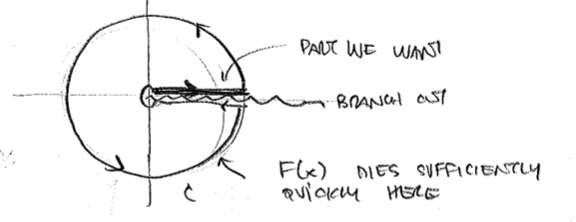
\includegraphics[width=.8\textwidth]{figures/Lec_2017_14_branch.png}
 \end{center}
 In the past, we'd have said that the integral along $x\in [0, \infty)$ should cancel that from $x\in (\infty, 0]$. However, we now notice that there's a branch cut separating those two regions. Indeed, you may already see that the \emph{integrand} is not identical along those two lines. 

Construct the following contour integral:
 \begin{align}
  \oint_C  dz\, z^{1/3} F(z) &= 
  \int_0^\infty dx \,  x^{1/3}F(x)
  + \int_{\text{arc}} dz \, z^{1/3} F(z)
  + \int_\infty^0 dx \left(x e^{2\pi i}\right)^{1/3} F\left(e^{2\pi i} x\right) \ .
 \end{align}
 The left-hand side is simple to evaluate with the residue theorem and will depend on the poles of the unspecified function $F(z)$. On the right-hand side, the integral along the arc vanishes by the assumptions we've made about $F(z)$ becoming exponentially small for large arguments, $|z|=R\gg 1$.  Finally, we notice that the third term on the right-hand side we've written $z=xe^{2\pi i}$; this is critical since it includes the phase that $z$ picks up when traversing the large circular path. Since $F(z)$ is meromorphic, we may simply replace $F(x\exp(2\pi i)) \to F(x)$. However, the $z^{1/3}$ needs some care. Writing $f(z)\equiv z^{1/3}F(z)$, We find:
 \begin{align}
  2\pi i \sum_{j=\text{poles}}  \text{Res}_{f(z)}(z_j)
  =
  \left(1-e^{2\pi i/3}\right) \int_0^\infty dx\,  x^{1/3} F(x) \ .
 \end{align}
The $-e^{2\pi i/3}$ came from the $1/3$-power of the phase. The minus sign comes from $\int_{\infty}^0 dx = -\int_0^\infty dx$. At this point, we have
\begin{align}
  \int_0^\infty dx \, x^{1/3}F(x)
  &= 
  \left(1-e^{2\pi i/3} \right)^{-1}
  2\pi i \sum_{j=\text{poles}}  \text{Res}_{f(z)}(z_j) \ .
\end{align}
Two important notes:
\begin{enumerate}
  \item We are taking the residue of $z^{1/3}F(z)$ at $z_j$. Don't forget the $z^{1/3}$ part of the function.
  \item The result is not obviously real, even though the integral is supposed to be real. 
\end{enumerate}
\begin{exercise}
Choose a function $F(x)$ that satisfies the requirements to use the residue theorem to integrate $\int_0^\infty dx\; x^{1/3}F(x)$. Show that the residue theorem gives a real result. Double check the result in \emph{Mathematica} or \emph{SciPy}.
\end{exercise}
\begin{exercise}
Check the result for $F(x) = e^{-x}/(x^2+1)$. Does it work? If not, why not?
\end{exercise}

\begin{example} \textbf{Unparticles.}
Here's an actual example from something called \emph{unparticle physics}\footnote{\url{https://arxiv.org/abs/hep-ph/0703260}}. In 2006 Howard Georgi proposed that rather than particles with unique masses, a theory could have states with a continuum of masses so that the theory is scale-invariant. Perhaps in part due to its silly name, the unparticle idea has largely been subsumed into the study of conformal dynamics using tools like the \acro{AdS/CFT} correspondence.

The momentum-space Green's function for a particle of mass $m$ takes the form
\begin{align}
  \tilde G(p) = \frac{1}{p^2 - m^2 + i\varepsilon} \ ,
\end{align}
where here $p^2$ is the four-momentum squared and $m^2$ is the mass of the particle. In the next section you will recognize this as the Green's function for a harmonic oscillator $p^2$ replaced by the angular frequency $\omega^2$ and $m^2$ replaced by the resonant angular frequency $\omega_0^2$. A scale-invariant `unparticle' is characterized by its scaling dimension $d$ and has a Green's function that is an integral over the possible masses:
\begin{align}
  \tilde G(p) &= \int_0^{\infty} d\mu^2
  \frac{(\mu^2)^{d-2}}{p^2 - \mu^2 + i\varepsilon}
  \ .
\end{align}
We can perform this integral using the residue theorem with some modest assumptions about $d$ to ensure convergence. In general, $d$ is non-integer and therefore this integral has a branch cut. For convenience, we take the branch cut just below the positive real axis.  We observe that the integration variable is $z \equiv \mu^2$. There is a simple pole at $z = p^2+i\varepsilon$; owing to the $+i\varepsilon$ it is formally off of the cut. The significance of this $i\varepsilon$ is addressed below, but for now we may take $\varepsilon\to 0$ once we are convinced that the pole is formally separated from any cuts or contours.

The residue theorem tells us that
\begin{align}
  \oint_\text{pacman} {dz} \frac{-z^{d-2}}{z-(p^2+i\varepsilon)}
  &=
  \left(1-e^{2\pi i(d-2)}\right) \tilde G(p) \ ,
\end{align}
where we assume that $d < 2$ so that the integrals along the arc converge to zero. The residue at $z=p^2$ is 
\begin{align}
  \text{Res}_f(p^2) =& -(p^2)^{d-2} 
  &
  f(z)\equiv 
  \frac{-z^{d-2}}{z-p^2} \ .
\end{align}
Applying the residue theorem to perform the contour integral then gives us
\begin{align}
  \tilde G(p) &= \left(1-e^{2\pi i(d-2)}\right)^{-1} (2\pi i) (-) (p^2)^{d-2}  \ .
\end{align}
We would like to turn that prefactor into a sine. To do this, we write
\begin{align}
  1-e^{2\pi i(d-2)}
  =
  e^{\pi i(d-2)}\left(e^{-\pi i(d-2)}-e^{\pi i(d-2)}\right)
  = -2i e^{\pi i(d-2)} \sin(\pi d) \ .
\end{align}
We used $e^{\pm\pi i(d-2)} = e^{\pm\pi id}$. Plugging this into $\tilde G(p)$ gives
\begin{align}
  \tilde G(p) &= 
  \frac{\pi}{\sin(\pi d)}
  e^{i\pi (d-2)}
  (p^2)^{d-2}
  \\
  & =
  \frac{\pi}{\sin(\pi d)} (-p^2)^{d-2} \ .
\end{align}
Note the key step where an overall complex phase $e^{\pi i(d-2)}$ is absorbed into the $(p^2)^{d-2}$ factor as a sign.
\end{example}

We won't worry too much about branch cuts in this course. However, they do occasionally show up in physical manifestations, such as in dispersion relations\footnote{See, e.g., \url{https://arxiv.org/abs/1610.06090} for a peek at how it can show up in quantum field theory.}.

\part{Everything is a Harmonic Oscillator}

\chapter{The Harmonic Oscillator}

\section{The most familiar problem in physics}
% \lecdate{lec~12} 

We return to the problem of solving for Green's functions. Our favorite example---arguably, the \emph{only} example\footnote{Upon generalizing to higher dimensions, curvilinear coordinates... most everything is a harmonic oscillator. Physicists have Harmonic Oscillators in different area codes.}---is the harmonic oscillator. The differential operator is
\begin{align}
  \mathcal O = \left(\frac{d}{dt}\right)^2 + \omega_0^2 \ .
  \label{eq:O:HO}
\end{align}
\begin{example}
The equation of motion for a harmonic oscillator with spring constant $k$ and displacement $f(t)$ from equilibrium is simply the equation $F=m\ddot{f} = -k f(x)$. We have defined $\omega_0^2 = k/m$.
\end{example}
\begin{exercise}
Compare our definition of $\omega_0^2 = k/m$ to what you remember the resonant frequency of an ideal spring to be. What---you do not remember? That is okay, physicists do not have to remember these details: we can re-derive them. What---you do not have time to rederive this? Okay, use dimensional analysis. 
\end{exercise}
\begin{exercise}
One may argue that the harmonic oscillator operator should be defined with an overall minus sign. Life is too short to quibble over signs in these notes. Please confirm that if  $\mathcal O_\text{minus} = -\mathcal O$, then the Green's function is simply $G_\text{minus} = - G$. Relate this to the physical interpretation of the Green's function equation. {Hint:} if you pluck a guitar string in the opposite direction, you still get a `unit' wave.
\end{exercise}
The Green's function equation tells us that the Green's function $G(t,t_0)$ is the spring `response' at time $t$ to a `unit displacement' at $t_0$:
\begin{align}
  G''(t,t_0) + \omega_0^2 G(t,t_0) = \delta(t-t_0) \ .
  \label{eq:HO:Greens:eqn}
\end{align}
Recall that the arguments $t$ and $t_0$ are analogous to the indices of a finite-dimensional matrix. We are primarily concerned about the $t$-dependence of $G(t,t_0)$.  For notational convenience, we will set $t_0=0$ and not list it explicitly. What this means is that we are choosing a `zero' for how we measure time: $t=0$ corresponds to the moment of the `unit displacement' source. Positive times correspond to times after the unit displacement. Negative times correspond to times before the unit displacement.

\begin{exercise}
Our system and the laws of physics in this model are time translation invariant. It does not matter where we pick the zero of time. This tells us that we can always make the replacement $t\to t-t_0$ to recover the source time. In other words, as long as the system is invariant along translations of the coordinates $x$, we have $G(x,y) = G(x-y)$. Convince yourself that this is true. Consider what kinds of scenarios would break this relation.
\end{exercise}

\section{Fourier Transform}

The first thing to do is to write $G(t,t_0)$ as a Fourier transform with respect to $t$. Please refer to Appendix~\ref{app:Fourier} for our set of Fourier transform conventions. We can write $G(t)$ as an integral over Fourier modes with frequency $\omega$ and weight (Fourier transform) $\tilde G(\omega)$:
\begin{align}
  G(t) &= \int_{-\infty}^\infty\dbar \omega \, e^{-i\omega t} \tilde G(\omega) 
  &
  \dbar = \frac{d}{2\pi}
  \ .
  \label{eq:HO:Greens:Fourier}
\end{align}
We say that $\tilde G(\omega)$ is the Fourier transform of $G(t)$. The key point is that the $t$-dependence of $G(t)$ has been sequestered into the $e^{-i\omega t}$ plane waves. This is convenient since these plane waves are eigenfunctions of the derivative operator:
\begin{align}
  \frac{d}{dt} e^{-i\omega t} &= -i\omega e^{-i\omega t} \ .
\end{align}
The left-hand side of the Green's function equation \eqref{eq:HO:Greens:eqn} is
\begin{align}
  \mathcal O_t G(t,t_0) 
  &= 
  -
  \int_{-\infty}^\infty \dbar \omega \, 
  \left(\omega^2-\omega_0^2\right) e^{-i\omega t} \tilde G(\omega,t_0) \ .
\end{align}
The right-hand side is simply the Fourier transform of $\delta(t-t_0)$:
\begin{align}
  \delta(t-t_0)
  &=
  \int_{-\infty}^\infty \dbar \omega \, e^{-i\omega (t-t_0)} \ .
  \label{eq:delta:fourier}
\end{align}
\begin{exercise}
Use our conventions for the Fourier transform \eqref{eq:HO:Greens:Fourier} (see also Appendix~\ref{app:Fourier}) to confirm the Fourier representation of $\delta(t-t_0)$ in \eqref{eq:delta:fourier}. In our notation, the Fourier coefficients $\tilde f(\omega)$ of a function $f(t)$ is
\begin{align}
  \tilde f(\omega) &= 
  % \frac{1}{2\pi}
  \int_{-\infty}^\infty d t\, e^{i\omega t} f(t) \ .
\end{align}
\end{exercise}
So the Green's function equation for the 1D harmonic oscillator, \eqref{eq:HO:Greens:eqn}, tells us
\begin{align}
  -
  \int_{-\infty}^\infty \dbar \omega \, 
  \left(\omega^2-\omega_0^2\right) e^{-i\omega t} \tilde G(\omega)
  &=
  \int_{-\infty}^\infty \dbar \omega \, e^{-i\omega t}
  \ .
  \label{eq:G:HO:Fourier:equation:integrals}
\end{align}
For simplicity we have set $t_0=0$ and don't write it explicitly. There's a rather unscrupulous\footnote{I don't think this is rigorously valid, but the result is true. The ends don't justify the means, but let's take this morally ambiguous shortcut to make the big picture clear. I encourage you to live the rest of your lives with virtue.} way to solve this equation for $\tilde G(\omega)$. Since the two sides of this expression are equal, they have the same Fourier expansion. This implies that the Fourier coefficients are equal. Since both sides are already written as Fourier expansions, we can just match the coefficients of the basis functions, $e^{-i\omega t}$. This gives us:
\begin{align}
  \tilde G(\omega) &= \frac{-1}{\omega^2-\omega_0^2}
  \label{eq:G:HO:Fourier:term}
\end{align}
\begin{exercise}
Prove \eqref{eq:G:HO:Fourier:term} honestly. {Hint}: Start with \eqref{eq:G:HO:Fourier:equation:integrals} and project out the Fourier coefficients. Recall that you do this by taking the inner product with one of the basis functions and then using the orthogonality of the eigenbasis. You may need to be careful with the normalization.
\end{exercise}
\begin{exercise}
In \eqref{eq:G:HO:Fourier:equation:integrals} we had already set $t_0 = 0$. What is the expression for $\tilde G(\omega)$ if we kept $t_0$ explicit?
\label{eq:ex:Gtilde:with:t0:explicit}
\end{exercise}
That was the critical step: we have successfully solved for the Green's function Fourier coefficient. This means that we have a closed form expression for the Green's function by plugging $\tilde G(\omega)$ into \eqref{eq:HO:Greens:Fourier}:
\begin{align}
  G(t) &=  \int_{-\infty}^\infty \dbar \omega
  \, 
  \frac{-e^{-i\omega t}}{\omega^2-\omega_0^2} \ .
  \label{eq:G:HO:Fourier:Rep:t0:0}
\end{align}
All that's left is for us to actually \emph{do} this integral. Fortunately, this integral should look very similar. It seems to beg for us to solve using the residue theorem. 
\begin{exercise}
What are the poles of the integrand in \eqref{eq:G:HO:Fourier:Rep:t0:0}? What are their associated residues? What is the residue if $t_0\neq 0$?
\end{exercise}

\subsection{Contour Integral}

The integral \eqref{eq:G:HO:Fourier:Rep:t0:0} looks like it's perfect for contour integration. There's an exponential factor on top that will determine the convergence, and the denominator can be factored to see where the poles are. Except we notice something troubling:
\begin{align}
  \frac{-e^{-i\omega t}}{\omega^2-\omega_0^2} 
  &=
  \frac{-e^{-i\omega t}}{(\omega - \omega_0)(\omega + \omega_0)} \ .
  \label{eq:HO:integrand:real:pole}
\end{align}
The poles are located at $\omega = \pm \omega_0$. These are \emph{on the real axis}, precisely along the integration contour! How annoying!

Now you may want to have an existential moment. Remind yourself that all we're doing is solving for the behavior of the one-dimensional \emph{harmonic oscillator}. This is an eminently \emph{physical} system. We could have written this system as $\mathcal O f(t) = s(t)$ where $f(t)$ is the displacement of a harmonic oscillator and $s(t)$ is some driving function. The Green's function, $G(t,t_0)$ gives the response of the system to a `unit' driving function, $s(t) = \delta(t-t_0)$. The response of the system should be perfectly physical. And yet---\emph{and yet}---we now face an integral \eqref{eq:G:HO:Fourier:Rep:t0:0} that seems to run right into not only one, but \emph{two} singularities along the integration contour!
\begin{center}
\includegraphics[width=.4\textwidth]{figures/Lec_2017_16_HO_Poles.pdf}
\end{center}
Please do take a brief moment to ponder at this existential crisis. This is an apparent failure of our theory---our calculation hits a pole, you get an infinity, and it's not clear what's going on. Rather than anguish, though, we should see if our theory is trying to tell us something. 

In order to figure out what's going on, let's do something wild. The poles on the real axis are in the way. Let's just move them out of the way by giving them small imaginary parts. Each pole can either be pushed above or below the real line:
\begin{center}
\includegraphics[width=.4\textwidth]{figures/Lec_2017_16_HO_PoleShift.png}
\end{center}
To be clear: are \emph{changing} the integral.\footnote{I have altered the poles. Pray that I do not alter them further.} We are exploring what happens when the expression \eqref{eq:G:HO:Fourier:Rep:t0:0} is changed, as if the poles were slightly complex the whole time. In other words, we are \emph{changing} the original differential operator, \eqref{eq:O:HO}. We're not yet motivating \emph{why} we want to do this; we'll justify it post-facto. For now, let's just be happy that our contours no longer bump into the poles. 

\section{Going under the poles?}
Let's try going under the poles, that is: let's push the poles into the upper half-plane with small imaginary parts:
\begin{center}
\includegraphics[width=.6\textwidth]{figures/Lec_2017_16_underpole.png}
\end{center}
This means that we have deformed the integrand \eqref{eq:HO:integrand:real:pole}:
\begin{align}
\frac{-e^{-i\omega t}}{(\omega - \omega_0)(\omega + \omega_0)}
&\to
\frac{-e^{-i\omega t}}{(\omega - \omega_0 - i\varepsilon)(\omega + \omega_0 - i\varepsilon)} \ .
\label{eq:HO:integrand:upper:poles}
\end{align}
To make it clear that we are treating $\omega$ as a complexified variable, let's write it as $z$:
\begin{align}
  \omega \to z \ .
 \end{align}
Now let's go through the exercise of performing the integral along the real line by using the residue theorem. To do this have to choose a contour that includes the real line. We have two options, $C_+$ and $\bar C_-$, where the bar reminds us of the orientation:
\begin{center}
\includegraphics[width=.6\textwidth]{figures/Lec_2017_16_pokeup.pdf}
\end{center}
Which contour do we pick? Does it matter? (Yes!) The contours differ by whether the `large arc' has positive or negative real part. We can parameterize these arcs with respect to their real and imaginary parts:
\begin{align}
  z(\theta) &= R\cos\theta + i R\sin\theta \ ,
\end{align}
where for $C_+$ the arc is given by $\theta \in [0,\pi]$ while for $\bar C_-$ the arc is $\theta\in[0,-\pi]$. Note that the \emph{orientation} matters here---the $\bar C_-$ arc is moving in the clockwise direction.\footnote{Do people reading this even know why it is called `clockwise'? Analog clocks had mechanical arms that rotate.} The component in the imaginary axis is determined by $R\sin\theta$. Because $R$ is real and greater than zero, we have
\begin{align}
  \text{for $C_+$:}\, \sin\theta &> 0
  &
  \text{for $\bar C_-$:}\, \sin\theta &<0 \ .
  \label{eq:HO:which:contour}
\end{align}
%
How do we pick a contour? The criteria for completing the real line into a contour is that the integral along the contour vanishes, that way
\begin{align}
  \oint_C dz\, f(z) 
  = \int_{-\infty}^\infty dx\, f(x) + \lim_{R\to \infty} R \int_\text{arc} d\theta f(Re^{i\theta}) 
  = \int_{-\infty}^\infty dx\, f(x) \ .
\end{align}
And hence one can use the residue theorem to solve the contour integral on the left-hand side and relate it to the real integral on the right-hand side\footnote{I say `real integral' but of course the integrand \eqref{eq:HO:integrand:upper:poles} is now a complex quantity. The point is that we  only integrating along the real line.}. 
%
So which contour satisfies
\begin{align}
  \lim_{R\to \infty} R \int_\text{arc} d\theta 
  % f(Re^{i\theta})  
  \frac{-e^{-i(R\cos\theta + iR\sin\theta) t}}{(Re^{i\theta} - \omega_0 - i\varepsilon)(Re^{i\theta} + \omega_0 - i\varepsilon)}
  \to 0 \ ?
\end{align}
I was a little slick and chose to write $z = R\cos\theta + iR\sin\theta$ in the numerator while writing the more compact $z=Re^{i\theta}$ in the denominator. The convergence\footnote{I tend to say convergence, what I really mean is `vanishes as $R\to \infty$.'} of the integrand depends on the exponential factor in the numerator:
\begin{align}
  e^{-i(R\cos\theta + iR\sin\theta) t} = 
  e^{-iRt\cos\theta} e^{Rt\sin\theta} \ .
\end{align}
The first factor is purely oscillatory and is $\mathcal O(1)$ as $R\to\infty$. The second factor is either exponentially decaying or exponentially growing with large $R$. Convergence depends specifically on this second factor, $e^{-Rt\sin\theta}$. Since $R>0$, this depends on two things: the sign of $\sin\theta$ and the sign of $t$. The integral along the arc vanishes in the $R\to\infty$ limit when:
\begin{align}
  t > 0 \quad\text{and}\quad \sin\theta < 0 &
  &\text{or}&&
  t < 0 \quad\text{and}\quad \sin\theta > 0 \ .
  \label{eq:t:gtr:less:upper:poles}
\end{align}
Or in other words:
\begin{align}
  t>0 &\to \bar C_{-} 
  &
  t<0 &\to C_+ \ .
  \label{eq:t:sign:contour:HO}
\end{align}
% \begin{itemize}
%   \item $t>0$ and $\sin\theta > 0$ or
%   \item $t<0$ and $\sin\theta < 0$ \ .
% \end{itemize}
Recall that we have set $t_0 = 0$; if you did Exercise~\ref{eq:ex:Gtilde:with:t0:explicit}, you would know that restoring $t_0$ corresponds to $t\to t-t_0$ in the conditions above.

The Green's function equation \eqref{eq:Greens:func:as:inverse} is simply that $$\mathcal O_t G(t,t_0) = \delta(t-t_-)\ .$$ This tells us that the Green's function $G(t,t_0)$ is the \emph{response} measured at time $t$ to a $\delta$-function source at $t_0$. Thus the sign of $t-t_0$ corresponds to whether we are measuring the response \emph{before} or \emph{after} the cause. If you are like me, your eyes just lit up with joy. Something very exciting has happened: in this odd discussion about pushing around the poles of $\tilde G$, we have found that we were secretly talking about \emph{causality}.  

Before we progress, let's be clear: we expect that effects happen \emph{after} causes. This means that physical dynamics obey $t-t_0 >0$. A nice theory would tell us that you cannot have an effect before a cause. At the beginning of this course, we talked about locality as one of the motivating factors for why physical dynamics are described by differential operators. This was closely tied to the idea of causality, since non-local effects with spacelike separation can be non-causal in some reference frame. Perhaps amusingly---but beyond the scope of this course or my expertise---the notion of causality and locality in fundamental theories of nature continues to be a theme in cutting edge theoretical research. 

\paragraph{Causal propagation.}
For the specific case of $t>0$ (or $t-t_0>0$ if we restore $t_0$), we observe from \eqref{eq:t:gtr:less:upper:poles} that the integral \eqref{eq:HO:integrand:upper:poles} converges when $\sin\theta <0$. In other words, for times \emph{after} the initial cause at $t_0=0$, the appropriate contour is $\bar C_-$. 
\begin{exercise}
What is the value of the contour integral 
\begin{align}
  \oint_{\bar{C}_-} dz\, \frac{-e^{-i z t}}{(z - \omega_0 - i\varepsilon)(z + \omega_0 - i\varepsilon)} \ ?
\end{align}
Hint: you shouldn't have to do any work.
\end{exercise}
% The contour integral above vanishes along the arc when $t>0$, so it is the correct contour when doing the Fourier transform to get $G(t)$ from $\tilde G(\omega)$. However, 
This contour encloses no poles. No poles means no residues. This means that the contour integral vanishes and the Fourier transform vanishes. In other words, 
\begin{align}
  G(t>0) &= 0 \ .
  \label{eq:HO:G:t:gtr:0:zero}
\end{align}

\begin{example}
The statement that $G(t>0)=0$ should make you sad and possibly upset. This means that there is \emph{no} effect that happens after some cause at $t_0=0$.
\end{example}

\paragraph{Acausal propagation.} By now you see the writing on the wall. Something perverse has happened: after a $\delta$-function disturbance, information is not traveling forward in time because $G(t)=0$ for $t>0$. This, in turn, was self-evident in because for $t>0$, we were required to take the $\bar C_-$ contour in order that the contribution of the arc vanishes. At this point, you must feel the dread of what's coming next. If we take the $t<0$ case in \eqref{eq:t:gtr:less:upper:poles}, we are forced to take the $C_+$ contour. This contour indeed picks up poles and so we expect it to be non-zero. Thus we find that $G(t<0) \neq 0$, which is awful because this $t<0$ corresponds to an \emph{effect that happens before the cause}. 

\begin{exercise}
Taking $t_0=0$ for simplicity, show that the exact result for the acausal Green's function is
\begin{align}
  G(t<0) &= \frac{-1}{\omega_0}\sin\omega_0t \ .
  \label{eq:HO:G:t:less:0:nonzero}
\end{align}
Hint: the relevant residues are $\pm e^{\pm i\omega_0t}/2\omega_0$ \ .
\end{exercise}
You should \emph{do} the above exercise as practice for the main contour integral of this entire course. If you are stuck, you can keep reading these notes.\footnote{By now you should know that learning physics requires \emph{doing} physics. Reading/watching someone else do physics is one of the least efficient ways of improving yourself.} 

To help you along, let me even set up the integral for you. We start with $G(t)$ in \eqref{eq:HO:integrand:real:pole}, where we rewrote the integrand in \eqref{eq:G:HO:Fourier:Rep:t0:0} to make the pole structure clear. We then said that we wanted to push the poles off the real line. This \emph{changes} the physical problem, but we'll worry about what that means later. In this case, we move the poles into the upper half-plane so that each pole has a small imaginary part. The poles are then located at $\pm \omega_0 + i \varepsilon$. The resulting integral is:
\begin{align}
  G(t) &= 
  \int_{-\infty}^\infty \frac{d\omega}{2\pi} 
  \frac{-e^{-i\omega t}}{(\omega - \omega_0-i\varepsilon)(\omega + \omega_0-i\varepsilon)} 
  \ .
\end{align}
Complete the real integral into a contour integral; we'll re-label our variables to remind us that we're in the complex plane, $\omega\to z$. The contour that we select, $C_+$, came from the $e^{-i\omega t}$ factor. The result is:
\begin{align}
  \oint_{C_+}
  \frac{dz}{2\pi} 
  \frac{-e^{-iz t}}{(z - \omega_0-i\varepsilon)(z + \omega_0-i\varepsilon)}
  =&\phantom{+} 
  \int_{-\infty}^\infty \frac{d\omega}{2\pi} 
  \frac{-e^{-i\omega t}}{(\omega - \omega_0-i\varepsilon)(\omega + \omega_0-i\varepsilon)} 
  \nonumber
  \\
  &
  + 
  \cancel{
  \lim_{R\to\infty} \int_{0}^\pi \frac{Rd\theta}{2\pi} 
  \frac{-e^{-i(R\cos\theta + i R\sin\theta)t}}{(Re^{i\theta} - \omega_0-i\varepsilon)(Re^{i\theta} + \omega_0-i\varepsilon)} 
  }
  \label{eq:HO:G:integral:adv:1}
  \\
  &=
  2\pi i \sum_{z_\pm=\pm\omega_0+i\varepsilon} \text{Res}_f(z) \ ,
  \label{eq:HO:G:integral:adv:2}
\end{align}
where $f$ is understood to be the integrand. 
%
From here you should be able to read off the result. Confirm that we can take the $\varepsilon\to 0$ limit; this tiny shift was only there to tell us that the poles live in the upper half-plane.

\paragraph{Advanced propagator.}
The causal ($t>0$) and acausal ($t<0$) cases in \eqref{eq:HO:G:t:less:0:nonzero} and \eqref{eq:HO:G:t:gtr:0:zero} respectively may be combined into a single expression:
\begin{align}
  G_\text{adv}(t) &= \frac{-1}{\omega_0}\sin(\omega_0t) \Theta(-t) \ ,
  \label{eq:HO:G:adv:theta}
\end{align}
where we use the Heaviside step function
\begin{align}
  \Theta(x) = 
  \begin{cases}
  1 & \text{if}\; x>0\\
  0 & \text{if}\; x<0 \ .
  \end{cases}
  \label{eq:Heaviside:Theta}
\end{align}
\begin{exercise}
Check the overall sign. I keep screwing this up. You are henceforth responsible for the overall sign and I absolve myself of any mistakes due to this sign.
\end{exercise}
This is the \textbf{advanced} propagator. Even though `advanced' is often a positive adjective when applied to your progress\footnote{I once read a story about a particle physicist who started a conversation with a stranger on the plane. The stranger explains, ``My son is really quite brilliant. He's studying physics at an Ivy league university.'' The physicist says, ``Oh, how nice. You know, I'm a physicist.''  The stranger then asks what kind of physics, to which the physicist says ``I study elementary particles.'' The stranger responds with, ``Ah yes. Well, my son studies advanced particles.'' I no longer remember where I read this story, but I can attest to meeting people like this.} In this context, however, `advanced' is a \emph{bad} word. It means \emph{acausal}: the cause comes \emph{after} the effect. This does not make any sense, and we reject this as non-sense. 

After an appropriate amount of indignant disdain, we can reflect on how the heck we got here\footnote{If your response is \emph{Christmas! Christmas eve last year}, then I applaud your taste in musical theater.}. We make two observations:
\begin{enumerate}
\item After checking all of our work, the main conclusion from this non-sense result is that our approach of pushing the poles \emph{up} into the upper half-plane must have been wrong. We see that the position of the poles tells us about the causality of the system. By pushing the poles off the real axis, we have imposed a sense of causality in time. We should see what happens when we push the poles \emph{down} into the lower half-plane. 

\item Even though the \emph{physics} of advanced propagator is utter rubbish because it breaks causality, we also appreciate that it is a perfectly reasonable \emph{mathematical} solution. The harmonic oscillator dynamics encoded in our differential operator $\mathcal O_t$ is symmetric with respect to time-reversal symmetry\footnote{The behavior of our models under $t\to -t$ is a powerful diagnostic for understanding our physical theories. One of my friends was in a pub the night before lecture and some of the pub regulars, who knew he was a physicists, asked him what he was lecturing on the next day. He said he was going to talk about reversing the direction of time, to which they cautiously responded: `\emph{... we can do that??}'}. The `physical' interpretation is analogous to seeing a bunch of ripples starting at the edges of a pond that move inward until they reach a singularity ($\delta$-function!?) at which point the pond spits out a small pebble. 
\end{enumerate}


\begin{exercise}
At this point, you should be able to solve the case of the causal Green's function without any additional guidance. In fact, without doing any work, you should see that by pushing the poles down into the lower half plane, the propagator will be causal. With a little bit of thought, you may be able to write the analog of \eqref{eq:HO:G:adv:theta}, the retarded Green's function,
%\footnote{In the same way that `advanced' means something different colloquially versus for physics, we use this word very carefully. One of my friends in graduate school was an international student who liked to make physics puns. At some point she playfully admonished late arriving undergraduates for being `retarded,' which required quite a bit of care to clarify the situation to everyone involved.}, 
without doing any work. You should still proceed to calculate $G_\text{ret}(t)$ the `honest way.' We walk  through it together in the next subsection. 
\label{ex:retarded:G:HO}
\end{exercise}

\section{Going over the poles}

Assuming that you have completed Exercise~\ref{ex:retarded:G:HO}, you have figured out the main result of this course\footnote{Do the exercises. I've come to appreciate how annoying it is to come up with meaningful exercises, rather than rote calculations. At some point there's a phase transition in education where exercises are no longer just `practice' but are pedagogical tools to make sure your brain knows how to \emph{think} physics rather than just \emph{read} physics. To say it differently, as my undergraduate advisor once told me: you should do every single exercise problem you can. If you're short on time, just focus on the ones that you cannot do.}. However, because this example is so important, let's go ahead and walk through it together. We push the poles down into the lower half-plane by giving them a small imaginary part, $-i\varepsilon$.

\begin{center}
\includegraphics[width=.4\textwidth]{figures/Lec_2017_16_pokedown.pdf}
\end{center}

The integral is exactly the same, except the sign of $\varepsilon$ has changed. 
\begin{exercise}
Pop quiz! Unlike the advanced Green's function where we gave the poles a small positive imaginary part, we have now given the poles a small \textbf{negative} imaginary part. How do we assign the contours $C_+$ and $\bar C_-$ to the cases $t>0$ and $t<0$?
\end{exercise}
Did I fool you? The poles may have moved, but the way that we pick contours does not change! The appropriate contour is an unambiguous choice determined by the $e^{-i\omega t}$ factor in the integrand. Thus we \emph{still} have the \emph{same}contour choices in \eqref{eq:t:sign:contour:HO}:
\begin{align}
  t>0 &\to \bar C_{-} 
  &
  t<0 &\to C_+ \ .
\end{align}
What has changed is that now the $\bar C_{-}$ contour encloses poles, whereas the $C_+$ contour encloses no poles. This clearly tells us that the integral over $\omega$ (or its complexificaion $z$) is zero for $t<0$, which means we do not have acausal propagation: 
\begin{align}
  G(t<0) &= 0 \ .
  \label{eq:HO:G:ret:acausal}
\end{align}
Hooray! Signals do not arrive before they are sent.

What about the causal propagation? Remember that $\bar C_{-}$ has a negative orientation. To keep our signs clear, let's write the integral as negative a contour $C_-$  which has the positive orientation: 
\begin{align}
  \oint_{\bar C_-} = -\oint_{C_-} \ .
\end{align}
We can go ahead and do the integral over $C_-$ using the residue theorem. We're simply re-doing \eqref{eq:HO:G:integral:adv:1} and \eqref{eq:HO:G:integral:adv:2} with $\varepsilon\to -\varepsilon$. Writing $f(z)$ to be the integrand, we have:
\begin{align}
  G(t>0) =& 
  -\frac{1}{2\pi} \oint_{C_-}dz\, f(z)
  \\
  =&
  2\pi i \times -\frac{1}{2\pi} 
  \left(\text{Res}_f(\omega_0) + \text{Res}_f(-\omega_0)\right)
  \\
  =& \frac{1}{\omega_0}\sin(\omega_0 t) \ .
\end{align}
Combining this with \eqref{eq:HO:G:ret:acausal} using the Heaviside $\Theta$-function \eqref{eq:Heaviside:Theta} gives the \textbf{retarded Green's function}:
\begin{align}
  G_\text{ret}(t) &= 
  \frac{1}{\omega_0}
  \sin(\omega_0 t)
  \Theta(t) \ .
  \label{eq:HO:Gret:sin:theta}
\end{align}
\begin{exercise}
Restore $t_0\neq 0$ in the above equation for the retarded Green's function.
\end{exercise}
By the way, we will often use the word \textbf{propagator} in place of Green's function. This is because the Green's function propagates information from the source to the observation point\footnote{This is especially clear when solving linear differential equations for which the Green's function represents an exact solution. For non-linear problems, one typically resorts to a perturbation expansion of linear propagators with order-by-order corrections in non-linearity. %This is what Feynman diagrams are: lines represent propagators, which are Green's functions for the linear part of the dynamical equation. The vertices represent non-linearities which must be treated as a Taylor series about a partition function.
}. 

\begin{exercise}
Check the overall sign of the retarded Green's function.  Confirm that the nonzero part of the retarded Green's function ($t>0$) has the opposite sign as the nonzero part of the advanced Green's function ($t<0$). Confirm that this sign difference is due to the orientation of the contour $C_+$ versus $\bar{C}_-$.
\end{exercise}

\section{Other choices? The Feynman Propagator}

We introduced the advanced $G_\text{adv}$ and retarded $G_\text{ret}$ Green's functions. These are both Green's functions for the harmonic oscillator, but for technically different versions of the harmonic oscillator where the differential operator $\mathcal O_t$ has been tweaked to make it slightly complex. We always take the complex part to zero at the end, but we have nudged the poles of the Fourier integrand over a bit and discovered that these have implications on the causality of the Green's function. Clearly the Green's function that we want for most classical applications is the retarded Green's function; this one reflects an effect that happens after the cause.

However, we may as well also explore alternative pole-pushing options. Consider the following mixed prescription:
\begin{center}
\includegraphics[width=.6\textwidth]{figures/Lec_2017_16_Feynman.png}
\end{center}
Here one pole is pushed up and the other is pushed down. We'll only focus on the case of $+\omega_0$ being pushed into the lower half-plane and $-\omega_0$ being pushed into the upper half-plane. I'll leave it to you to figure out the implications of the converse choice.
\begin{example}
Even before we do any of the work, you should identify why this is strange. The exponential factor of the Fourier integrand determines which contour we select. This, in turn, is based on the sign of $t$ and connects to our notion of causality. By splitting the poles like this, we see that there is a non-zero contribution to \emph{both} causal and acausal propagation. What's even more curious, we no longer get the combination of two complex exponentials that gives a (real) sine. Thus the Green's function is manifestly complex. Curious!
\end{example}
We call this the Feynman propagator, $G_F$, which should make you suspect that this choice is not just some mathematical curiosity but actually has physical significance. The result is:
\begin{align}
  G_F(t>0) &= \frac{i}{2\omega_0} e^{-i\omega_0 t}
  &
  G_F(t<0) &= \frac{-i}{2\omega_0} e^{i\omega_0 t} \ .
  \label{eq:HO:G:Feynman}
\end{align}
\begin{exercise}
Prove \eqref{eq:HO:G:Feynman} using the techniques demonstrated in this section.
\end{exercise}
This Green's function turns out to be the correct choice in quantum field theory. Even if you don't know what quantum field theory is, you can guess from the name that this makes sense:
\begin{enumerate}
\item The `quantum' implies that maybe complex numbers aren't so odd. In fact, the $e^{\pm i\omega_0 t}$ looks a lot like $e^{i\hat H t}$, the time-evolution operator. Indeed, frequencies and energies have the same dimension once you throw in the appropriate factors of $\hbar = 1$.
\item The word `field' implies something like a continuum. Continua are represented by a bunch of nearest-neighbor connected springs---in other words, they are naturally represented as coupled harmonic oscillators\footnote{This fact should be better presented in the standard undergraduate curriculum. I recommend Howard Georgi's lectures on waves.}.
\end{enumerate}
What the Feynman propagator/Green's function represents two things, depending on the sign of $t$:
\begin{enumerate}
\item $t>0$: a plane wave moving forward in time with positive energy, $G_F \sim e^{-i\omega t}$. This seems totally fine. The fact that $G_F$ is imaginary is not a big deal, since it now represents something like a wavefunction in quantum mechanics. 
\item $t<0$: a plane wave moving \emph{backward in time} with  with \emph{negative energy}, $G_F \sim e^{-i(-\omega) t}$. This is the suspicious case: note the `double negative' of moving backward in time and having negative energy.
\end{enumerate}
You may know the resolution of the $t<0$ solution since it's a popular story in physics. Dirac found that the solution to the dynamical equation for relativistic electrons contained negative energy electrons moving backward in time. These corresponded to currents of negative charge moving backward in time, which you can hand-wave into understanding as a \emph{positive} charge moving \emph{forward} in time. In other words, rather than describing negative energy electrons moving backward in time, these states correspond to positive-energy positrons moving forward in time. Thus we have a theoretical invitation to the existence of anti-particles.

\begin{framed}
For those interested in particle or nuclear physics, you may also want to notice that the particle and the anti-particle propagators differ by complex conjugation. This is related to the idea that charges reflect some complex nature of the particles. The geometric description of electrodynamics is a $U(1)$ fibration of spacetime. What this means is that every field is allowed to have a complex phase: the $U(1)$ refers to rephasing symmetry, $z\to e^{i\phi} z$. The other familiar forces of fundamental physics are described by the generalization to what is called $SU(N)$ where an $N$-vector of particles $\Psi^i$ transforms under the $N\times N$ special unitary matrix $U^i_{\phantom i j}=\exp(i\phi^a T^a)^i_{\phantom i j}$ so that $\Psi^i \to U^i_{\phantom i j} \Psi^j$. The matrices $T^a$ are called the `generators' of these $N$-dimensional rephasings. For the case $SU(2)$, the $T^a$ are simply the three Pauli matrices, $\sigma^a$ and the $N$-vectors are essentially two-component spinors. The anti-particles are Hermitian conjugates of the particles $\Psi$.
%\label{footnote:U1:SUN}. 
\end{framed}

\section{Feynman Green's Function and the Convergence of the Path Integral}

This section is purely `for culture'. We present a qualitative discussion of how one could have anticipated the Feynman propagator from the perspective of the path integral formulation of quantum mechanics. While path integrals are outside the scope of our course, the overall story here is helpful to see how a theory predicts an equation of motion. The Fourier components of the Feynman Green's function are:
\begin{align}
  \tilde G(k) &=
  \frac{-1}{
  \left[k-(\omega_0 -i\varepsilon)\right]
  \left[k-(-\omega_0 + i\varepsilon)\right]
  }
  =
  \frac{-1}{
  k^2 - \omega_0^2 + 2i\varepsilon \omega_0
  }
  \ .
  \label{eq:Feynman:G:tilde}
\end{align}
Define the small imaginary part to be $2i\epsilon \omega_0 \equiv 2i\delta$. This is just a small, dimensionful quantity.\footnote{A `small dimensionful quantity' implicitly makes reference to another dimensionful quantity against which `smallness' is measured. In this case, it is the resonant frequency $\omega$. Ultimately, the `small' thing is the dimensionless $\varepsilon$.}  This is what we would expect from a Lagrangian:
\begin{align}
  L = \frac{1}{2}\dot q^2 - \frac{1}{2}\left(\omega_0^2 - 2i \delta\right)q^2 \ .
\end{align}
Note: this replacement should be `obvious': we just take $\omega_0^2 \to \omega_0^2 - 2i\delta$.
\begin{exercise}
Check that the equation of motion from this Lagrangian indeed gives a differential operator whose Green's function has Fourier components \eqref{eq:Feynman:G:tilde}.
\end{exercise}
Since the the Lagrangian is related to the action, $S$, by $S=\int dt\, \mathcal L$, one can integrate the $\dot x^2$ term by parts to write:
\begin{align}
  S = -\int dt \, \frac{1}{2}
  q 
  \left[\left(\frac{d}{dt}\right)^2 + \omega_0^2 - 2i\delta \right]
  q 
  =
  -\int dt \, \frac{1}{2}
  q 
  \left[\mathcal O_\text{HO} - 2i\delta \right]
  q  \ ,
  \label{eq:HO:S:Feynman:quad}
\end{align}
where $\mathcal O_\text{HO}$ is the original harmonic oscillator differential operator that we started with in \eqref{eq:O:HO}. This shows us that the Feynman prescription for pushing poles around corresponds to adding a small imaginary part to the harmonic oscillator Lagrangian. This is a little weird since the resulting operator is clearly not Hermitian.

If you're familiar with statistical mechanics or quantum field theory, you may know that the fundamental object is neither the Lagrangian nor the action\footnote{... and is definitely not the Hamiltonian; sorry condensed matter folks and Lin-Manuel Miranda fans.}, but actually the path integral, $Z$ which is defined as an integral over all possible functions $x(t)$:
\begin{align}
  Z &= 
  \int \mathcal Dq(t) \, e^{iS[q]}
  = 
  \int \mathcal Dq(t) \, e^{iS_\text{HO}[q] - \delta q^2} \ .
\end{align}
Here $\mathcal Dx$ is just the measure of the path integral. For discretized space, it corresponds to $\mathcal Dx\sim dq(t_0)\,dq(t_1)\, dq(t_2)\cdots$. The harmonic oscillator action $S_\text{HO}$ is real and thus $e^{iS_\text{HO}}$ oscillates and the path integral doesn't converge. By adding the $- \frac{\delta}{2} q^2$ term to the action we are imposing a small perturbation that forces the integrand to converge for very large values of $x(t)$. With this factor the path integral is well defined. If we approached the harmonic oscillator assuming that path integral is sufficiently convergent\footnote{Physically this is saying that these extreme path configurations should not contribute since the path that minimizes the action should be far away from these cases; so we're just helping the theory focus on the part of the path integral that matters.} and plugging in some factor to force this convergence, then we can run this argument backward and `deduce' the Feynman prescription for the Green's function.

If everything in this subsection is a bit boring, then here's what you should know. This discussion gives us a hint of where all of our physical differential equations come from. The equations of motion that define a theory come from a variational principle with respect to some action. 
\begin{exercise}
[optional] What is the action (Lagrangian, Hamiltonian, whatever...) that yields Maxwell's equations? Note that curiously, you only get half of Maxwell's equations from an action principle. The other half comes from ideas in Section~\ref{sec:stokes:theorem:aside}. For a discussion by a well-known \acro{UCR} mathematical physicist, see \emph{Gauge Fields, Knots And Gravity} by Prof.~John Baez.
\end{exercise}
We then recall that our actions (Lagrangians, Hamiltonians, ...) tend to be \emph{local} function(al)s, so it makes sense that they can be written as a derivative expansion. The actions depend on particles/fields, say\footnote{I'm deliberately changing notation from $x(t)\to q(t)$. This is important because we will eventually want to treat $x$ and $t$ as spacetime coordinates rather than $x(t)$ as `the position of \emph{the} particle at time $t$.' This unfortunately notational confusion tends to be one of the conceptual hurdles in field theory.} $q(t)$. If we write out the leading terms of the action with respect to $q(t)$ you get something like
\begin{align}
  S[q] &= \int dt \, (\text{const.}) + \mathcal O_1 q(t) + \mathcal O_2 q^2(t) + \mathcal O_3 q^2(t) + \cdots
\end{align}
where the $\mathcal O_i$ are differential operators. We can ignore the constant. Usually the $\mathcal O_1$ term doesn't show up, so let's ignore that too; you can remove it by redefining the particle\footnote{The linear term tells you that you're probably not defining the `zero' of your field sensibly. Amusingly, this is closely related to the Higgs phenomenon that gives known fundamental particles most of their mass.}. The $\mathcal O_2 q^2$ term can be integrated by parts. The details of the integration by parts depend on the details of the derivatives in $\mathcal O_2$, but one can write typically write this term as
\begin{align}
  \mathcal O_2 q^2(t) &\equiv - q(t) \mathcal O_\text{quad} q(t) \ ,
\end{align}
which is in the form that we used in \eqref{eq:HO:S:Feynman:quad}. When we derive the equation of motion by varying the action, we end up with
\begin{align}
  -\mathcal O_\text{quad} q(t) = 0 \ ,
\end{align}
where I am probably assuming that $\mathcal O_\text{quad}$ is Hermitian if we want to be technical. The main observation here is that this is a \emph{linear} differential equation. Linear differential equations in physics come from the quadratic pieces of actions. Since we argued that the linear piece is usually not there and we know that the constant piece corresponds to a shift in the vacuum energy (that's \emph{usually} not physical\footnote{Damn you, dark energy.}), then this quadratic piece of the action is the \emph{lowest order} contribution to the action in an expansion of the particle $q(t)$ with respect to the vacuum ($q(t)=0$). The higher-order terms correspond to differential equations that are \emph{not} linear since the variation of that term contains $q^2(t)$. So yes, even though the mathematical structures here are a bit more fancy, let us state out loud that all of our main differential equations in physics basically boil down to taking the leading term in a Taylor expansion. Typical for physicists, eh?

\section{Example: The Damped Harmonic Oscillator}
 
 At this point we are happy that the physical solution to the classical harmonic oscillator is the retarded Green's function, $G_\text{ret}(t)$. There is an unphysical solution, the advanced Green's function, $G_\text{adv}(t)$ that reflects a mathematical symmetry of the theory (time-reversal invariance) but is otherwise not of physical interest. Finally, there is a solution that makes sense for quantum physics, the Feynman Green's function, $G_\text{F}(t)$, which is complex but reflects the existence of anti-particles. Each of the above cases came from \emph{almost} the same harmonic oscillator differential operator, $\mathcal O$, except the operators were slightly deformed so that its poles were off of the real line in the complex momentum plane. We took the limit where this deformation goes to zero, but not until after we've exploited those deformations to do the Fourier integral using the residue theorem. We came to appreciate that the infinitesimal nudge in the imaginary direction was telling us something about the causality of the harmonic oscillator.

 We can understand the nature of this imaginary push by looking at the \emph{damped harmonic oscillator}. The dynamical equation for the damped harmonic oscillator is
 \begin{align}
  \mathcal O_\text{DHO} x(t) = \ddot{x}(t) + 2\gamma\dot x(t) + \omega_0^2 x(t) = F(t) \ ,
 \end{align}
 where $\gamma$ is the \textbf{damping coefficient} and $F(t)$ is a driving force.
 \begin{exercise}
 What are the dimensions of the damping coefficient, $\gamma$?
 \end{exercise}
 
 \paragraph{Back of the envelope version.}
 Before doing anything quantitative, we can guess the behavior. A non-zero $\gamma$ suppresses the response $x(t)$ to the source $F(t)$. Unlike an idealized instrument, a guitar string has non-zero damping and the vibrations get smaller the longer you wait after plucking it. If we imagine a plane wave\footnote{I keep calling $e^{-i\omega t}$ a plane wave because I'm thinking of the generalization to spacetime. For now there are no transverse directions, so of course $e^{-i\omega t}$ is really just a wave.} $x(t)\sim e^{-i\omega t}$ and ask what this wave looks like far away from the source, $F(t)\to 0$, then the differential equation reads:
 \begin{align}
  -\left(\omega^2 +2i\gamma \omega - \omega_0^2\right)e^{-i\omega t} &= 0 \ .
 \end{align}
 The solution for the plane wave's frequency $\omega$ is
 \begin{align}
  \omega = \omega_R - i\gamma \ , \label{eq:DHO:back:envelope:poles}
 \end{align}
 where for $\gamma^2 \ll \omega_0^2$, $\omega_R \approx \omega_0$ is the frequency.  Plugging $\omega$ back into our plane wave gives
 \begin{align}
  x(t) = e^{-i\omega_R t}e^{-\gamma t} \ .
 \end{align}
 The first factor is the usual plane wave. We recognize the $\exp(-\gamma t)$ as an exponential suppression that causes the plane wave to get rapidly smaller for times larger than $1/\gamma$. There are a few lessons:
 \begin{enumerate}
 \item In \eqref{eq:DHO:back:envelope:poles} we have implicitly but decisively bought into the idea of a complex frequency. The interpretation of this complex frequency is that the real part is the usual oscillation and the imaginary part corresponds to damping.

 \item The solution \eqref{eq:DHO:back:envelope:poles} corresponds to finding the poles of the Fourier integrand; recall, for example, \eqref{eq:G:HO:Fourier:equation:integrals}. So damping has something to do with the imaginary part of the poles in the complex plane.

 \item Because the position of the pole in the imaginary direction is related to the \emph{causality} of the theory, we have now connected `damping' to causality in a round-about way.

 \item When we derived the retarded Green's function $G_\text{ret}(t)$ that describes the classical, ideal harmonic oscillator, we took $i\varepsilon\to 0$. For the damped harmonic oscillator the corresponding value is $i\gamma$, which we keep finite\footnote{Here's a funny bit of linguistics in our discipline. Any physical quantity is naturally not-infinite, so it seems silly when physicists make a point to call something `finite.' You would think that this is in contrast to that quantity being infinite. In fact, when physicists say \emph{finite} what they really mean is \emph{not zero}, which is quite different from `not infinite.'}\footnote{Actually, there's a second aside I'd like to make in the footnotes. Jim Holt has an excellent essay, ``The Dangerous Idea of the Infinitesimal'' about how mathematicians struggled with the idea of infinitesimal quantities. The essay is reproduced in his volume \emph{When Einstein Walked with G\"odel}.}; it has some physical significance after all.

 \item The exponential notation for the Fourier transform made all of this very easy: we just let $\omega$ be complex in $e^{-i\omega t}$ and we are able to capture the physics of oscillations and damping. If we had used trigonometric functions then we'd have a bunch of $\sinh$ or $\cosh$ floating around and the convergence would not be so clear.
 \end{enumerate}
 
 \paragraph{More carefully.} Let's go through the steps to derive the Green's function for the damped harmonic oscillator properly. The Green's function equation is
 \begin{align}
  \left[
  \left(\frac{d}{dt}\right)^2
  + 2\gamma \frac{d}{dt}
  + \omega_0^2
  \right]
  G(t)
  &=
  \delta(t) \ ,
 \end{align}
 where we've again set $t_0 = 0$. It is easy at this stage to restore\footnote{There is a theorem that $G(t,t')$ only depends on $|t-t'|$ under reasonable assumptions. You should be able to argue this on physical grounds.} $t_0$ by taking $t\to (t-t_0)$. Plugging in the Fourier representations for the $t$-dependence,
 \begin{align}
  G(t) &= \int \dbar \omega \, e^{-i\omega t}\tilde G(\omega)
  &
  \delta(t) &= \int \dbar \omega e^{-i\omega t} \ ,
 \end{align}
 then gives:
 \begin{align}
  \tilde G(\omega) &=
  \frac{-1}{\omega^2+2i\gamma\omega -\omega_0^2} \ .
 \end{align}
 The poles occur at 
 \begin{align}
  \omega_\pm &= \frac{-2i\gamma \pm \sqrt{-4\gamma + 4\omega_{0^2}}}{2}
  = \pm \sqrt{\omega_0^2 - \gamma^2} - i \gamma \equiv \pm \omega_R - i\gamma\ .
  \label{eq:DHO:poles}
 \end{align}
 \begin{example}
 The poles in \eqref{eq:DHO:poles} have a real part as long as $\omega_0^2 > \gamma^2$. What does it mean when $\omega_0^2 < \gamma^2$? This is the observation that the damping is stronger than the characteristic oscillation frequency, $\omega_0$. Thus the system is properly describe by an exponentially suppression because it never has a chance to oscillate.\footnote{This is one of the magical things about $B$ mesons. $B$ mesons are really nice systems whose characteristic oscillation frequency (between $B$ and anti-$B$ mesons) and characteristic decay width are roughly of the same order of magnitude. When we produce $B$ mesons at, say, the LHCb experiment, we get to observe the decays (imaginary part) of these mesons after $\sim 1$ oscillation which gives a powerful tool for studying matter--anti-matter asymmetry.\label{footnote:B:meson}}
 \end{example}
 Assuming $\omega_0^2 > \gamma^2$, then we may identify $\omega_R = +\sqrt{\omega_0^2 - \gamma^2}$ and the poles may be written as $\pm \omega_R - i\gamma$. This looks a \emph{just} like the pole prescription for the retarded Green's function of the ideal harmonic oscillator with $\omega_0\to \omega_R$ and $i\varepsilon\to i\gamma$. In fact, we can just follow all of the same steps that we did for the retarded Green's function:
 \begin{enumerate}
 \item The poles are in the lower half-plane of $\omega$. This means that the propagator is automatically causal (it's the retarded, not the advanced Green's function).
 \item The exponential factor $e^{-i\omega t}$ in the Fourier integral determines the convergence of the integrand and hence how we complete the contour. For $t>0$ we close the contour on the lower half-plane and pick up these poles in the residue theorem. For $t<0$ we close the contour on the upper half-plane; since there are no poles here, the Fourier integral vanishes.
 \item We end up with our own version of \eqref{eq:HO:Gret:sin:theta} with $\omega_0\to\omega_R$ except we need to account for the finite $\gamma$. 
 \end{enumerate}
 The only substantial difference between the damped harmonic oscillator and the ordinary harmonic oscillator is that $\omega_\pm$ contains a non-negligible imaginary part. The contour integral takes the form:
 \begin{align}
  \oint_C dz \,
  \frac{-e^{-izt}}{
  \left(z-\omega_+\right)
  \left(z-\omega_-\right)
  }
  =&
  \phantom+ 
  2\pi i\left(\text{Res}_f\omega_+ + \text{Res}_f\omega_-\right)
  \\
  =&
  -2\pi i\left[
  \frac{e^{i\omega_+t}}{\omega_+-\omega_-}
  +
  \frac{e^{i\omega_-t}}{\omega_--\omega_+}
  \right]
  \\
  =&
  -2\pi i
  \frac{e^{i\omega_+t} - e^{i\omega_-t}}{\omega_+-\omega_-}
  \\
  =&
  -2\pi i \frac{e^{-i\gamma t}}{2\omega_R}
  \left(e^{i\omega_Rt} - e^{-i\omega_Rt}\right)
  \\
  =&
  \pi \frac{e^{-i\gamma t}}{2\omega_R}
  \sin(\omega t)
   \ .
 \end{align}
 Plugging this into the full solution---which involves keeping track of which contour integral is non-zero and where the factors of $2\pi$ belong---we find:
 \begin{align}
  G(t) = \frac{e^{-\gamma t}}{\sqrt{\omega_0-\gamma^2}} \sin\left(\sqrt{\omega_0^2-\gamma^2} t\right) \Theta(t) \ .
  \label{eq:DHO:G:sin:theta}
 \end{align} 
 \begin{exercise}
Compare and contrast \eqref{eq:DHO:G:sin:theta} to \eqref{eq:HO:Gret:sin:theta}. Why is the general form the same? How do you explain the differences? What is the behavior for $\omega \gg \gamma$, $\omega \ll \gamma$? What does it look like if you restored $t_0$?
 \end{exercise}
 The key observation that we have from this discussion is that the choice of pushing the poles into the lower half plane---which we found was critical for a causal Green's function---is actually physically motivated. Any \emph{physical} oscillating system actually has some small amount of friction (or the appropriate generalization) that causes it to not only oscillate, but also decay. 
 \begin{exercise}
 In quantum mechanics the time evolution operator is $e^{i\hat H t}$. Maybe there's a minus sign in there, I don't remember and I don't really care. It is important that this operator is unitary, or else probabilities are not preserved in time. However, there are plenty of physical systems (say, the $B$ meson in footnote~\ref{footnote:B:meson}) that \emph{are} described my non-Hermitian Hamiltonians, i.e.~non-unitary time evolution operators. Reason tells us that the form of the time-evolution operator should be $e^{i\hat H t}e^{-\gamma t}$, since probabilities less than one make more sense than probabilities bigger than one. What is the physical interpretation of this non-unitary time evolution? Hint: this has to do with the notion that our theory (our Hamiltonian) models something in nature, but it not model \emph{all} of the relevant pieces nature for a given problem.
 \end{exercise}
 At this point in my note I have the following written:
 \begin{quote}
 \emph{I took 5 weeks of physics 231 and all I have is this one stupid Green's function.}
 \end{quote}
 
 
 
\chapter{The Harmonic Oscillator in More Dimensions}



In most graduate courses, we examine simple examples where we can focus on understanding the physics. We then leave it to you to generalize to the horrible real-world scenarios that you will encounter in your other graduate courses and research. There is one generalization that we should take time to do properly together: the shift from one dimension to multiple dimensions. This is the shift from working with functions of time to functions \emph{spacetime}. Equivalently, the harmonic oscillator converts into a wave.
%
Keep in mind that we are not doing any special relativity, even though borrow notation from special relativity\footnote{There was once a professor teaching electrodynamics who used notation informed by relativity. Some of the condensed matter students complained the class is about electricity and magnetism, not relativity. The professor replied: just where do you think magnetism comes from?}. 




\section{The `harmonic oscillator' in spacetime}
The second derivative in higher-dimensional Euclidean space is the Laplacian, $\nabla^2= \partial_x^2 + \partial_y^2 +\cdots$. But when you combine space and time (Minkowski space), there's the famous relative minus sign\footnote{At this level the minus sign is a convenient convention, but we know that the second derivative should really be relativistically invariant: $\partial^2 = \partial_\mu \partial^\mu$.}:
\begin{align}
  \frac{d^2}{dt^2}
  \to 
  \frac{1}{c^2}
  \frac{\partial}{\partial t}^2
  -
  \frac{\partial^2}
  {\partial \vec x^2} \ ,
\end{align}
where $\partial/\partial\vec x = \nabla$ is the gradient. The overall sign is a convention. Against all of my hard-developed instincts for natural units, I have replaced the explicit value of $c$ so that the operator makes sense dimensionally: each term has powers of inverse length squared. In what follows I am likely to make mistakes with the factors of $c$.\footnote{As my adviser used to say: ``If you think there may be a sign error or a factor of two error, then your homework is to fix those errors.'' In this case, if you think there's a missing factor of $c=1$, I am not even sure if I would even acknowledge that it is actually an error.} 

In (1+1)-dimensional of spacetime\footnote{The (1+1) notation means one dimension of space, one dimension of time.} the second derivative is $\partial^2 = c^{-2} \partial_t^2 - \partial_x^2$. That looks familiar, doesn't it? The minus sign tells us that if we move forward in time a little bit, but `look backward' in space, then the function does not change. The description of the state at time $t-\delta t$ and position $x-\delta x$, subject to $\delta x = c\delta t$, is the same as the state at time $t$ and position $x$. 
%
This means that the information was propagated \emph{forward} in space as time also moves forward. This is exactly what we expect from a wave. We recall that the solution to second derivative differential equations are usually trigonometric functions or their exponential counterparts. We further recall that `plane waves' are described with the same funny minus sign:
\begin{align}
  f(t) \sim \sin (\omega t - kx) \ .
  \label{eq:plane:wave}
\end{align}
From this you can read off that the plane wave velocity is $\omega/k$. Of course, you already knew that from dimensional analysis. 

\begin{exercise}
This is a great place to reflect on phase versus group velocity. I should probably write such a discussion into a future version of this notes. \flip{To do.} In the meanwhile, one of my favorite puzzles is the following (perhaps apocryphal) story.\footnote{I think I first heard this story from Tony Zee's lectures at the African School for Theoretical Physics in 2004. He posed this as an \emph{obvious} problem in dimensional analysis. I do not think I properly appreciated the `obvious' aspect until about 15 years later while preparing this course. It was not---and still is not---obvious to me at all.} During the second world war, an admiral wanted to be able to use reconnaissance photographs of ships to determine their velocities. The admiral knew that given data about the ships' positions and velocities, one could extrapolate where those ships are going and when they will arrive. Because ships leave a wake behind them, the admiral figured that a clever physicist should be able to determine a ship's velocity based on the angle of the wake behind the boat.

In deep water, this is called a Kelvin wake. You also see this when watching ducks on the river.\footnote{Not everyone has a chance to watch battleships from a spy plane, but it turns out plenty of universities are situated near rivers where generations of the mathematically inclined could reflect on physical phenomena. One could just sit by the water and think. I suspect this is the reason why Cambridge has such a historically strong fluid dynamics department. Anyway, I used to watch the ducks swimming in the stream near my old Ph.D institution. There were also geese around. I would not watch the geese. I suspect they also leave a Kelvin wake, but what I know with certainty is that geese leave behind gigantic goose shits that make it unpleasant to sit by the water.} The key `aha' moment for understanding the Kelvin wake is that the relevant model is one where the key restoring force comes from gravity---these wakes are formed by \emph{gravity} waves. Do not confuse this with \emph{gravitational waves}, which are quite different. By neglecting surface tension, we find that the phase velocity is $\sqrt{g/k}$, where $k$ is the wave number ($e^{ikx}$). The group velocity (that carries energy) is $d\omega/dk$, where $\omega=\sqrt{gk}$ is the angular frequency. Thus the group velocity is half the phase velocity. 

Using a geometric argument, show that the angle of the Kelvin wake is $\sin^{-1}(1/3)$. The book by Stone \& Goldbart has a nice discussion.\footnote{See also \url{www.itp.uni-hannover.de/fileadmin/itp/emeritus/zawischa/static_html/KWake.html}} Even before jumping into the construction, you should wonder where the ratio 1:3 shows up in the problem. 
\end{exercise}
% A good exercise: phase and group velocity; see appell or cahill


\section{Green's functions for multidimensional spaces}
Our `harmonic oscillator' equation becomes:
\begin{align}
  \left[\frac{1}{c^2}
      \frac{\partial}{\partial t}^2
      -
      \frac{\partial^2}
      {\partial x^2}
      -
      \frac{\partial^2}
      {\partial y^2}
      -
      \frac{\partial^2}
      {\partial z^2}
    \right]
    \varphi(\vec{x},t) = \rho(\vec{x},t) \ .
    \label{eq:phi:wave:eq}
\end{align}
Huh, that looks familiar, doesn't it? We've chosen variables so that this looks just like the wave equation for the scalar potential $\varphi$ subject to a charged source $\rho$ in electrodynamics! In fact, you know how this works. There are three more equations that correspond to the vector potential:
\begin{align}
  \left[\frac{1}{c^2}
      \frac{\partial}{\partial t}^2
      -
      \frac{\partial^2}
      {\partial x^2}
      -
      \frac{\partial^2}
      {\partial y^2}
      -
      \frac{\partial^2}
      {\partial z^2}
    \right]
    \vec A(\vec{x},t) = \vec j(\vec{x},t) \ .
    \label{eq:A:wave:eq}
\end{align}
Now let's go through a series of questions about \eqref{eq:phi:wave:eq} and \eqref{eq:A:wave:eq} to make sure we're on the same page. 
\begin{enumerate}
\item \textbf{Are these differential equations still linear?} Yes. Remember what it means to be linear! $\mathcal O(f+g) = \mathcal Of +\mathcal Og$, for example.
\item \textbf{Are we worried that there are multiple arguments?} Not really. The functions now depend on $t$ and $\vec{x}=(x,y,z)$. You went from an infinite dimensional `vector space' to a still-infinite dimensional vector space\footnote{You can pontificate about whether this infinity is `bigger.' It doesn't really make a difference.}. You can also mumble reassuring words to yourself, perhaps recalling how in prior encounters with the wave equation you've perhaps separated your functions into single-argument factors, $\Psi(t,x) = T(t)X(x)$, or something like that.
\item \textbf{How many equations are there?} There are \emph{four}\footnote{Obligatory TNG reference: \url{https://www.youtube.com/watch?v=wjKQQpPVifY}} equations. There is an equation for $\phi$ and one equation for each component of $\vec A$. In fact, we typically bundle this all up into a four-vector $A_\mu=(\varphi, \vec A)$.\footnote{For now this is just a bundling, so you may argue that it's not obviously a \emph{vector}. The fact that $\varphi$ and $\vec{A}$ transform into each other upon performing a boost is something we learn from physical observations. Alternatively, the identity of $A_\mu$ as a vector (technically, a one-form) is imposed by the mathematical structure---but that mathematical structure was adopted after the empirical progress in the 1800s.}
\item \textbf{How many differential operators are there?} Just one. There is only \emph{one} differential operator, $\partial^2$. It acts on different components of $A_\mu$, but it's the same wave operator acting on each component. 
\item \textbf{... so how many equations are there, really?} All four equations are essentially the same equation with different state functions and different sources. So it's really just one class of differential equation.
\end{enumerate}
Okay, here's the really important one. I'm going to put it in a box to make sure you pay really close attention. Please answer the following question before reading on:
\begin{framed}
\centering
How many Green's functions are there?
\end{framed}
Do we need a Green's function for each component of $A_\mu$? Do we need a Green's function for each dependent variable, $x^\mu = (ct,x,y,z)$? \emph{No}! There is only \emph{one} differential equation, and thus there is only \emph{one} Green's function. 

Let's see how this works. Suppose you have a differential equation in multiple variables,
\begin{align}
  \mathcal O_{\vec{x}} f(\vec{x}) = s(\vec{x}) \ .
\end{align}
Let's say that $\vec{x}=(x_1, \cdots, x_N)$, so that we're working in $N$-dimensional space. Suppose you are given the Green's function $G(\vec{x},\vec{x}')$ for $\mathcal O_{\vec{x}}$. This means that $G$ satisfies the Green's function equation
\begin{align}
  \mathcal O_{\vec{x}} G(\vec{x},\vec{x}') = \delta^{(N)}(\vec{x}-\vec{x}') \ ,
\end{align}
where the $N$-dimensional $\delta$-function is simply the product of one-dimensional $\delta$-functions in the expected way:
\begin{align}
  \delta^{(N)}(\vec{x}-\vec{x}') 
  &=
  \delta(x_1-x_1')\delta(x_2-x_2')\cdots\delta(x_N-x_N') \ .
\end{align}
The solution to the above differential equation is
\begin{align}
  f(\vec{x}) &= \int d^N\vec{x}'\,  G(\vec{x},\vec{x}') s(\vec{x}') \ ,
\end{align}
which you can check by acting on both sides with $\mathcal O_{\vec{x}}$.




\section{Relativistic Notation}

Let's borrow some four-vector notation from special relativity. Nothing that we're doing is based on special relativity, but the fact that it pops out for free is telling. Our indices $\mu$ run over four values which we take to be $\mu = 0,1,2,3$ corresponding to timelike (0) and spacelike (1,2,3) directions. Some objects are naturally defined with an upper index, like $x^\mu = (ct,x,y,z)$. You can lower these indices using the metric, $\eta_{\mu\nu}=\text{diag}(1,-1,-1,-1)$. This means that for some vector $v^\mu$,
\begin{align}
  v^2 \equiv v^\mu v_\mu 
  = c^2(v^0)^2 - (v^1)^2 - (v^2)^2 - (v^3)^2 \ .
 \end{align}
 More importantly, this means that the four-vector of partial derivatives, which is naturally a lower-index object, squares to:
 \begin{align}
   \partial^2\equiv
  \partial_\mu \partial^\mu 
  &= 
  \frac{1}{c^2}
      \frac{\partial}{\partial t}^2
      -
      \frac{\partial^2}
      {\partial x^2}
      -
      \frac{\partial^2}
      {\partial y^2}
      -
      \frac{\partial^2}
      {\partial z^2} \ .
 \end{align}
The placement of the $c^2$ factors should be clear from dimensional analysis. We see that indeed the wave operator is the natural generalization of the harmonic oscillator in spacetime. We won't actually be raising and lowering indices, but we want to be clear that there's a natural `dot product' that includes the relative minus sign between spatial and temporal components.

The states and sources in our system are the (four-)vector potential $A_\mu$ and the current $j_\mu$: 
\begin{align}
  A_\mu &= (\varphi, \vec{A})
  &
  j_\mu &= (\rho, \vec{j}) \ .
\end{align}
The four equations for the vector potential are
\begin{align}
  \partial^2 A_\mu = j_\mu \ .
\end{align}
That's one equation for each value of $\mu$, but each equation has the \emph{same} differential operator $\partial^2$. Our task is to find the Green's function for this operator in spacetime. The Green's function equation is
\begin{align}
  \partial^2 G(x,x') &= \delta^{(4)}(x-x') \ ,
  \label{eq:wave:eq:Greens:eq}
\end{align}
where we write $x$ and $x'$ to mean \emph{four}-vectors with \emph{components} $x^\mu$ and $(x')^\mu$. Given a current $j_\mu(x)$, the vector potential is the solution to the wave equation which integrates over all of the current (source) positions:
\begin{align}
  A_\mu(x) &= \int d^4x' \, G(x,x') j_\mu(x) \ .
\end{align}
Observe that $G$ has two arguments, $x$ and $x'$, but no indices. The two arguments correspond to the observation point $x$ and the source point $x'$. The integral over $d^4x'$ means we're accounting for sources from all positions and all times\footnote{This should remind you of starlight that is emitted a long time ago ($t'$) in a galaxy far, far away ($\vec{x}'$ that we we observe today $(t,x)$.}. We have not specified our choice of coordinates. For now you can assume that we are using Cartesian coordinates, but you may recall that the Green's function for the Poisson equation\footnote{Which we can now call the `harmonic oscillator' in (3+0)-dimensional spacetime.} is most cleanly expressed in spherical coordinates, $G(r)\sim (4\pi r)^{-1}$. You should expect that the natural way to write $G(x,x')$ in (3+1)-dimensional spacetime is some hybrid of spherical and Cartesian coordinates.

\begin{exercise}\label{ex:guess:Greens}
At this point you may want to start going over Homework \#4 where \emph{you} solve the (3+1)- and (2+1)-dimensional Green's functions in detail. I'm quite proud of that homework assignment, there's a lot of neat observations. One observation is that with some physical insight, you could take the Poisson equation's Green function and \emph{guess} the Green's function for the wave equation simply by using the finite speed of light. This is discussed nicely in Tony Zee's latest textbook, \emph{Fly By Night Physics}. 
\end{exercise}


We solve \eqref{eq:wave:eq:Greens:eq} in what is now the `usual' way. We Fourier decompose both sides. Making deliberate choices for our Fourier transform conventions, let us write
\begin{align}
  f(t,\vec{x}) &= \int \dbar^4k \, e^{-ik\cdot x} \tilde f(\omega, \vec{k})
  &
  \dbar^4k &= \frac{dE\, d^3\vec{k}}{(2\pi)^4}
   \ .
\end{align}
\begin{exercise}
Please confirm that with our metric convention, this choice of (3+1)-dimensional Fourier conventions matches the (0+1)-dimensional Fourier conventions we used for the harmonic oscillator.
\end{exercise}
For simplicity we'll just write $f(x)$ and $\tilde f(k)$ to refer to the four-component arguments\footnote{Later on we'll use $k=|\vec{k}|$ to mean the spatial length of the 3-momentum; there should be no ambiguity because the context should be clear. This is an example of `read what I mean, not what I [literally] write.' This is a common `chalkboard physics' peccadillo; usually it's a pain to write \emph{literally} what you mean. Sometimes it's better to write the `easy to interpret' equation, then tell people to interpret it slightly differently. Mathematicians should be incensed. That's okay. This is mathematics for physicists, not physics for mathematicians. The latter course is also quite interesting and theorists should take it if it's ever offered from John Baez.}. 
We have used the Minkowski spacetime inner product,
\begin{align}
  k_\mu x^\mu \equiv k\cdot x = Et - \vec{k}\cdot\vec{x} \ .
\end{align}
From the perspective of the Fourier transform, this is just a sign convention for each Cartesian direction that we are free to make. From the perspective of physics, we know that it is convenient to pick a notation that is manifestly Lorentz invariant\footnote{If we had chosen a different notation, the theory would still be Lorentz invariant---its built into the operator---but it would not be \emph{obviously} Lorentz invariant. This would be like using cylindrical coordinates and losing track about whether or not space is rotationally symmetric.} and automatically looks like a traveling wave. By the way, if you're keeping track of factors of $c$:
\begin{align}
  x^\mu &= (ct,\vec{x})
  &
  k^\mu &= (E/c,\vec{p})
  &
  k_\mu &= (E/c, -\vec{p})
  &
  x\cdot k  &= Et - \vec{p}\cdot\vec{x} \ .
\end{align}
I hate keeping track of factors of $c$. 


Here's what the Fourier transform of the spacetime $\delta$-function looks like:
\begin{align}
  \delta^{(4)}(x-x') &=
  \int \dbar E e^{-iE(t-t')}
  % \times
  \int \dbar k_x e^{+ik_x(x-x')}\
  % \times
  \int \dbar k_y e^{+ik_y(y-y')}\
  % \times
  \int \dbar k_z e^{+ik_z(z-z')} \ .
\end{align}
Again, we have \emph{chosen} the sign of the Fourier transform so that the time-like component has a minus sign, $e^{-iE(t-t')}$, while the space-like component has a plus sign, $e^{+ik_x(x-x')}$. This is convenient since we could package all of these exponential together with respect to $k_\mu = (E, -k_x, -k_y, -k_z)$,
\begin{align}
  \delta^{(4)}(x-x') &=
  \int \dbar^4k e^{-ik\cdot (x-x')} \ .
  \label{eq:4D:delta:Fourier}
\end{align}
Conveniently, this looks just like a---\emph{wait for it}---plane wave:
\begin{align}
  e^{-ik\cdot x} = e^{-i\left(Et - \vec{k}\cdot\vec{x}\right)} \ .
\end{align}
Compare this to \eqref{eq:plane:wave}. By the way, if you're really picky you can bring up factors of $c$ again because you argue that $\delta(t-t')$ should really be $\delta(ct-ct')$. This is worth checking, but I'd rather relegate it to yet another parenthetical footnote\footnote{
  If we keep factors of $c$ explicit, then we recall that $t\to ct$ and $E\to E/c$. The expression $\delta(t-t')$ is replaced by $\delta(ct-ct') = \delta(t-t')/c$. The factor of $1/c$ shows up in the corresponding replacement $dE \to dE/c$. To solve for the Fourier transform $\tilde G$, we compare Fourier coefficients of the $\delta$ function with the Fourier coefficients of the Green's function. In that comparison, these factors of $c$ cancel out. Thus we are free to simply write $\delta(t-t')$ as long as our integration measure is $dE$ and not $dE/c$. If you're ever lost, you should just set $c=1$ and then replace factors of $c$ at the end to make sure the dimensions of $G$ work out.
}.

The left-hand side of the Green's function equation \eqref{eq:wave:eq:Greens:eq} is 
\begin{align}
  \partial^2 \int \dbar^4k \, e^{-ik\cdot x} \tilde G(k,x')
  &=
  \int \dbar^4k \, \left(-\bar{E}^2+\vec{k}^2\right) e^{-ik\cdot x} \tilde G(k,x')
  &
  \bar{E}\equiv E/c
   \ .
  \label{eq:4D:Greens:wave:LHS:Fourier}
\end{align}
We have introduced the $\bar E$ notation to keep track of the factors of $c$ coming from $\partial^2 \sim c^{-2}\partial_t^2 -\cdots$. If you'd had set $c=1$, you could have guessed this because you want to make sure that both terms in the denominator have the same dimensions.
Equating the Fourier coefficients of \eqref{eq:4D:delta:Fourier} with \eqref{eq:4D:Greens:wave:LHS:Fourier} gives us the Fourier modes:
\begin{align}
  \tilde G(k,x') &= \frac{-e^{ikx'}}{\bar{E}^2 - \vec{k}^2} \ .
\end{align}
Thus the wave equation Green's function in (3+1)-dimensions is:
\begin{align}
  G(x,x') &= \int \dbar^4k \, \frac{-e^{ik\cdot (x-x')}}{\bar{E}^2 - \vec{k}^2} \ .
  \label{eq:Greens:function:For:4D:int}
\end{align}
This looks almost trivial---you've integrated something with this \emph{exact} integrand before when we did the harmonic oscillator. The only issue is that now the $\dbar\omega$ has been replaced with a much more\footnote{\emph{The more integrals we come across, the more problems we see}, with apologies to the Notorious \acro{BIG}.} ominous $\dbar^4k$. 

\section{Anticipating the Answer}

We very deliberately choose to motivate this problem from the perspective of electromagnetic waves. It is good training---in fact, this may be the \emph{primary} training---to build an intuition for what you expect the Green's function to be. What you already know?
\begin{enumerate}
  \item You know that the Green's function to the wave equation is the response to a unit source. This source is localized in both space and time: it is a blip of infinitesimal extend at an instant. 
  \item You know that the electromagnetic wave propagates at a finite speed, $c$. 
  \item You know that in the \emph{static} limit, the Green's function is $\Phi(\vec{x}-\vec{x}')= 1/(4\pi |\vec{x}-\vec{x}'|)$. 
\end{enumerate}
The last point is the most intriguing one. A static source is almost like the unit blip for the wave equation, except that it keeps ``blipping'' continuously. Rather than a flash of light, it is a lightbulb that is simply on. In other words, if we knew the Green's function for the wave equation, we could integrate it over a source $s(t,\vec{x}) = \delta^{(3)}(\vec{x}) u(t)$ where the function $u(t) =$ constant. This should give us the Green's function in electrostatics,
\begin{align}
  \int d^{(4)}x'\; G(t-t',\vec{x}-\vec{x}') s(t', \vec{x})' = \frac{1}{4\pi |\vec{x}-\vec{x}'|} \ . 
  \label{eq:guessing:wave:Greens:function}
\end{align}
We have used the observation that $G(x,x') = G(x-x')$. 
From this we can \emph{guess} that the wave equation Green's function is
\begin{align}
  G(t-t',\vec{x}-\vec{x}') &= 
  \frac{\delta(|\vec{x}-\vec{x}'|-ct)}{4\pi |\vec{x}-\vec{x}'|} \ ,
\end{align}
up to factors of $c$ that I tend to be sloppy about. You can check that plugging this into the electrostatic equation \eqref{eq:guessing:wave:Greens:function} with the static source $s(t,\vec{x})$ indeed recovers the solution to the Poisson equation. 

The interpretation of this Green's function is clear. One feels a $1/r$ potential, but information about this potential only propagates at a finite velocity. That means an observer at $\vec{x}$ and time $t$ feels the potential coming from the origin that was emitted at time $t-c|\vec{x}|$. In hindsight, you could argue that the wave equation Green's function \emph{had} to be this.  


 


\section{Sketch of the Fourier integral in (3+1)-dimensions}

Rather than solve this in gory detail, we'll just provide the framework and then we will it to you to dot all the $i$s and cross all the $d$s.\footnote{The aphorism is ``...cross all the $t$s.'' I just made a $\dbar = d/2\pi$ joke. I like to think that footnotes like this contributed to me getting tenure.}  It'll be a little tedious the first time you do do this integral, but don't worry. If you drink alcohol, I recommend a glass of wine\footnote{Or the appropriate substance relevant for you personally. I had a mentor who suggested a glass of red wine before doing a tedious calculation. I knew another physicist who was renowned for doing complicated calculations in quantum field theory who once told me: \emph{every day I drink a glass of red wine... and that is why I will live forever!} I think with enough red wine my calculations would take me forever to complete. There is a great quote from \emph{Calvin \& Hobbes}: ``I was put on this earth to accomplish a certain number of things. Right now I’m so far behind I will never die.'' So there you have it: a model for how it is that red wine may extend one's \sout{life} Ph.D.} before starting.

The solution is most clear if we use \textbf{hypercylindrical} coordinates that correspond to spherical coordinates over the spatial directions and a Cartesian coordinate in the time direction. The integration measure is
\begin{align}
  \dbar^4k &= \frac{1}{(2\pi)^4} dE \, |\vec{k}|^2 d|\vec{k}|\, d\cos\theta \, d\varphi \ .
  \label{eq:4D:momentum:measure}
\end{align}
The polar angle $\theta$ is defined by 
\begin{align}
  (\vec{x}-\vec{x}')\cdot \vec{k} = |\vec{x}-\vec{x}'||\vec {k}| \cos\theta \ .
\end{align}

\paragraph{The azimuthal integral.}
The azimuthal angle $\varphi$ is defined with respect to the azimuthal direction set by $\vec{x}-\vec{x}'$. Observe that the integrand of the Fourier integral \eqref{eq:Greens:function:For:4D:int} is completely independent of $\varphi$ so we might as well do the $d\varphi$ integral first:
\begin{align}
  \int_0^{2\pi} \dbar \varphi &= 2\pi \ .
\end{align}
This conveniently cancels a factor of $(2\pi)$ in the denominator of \eqref{eq:4D:momentum:measure}.

\paragraph{The polar integral.}
We can tidy up our remaining expressions by defining $c=\cos\theta$ and $k = |\vec{k}| = \sqrt{k_x^2 + k_y^2+k_z^2}$ for the radial direction in momentum space; hopefully this doesn't cause any ambiguity with $k = (E/c,k_x,k_y,k_z)$ the four-vector\footnote{It will not cause any ambiguity because you'll notice that all of the factors of $c$ have been removed in the Fourier integrand \eqref{eq:Greens:function:For:4D:int}.}. Similarly, let's write $r$ to be the separation distance between the observer and the source, $r=|\vec{x}-\vec{x}'|$. Thus we have
\begin{align}
  \int_{-1}^1 d\cos\theta \, e^{i\vec{k}\cdot(\vec{x}-\vec{x'})}
  &=
  \int_{-1}^1 dc\, e^{ikrc}
  = 
  \frac{1}{ikr}\left(e^{ikr} - e^{-ikr}\right) \ .
\end{align}
Plugging this into \eqref{eq:Greens:function:For:4D:int} gives
\begin{align}
  G(x,x') &=
  \frac{1}{(2\pi)^3}
  \int dk \, dE \, k^2
  \, 
  \frac{1}{ikr}\left(e^{ikr} - e^{-ikr}\right)
  \frac{- e^{-iE (t-t')}}{\bar{E}^2-k^2}
  \\
  &=
  \frac{1}{8\pi^3 ir}
  \int_0^\infty dk\, 
  k \left(e^{ikr} - e^{-ikr}\right)
  \int_{-\infty}^\infty dE \, 
  \frac{-e^{-iE (t-t')}}{\bar{E}^2-k^2}
  \ .
\end{align}
For simplicity we have renamed $|\vec k| \to k$. Note the limits of the integrals. Because $k$ is a radial variable, it only takes non-negative values. The energy integral, on the other hand, is an honest Fourier transform over all real values.

\paragraph{The energy integral.} Ah! The $dE$ integral is an old friend: you remember it when it used to go by the name $d\omega$ for the harmonic oscillator. You know how to do this one: just follow what we did to derive the retarded Green's function for the harmonic oscillator. Nudge the poles infinitesimally into the lower-half plane\footnote{This is as good a time as any to point out that the rule of nudging the poles into the \emph{lower} half plane for the causal propagator is directly related to our Fourier integral convention. Some references use the opposite convention and thus nudge the poles into the upper half plane.}. The solution is
\begin{align}
   \frac{1}{2\pi}\int_{-\infty}^\infty dE \, 
  \frac{-e^{-iE \Delta t}}{\bar{E}^2-k^2}
  &= \frac{-i}{2k}\left(e^{ikc\Delta t} - e^{-ikc\Delta t}\right)\Theta(\Delta t) \ .
\end{align}
Note that we have been careful to replace the factors of the speed $c$ when integrating since we remember $\bar E \equiv E/c$. This is straightforward from writing $E = c\bar E$ and then changing integration variables $dE = cd\bar{E}$. You could have also guessed this because you know the right-hand side will have exponentials with arguments that go like $k$ and $\Delta t$. In order for these to make sense dimensionally, there must be a factor of $c$ in there\footnote{If you're being strict about units, recall that the `energies' are really frequencies and the `three-momenta' are really wave numbers. Those who like to think in natural units will be confused why this footnote is necessary.}.

Compare this to \eqref{eq:HO:Gret:sin:theta}. We have chosen not to write the difference of exponentials into sines; we will see why shortly. Otherwise, the three-momentum magnitude $k$ plays the role of the frequency $\omega_0$. We went ahead and wrote $\Delta t \equiv t-t'$; in the harmonic oscillator we equivalently said\footnote{Technically we said $t_0=0$ because that subscript made sense for an `initial time,' but now we use a more standard Green's function convention that $x'$ is the spacetime position of the source.} ``set $t'=0$''. 

\paragraph{The [magnitude of the] three-momentum integral.} The remaining integral over $k=|\vec k|$ is
\begin{align}
  G(x,x')&= -
  \frac{\Theta(\Delta t)}{8\pi^2 r} 
  \int^\infty_0
  dk\, 
  \left[
    e^{ik(r+c\Delta t)}
    - e^{ik(r-c\Delta t)}
    - e^{ik(-r+c\Delta t)}
    + e^{ik(-r-c\Delta t)}
  \right] 
  \\
  &= -
  \frac{\Theta(\Delta t)}{8\pi^2 r} 
  \int^\infty_0
  dk\, 
  \left[
    e^{ik(r+c\Delta t)}
    - e^{ik(r-c\Delta t)}
    - e^{i(-k)(r-c\Delta t)}
    + e^{i(-k)(r+c\Delta t)}
  \right] 
  \\
  &= -
  \frac{\Theta(\Delta t)}{8\pi^2 r} 
  \int^\infty_{-\infty}
  dk\, 
  \left[
    e^{ik(r+c\Delta t)}
    - e^{ik(r-c\Delta t)}
  \right] 
  \ .
\end{align}
In the second line we were slick and realized that we could convert the lat two terms into the first two terms if we extended the region of integration to include negative values of $k$. Pat yourself on the back if you caught this simplification. The integrands are now pure exponentials. We know what these are: they're $\delta$-functions!
\begin{align}
  G(x,x')
  &=
  \frac{\Theta(\Delta t)}{4\pi r} 
  \left[ \delta(r-c\Delta t) - \delta(r+c\Delta t) \right]
  \ .
\end{align}
At this point a bit of either physical or mathematical insight is required. The second term is problematic: $\delta(r+c\Delta t)$. Recall that $r$ is a radial coordinate, which means that $r>0$. However, we also have this $\Theta(\Delta t)$ sitting in the function that imposes that $\Delta t > 0$. That means that $\delta(r+c\Delta t) = 0$ for any interesting values of $r$ and $t$ away from the original `$\delta$-function' source\footnote{Such a source is not at all physical and is just a model for a physical source whose details are not resolved by our model. For example: in Newtonian mechanics, when we say that an ideal particle has an ideal elastic collision with an ideal wall, we say that the momentum changes from $\vec{p}$ to $-\vec{p}$ and that this happens instantaneously at the moment the particle hits the wall. This is a discontinuous jump in the momentum, which means that the force, $\vec{F} = \dot{\vec{p}}$ must be infinite. We don't actually believe that there is an infinite force, but the model doesn't care about the details of how the ideal wall is actually a little squishy. The details of that \emph{microphysics} are only a negligible contribution to the model of, say, a basketball hitting the backboard. This is the idea that physical models as effective theories with domains of validity.}. The non-physical term apparently encodes acausal propagation, so we'll go ahead and drop it like its hot. Formally this is because we have the $\Theta(\Delta t)$ forcing the integral over $\delta(r+c\Delta t)$ to be zero.

The result for the retarded Green's function in spacetime is remarkably simple
\begin{align}
  G_\text{ret} = \frac{1}{4\pi r} \Theta(\Delta t) \delta(r-c\Delta t) \ .
\end{align}
Take a moment to appreciate this. The first factor is \emph{exactly} the Green's function for the Poisson operator, $\nabla^2$, in three spatial dimensions. The $\Theta$ function imposes forward-propagation in time (retarded versus advanced). Then there's a $\delta$-function whose sole purpose seems to impose that $r = c\Delta t$. A moment's thought reveals the interpretation. Recall that the Green's function is the solution to an idealized $\delta$-function source at spacetime point $x'$: $\partial^2 G = \delta^4(x-x')$. The $\delta(r-c\Delta t)$ is telling me that the response from my initial idealized $\delta^4$-function source propagates outward (increasing $r$) at speed $c$ along a \emph{wave front}. At time $t$ the wave front reaches radial distance $c(t-t')$. In other words, this is just reminding us about propagation speed in the wave equation. In other words, the speed of electrodynamic waves (light) is constant\footnote{We can be snotty and say ``you mean, the speed of light... \emph{in vacuum},'' but this is really beside the point. We started with Maxwell's equations. We didn't even specify the medium. Maybe it's uniform water. The point is that the \emph{wave equation} told us that the speed of propagation is constant.}. Here's what the propagation of a `blip' of light looks like (this is no surprise to you):
\begin{center}
\includegraphics[width=.9\textwidth]{figures/Lec27_3dblip.png}
\end{center}

With a little bit of thought\footnote{This addresses the point in Exercise~\ref{ex:guess:Greens}.}, you could have \emph{guessed} down this Green's function for the wave equation based on the Green's function from the Poisson equation. All you have to do is to remember that the speed of light is constant and you probably want to mathematically enforce causality. In this way, the Poisson equation, the harmonic oscillator, and the wave equation are all \emph{the same damn thing}. They're the appropriate second derivative in a given (3+0)-, (0+1)-, and (3+1)-dimensional spacetime.

To pontificate further on this: all of the uglier versions of the Poisson equation and the wave equation in cylindrical and spherical coordinates are just cousins of what we've done here. Sure, you may have to replace your Fourier expansion over nice plane waves with spherical harmonics or Bessel functions. But you know the deal: we never cared much about the basis functions, we just cared about using the \emph{orthonormality} of these \emph{nice} basis functions to read off the coefficients ($\tilde G$) so that it's easy to represent the solution. Keep this in mind and you won't get lost when you get to the mathematically more tedious examples in your electrodynamics course---you're doing nothing more and nothing less than the harmonic oscillator in some number of dimensions and in some choice of basis.

\begin{exercise}
Solve for the Green's function of the wave equation in (2+1)-dimensional spacetime. Notice that the behavior is quite different from the one in (3+1)-dimensions. Comment on the physics of waves in \emph{Flatland}.
\emph{Answer}:
\begin{center}
\includegraphics[width=.47\textwidth]{figures/Lec27_2da}
\includegraphics[width=.47\textwidth]{figures/Lec27_2db}
\end{center}
\end{exercise}


\section{Dimensional Reduction}

You can guess that the (2+1)-dimensional Green's function is a different beast. In (3+1) dimensions, we have $\nabla^2 (-1/4\pi r) = \delta^{(3)}(\vec{x})$. On the other hand, in (2+1) dimensions we have $\nabla^2 (\ln r)/(2\pi) = \delta^{(2)}(x)$, where the $\nabla^2$ is the appropriate spatial d'Alembertian in each case.

\begin{exercise}
Do you remember deriving the $\varphi\sim \ln r$ potential somewhere? I think most students must have done this, but perhaps not explicitly in the guise of Green's functions in flatland.
\end{exercise}

\begin{exercise}
What are the dimensions of $G_{(2+1)}$? How do these compare to the dimensions of $G_{(3+1)}$? Keep track of this difference as we go over this section.
\end{exercise}

There is a clever way to deduce the (2+1)-dimensional Green's function. In fact, one could have used this trick to derive the (3+1)-dimensional Green's function from the 3-dimensional Green's function. We propose that
\begin{align}
  G_{(2+1)}(t,x,y) &= \int_{-\infty}^\infty dz\, G_{(3+1)}(t,x,y,z) \ .
\end{align}
That is: we integrate out the extraneous dimension from the higher-dimensional Green's function. To see this, insert the Fourier representation of $G_{(3+1)}$:
\begin{align}
  \int_{-\infty}^\infty dz\, G_{(3+1)}(t,x,y,z)
  &=
  \int dz\,\dbar^4k\, e^{-iEt+i\vec{k}\cdot\vec{x}} \tilde G_{(3+1)}(E,k_x,k_y,k_z) \ .
\end{align}
We can perform the $dz$ integral: $\int dz \,e^{ik_zz} = 2\pi \delta(k_z)$. This gives
\begin{align}
  \int_{-\infty}^\infty dz\, G_{(3+1)}(t,x,y,z)
  &=
  \int \dbar^3k\, e^{-iEt+ik_xx+ik_yy} \tilde G_{(3+1)}(E,k_x,k_y,0) \ .
\end{align}
We can now plug in the form of $\tilde G_{(3+1)}$:
\begin{align}
  \tilde G_{(3+1)}(E,k_x,k_y,0) &=\frac{1}{E^2-k_x^2-k_y^2} = \tilde G_{(2+1)}(E,k_x,k_y) \ .
\end{align}
\flip{check minus signs.} We observe that the (3+1)-dimensional momentum-space Green's function with $k_z=0$ is exactly the (2+1)-dimensional momentum-space Green's function. The difference is how many integrals one performs to go to position space. So we have found that
\begin{align}
  \int dz\, G_{(3+1)} = \int \dbar^3k\, e^{-iEt+ik_xx +ik_y y} \tilde G_{(2+1)}
  \equiv G_{(2+1)} \ .
\end{align}
Thus we have proved our assertion that the (2+1)-dimensional Green's function is an integral of the (3+1)-dimensional Green's function over the `extra' dimension.

We can go ahead and plug in $G_{(3+1)}$ to find
\begin{align}
  G_{(2+1)}(t,x,y) 
  &= \frac{\Theta(t)}{4\pi}\int_{-\infty}^{\infty}dz\,
  \frac{1}{\sqrt{x^2+y^2 + z^2}}
  \delta(\sqrt{x^2+y^2+z^2}-t) \ .
\end{align}
Recall that
\begin{align}
  \delta(f(z)) &= \sum_{z_0} \frac{1}{|f'(z_0)|} \delta(z-z_0) \ ,
\end{align}
where the sum is over zeros of the function, $f(z_0)=0$. For our case we have $f'(z) = z/\sqrt{x^2+y^2+z^2}$ with zeros at $z_\pm = \pm \sqrt{t^2 - x^2+y^2}$. Using the $\Theta(t)$ to remove an unphysical term, we have
\begin{align}
  G_{(2+1)}(t,x,y) &= \frac{\Theta(t)}{2\pi} \frac{1}{\sqrt{t^2-x^2-y^2}} \ .
\end{align}


The following figures give a bit of intuition for this solution relative to an infinite line charge:
\begin{center}
\includegraphics[width=.47\textwidth]{figures/Lec08_XD_2D1}
\includegraphics[width=.47\textwidth]{figures/Lec08_XD_2D2}
\end{center}
The key insight is that $\int dz\, G_{(3+1)}$ is precisely the form of the potential coming from an infinite, uniform line charge extending in the $z$-direction from the origin. The electric field would ordinarily `leak' into the extra dimension, but the infinite line charge cancels the potential that leaks off of a given sheet. Note that by symmetry the non-trivial potential profile is restricted to the plane.

















\part*{Appendix}
\appendix

% \chapter{Conventions}


\chapter{Fourier Conventions}
\label{app:Fourier}
% \lecdate{lec~12}
% 2017 Lec 15

This appendix is inspired by an excellent post on \texttt{physics.stackexchange}\footnote{\url{https://physics.stackexchange.com/a/308248}}. There are many different conventions for Fourier transforms. The danger is that you accidentally use one convention to do the Fourier transform and a different convention for the inverse transform. 

\section{A general Fourier transform}

There are two choices one can make when defining a Fourier transform convention; we parameterize these choices by real numbers $a$ and $b$. The Fourier transform $\tilde f(\omega)$ of a function $f(t)$ is
\begin{align}
  \tilde f(\omega)
  &= 
  \sqrt{\frac{|b|}{(2\pi)^{1-a}}}
  \int_{-\infty}^\infty dt\, e^{ib\omega t} f(t) \ .
\end{align}
We see that $a$ tells us about the $(2\pi)$ factors and $b$ tells us about the argument of the basis function $e^{ib\omega t}$. With this basis, the inverse Fourier transform is 
\begin{align}
  f(t)&=
  \sqrt{\frac{|b|}{(2\pi)^{1+a}}}
  \int_{-\infty}^\infty d\omega\, e^{-ib\omega t} f(\omega) \ .
\end{align}

One may check that the inverse Fourier transform of a Fourier transform gives the original function:
\begin{align}
  \tilde{\tilde f} &=
  \frac{|b|}{2\pi}
  \int_{-\infty}^\infty d\omega\, e^{-ib\omega t}
  \int_{-\infty}^{\infty}
  ds\, e^{ib\omega s} f(s)
  \\
  &= 
  \frac{|b|}{2\pi}
  \int ds\, f(z) \int d\omega \, e^{ib\omega(s-t)}
  \\
  &= \int ds\, \delta(s-t) f(s) \ ,
\end{align}
where we have used $\int d\xi \exp(2\pi i x\xi) = \delta(x)$. 

\section{Our Conventions}

The convention that we will choose for the \emph{time}--\emph{frequency} [inverse] Fourier transform is
\begin{align}
  f(t) &= \int_{-\infty}^{\infty} \dbar\omega e^{-i\omega t} \tilde f(\omega)
  &
  \dbar \omega &\equiv\frac{d\omega}{2\pi} \ .
\end{align}
This corresponds to $a=b=1$. The corresponding transform for the frequency-domain function is
\begin{align}
  \tilde f(\omega) &= 
  % \frac{1}{2\pi}
  \int_{-\infty}^\infty d t\, e^{i\omega t} f(t) \ .
  \label{eq:inverse:fourier:convention}
\end{align}


\section{Higher Dimensions}

All of this generalizes to higher dimensions: you simply Fourier transform each dimension. In fact, one is free to use a different Fourier transform convention for each direction. We can use this freedom to pick a convention that `automatically' fits our conventions for spacetime. In particular, given a four-vector $x=(t,\vec{x})$ and its conjugate four-momentum $p=(\omega, \vec{k})$, one may choose to Fourier transform as follows: 
\begin{align}
  f(x) &= \int \dbar\omega\dbar^3\vec{k} e^{-i(\omega t-\vec{k}\cdot\vec{x})} \tilde f(p)
  \ .
\end{align}
With this convention, the basis function is simply
\begin{align}
  e^{-i(\omega t-\vec{k}\cdot\vec{x})} 
  = e^{-ip\cdot x} \ , 
\end{align}
where $p\cdot x$ is the usual Minkowski dot product, $p_\mu x^\mu$. This makes it clear that the basis function is Lorentz invariant. The Fourier transform would still respect the spacetime symmetries even if we had not chosen a convenient notation---it just wouldn't be as simple to see.

\begin{example}
\textbf{Statistical Mechanics.} One motivation for our Fourier convention is statistical mechanics. One formulation of classical statistical mechanics is to assume that phase space is discrete: a particle has momentum $\vec{p}$ whose components take integer multiples of some unit momentum, $h$. Assuming that the particle has $g$ internal degrees of freedom (e.g.~$g=2$ for a particle that can be spin-up or spin-down), then the density of states is $g/h^{3}$. Quite remarkably in the history of physics, the value of $h$ can be identified with Planck's constant in quantum mechanics. In natural units we take $\hbar = h/(2\pi)\equiv 1$, so the phase space density is $g/(2\pi)^3$. For a particle with a phase space distribution function $f(\vec{x},\vec{p})$, this means that the number density of particles is
\begin{align}
  n = g\int \dbar^3p \, f(p) \ .
\end{align}
We see that it is convenient to take a convention where every $dp$ comes with a $(2\pi)^{-1}$.
\end{example}

\begin{exercise}\textbf{Lorentz-Invariant Phase Space.}
In relativistic systems, the energy and the momenta are related by $E^2 = \vec{p}^2 + m^2$. We are, of course, using natural units where $c=1$. The phase space integral over $\dbar^3p$ is thus also an integral over the energy. In order to enforce the relativistic relation, the full phase space density is usually written as $\dbar^4p\, (2\pi)\delta(E^2-p^2-m^2)$. Show that integrating over the $\delta$-function gives
\begin{align}
  \int \dbar^4p\, \delta(E^2-p^2-m^2) &= 
  \int \frac{\dbar^3\vec{p}}{2E(p)}
  &
  E(p) \equiv \sqrt{p^2 + m^2} \ .
\end{align}
\end{exercise}




\chapter{Miscellaneous}

\section{Stirling's Approximation}

Stirling's approximation is an expression for factorials that is a convenient tool in statistical mechanics. It is not particularly helpful if you have to look it up every time you need it, so let us develop some intuition for re-inventing the approximation.

\subsection{Riemann approximation}

The key observation is that sums of logarithms are equivalent to the logarithm of the product: $\ln a + \ln b = \ln ab$.  Applying this to a series gives
\begin{align}
  \sum_{n=1}^N \ln n = \ln N! \ .
\end{align}
The exponential of this expression is $N!$. Our first trick is to think about the sum on the left-hand side as a Riemann sum with step size $\Delta x = 1$. Then we have
\begin{align}
  \ln N! = \sum_{n=1}^N \Delta x\, \ln n
  \approx \int_1^N dx\; \ln x \ 
  = 
  \left[x\ln x - x\right]^N_1
  = 
  N\ln N - N+1 \ .
\end{align}

\subsection{Trapezoidal Rule}

Perhaps one is not surprised that approximating an integral with trapezoids gives a better approximation.\footnote{See “A Mathematical Model for the Determination of Total Area Under Glucose Tolerance and Other Metabolic Curves”, Mary M. Tai, \emph{Diabetes Care}, 1994, \textbf{17}, 152–154. Yes, in 1994 a researcher re-discovered the trapezoidal rule. Be gentle: physicists have been known to re-discover mathematical results; this is illustrated in the cover of \emph{Quantum Fields and Strings: A Course For Mathematicians}.} In the trapezoidal rule the Riemann `histogram' is replaced by the areas a series of trapezoids, 
\begin{align}
 \sum_a \frac{1}{2}\left(\ln x_{a+1} + \ln x_a\right) \ .
\end{align}
The factor of $1/2$ is cancelled by the fact that each $x_a$ appears twice in the sum---but this is not true for the first and last values, $x_1$ and $x_N$. 
We find that a better approximation for the continuous integral is
\begin{align}
  \int_1^N dx\; \ln x \approx \sum_{n=1}^N \Delta x\, \ln n + \frac{1}{2}\ln 1 + \frac{1}{2} \ln N \ .
\end{align}
Only the first term on the right-hand side is equal to $\ln N!$, so we find
\begin{align}
  \ln N! \approx 
  \left(N\ln N - N+1\right) - \frac{1}{2}\ln N \ , 
\end{align}
where the terms in parenthesis are the integral and the last term accounts for our trapezoidal correction.

\subsection{Gamma Function}

A more sophisticated approach is to use the $\Gamma$ function.\footnote{From \url{https://www.youtube.com/watch?v=JsUI40uSOTU}.} The $\Gamma$ function shows up all the time in physics. It is defined as a funny integral:
\begin{align}
  \Gamma(N+1) = \int_0^\infty dx\, x^N e^{-x} \ .
\end{align}
When $N$ is a counting number, then $\Gamma(N+1)=N!$. The tricky step is a very surprising change of variables: $x=Nz$, which gives
\begin{align}
  N! &= N^N\int_0^\infty N\,dz\,z^N  e^{-Nz}
  % \\&
  = N^{N+1} \int_0^\infty dz\, z^N e^{-Nz} 
  % \\&
  = N^{N+1} \int_0^\infty dz\, e^{N\ln z-Nz} 
  \ .
\end{align}
The argument of the exponential is $N(\ln z - z)$.  The term in the parenthesis has a maximum at $z=1$, from which we expect the largest contribution to the integral. We thus Taylor expand this term about $z=1$ up to the quadratic term:
\begin{align}
  N! &= N^{N+1} 
  \int_0^\infty dz \,
  e^{N\left(
    -1 - \frac{1}{2}(z-1)^2
  \right)} 
  =
  N^{N+1} e^{-N}
  \int_0^\infty dz \,
  e^{- \frac{N}{2}(z-1)^2} 
  % =
  % N^{N+1} e^{-N}
  % \sqrt{\frac{2\pi}{N}}
    \ .
\end{align}
We now recognize a Gaussian integral. Let us change variables once more to $y=z-1$ so that
\begin{align}
  N! = 
  N^{N+1} e^{-N}
  \int_{-1}^\infty dz \,
  e^{- \frac{N}{2}y^2} 
  \approx 
  N^{N+1} e^{-N}
  \int_{-1\infty}^\infty dz \,
  e^{- \frac{N}{2}y^2} 
  =
  N^{N+1} e^{-N}\sqrt{\frac{2\pi}{N}} \ .
\end{align}
Here we have used the fact that the integral from $y\in (-\infty,-1)$ is small in the large $N$ limit. Rearranging these terms gives
\begin{align}
  N! = \frac{N^N}{e^N} \sqrt{2\pi N} \ .
\end{align}


\section{Legendre Transform as a Lagrange Multiplier}
% https://news.ycombinator.com/item?id=19765389
% https://news.ycombinator.com/item?id=19765651
% https://blog.jessriedel.com/2017/06/28/legendre-transform/
% motivated by Mukhanov textbook

Legendre transforms can appear somewhat mysterious. I find it helpful to think about them from the perspective of Lagrange multipliers. 

Let us consider the classical mechanics example with a Lagrangian $L(x,v)$ that is a function of position and velocity. The problem of classical mechanics is to find a trajectory $x(t)$ that extremizes $L(x(t),v(t))$ subject to the constraint that $\dot x(t) = v(t)$. In other words, we minimize $L$ over the dynamical quantities $x(t)$ and $v(t)$  while restricting the velocity to be the time derivative of the position.  We impose this constraint with a Lagrange multiplier, $p(t)$. Recall how this works: we append a Lagrange multiplier term to the functional that we want to extremize:
\begin{align}
  L(x,v)\, dt \to \left[L(x,v) + p(\dot x - v)\right]dt \ .
  \label{eq:Lagrangian:with:lagrange:mult}
\end{align}
When we perform the functional variation over $p(t)$, we simply recover the constraint $\dot x = v$. But let us not perform this variation. The dummy Lagrange multiplier $p(t)$ simply exists to impose the relation between $x$ and $v$. Thus at this point we minimize \eqref{eq:Lagrangian:with:lagrange:mult} over $x(t)$, $v(t)$, and $p(t)$ without imposing any further restrictions by hand. 

We know that physically, the system really only has two dynamical variables that are related to one another by a constraint: the position and velocity. 
%
Our Legendre transform amounts to the following: let us minimize over $v(t)$ first. We replace $v(t)$ with its minimum, and we are thus left with a minimization problem over position and $p(x)$, which we identify with momentum. Let us rewrite \eqref{eq:Lagrangian:with:lagrange:mult} as follows:
\begin{align}
  L(x,v) + p\dot x - pv
 \text{min}_v \left[L(x,v) - pv\right] + p\dot x \ .
\end{align}
We recognize the minimized term as the Hamiltonian:
\begin{align}
  H(x,p) = \text{min}_v \left[L(x,v) - pv\right] \ .
\end{align}
Minimizing \eqref{eq:Lagrangian:with:lagrange:mult} thus corresponds to Hamilton's equations:
\begin{align}
  \frac{\partial H}{\partial x}
  &=
  \frac{d p}{dt}
  &
  \frac{\partial H}{\partial p}
  &=
  -\frac{d x}{dt} \ .
\end{align}

% https://scholar.harvard.edu/files/schwartz/files/8-freeenergy.pdf

% See also: Sethna’s discussion of intensive/extensive Legendre; Wiki discussion on “Behavior of differentials under Legendre transforms” is very obvious and helpful to state, and also thermo ex

% Typically, this transformation is useful because it shifts the dependence of, e.g., the energy from an extensive variable to its conjugate intensive variable, which can usually be controlled more easily in a physical experiment.

% Also https://physics.stackexchange.com/questions/4384/physical-meaning-of-legendre-transformation

% Note for Math Methods: there are excellent discussions on function space & histogram basis in: Stone & Goldbart, Appel (more formal, about convergence), …


% https://pirsa.org/C11025: link in my 231
% Ah shoot, I should probably draw on Dan’s lectures on function space for P231:
% https://pirsa.org/19080039
% Also: week 18 in my notebook has Mukanov’s derivation of Stirling’s approximation



\backmatter





\setstretch{1}
\printbibliography
\cleardoublepage
\begin{wide}
\thispagestyle{empty}
\printindex
\end{wide}

\end{document}